\chapter{TREASURE LISTS AND DESCRIPTIONS}

\begin{multicols}{2}

To use the treasure type table cross-reference the corresponding letter on a monster's treasure listing in the bestiary with each type of treasure on the table (copper, silver and gold pieces, etc.).  Roll percentile to determine if a particular treasure may be available.  If no percentile is listed then that treasure is automatically included.  \index{Animals!Treasure}Lair treasures represent that which intelligent creatures collect or hoard.  Individual treasures represent what a particular creature may be carrying or for animal intelligence creatures it represents items scattered about in their lair.  

\end{multicols}

\noindent
\begin{minipage}{\textwidth}

\captionof{table}{Treasure Type}\label{treasuretype}
\noindent
\begin{tabular}{|p{.02\textwidth}|p{.11\textwidth}|p{.11\textwidth}|p{.11\textwidth}|p{.11\textwidth}|p{.11\textwidth}|p{.11\textwidth}|p{.11\textwidth}|}
\multicolumn{8}{l}{Lair Treasure} \\
\hline	
	& Copper	& Silver	& Gold	& Electrum/ Platinum*	& Gems	& Com.	& Magic \\
\hline\hline
\rowcolor[gray]{.9}A	& 25\% 1d3 $\times$ 1,000	& 30\% 1d10 $\times$ 200	& 40\% 1d6 $\times$ 1,000	& 35\% 3d6 $\times$ 100	& 60\% 10d4	& 50\% 2d6 & 30\% Any 3 \\
B	& 50\% 1d6 $\times$ 1,000	& 25\% 1d3 $\times$ 1,000	& 25\% 1d10 $\times$ 200	& 25\% 1d10 $\times$ 100	& 30\% 1d8	& 20\% 1d4	& 10\% Armor or Weapon \\
\rowcolor[gray]{.9}C	& 20\% 1d10 $\times$ 1,000	& 30\% 1d6 $\times$ 1,000	& --	& 10\% 1d6 $\times$ 100	& 25\% 1d6	& 20\% 1d3	& 10\% Any 2 \\
D	& 10\% 1d6 $\times$ 1,000	& 15\% 1d10 $\times$ 1,000	& 50\% 1d3 $\times$ 1,000	& 15\% 1d6 $\times$ 100	& 30\% 1d10	& 25\% 1d6	& 15\% Any 2 and 1 potion \\
\rowcolor[gray]{.9}E	& 5\% 1d6 $\times$ 1,000	& 25\% 1d10 $\times$ 1,000	& 25\% 1d4 $\times$ 1,000	& 25\% 3d6 $\times$ 100	& 15\% 1d12	& 10\% 1d6	& 25\% Any 3 and 1 scroll \\
F	& --	& 10\% 3d6 $\times$ 1,000	& 40\% 1d6 $\times$ 1,000	& 15\% 1d4 $\times$ 1,000	& 20\% 2d10	& 10\% 1d8	& 30\% Any 5/no weapons \\
\rowcolor[gray]{.9}G	& --	& --	& 50\% 2d10 $\times$ 1,000	& 50\% 1d10 $\times$ 1,000	& 30\% 3d6	& 25\% 1d6	& 35\% Any 5 \\
H	& 25\% 3d6 $\times$ 1,000	& 40\% 2d10 $\times$ 1,000	& 55\% 2d10 $\times$ 1,000	& 40\% 1d8 $\times$ 1,000	& 50\% 3d10	& 50\% 2d10	& 15\% Any 6 \\
\rowcolor[gray]{.9}I	& --	& --	& --	& 30\% 1d6 $\times$ 100	& 55\% 2d6	& 50\% 2d4	& 15\% Any 1 \\
\hline
\multicolumn{8}{l}{Individual and Animal Lair Treasure} \\
\hline
	& Copper	& Silver	& Gold	& Electrum/ Platinum*	& Gems	& Art	& Magic \\
\hline\hline
\rowcolor[gray]{.9}J	& 3d8 coins	& --	& --	& --	& --	& --	& -- \\
K	& --	& 3d6 coins	& --	& --	& --	& --	& -- \\
\rowcolor[gray]{.9}L	& --	& --	& --	& 2d6 coins	& --	& --	& -- \\
M	& --	& --	& 2d8 coins	& --	& --	& --	& -- \\
\rowcolor[gray]{.9}N	& --	& --	& --	& 1d6 coins	& --	& --	& -- \\
O	& 10d4 coins	& 5d6 coins	& --	& --	& --	& --	& -- \\
\rowcolor[gray]{.9}P	& --	& 10d6 coins	& --	& 1d20 coins	& --	& --	& -- \\
Q	& --	& --	& --	& --	& 1d4	& --	& -- \\
\rowcolor[gray]{.9}R	& --	& --	& 2d10 coins	& 10d6 coins	& 2d4	& 1d3	& -- \\
S	& --	& --	& --	& --	& --	& --	& 1d8 potions \\
\rowcolor[gray]{.9}T	& --	& --	& --	& --	& --	& --	& 1d4 scrolls \\
U	& --	& --	& --	& --	& 90\% 2d8	& 80\% 1d6	& 70\% Any 1 \\
\rowcolor[gray]{.9}V	& --	& --	& --	& --	& --	& --	& Any 2 \\
W	& --	& --	& 5d6 coins	& 1d8 coins	& 60\% 2d6	& 50\% 1d8	& 60\% Any 2 \\
\rowcolor[gray]{.9}X	& --	& --	& --	& --	& --	& --	& Any 2 potions \\
Y	& --	& --	& 2d6 $\times$ 100	& --	& --	& --	& -- \\
\rowcolor[gray]{.9}Z	& 1d3 $\times$ 100	& 1d4 $\times$ 100	& 1d6 $\times$ 100	& 1d4 $\times$ 100	& 55\% 1d6	& 50\% 2d6	& 50\% Any 3 \\
\hline
\end{tabular}
\noindent\begin{tabular}{p{.98\textwidth}}
*The GM may choose to roll for one or both types of coins, and roll separately for each. \\
\end{tabular}\vspace{.5em}

\end{minipage}

\pagebreak

\begin{multicols}{2}

\section{COINS}

\index{Coins}Small amounts of coins are carried in pouches and purses by most intelligent creatures, while large amounts of coins are typically stored in containers (jars, bags, chests, etc.) but may be scattered about if found in an animal lair.  Fifty coins, regardless of metal, weigh a single pound.

\section{GEMSTONES}

\index{Gemstones}Merchants may allow ornamental and semi-precious gemstones to circulate alongside normal coinage, so that common gemstones between 2 sp and 50 gp value may be found mixed with a creature's coins or mounted onto an otherwise worthless piece of copper jewelry to avoid losing it.  More valuable gemstones are usually kept separately from the rest of a creature's monetary treasure.  An average of 100 gemstones weigh a pound (regardless of value).

A gemstone's rarity and hence its base value is determined by rolling 1d100 and consulting Table B.2: Random Gemstones.  Uncut gemstones are automatically worth 10\% less than their base value according to their class.  Once cut however, there is a 10\% chance that each given gemstone is of greater or lesser size and/or quality than its base value would indicate.  If it is determined that a gemstone is of greater or lesser size and/or quality, roll 1d6 and consult Table B.3: Gemstone Value Variations.

\noindent
\begin{minipage}{\columnwidth}

\captionof{table}{Random Gemstones}\label{spellservices}
\noindent
\begin{tabular}{|p{.25\columnwidth}|p{.25\columnwidth}|p{.35\columnwidth}|}
\hline
1d100	& Base Value	& Class \\
\hline\hline
\rowcolor[gray]{.9}01--25	& 10 gp	& Ornamental \\
26--50	& 50 gp	& Semi-precious \\
\rowcolor[gray]{.9}51--70	& 100 gp	& Fancy \\
71--90	& 500 gp	& Precious \\
\rowcolor[gray]{.9}91--99	& 1,000 gp	& Gems \\
00	& 5,000 gp	& Jewels \\
\hline
\end{tabular}

\end{minipage}

\noindent
\begin{minipage}{\columnwidth}

\captionof{table}{Gem Value Variation}\label{gemvariation}
\noindent
\begin{tabular}{|p{.1\columnwidth}|p{.8\columnwidth}|}
\hline
1d6	& Result \\
\hline\hline
\rowcolor[gray]{.9}1	& Increase to next higher base value. * \\
2	& Double base value. \\
\rowcolor[gray]{.9}3	& 1d6 $\times$ 10\% above base value. \\
4	& 1d4 $\times$ 10\% below base value. \\
\rowcolor[gray]{.9}5	& Half base value. \\
6	& Decrease to next lower base value. ** \\
\hline
\end{tabular}
\noindent\begin{tabular}{p{.95\columnwidth}}
*Apply the result and roll again.  If the new result is any number except 1, apply the result and stop rolling.  Above 5,000 gp, the base value of the gemstone doubles for each consecutive 1.  No gemstone can be increased more than five places from its base value, so that no single gemstone can be worth more than 160,000 gp. \\
**Apply the result and roll again.  If the new result is any number except 6, apply the result and stop rolling.  Below 10 gp, values decrease to 5 gp, 2 gp, 1 gp, 5 sp, and 2 sp.  No single gemstone can be worth less than 2 sp and no gemstone can be decreased more than five places from its base value. \\
\end{tabular}\vspace{.5em}

\end{minipage}

\paragraph{Ornamental Gemstones:} Agate (Banded, Eye, Moss, or Tiger Eye), Azurite, Hematite, Lapis Lazuli, Malachite, Obsidian, Quartz (Blue), Pearl (Freshwater), Rhodochrosite and Turquoise.

\paragraph{Semi-Precious Gemstones:} Bloodstone, Carnelian, Chalcedony, Chrysoprase, Citrine, Iolite, Jasper, Moonstone, Onyx, Peridot, Quartz (Clear Rock Crystal, Rose, Smoky or Star Rose), Sard, Sardonyx and Zircon.
 
\paragraph{Fancy Gemstones:} Amber, Amethyst, Chrysoberyl, Coral, Garnet (Red or Brown-Green), Jade, Jet, Pearl (White, Golden, Pink, or Silver), Spinel (Red, Red-Brown or Deep Green) and Tourmaline.

\paragraph{Precious Gemstones:} Alexandrite, Aquamarine, Garnet (Violet), Pearl (Black), Spinel (Deep Blue) and Topaz (Golden Yellow).

\paragraph{Gems:} Corundum (Fiery Yellow or Rich Purple), Emerald, Opal (White, Black, or Fire), Sapphire (Blue), Star Ruby and Star Sapphire (Blue or Black)

\paragraph{Jewels:} Diamond (Blue White, Canary, Pink, Brown, or Blue), Emerald (Clear Bright Green) and Jacinth.

This should cover most types of gemstones found in the game, but the GM is free to add more gemstones (either real or fantasy-based) to this list, as desired.

\index{Objects of Art}\section{OBJECTS OF ART}

An object of art is any manufactured item that has intrinsic value.  Whenever coins or gems are indicated, the GM may substitute, in whole or in part, an equivalent value of these items.  When art is indicated on the Treasure Table, roll randomly on Table B.4: Objects of Art to determine the base value of the item found.  Simple examples are provided, but GMs are encouraged to detail each item in advance.  These items can take the form of a sable cloak, silk jacket or black velvet cape, a piece of jewelry or snuff box encrusted with gold and gemstones, a painting or tapestry of a long dead hero or historical scene, rare and hard to find items, or even a useful cache of Greek fire, etc. 

\noindent
\begin{minipage}{\columnwidth}

\captionof{table}{Objects of Art}\label{artobjects}
\noindent
\begin{tabular}{|p{.13\columnwidth}|p{.35\columnwidth}|p{.16\columnwidth}|p{.15\columnwidth}|}
\hline
1d100	& Examples	& Base Value	& Average Value \\
\hline\hline
\rowcolor[gray]{.9}01--10*	& Common item, rare commodity	& 1d10 $\times$ 10 gp	& 55 gp \\
11--25*	& Fur, rare commodity	& 3d6 $\times$ 10 gp	& 105 gp \\
\rowcolor[gray]{.9}26--40	& Tapestry or painting	& 1d6 $\times$ 100 gp	& 250 gp \\
41--50	& Carved ivory or wrought silver	& 1d10 $\times$ 100 gp	& 550 gp \\
\rowcolor[gray]{.9}51--60	& Wrought electrum	& 2d6 $\times$ 100 gp	& 700 gp \\
61--70	& Wrought gold	& 3d6 $\times$ 100 gp	& 1050 gp \\
\rowcolor[gray]{.9}71--80	& Jade or coral	& 4d6 $\times$ 100 gp	& 1400 gp \\
81--85	& Wrought platinum	& 5d6 $\times$ 100 gp	& 1750 gp \\
\rowcolor[gray]{.9}86--90	& Silver with gems	& 1d4 $\times$ 1,000 gp	& 2500 gp \\
91--95	& Electrum with gems	& 1d6 $\times$ 1,000 gp	& 3500 gp \\
\rowcolor[gray]{.9}96--99	& Gold with gems	& 2d4 $\times$ 1,000 gp	& 5000 gp \\
00	& Platinum with gems	& 2d6 $\times$ 1,000 gp	& 7000 gp \\
\hline
\end{tabular}
\noindent\begin{tabular}{p{.95\columnwidth}}
* When very inexpensive ``objects of art" are indicated, the GM can refer to the standard equipment lists and find items of appropriate value.  If the creature is intelligent, the GM should look for items that it has a use for, such as acid vials, oil flasks, and better weapon or armor than is normal for its type, but which the characters may also be able to use or resell.   Once the base value for an object of art is determined, each piece can be checked for inferior or superior workmanship and/or design by rolling a 10-sided die.  In the case of common mundane equipment the GM can increase the number of items found, substitute a more or less valuable item or packaging, etc. \\
\end{tabular}\vspace{.5em}

\end{minipage}

\noindent
\begin{minipage}{\columnwidth}

\captionof{table}{Objects of Art Value Variation}\label{artvariation}
\noindent
\begin{tabular}{|p{.2\columnwidth}|p{.7\columnwidth}|}
\hline
1d10	& Modifier \\
\hline\hline
\rowcolor[gray]{.9}1*	& $-50$\% \\
2	& $-25$\% \\
\rowcolor[gray]{.9}3	& $-10$\% \\
4--7	& 0\% \\
\rowcolor[gray]{.9}8	& +25\% \\
9	& +50\% \\
\rowcolor[gray]{.9}10**	& +100\% \\
\hline
\end{tabular}
\noindent\begin{tabular}{p{.95\columnwidth}}
*Apply the result and roll again.  If the new result is any number except 1, apply the result and stop rolling.  Below 10 gp, values decrease to 8 gp, 6 gp, 3 gp, 1 gp, 8 sp, and 6 sp.  No single item can be worth less than 6 sp and no item can be decreased more than six places from its base value. \\
**Apply the result and roll again.  If the new result is any number except 10, apply the result and stop rolling.  Above 10,000 gp, the base value of the item becomes 20,000 gp and then doubles for each consecutive 10.  No item can be increased more than six places from its base value, so that no single item can be worth more than 640,000 gp. \\
\end{tabular}\vspace{.5em}

\end{minipage}

\noindent
\includegraphics[width=3.3in, height=1.25in]{testblock.pdf} 

\section{OTHER TREASURE} 

In addition to common items from the equipment tables, the following tables also may prove useful when creating an interesting treasure horde.  

\index{Clothing}\paragraph{Furs and Fancy Clothes:} The standard equipment tables list a fur cloak, one made of common, local game, such as rabbit, raccoon or squirrel, for 50 gp.  The standard equipment table also lists silk jackets for 80 gp and embroidered robes for 20 gp. The following table provides a more complete list.

\noindent
\begin{minipage}{\columnwidth}

\captionof{table}{Furs and Fancy Clothes}\label{fursclothes}
\noindent
\begin{tabular}{|m{.23\columnwidth}|m{.1\columnwidth}|m{.12\columnwidth}|m{.15\columnwidth}|m{.15\columnwidth}|}
\hline
Type	& Pelt	& Trim*	& Cape or Jacket	& Cloak, Robe or Coat \\
\hline\hline
\rowcolor[gray]{.9}Beaver	& 2 gp	& 20 gp	& 200 gp	& 400 gp \\
Common fur	& 1 gp	& 5 gp	& 25 gp	& 50 gp** \\
\rowcolor[gray]{.9}Embroidered	& --	& 4 gp	& 20 gp**	& 40 gp \\
Ermine	& 4 gp	& 120 gp	& 3,600 gp	& 7,200 gp \\
\rowcolor[gray]{.9}Fox	& 3 gp	& 30 gp	& 300 gp	& 600 gp \\
Marten	& 4 gp	& 40 gp	& 400 gp	& 800 gp \\
\rowcolor[gray]{.9}Mink	& 3 gp	& 90 gp	& 2700 gp	& 5,400 gp \\
Muskrat	& 1 gp	& 10 gp	& 100 gp	& 200 gp \\
\rowcolor[gray]{.9}Sable	& 5 gp	& 150 gp	& 4,500 gp	& 9,000 gp \\
Seal	& 5 gp	& 25 gp	& 125 gp	& 250 gp \\
\rowcolor[gray]{.9}Silk	& --	& 8 gp	& 80 gp**	& 160 gp \\
Velvet	& --	& 25 gp	& 250 gp	& 500 gp \\
\hline
\end{tabular}
\noindent\begin{tabular}{p{.95\columnwidth}}
*Collars, cuffs, and edges of typical garments \\
**As found on standard equipment tables \\
\end{tabular}\vspace{.5em}

\end{minipage}

\index{Commodities}\paragraph{Commodities:} The standard equipment tables also list treasure items such as pounds of spices (exotic (15 gp), rare (2 gp) and common (1 gp)), and vials of cheap perfume (5 gp per oz.).  Cloth is listed on the standard equipment lists in 10 sq. yard measurements (common---such as cotton or wool (7 gp), fine---such as silk (50 gp) and rich---such as velvet (100 gp)).  The following table provides a few additional items.

\noindent
\begin{minipage}{\columnwidth}

\captionof{table}{Commodities}\label{commodities}
\noindent
\begin{tabular}{|p{.35\columnwidth}|p{.55\columnwidth}|}
\hline
Item	& Value \\
\hline\hline
\rowcolor[gray]{.9}Mundane Book or Scroll*	& Between 3 gp and 300 gp (1d100 $\times$ 3) \\
Brocade or Tapestry**	& Up to 20 gp per square yard \\
\rowcolor[gray]{.9}Incense (rare)	& Between 5 gp and 30 gp per stick, cube, etc. \\
Ivory (unworked)	& Between 3 gp and 6 gp per pound \\
\rowcolor[gray]{.9}Perfume (rare)	& Up to 6 gp per dram (or 48 gp per oz.) \\
\hline
\end{tabular}
\noindent\begin{tabular}{p{.95\columnwidth}}
*Refer to Sage Knowledge for subject matter; larger books are generally more valuable, but value can also be affected by quality of workmanship and/or materials, the age of the material, the author's name, and how well the subject matter is covered. \\
**Also includes fine carpets and rugs. \\
\end{tabular}\vspace{.5em}

\end{minipage}

\index{Jewelry \& Trinkets}\paragraph{Jewelry and Trinkets:} The standard equipment tables list trinkets like the glass bottle (10 gp), hourglass (25 gp), magnifying glass (100 gp), spyglass (1,000 gp) as well as inexpensive jewelry, such as bronze pins (6 gp), brooches (10 gp) and signet rings (5 gp).  Whenever a wider selection of jewelry or other such items is required, such as when stocking a creature's treasure room or the local jewelry merchant's shop, roll 1d100 and consult the following table: 

\noindent
\begin{minipage}{\columnwidth}

\captionof{table}{Jewelry and Trinkets}\label{jewelry}
\noindent
\begin{tabular}{|p{.2\columnwidth}|p{.7\columnwidth}|}
\hline
1d100	& Object of Art \\
\hline\hline
\rowcolor[gray]{.9}01--02	& Anklet \\
03--06	& Arm band \\
\rowcolor[gray]{.9}07--09	& Belt \\
10--12	& Box (small) \\
\rowcolor[gray]{.9}13--16	& Bracelet \\
17--19	& Brooch \\
\rowcolor[gray]{.9}20--21	& Buckle \\
22--25	& Chain \\
\rowcolor[gray]{.9}26	& Chalice \\
27	& Choker \\
\rowcolor[gray]{.9}28--30	& Clasp \\
31--32	& Coffer \\
\rowcolor[gray]{.9}33	& Collar \\
34--35	& Comb \\
\rowcolor[gray]{.9}36	& Coronet \\
37	& Crown \\
\rowcolor[gray]{.9}38--39	& Decanter \\
40	& Diadem \\
\rowcolor[gray]{.9}41--45	& Earring \\
46--47	& Fob \\
\rowcolor[gray]{.9}48--52	& Goblet \\
53--54	& Headband (fillet) \\
\rowcolor[gray]{.9}55--57	& Idol \\
58--59	& Locket \\
\rowcolor[gray]{.9}60--62	& Medal \\
63--68	& Medallion \\
\rowcolor[gray]{.9}69--75	& Necklace \\
76	& Orb \\
\rowcolor[gray]{.9}77--79	& Pendant \\
80--84	& Pin \\
\rowcolor[gray]{.9}85--93	& Ring \\
94	& Scepter \\
\rowcolor[gray]{.9}95--96	& Seal \\
97--99	& Statuette \\
\rowcolor[gray]{.9}00	& Tiara \\
\hline
\end{tabular}

\end{minipage}

\section{MAGICAL ITEMS}

\subsection{MAGICAL ITEM TABLES}

\index{Magical Items}The GM may place certain magical items, particularly the more powerful ones, into his world even before play begins, thereby forming the basis of rumors, legends or bard's tales, however they can roll randomly to determine magical items when necessary.  Do not wait until after the encounter has ended to determine magic items.  In many cases, the creature will gain the benefit of owning the item (whether it be a ring, scroll, potion, armor, weapon, etc.).  If a class group is listed in parenthesis then only classes within that group can use the item.  The XP value determines how many experience points are awarded to the character that crafts it.  \index{Cursed Items}Accursed items never have an XP value.  Some magical item tables have sub-tables; roll the requisite die to determine the sub-table to roll on.

\noindent
\begin{minipage}{\columnwidth}

\captionof{table}{Magical Items}\label{magicitems}
\noindent
\begin{tabular}{|p{.2\columnwidth}|p{.7\columnwidth}|}
\hline
1d100	& Category (Sub-Table) \\
\hline\hline
\rowcolor[gray]{.9}01--20	& Potions \& Oils (1d6) \\
21--35	& Scrolls (1d6) \\
\rowcolor[gray]{.9}36--40	& Rings (1d6) \\
41	& Rods \\
\rowcolor[gray]{.9}42	& Staves \\
43--45	& Wands \\
\rowcolor[gray]{.9}46	& Books \& Tomes \\
47--48	& Jewels \& Jewelry (1d6) \\
\rowcolor[gray]{.9}49--50	& Cloaks \& Robes \\
51--52	& Boots \& Gloves \\
\rowcolor[gray]{.9}53	& Girdles \& Helms \\
54--55	& Bags \& Bottles \\
\rowcolor[gray]{.9}56	& Dusts \& Stones \\
57	& Household Items \& Tools \\
\rowcolor[gray]{.9}58	& Musical Instruments \\
59--60	& Odd Curios (1d6) \\
\rowcolor[gray]{.9}61--75	& Armor \& Shields \\
76--00	& Weapons (1d6) \\
\hline
\end{tabular}

\end{minipage}

\noindent
\includegraphics[width=3.6in, height=0.75in]{testblock.pdf}

\section{POTIONS \& OILS}

\index{Potions \& Oils}Potions and oils are found in corked vials or flasks, made of ceramic, metal, crystal or even glass, which holds at least enough fluid for a single dose or application when full.  Drinking a potion or applying oil during combat, applies a $-1$ penalty to the character's initiative roll, and is the only action he can perform during that round.  The effects begin 1d4~+~1 initiative counts later, or at the start of the next round, whichever is sooner.  Unless otherwise mentioned, effects caused by potions and oils function as if a spell cast by a 12\textsuperscript{th} level caster.  If the effect requires a spell of higher than 6\textsuperscript{th} level to duplicate, the effect is treated as if cast by a caster of the minimum level to cast the spell.

\paragraph{Identifying Potions:} While some mages prefer to \textit{wizard mark} their potion vials and oil flasks, most bear no identifying marks, so a character must sample a potion, and is usually allowed to do so without wasting a dose or benefiting from its effect.  The most note-worthy exception is poison; characters sampling a poison (whether contact or ingested) always suffer negative effects.  Sampling a potion should give a basic description to its taste, smell, and appearance.  Oils will universally taste oily, however the same potion brewed by different spell casters can be totally different in color, taste, and smell.  More importantly, a sample tasting or rubbing a drop of oil on the skin will provide a clue as to the potion's enchantment.
 
\paragraph{Potion Duration:} Unless otherwise stated, the effects of a potion last 4~+~1d4 turns (50--80 minutes) but most are also subject to a successful \textit{dispel magic} cast against a caster level of 12 (refer to \textit{dispel magic}).  As a general rule, the effects of an accursed potion or oil are not subject to \textit{dispel magic} but are subject to a \textit{remove curse}.

\paragraph{Researching Potions:} Once a mage has established his laboratory (refer to Brewing Potions), he is usually able to discern a potion's correct formula by analyzing a sample of it.  The main ingredient, however, will almost always be rare, hard-to-find and expensive.  Researching a new type of potion is similar to researching a new spell.

\paragraph{Combining Potions:} Due to their magical and often volatile nature, potions have unpredictable results when mixed.  They can be mixed either intentionally or accidentally in a bowl, on the ground, in a creature's body, etc.  If two or more potions or oils are mixed or if a potion or oil with a duration other than instantaneous has been in effect for less than one turn and another potion is consumed or another oil applied, the GM must roll 1d100 and check Table B.10: Potion Incompatibility for the result.  Since no two potions are exactly the same, even when brewed by the same caster, potion incompatibility must be checked every time.  

 
There are a few exceptions, however, when rolling a 1d100 is not necessary.  Sweet water automatically turns any potion or poison with which it is mixed (even internally) to normal water.  Poisons and potions of delusion can be mixed with anything, always resulting in a 36--90 result on the table, and mixing a \textit{potion of treasure finding} with anything else creates a lethal poison (always resulting in a 02--03 on the table).  Unless the result is 01, it's impossible to tell what the effects of a potion or oil mixed outside of a body will be without magical aid or until it has been consumed or applied.  Results of 04--08 may require casting detect poison spell to discover.  For results 09--00, the GM may allow identify or other divination spells to provide some clue as to the mixture's new enchantment (if any).

\noindent
\begin{minipage}{\columnwidth}

\captionof{table}{Potion Incompatibility}\label{potionmix}
\noindent
\begin{tabular}{|p{.12\columnwidth}|p{.78\columnwidth}|}
\hline
1d100	& Result \\
\hline\hline
\rowcolor[gray]{.9}01	& Magical Explosion, no saving throws allowed.  If two or more potions were consumed, the consumer suffers 6d10 points of damage and everything within a 5-foot radius takes 1d10 points of damage.  If the potions or oils were mixed or applied externally, everything in a 10-foot radius suffers 4d6 points of damage. \\
02--03	& Lethal Poison.  If consumed, the consumer dies with no saving throw allowed.  If mixed externally, it creates a 10-foot diameter cloud of poison gas lasting 4~+~1d4 turns.  All creatures within or entering the cloud must save vs. poison or die. \\
\rowcolor[gray]{.9}04--08	& Nauseating Poison.  One potion or oil becomes totally inert, while the other works at only half strength and duration.  In addition, consuming the mixed potion or applying the mixed oil causes the creature to lose one point each of strength and dexterity for the potion's reduced duration.  No saving throw is allowed.  \\
09--15	& The potions or oils are completely incompatible.  Both become totally inert. \\
\rowcolor[gray]{.9}16--25	& The potions or oils are somewhat incompatible.  One of them becomes inert, while the other functions normally. \\
26--35	& The potions or oils are somewhat compatible.  Both function at half strength and duration. \\
\rowcolor[gray]{.9}36--90	& The potions or oils are perfectly compatible.  Both function normally.  If their effects are contradictory, both effects are cancelled. \\
91--99	& The potions or oils are complementary.  One of them functions at 150\% of strength and duration, while the other continues to function normally.  If effects are contradictory, only one effect is cancelled, while the other continues at half strength and duration. \\
\rowcolor[gray]{.9}00	& Empowered Potion or Oil.  Only one magical effect functions, but it becomes permanent (as if a permanency spell had been cast successfully upon the effect).  The GM may determine this result has harmful and/or unforeseen side effects. \\
\hline
\end{tabular}

\end{minipage}

\subsection{POTION DESCRIPTIONS}

\noindent \begin{minipage}{\columnwidth}

\captionof{table}{Potions (1d6)}\label{potionsa}
\noindent
\begin{tabular}{|p{.12\columnwidth}|p{.55\columnwidth}|p{.18\columnwidth}|}
\multicolumn{3}{c}{Sub-Table A (1--2)} \\
\hline
1d20	& Item	& XP \\
\hline\hline
\rowcolor[gray]{.9}1	& Animal Control	& 250 \\
2	& Clairaudience	& 250 \\
\rowcolor[gray]{.9}3	& Clairvoyance	& 300 \\
4	& Climbing	& 300 \\
\rowcolor[gray]{.9}5--6	& Delusion*	& Accursed \\
7	& Diminution	& 300 \\
\rowcolor[gray]{.9}8	& Dragon Control	& 700 \\
9	& Elixir of Health	& 350 \\
\rowcolor[gray]{.9}10--11	& Elixir of Madness*	& Accursed \\
12	& Elixir of Youth	& 500 \\
\rowcolor[gray]{.9}13	& ESP	& 500 \\
14--15	& Extra-healing	& 400 \\
\rowcolor[gray]{.9}16	& Fire Breath	& 400 \\
17	& Fire Resistance	& 250 \\
\rowcolor[gray]{.9}18	& Flying	& 500 \\
19	& Gaseous Form	& 300 \\
\rowcolor[gray]{.9}20	& GM's Choice	& -- \\
\hline
\end{tabular}
\noindent\begin{tabular}{p{.95\columnwidth}}
*The GM shouldn't reveal the exact nature of the potion. \\
\end{tabular}\vspace{.5em}

\end{minipage}

\noindent
\begin{tabular}{|p{.12\columnwidth}|p{.55\columnwidth}|p{.18\columnwidth}|}
\multicolumn{3}{c}{Sub-Table B (3--4)} \\
\hline
1d20	& Item	& XP \\
\hline\hline
\rowcolor[gray]{.9}1	& Giant Control	& 600 \\
2	& Giant Strength (Warrior)	& 550 \\
\rowcolor[gray]{.9}3	& Growth	& 250 \\
4--5	& Healing	& 200 \\
\rowcolor[gray]{.9}6	& Heroism (Warrior)	& 300 \\
7	& Human Control	& 500 \\
\rowcolor[gray]{.9}8	& Invisibility	& 250 \\
9	& Invulnerability (Warrior)	& 350 \\
\rowcolor[gray]{.9}10	& Levitation	& 250 \\
11	& Longevity	& 500 \\
\rowcolor[gray]{.9}12	& Oils of Acid Resistance	& 500 \\
13	& Oil of Disenchantment	& 750 \\
\rowcolor[gray]{.9}14	& Oil of Elemental Invulnerability	& 500 \\
15	& Oil of Etherealness	& 600 \\
\rowcolor[gray]{.9}16	& Oil of Fiery Burning	& 500 \\
17	& Oil of Fumbling*	& Accursed \\
\rowcolor[gray]{.9}18	& Oil of Impact	& 750 \\
19	& Oil of Slipperiness	& 400 \\
\rowcolor[gray]{.9}20	& GM's Choice	& -- \\
\hline
\end{tabular}
\noindent\begin{tabular}{p{.95\columnwidth}}
*The GM shouldn't reveal the exact nature of the potion. \\
\end{tabular}\vspace{.5em}

\noindent
\begin{tabular}{|p{.12\columnwidth}|p{.55\columnwidth}|p{.18\columnwidth}|}
\multicolumn{3}{c}{Sub-Table C (5--6)} \\
\hline
1d20	& Item	& XP \\
\hline\hline
\rowcolor[gray]{.9}1	& Oil of Timelessness	& 500 \\
2	& Philter of Glibness	& 500 \\
\rowcolor[gray]{.9}3	& Philter of Love	& 200 \\
4	& Philter of Persuasiveness	& 400 \\
\rowcolor[gray]{.9}5	& Philter of Stammering and Stuttering*	& Accursed \\
6	& Plant Control	& 250 \\
\rowcolor[gray]{.9}7--8	& Poisoned*	& Accursed \\
9	& Polymorph Self	& 200 \\
\rowcolor[gray]{.9}10	& Rainbow Hues	& 200 \\
11	& Speed	& 200 \\
\rowcolor[gray]{.9}12--13	& Super-heroism (Warrior)	& 450 \\
14	& Sweet Water	& 200 \\
\rowcolor[gray]{.9}15	& Treasure Finding	& 600 \\
16	& Undead Control	& 700 \\
\rowcolor[gray]{.9}17	& Ventriloquism	& 200 \\
18	& Vitality	& 300 \\
\rowcolor[gray]{.9}19	& Water Breathing	& 400 \\
20	& GM's Choice	& -- \\
\hline
\end{tabular}
\noindent\begin{tabular}{p{.95\columnwidth}}
*The GM shouldn't reveal the exact nature of the potion. \\
\end{tabular}\vspace{.5em}

\paragraph{Animal Control:} This potion allows the one who consumes it to know and alter the emotional state of a group of specific animals.  Unless some other means of communication is in effect, the consumer can only understand and influence the animals' emotions, not their actions.  The potion allows the consumer to trigger basic instinctual emotional responses such as rage, fear, or loyalty.  The consumer can control the emotions of any one type of animal matching the potion's allowed species, and all animals to be controlled must be of that type (controlling dogs with a \textit{potion of mammal control} or sharks with a \textit{potion of fish control}, for example).  The number of animals affected is based on their size: 5d4 small-sized or smaller animals, 3d4 man-sized animals, or 1d4 large-sized or larger animals weighing more than 500 lbs.  A 1d20 roll determines the specific type of animal.

\noindent
\begin{tabular}{|p{.2\columnwidth}|p{.7\columnwidth}|}
\hline
1d20	& Animal Species \\
\hline\hline
\rowcolor[gray]{.9}1--4	& Mammals \& marsupials \\
5--8	& Avian \\
\rowcolor[gray]{.9}9--12	& Reptiles \& amphibians \\
13--15	& Fish \\
\rowcolor[gray]{.9}16--17	& Mammals, marsupials, \& avian \\
18--19	& Reptiles, amphibians, \& fish \\
\rowcolor[gray]{.9}20	& Mammals, marsupials, avian, reptiles, amphibians, \& fish \\
\hline
\end{tabular}

The potion affects miniature, giant and dire varieties of animals (whether naturally occurring or enchanted), but does not affect mixed or hybrid animal combinations, like the owlbear, or creatures such as the centaur, lammasu, shedu, manticore, nor any giant-kind, humans, demi-humans, or humanoids, etc.  Only unusually intelligent animals (with a score of 5 or better) gain a saving throw to avoid the effects.  If the GM doubts whether a creature can be affected, he should assume it is not affected.

\paragraph{Clairaudience:} This potion affects the one who consumers it as if he were under the effects of the \textit{clairaudience} spell with a duration of two turns.  In addition, the potion allows the consumer to hear into unknown areas within 30 yards. 

\paragraph{Clairvoyance:} This potion affects the one who consumers it as if he were under the effects of the \textit{clairvoyance} spell with a duration of two turns.  In addition, the potion allows the consumer to see into unknown areas within 30 yards. 

\paragraph{Climbing:} This potion imbues the one who consumes it with the ability to climb up or down vertical surfaces as if he were a high-level thief for a duration of 1 turn plus 5d4 rounds (or 15-30 minutes) (refer to Thieving Skills---Climb Walls, Climbing and Climb Speed for further details).  Roll 1d100 once each round of climbing when the consumer is halfway through his climbing movement.  The base chance for the consumer to fall is only 1\%, however every 100 pounds carried or worn by the consumer adds 1\% and wearing most armor increases the chance of falling according to the following table.

\noindent
\begin{tabular}{|p{.65\columnwidth}|p{.25\columnwidth}|}
\hline
Armor type	& Falling Mod.\\
\hline\hline
\rowcolor[gray]{.9}Magical armor (any)	& 1\%\\
Studded leather/brigandine	& 1\%\\
\rowcolor[gray]{.9}Scale mail	& 4\%\\
Chain mail	& 7\%\\
\rowcolor[gray]{.9}Banded/splint mail	& 8\%\\
Field plate/plate mail/bronze plate	& 10\%\\
\rowcolor[gray]{.9}Full plate	& 12\%\\
\hline
\end{tabular}

\paragraph{Delusion:} This accursed potion fools the one who consumes it into believing it's a different kind of potion.  No saving throw is allowed to avoid the effects.  The consumer believes he has been healed or has become invisible, is able to fly, etc. until serious injury or death occurs or the potion's duration expires.  If several individuals sample the same \textit{potion of delusion}, there is a 90\% chance that they all believe the same false results.

\paragraph{Diminution:} This potion causes the one who consumes it and all his equipment to shrink.  Unlike most potions, this potion can be divided into multiple doses.  The duration is always 6 turns plus 1d4~+~1 turns (80-110 minutes) no matter how much is consumed.  The effect on the consumer's height and weight is based proportionately on how much of a full vial they consume.  Merely sampling the potion subtracts 1\% from the contents of a vial and shrinks the consumer to 99\% of his total height, while drinking half of a full vial results in a 50\% reduction in height.  

Refer to the reverse form of the \textit{enlarge} spell, \textit{reduce}, for details regarding being shrunk, such as weight, speed, strength and other reductions, as well as the results of reduction of more than 90\% in size, such as when a full vial is consumed.

\paragraph{Dragon Control:} This potion allows the one who consumes it one immediate attempt to charm a dragon of a specific type within 60 yards (refer to \textit{charm monster}).  The dragon is granted a saving throw vs. spell with a $-2$ penalty to avoid the effect.  If the dragon fails its save, the potion's effect lasts for 5d4 rounds.  The type of dragon can be determined by rolling 1d20.

\noindent
\begin{tabular}{|p{.2\columnwidth}|p{.7\columnwidth}|}
\hline
1d20	& Dragon \\
\hline\hline
\rowcolor[gray]{.9}1--2	& White \\
3--4	& Black \\
\rowcolor[gray]{.9}5--7	& Green \\
8--9	& Blue \\
\rowcolor[gray]{.9}10	& Red \\
11--12	& Brass \\
\rowcolor[gray]{.9}13--14	& Copper \\
15	& Bronze \\
\rowcolor[gray]{.9}16	& Silver \\
17	& Gold \\
\rowcolor[gray]{.9}18--19	& All chromatic \\
20	& All metallic \\
\hline
\end{tabular}

\paragraph{Elixir of Health:} This miraculous elixir will cure non-phantasmal blindness or deafness, ordinary disease (but not such as lycanthropy), feeblemindedness or insanity, infection, parasite infestation, non-lethal poisoning (or lethal poisoning if administered before the onset time), and rot.  This elixir does not heal wounds or restore hit points lost through any of these afflictions, however it is so potent otherwise, that consuming a full vial cures all the listed afflictions at once, while consuming only half of a vial will still cure one or two afflictions (GM's choice).

\paragraph{Elixir of Madness:} Merely a sample of this accursed elixir is enough to cause the sampler to go permanently insane without benefit of a saving throw.  Only \textit{heal}, \textit{restoration}, or \textit{wish} spells or similar effects can remove this insanity.  Once sampled, any elixir remaining in the vial loses its magical properties and simply becomes a foul tasting liquid.

\paragraph{Elixir of Youth:} Sampling this elixir reveals its purpose but reduces its effectiveness.  If sampled first, the remainder of the elixir reduces the consumer's age by 1d3 years if his venerable age is 150 years or less, 2d3 years if his venerable age is between 151 and 250 years, 3d3 years if his venerable age is between 251 and 350 years, etc.  If the entire contents of a full vial is consumed without being sampled first, the elixir reduces the consumer's age by 1d4~+~1 years if his venerable age is 150 years or less, 2d4~+~2 years if his venerable age is between 151 and 250 years, 3d4~+~3 years if his venerable age is between 251 and 350 years, etc.  This elixir cannot reduce a creature to a form prior to its birth or hatching.  

\paragraph{ESP:} This potion affects the one who consumes it as if he were under the effects of the \textit{ESP} spell lasting 5d8 rounds.

\paragraph{Extra-Healing:} This potion restores 3d8~+~3 hit points of damage to the one who consumes a full vial.  A full vial may be divided into three equal doses; each restoring 1d8 hit points to the consumer (refer to \textit{cure light wounds} spell).

\paragraph{Fire Breath:} A full vial of this potion may be consumed all at once or divided into four equal doses.  Consuming one or more doses allows the one who consumes it to spew a cone of flame once within one hour of being consumed.  If one dose is consumed, the cone of fire is 10-feet wide and up to 20-yards long and inflicts 1d10~+~2 points of damage.  Consuming half of a full vial doubles the width, length, and damage of the cone to 20-feet wide~$\times$~40-yards long, 2d10~+~4 points of damage, consuming 3 doses or $^3$/$_4$ of a full vial the cone is 20-feet wide, 60-yards long and inflicts 4d10 points of damage, and finally, consuming a full vial produces a cone of fire 20-feet wide, up to 80-yards long that inflicts 5d10 points of damage.  In all cases, victims are allowed a save vs. breath weapon to reduce the damage by half.

If the consumer doesn't spew out the flame before an hour has passed, the potion's magic fails.  When the magic fails, there's a 10\% chance that the flame erupts inside the consumer, inflicting double the normal amount of damage depending upon the amount he had consumed (2d10~+~2 for one dose, 4d10~+~8 for two doses, 8d10 for three doses, and 10d10 for four doses).  The consumer is allowed no saving throw in this event.
 
\paragraph{Fire Resistance:} A full vial of this potion may be divided into two doses or taken as a whole.  One who consumes even a single dose of this potion is granted magical invulnerability against any normal, non-magical fire.  When an entire vial is consumed, this effect lasts 1 turn.  In addition, the potion confers a +4 bonus to saves vs. extremely hot fires and magical fires such as \textit{fireball}, \textit{wall of fire}, magma, breath weapons, etc., and damage from magical or extremely hot fires is reduced by $-2$ per die for the duration.  If half of a full vial is consumed, the duration is reduced to 5 rounds, and the consumer only gains half the benefits (+2 to saving throws and a $-1$ damage per die).

\paragraph{Flying:} This potion bestows upon the one who consumes it the ability to fly as if he were affected by a \textit{fly} spell.

\paragraph{Gaseous Form:} This potion causes the one who consumes it and all equipment he carries or wears (up to his strength---max. weight score) to become a cloud of billowing gas.  While in gaseous form, the consumer can enter any space that's not airtight.  He has a base movement of 3, but a gust of wind spell or strong wind currents will carry the consumer away in the direction it's blowing at its air speed.  The consumer becomes translucent, insubstantial, and cannot be harmed except by magical fire or lightning, which deals normal damage, or a whirlwind, which inflicts double damage.  The consumer remains in gaseous form for the potion's duration.

\paragraph{Giant Control:} This potion allows the one who consumes it one immediate attempt to charm one or two giants of a specific type within 60 yards (refer to \textit{charm monster}).  If one giant is targeted, it is granted a saving throw vs. spell with a $-4$ penalty to avoid the effect.  If two giants are targeted, they are both granted saving throws vs. spell with +2 bonuses.  If the giant(s) fail their saves, the potion's effect lasts for 5d6 rounds.  The type of giant is determined by rolling 1d20. 
 
\noindent
\begin{tabular}{|p{.2\columnwidth}|p{.7\columnwidth}|}
\hline
1d20	& Giant \\
\hline\hline
\rowcolor[gray]{.9}1--5	& Hill \\
6--9	& Stone \\
\rowcolor[gray]{.9}10--13	& Frost \\
14--17	& Fire \\
\rowcolor[gray]{.9}18--19	& Cloud \\
20	& Storm \\
\hline
\end{tabular}

\paragraph{Giant Strength:} This potion only releases its magic when consumed by one belonging to the warrior class, whereupon granting him some of the abilities of a specific giant for the potion's duration.  The warrior does not gain any increase to his strength---melee attack modifier or force door scores, but he does gain increased strength---damage modifier, non-encumbered, max weight, and bend bars/lift portcullis scores equal those of the appropriate giant (refer to Strength).  Most significantly, the warrior gains the ability to hurl rocks similar to the ability of giants.  A warrior gains this ability even if no other benefits are gained; such as if a hypothetical fighter with strength of 19 consumes a \textit{potion of hill giant strength}.  Determine the type of giant by rolling 1d20.

\noindent
\begin{tabular}{|m{.12\columnwidth}|m{.21\columnwidth}|m{.12\columnwidth}|m{.15\columnwidth}|m{.15\columnwidth}|}
\hline
1d20	& Giant (Str)	& Rock Dmg.	& Max. Rock Weight	& Range \\
\hline\hline
\rowcolor[gray]{.9}1--6	& Hill (19)	& 1d6	& 140 lbs.	& 80 yds. \\
7--10	& Stone (20)	& 1d12	& 198 lbs.	& 160 yds. \\
\rowcolor[gray]{.9}11--14	& Frost (21)	& 1d8	& 156 lbs.	& 100 yds. \\
15--17	& Fire (22)	& 1d8	& 170 lbs.	& 120 yds. \\
\rowcolor[gray]{.9}18--19	& Cloud (23)	& 1d10	& 184 lbs.	& 140 yds. \\
20	& Storm (24)	& 1d12	& 212 lbs.	& 160 yds. \\
\hline
\end{tabular}

\paragraph{Growth:} This potion causes the one who consumes it and all of the equipment he is wearing or carrying to grow larger and heavier.  A full vial of this potion can be divided into four doses.  Each dose consumed increases the consumer's height by his original height.  Drinking one dose increases the consumer's height by 100\%, consuming 2 doses causes a 200\% increase, 3 doses causes a 300\% increase and consuming a full vial provides a 400\% increase in height.  A 3' tall gnome becomes 6', 9', 12', or 15' tall respectively, while a 6' tall human becomes 12', 18', 24', or 30' tall.  Refer to the \textit{Enlarge} spell for details on all other effects of gaining height.

\paragraph{Healing:} This potion restores 2d4~+~2 hit points to any injured person who consumes the entire vial (refer to \textit{cure light wounds} spell).

\paragraph{Heroism:} Whilst useful to those mages wishing to cast an \textit{intense transformation} spell, otherwise this potion will only release its full magic when consumed by one of the warrior class who is under 10\textsuperscript{th} level.  When consumed, his abilities are increased to heroic proportions.  The warrior's THACO and saving throws increase as if he had gained a number of bonus levels.  Additionally, the warrior gains temporary hit points, according to the table below.  Damage is first subtracted from this pool of temporary hit points, but they cannot be cured or healed.  The current level of the consumer determines the amount of bonus levels and temporary hit points gained.

\noindent
\begin{tabular}{|p{.25\columnwidth}|p{.25\columnwidth}|p{.35\columnwidth}|}
\hline
Warrior's Level	& Bonus Levels	& Hit Points \\
\hline\hline
\rowcolor[gray]{.9}0	& 4	& 4d10 \\
1st--3rd	& 3	& 3d10~+~1 \\
\rowcolor[gray]{.9}4th--6th	& 2	& 2d10~+~2 \\
7th--9th	& 1	& 1d10~+~3 \\
\hline
\end{tabular}

\paragraph{Human Control:} This potion allows the one who consumes it one immediate attempt to charm up to 32 levels or HD of humans, humanoids, or demi-humans of a specific type within 60 yards (refer to the \textit{charm} spell).  Ignore any bonuses to a creature's HD when calculating total HD.  Elves and half-elves retain their normal resistance to the charm effect, and each target is allowed a saving throw vs. spell to avoid the effect.  The potion's charm effect lasts 5d6 rounds.  Determine the type of human, demi-human or humanoid by rolling 1d20. 
 
\noindent
\begin{tabular}{|p{.2\columnwidth}|p{.7\columnwidth}|}
\hline
1d20	& Type \\
\hline\hline
\rowcolor[gray]{.9}1--2	& Dwarves \\
3--4	& Elves and half-elves \\
\rowcolor[gray]{.9}7--8	& Halflings \\
9--10	& Orcs and half-orcs \\
\rowcolor[gray]{.9}11--16	& Humans \\
17--19	& Humanoids up to 7' tall \\
\rowcolor[gray]{.9}20	& Elves, half-elves and humans \\
\hline
\end{tabular}

\paragraph{Invisibility:} A full vial of this potion is divided into 8 equal doses.  Each dose bestows invisibility upon the one who consumes it for 1d4~+~2 turns or until an attack is made (refer to the \textit{invisibility} spell).

\paragraph{Invulnerability:} This potion will only release its magic when consumed by one of the warrior class.  A warrior then becomes invulnerable to non-magical attacks, attacks from weapons that don't have an enchantment bonus, and melee attacks from creatures with fewer than 4 HD.  Additionally, the potion improves the warrior's AC by 2 and provides a +2 bonus to his saving throws.  The effects last 5d4 rounds.

\paragraph{Levitation:} This potion allows the one who consumes it to levitate, as long as his weight, combined with the weight of whatever gear he is wearing or carrying (which could include another creature), is equal to or less than 600 pounds (refer to the \textit{levitate} spell).

\paragraph{Longevity:} This highly sought after potion reduces the age of the one who consumes it by 1d12 years if his venerable age is 150 years or less, 2d12 years if his venerable age is between 151 and 250 years, 3d12 years if his venerable age is between 251 and 350 years, etc.  However, there is a 1\% cumulative chance each time this potion is consumed that it instead increases the consumer's age by a like amount, and reverses the effects of all longevity potions previously consumed.  Therefore, the GM must keep strict records of its consumption by any of the player characters and the resulting age bonus.  This potion cannot reduce a creature to a form prior to its birth or hatching.

\paragraph{Oil of Acid Resistance:} When applied to a creature's skin or rubbed upon its possessions, this oil confers complete invulnerability to acids.  The oil's effect has a base duration of 24 hours or 1,440 rounds; however, each time the protected creature and/or items are exposed to acid, the base duration is reduced by a number of rounds equal to the number of hit points of damage that would have been suffered.  A full flask contains sufficient oil to protect one man-sized creature and his equipment.  It can be divided into smaller applications to protect 2 small-sized or four tiny-sized creatures and all their gear, or it can be used in its entirety to protect a large creature and its gear for only 12 hours.  Any similar and reasonable combination is allowed.

\paragraph{Oil of Disenchantment:} When applied to a creature's skin this oil immediately removes all effects from the enchantment school of magic.  This unusual oil does not radiate magic after it has been applied.  When rubbed upon a magical item, this oil also masks the item's magical aura (making it appear to be mundane if a \textit{detect magic} spell is cast) but also specifically nullifies any of the item's enchantment bonuses and any other effects from the enchantment school of magic, for 1d10~+~20 turns.  A full flask of this oil must be applied to the creature or object to be effective, regardless of the creature or object's size. 

\paragraph{Oil of Elemental Invulnerability:} The one who applies this oil to his skin and to the possessions he wears or carries is granted complete invulnerability to damage or other effects from a specific type of elemental force while he is on the Prime Material (wind storms, fires, earthquakes, floods, etc.).  Furthermore, attacks by elemental creatures from the corresponding plane suffer a penalty of $-1$ per die of damage.  A full flask contains enough oil to coat one man-sized creature and his equipment for eight days or sixteen small-sized creatures for one day each.  Any similar and reasonable combination is allowed.  There are several known varieties of this oil.  To determine the variety randomly, roll 1d4.  The GM may expand this table, if desired, by including the quasi and para-elemental planes.

\noindent
\begin{tabular}{|p{.2\columnwidth}|p{.7\columnwidth}|}
\hline
1d4	& Element \\
\hline\hline
\rowcolor[gray]{.9}1	& Air \\
2	& Earth \\
\rowcolor[gray]{.9}3	& Fire \\
4	& Water \\
\hline
\end{tabular}

Fully 10\% of the oils of this kind are of a more powerful variety, such that an application protects the creature against the appropriate elemental forces even while that creature is visiting that specific Elemental Plane, allowing the protected creature to act unhindered and travel unharmed by the normally lethal environmental conditions there. 

\paragraph{Oil of Etherealness:} Applying this oil to a creature's skin or rubbing it onto an object renders the creature or object ethereal.  Ethereal creatures exist on the ethereal plane and can move around as if flying, passing through any solid matter, or even travel to any plane that shares a border with the Ethereal Plane.  They are usually invisible to those that are not also ethereal, and neither can affect the other, in most cases.  A full flask of the oil can be applied to a man-sized creature and the equipment that he wears and carries, and the effect will last for 4~+~1d4 turns or until a weak acidic solution (such as the juice of a lemon) is applied to dissolve the oil.  It can be divided into smaller applications to coat 2 small-sized or four tiny-sized creatures and all their gear, or it can be used in its entirety to coat a large creature and its gear for only 2~+~1d2 turns.  Any similar and reasonable combination is allowed.

\paragraph{Oil of Fiery Burning:} Meant to explode when hurled as an indirect missile, a flask of this oil ignites when it is opened, inflicting 1d4 points of damage to the one who opened it.  The opener is then granted one dexterity check to attempt to re-stopper the flask before it explodes.  An explosion (whether accidental or intentional) inflicts 5d6 points of damage to as many as 6 large-sized creatures within a 10-foot radius.  Each is granted a saving throw to attempt to reduce the damage by half.
 
\paragraph{Oil of Fumbling:} This accursed oil is similar in function to a \textit{potion of delusion}.  It fools the one who applies it on his skin into thinking that he's coated with one of the following beneficial oils: acid resistance, elemental invulnerability or slipperiness.  When the oiled creature is in combat or other stressful situations, the oil reveals its true purpose resulting in a 50\% chance each round for the creature to drop any items he's holding.  A bath involving a strong solvent, either distillate of the terebinth tree (turpentine) or wood alcohol, can be used to remove the oil and end the curse before the duration expires.

\paragraph{Oil of Impact:} A full flask of this oil contains 1d3~+~2 applications and each application provides enchantment bonuses to a blunt melee or hurled weapon (mace, hammer, club, staff, etc.) and blunt missile ammunition (sling stone or bullet, etc.).  The oil is effective when rubbed on either mundane or magical blunt weapons.  Mundane blunt weapons become magical in all ways while the effect lasts.  Each application enchants a single small or medium-sized blunt melee weapon providing a +3 enchantment bonus to attack and +6 damage bonus. When used in melee the enchantment lasts 1d4~+~8 rounds.  An application could also be used to enchant 1d2~+~3 pieces of tiny-sized or small-sized blunt ammunition or two small-sized hurled blunt weapons with +3 enchantment bonuses both to attack and damage.  The enchantment lasts for the duration of the potion or until the first time the weapon is hurled or fired in combat.  Any similar and reasonable combination is allowed.

\paragraph{Oil of Slipperiness:} A full flask of this oil can be applied to a man-sized creature and all of his carried or worn gear, or a full flask can be divided into a number of applications in the same manner as the oil of etherealness.  An object, which has been rubbed with this oil, or a creature to which this oil is applied cannot be held, grappled, or otherwise grabbed, grasped or hugged, and it becomes immune to the grasping effects from snakes and creatures with tentacles.  Webs, whether magical or mundane, do not hinder the creature, while ropes, manacles, chains and shackles simply slip off of the creature, whether magical or mundane.  If poured out onto any surface, there is a 95\% chance that a creature standing on it will slip and fall.  The effect of this oil lasts for eight hours but can be ended sooner by dissolving the oil with a weak alcohol solution (such as wine). 

\paragraph{Oil of Timelessness:}  When rubbed onto any object made of formerly living substance (including dead bodies, but also ivory, bone, leather, leaves, paper, wood, etc.), this oil protects that object against the ravages of time.  For every year that passes, the object is affected as if it had been but a day.  Additionally, the coated object receives a +1 bonus to all saves.  The oil does not wear off, wash off or dry up, so that the effects are permanent, subject only to a successful \textit{dispel magic}.  One full flask contains enough oil to coat 8 man-sized objects, 32 tiny-sized objects, 16 small-sized objects, 2 large-sized objects, or 1 huge-sized object.  Any similar and reasonable combination is allowed.

\paragraph{Philter of Glibness:} This potion grants the one who consumes it the ability to speak smoothly and tell lies believably (if desired).  Even magical detection such as the detect lie spell give misleading results.  Minor exaggerations are considered truthful, while totally dishonest statements seem to be only minor exaggerations.

\paragraph{Philter of Love:} This potion causes the one who consumes it to become charmed by the first creature he sees (refer to the \textit{charm} spell).  If the first creature seen is the opposite sex and similar species, the consumer falls madly and passionately in love.  The charm effect lasts 1d4~+~4 turns, but the love effect is permanent barring a successful \textit{dispel magic}.  Elves and half-elves retain their normal resistance to the charm effect, and the consumer is allowed a saving throw vs. spell to avoid the effect.

\noindent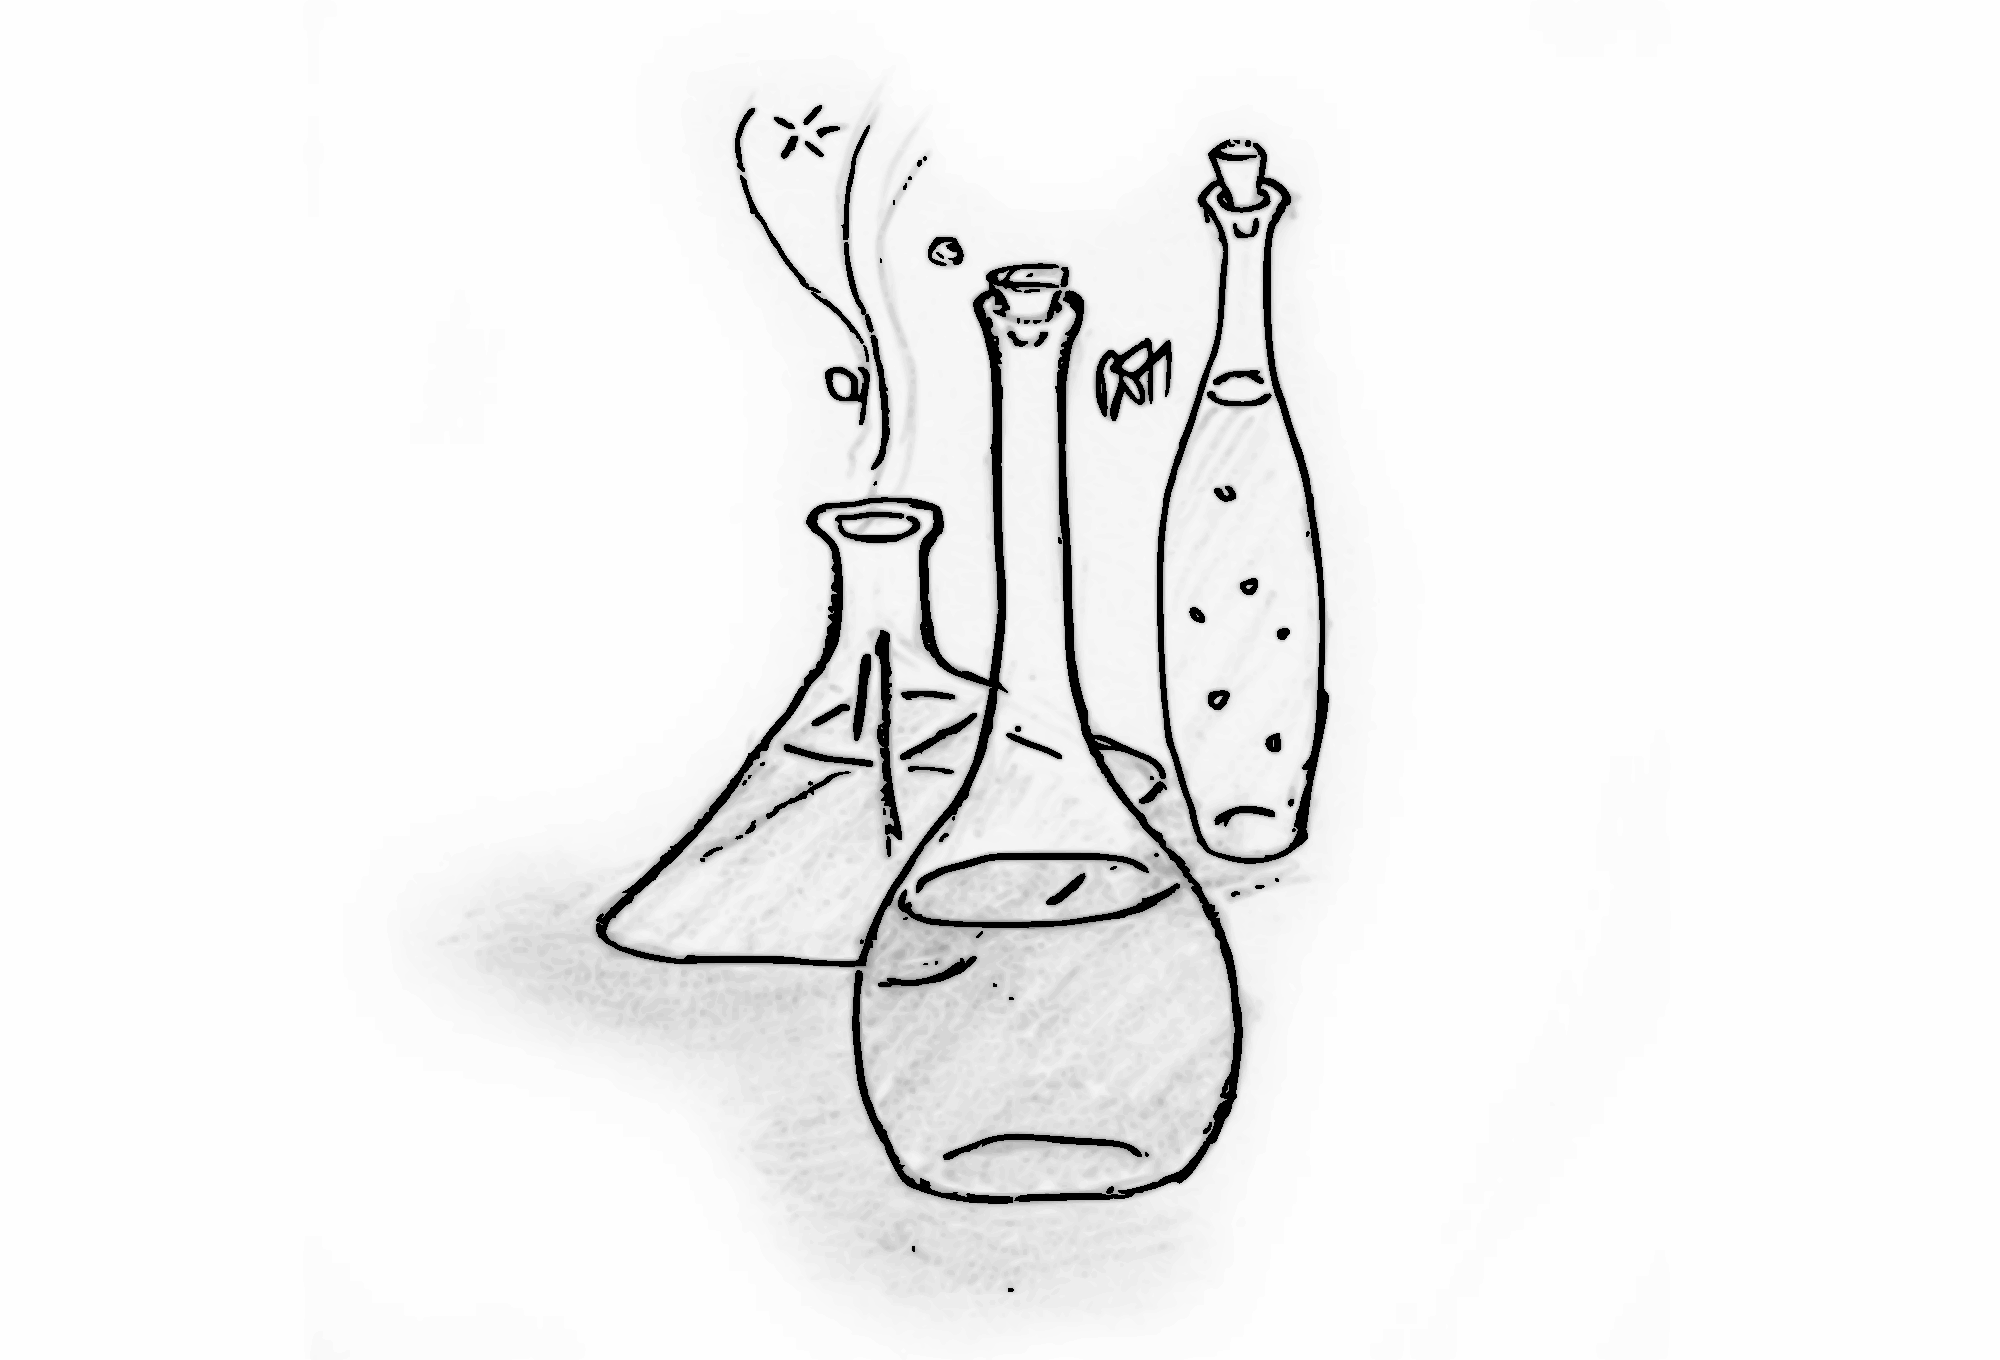
\includegraphics[width=\columnwidth]{vials.pdf}\label{vials}

\paragraph{Philter of Persuasiveness:} This potion grants the one who consumes it a +5 bonus to charisma---reaction modifier.  In addition, once per turn the consumer can make a suggestion to creatures within 30 yards (refer to the \textit{suggestion} spell).  Elves and half-elves retain their normal resistance to the charm effect, and each target is allowed a saving throw vs. spell to avoid the effect.

\paragraph{Philter of Stammering and Stuttering:} This accursed potion fools the one who consumes it into believing he has consumed either a \textit{philter of glibness} or \textit{philter of persuasiveness}.  However, whenever the consumer attempts to speak meaningfully (including parley with a creature, cast a spell, read a scroll, activate an item, etc.), all of the words are unintelligible and nonsensical.  The consumer suffers a $-5$ penalty to his charisma---reaction modifier while speaking like this.

\paragraph{Plant Control:} This potion allows the one who consumes it to immediately charm any normal plants, fungi, molds, and plant-like monsters within a 20-foot by 20-foot square up to 90 yards away (refer to the \textit{charm plant} spell).  Plants with intelligence of 5 or higher gain a save vs. spell to avoid the effect.  The potion's effect lasts 5d4 rounds.

\paragraph{Poisoned:} The GM is given free reigns when choosing the specific effects and origins of a poisoned potion.  He may select any type and strength of poison (refer to Poison) or create his own variety, however, the most common is an ingestion poison of strength type ``J".  As a general rule, poisoned potion gives off no distinguishing odor and can be of any color.  The typical poisoned potion takes effect even if merely sampled, however, they can be found in three strengths; weak (+4 to +1 bonus on the saving throw), average, and deadly ($-1$ to $-4$ penalty on the saving throw).  Some are so potent that a neutralize poison spell will not fully neutralize it and can only provide up to a +4 bonus to the save.  It seems there is at least a small amount of magical element in the making of these poisonous liquids.  Some may be potions that failed during the brewing or that spoiled after years of disuse, while others may come from secret formulas known only to master alchemists or assassins.  Poisoned potions are typically left as traps in a treasure hoard, but some, especially those of the contact (or gaseous) variety, may also be hurled as an indirect missile if the GM allows.

\paragraph{Polymorph Self:} This potion bestows upon the one who consumes it the ability to assume a different form as if he were affected by a \textit{polymorph self} spell (refer to the \textit{polymorph self} spell).  

\paragraph{Rainbow Hues:} This potion bestows upon the one who consumes it the ability to change the color of his body to any hue or combination of colors at will for the duration.  The consumer must simply think about the color change, and the change happens so quickly that up to 10 changes can be made in just a single round.  This potion always has the consistency of syrup, and loses its magical properties if not stored in a metal vial, or is otherwise exposed to light before being consumed.  Consuming a full vial produces an effect with duration of 7 hours, or a it can be divided into as many as seven doses with duration of one hour each.  Any similar and reasonable combination is allowed.

\paragraph{Speed:} This potion confers extra movement and attacks per round upon the one who consumes it as if he were affected by a haste spell for 5d4 rounds (refer to the \textit{haste} spell).  Consuming this potion permanently increases the consumer's age by one year if his venerable age is 150 years or less, 2 years if his venerable age is between 151 and 250 years, 3 years if his venerable age is between 251 and 350 years.

\paragraph{Super-Heroism:} This potion functions like an extra strength \textit{potion of heroism} which will only releases its true magic when consumed by one of the warrior class who is under 13\textsuperscript{th} level.  As with the \textit{potion of heroism}, the current level of the consumer determines the amount of bonus levels and temporary hit points gained.

\noindent
\begin{tabular}{|p{.25\columnwidth}|p{.25\columnwidth}|p{.35\columnwidth}|}
\hline
Warrior's Level	& Bonus Levels	& Hit Points \\
\hline\hline
\rowcolor[gray]{.9}0	& 6	& 5d10 \\
1st--3rd	& 5	& 4d10~+~1 \\
\rowcolor[gray]{.9}4th--6th	& 4	& 3d10~+~2 \\
7th--9th	& 3	& 2d10~+~3 \\
\rowcolor[gray]{.9}10th--12th	& 2	& 1d10~+~4 \\
\hline
\end{tabular}

\paragraph{Sweet Water:} This potion is harmless when sampled and tastes good, but it is not normally to be consumed.  Its true purpose is to turn any liquid with which it is mixed into clean, drinkable water.  A full vial is usually divided into 10 doses.  Each dose purifies up to 10,000 cubic feet of polluted, salty or alkaline contaminated water or up to 100 cubic feet of acid.  A single dose also has the power to automatically neutralize most poisons (in this case a poisoned creature may need to consume a dose) and when mixed with any other potion ruins the potion without the benefit of a save (even when both have been consumed).  The purified water radiates magic for 5d4 rounds and remains clean and uncontaminated for at least that long.

\paragraph{Treasure Finding:} This potion grants the one who consumes it the ability to detect the location of precious metals and/or gemstones.  The treasure cache must be within 240 yards and must contain metal equaling at least 10,000 coins (200 lbs. or more of precious metal) and/or 100 gems.  Any reasonable combination is allowed, but mundane and magical items not containing precious metals or gems are ignored.  The consumer knows the direction but not the exact location of the treasure.  Only magical wards and lead-lined walls block the potion's effects, which otherwise last 5d4 rounds.

\paragraph{Undead Control:} This potion grants the one who consumes it with the ability to control a specific type of undead for 5d4 rounds (refer to the \textit{charm} spell).  A maximum of 16 HD worth of undead can be controlled.  Ignore any bonuses to a creature's HD when calculating total HD.  The undead (other than mindless zombies and skeletons) are granted a saving throw vs. spell with a $-2$ penalty to avoid the effect.  Roll a 1d10 to determine the type of undead that the potion is effective against.  The GM may modify or add to this list as dictated by the needs of his world.

\noindent
\begin{tabular}{|p{.2\columnwidth}|p{.7\columnwidth}|}
\hline
1d10	& Type \\
\hline\hline
\rowcolor[gray]{.9}1	& Ghasts \\
2	& Ghosts \\
\rowcolor[gray]{.9}3	& Ghouls \\
4	& Shadows \\
\rowcolor[gray]{.9}5	& Skeletons \\
6	& Specters \\
\rowcolor[gray]{.9}7	& Wights \\
8	& Wraiths \\
\rowcolor[gray]{.9}9	& Vampires \\
10	& Zombies \\
\hline
\end{tabular}

\paragraph{Ventriloquism:} This potion allows the one who consumes it to throw his voice as if he were affected by a \textit{ventriloquism} spell.  The consumer can throw his voice up to six times within the effect's duration.

\paragraph{Vitality:} Consuming an entire vial of this potion removes the debilitating effects of exhaustion (mental or physical), hunger, and thirst from the one who consumes it.  Any current damage or effects from up to 7 days of recent deprivation are nullified immediately.  If the previous deprivation had lasted less than 7 days, the consumer won't need to sleep, eat, or drink for the remainder of the 7-day duration.  In addition, he becomes immune to poison and disease, and recovers from any type of damage at a rate of 1 hit point every 4 hours for the remainder of the duration.

\paragraph{Water Breathing:} This potion grants the one who consumes it the ability to breathe water as if he were affected by a \textit{water breathing} spell.  There's a 75\% chance that a full vial contains two doses, and a 25\% chance that it contains four.  Each dose lasts for one hour (6 turns).

\section{SCROLLS}

\index{Scrolls}Scrolls are scribed on heavy sheets of fine vellum, high-quality papyrus or paper.  The sheets are reinforced at the top and bottom with strips of leather slightly longer than the sheet is wide.  Scrolls greater than three feet long are usually fitted with reinforcing rods at each end rather than simple strips of leather.  To protect it from wrinkling or tearing, a scroll is rolled up from both ends to form a double cylinder.  This also helps the user unroll the scroll quickly.  

Scrolls are stored in ivory, jade, leather, metal, or wooden cases.  Commonly available scroll cases are plain and unadorned, but spell casters decorate and inscribe them with magic script and other unusual writing.  Often, these inscriptions hide magic traps, such as symbols, glyphs of warding, explosive runes, etc.  More practically, the writing may serve to identify the owner and/or the title of the scroll stored inside and must be read with the aid of a \textit{read magic} spell and possibly a \textit{comprehend languages} spell (refer to the \textit{wizard mark} spell).  In some cases, the writings must be read in order to open the scroll case.  The GM may treat this as a specialized \textit{wizard lock} spell on the scroll case, which is only released by a command word hidden within the wizard mark or other symbols.  

After a scroll has been opened, any character able to read it (see below) can scan it to learn its general contents.  Scanning the general contents of a scroll does not activate its magic, unless it is cursed or has a magic trap (as above) placed upon it.  The GM may determine that a scroll must be scanned immediately after being opened or the scroll will fade and the magic lost.  The GM may determine the percentage chance to fade by assigning a base 5\% and adding 5\% per year or part thereof after the first that the scroll case has laid unopened.  In this case, a scroll that has not been opened and scanned in over 20 years has a 100\% chance to fade if not scanned immediately.  Instead the GM may assume that most scrolls have not been left idle in their scroll cases much longer than 6 years on average.  In this case, the GM rolls 1d6 and multiplies the result by 5\% to determine a random chance to fade for each scroll found.  Scanning the scroll to determine the general nature of its content serves to renew the scroll's writings until it lies dormant once more.

Technically, scrolls can hold any manner of information, but the most important scrolls for the adventurer's purposes are found in four main varieties: map, spell (wizard or priest), protection and cursed scrolls.  

\noindent
\begin{minipage}{\columnwidth}

\captionof{table}{Scrolls (1d6)}\label{scrollsa}
\noindent
\begin{tabular}{|p{.12\columnwidth}|p{.55\columnwidth}|p{.18\columnwidth}|}
\multicolumn{3}{c}{Sub-Table A (1--2)} \\ 
\hline
1d20	& Type of Scroll	& XP \\
\hline\hline
\rowcolor[gray]{.9}1	& Map	& -- \\
2	& Protection---Acid	& 2,500 \\
\rowcolor[gray]{.9}3	& Protection---Cold	& 2,000 \\
4	& Protection---Dragon Breath	& 2,000 \\
\rowcolor[gray]{.9}5	& Protection---Electricity	& 1,500 \\
6--7	& Protection---Elementals	& 1,500 \\
\rowcolor[gray]{.9}8	& Protection---Fire	& 2,000 \\
9	& Protection---Gas	& 2,000 \\
\rowcolor[gray]{.9}10--11	& Protection---Lycanthropes	& 1,000 \\
12	& Protection---Magic	& 1,500 \\
\rowcolor[gray]{.9}13	& Protection---Petrification	& 2,000 \\
14	& Protection---Plants	& 1,000 \\
\rowcolor[gray]{.9}15	& Protection---Poison	& 1,000 \\
16	& Protection---Possession	& 2,000 \\
\rowcolor[gray]{.9}17	& Protection---Undead	& 1,500 \\
18	& Protection---Water	& 1,500 \\
\rowcolor[gray]{.9}19	& Cursed	& Accursed \\
20	& GM's Choice	& -- \\
\hline
\end{tabular}

\end{minipage}

\noindent
\begin{tabular}{|p{.15\columnwidth}|p{.35\columnwidth}|p{.35\columnwidth}|}
\multicolumn{3}{c}{Sub-Table B (3--6)} \\
\hline
1d20	& Number	& Spell Level* \\
\hline\hline
\rowcolor[gray]{.9}1--3	& 1 spell	& 1d4 \\
4--5	& 1 spell	& 1d6 \\
\rowcolor[gray]{.9}6	& 1 spell	& 1d8~+~1 (1d6~+~1) \\
7	& 2 spells	& 1d4 \\
\rowcolor[gray]{.9}8	& 2 spells	& 1d8~+~1 (1d6~+~1) \\
9	& 3 spells	& 1d4 \\
\rowcolor[gray]{.9}10	& 3 spells	& 1d8~+~1 (1d6~+~1) \\
11	& 4 spells	& 1d6 \\
\rowcolor[gray]{.9}12	& 4 spells	& 1d8 (1d6) \\
13	& 5 spells	& 1d6 \\
\rowcolor[gray]{.9}14	& 5 spells	& 1d8 (1d6) \\
15	& 6 spells	& 1d6 \\
\rowcolor[gray]{.9}16	& 6 spells	& 1d6~+~2 (1d4~+~2) \\
17	& 7 spells	& 1d8 \\
\rowcolor[gray]{.9}18	& 7 spells	& 1d8~+~1 (1d6~+~1) \\
19	& 7 spells	& 1d6~+~3 (1d4~+~3) \\
\rowcolor[gray]{.9}20	& GM's Choice	& -- \\
\hline
\end{tabular}
\noindent\begin{tabular}{p{.95\columnwidth}}
*Roll for each spell; the formulae in parenthesis are the level ranges for priest spells \\
\end{tabular}\vspace{.5em}

\paragraph{XP:} The experience value for scrolls containing spells is equal to the total spell levels contained on the scroll times 100.

\subsection{MAP SCROLLS}

\index{Scrolls!Map Scrolls}Map scrolls are not in and of themselves magical items and can be read by anyone.  Therefore, any character may scan a map to determine its general contents.  However, some maps (especially those containing important information and/or that might reveal the location of a large treasure hoard) may be written, at least partly, in ancient/obscure language(s) and/or magic script.  These maps require magical or other extraordinary methods, as determined by the GM, to reveal their full contents.  

Certainly small simple maps, of one page or less, are not uncommon, but a map scroll is not limited to a single page.  The scroll can be as many feet long as needed to include terrain maps, area maps, inset maps, illustrations; as well as notes, warnings, journal entries, etc.  A single ``map" to a distant land could easily consist of two or more scrolls. 

Sometimes, the GM may wish to include a map scroll as part of a treasure as a way to convey specific information relating to his world's storyline, but a map scroll can sometimes be found as a random item.  Finding a map scroll can mean a great adventuring opportunity for the characters.  The GM is therefore encouraged to include random treasure maps that do not overly interfere with his world's storyline or provide more information than he wishes the characters to know, yet provide just enough information to spur on a challenging side adventure for when the characters have the time.  A treasure map should imply a great hoard just waiting to be found by the right group of adventurers, but never reveal an amount and only provide the most vague references to the dangers involved.  There is no guarantee that the adventurers will be up to the challenge, or that the map is accurate or genuine.

The following tables can be used to randomly create a treasure map, whenever a map scroll is found for which the GM has no specific plans.

\noindent 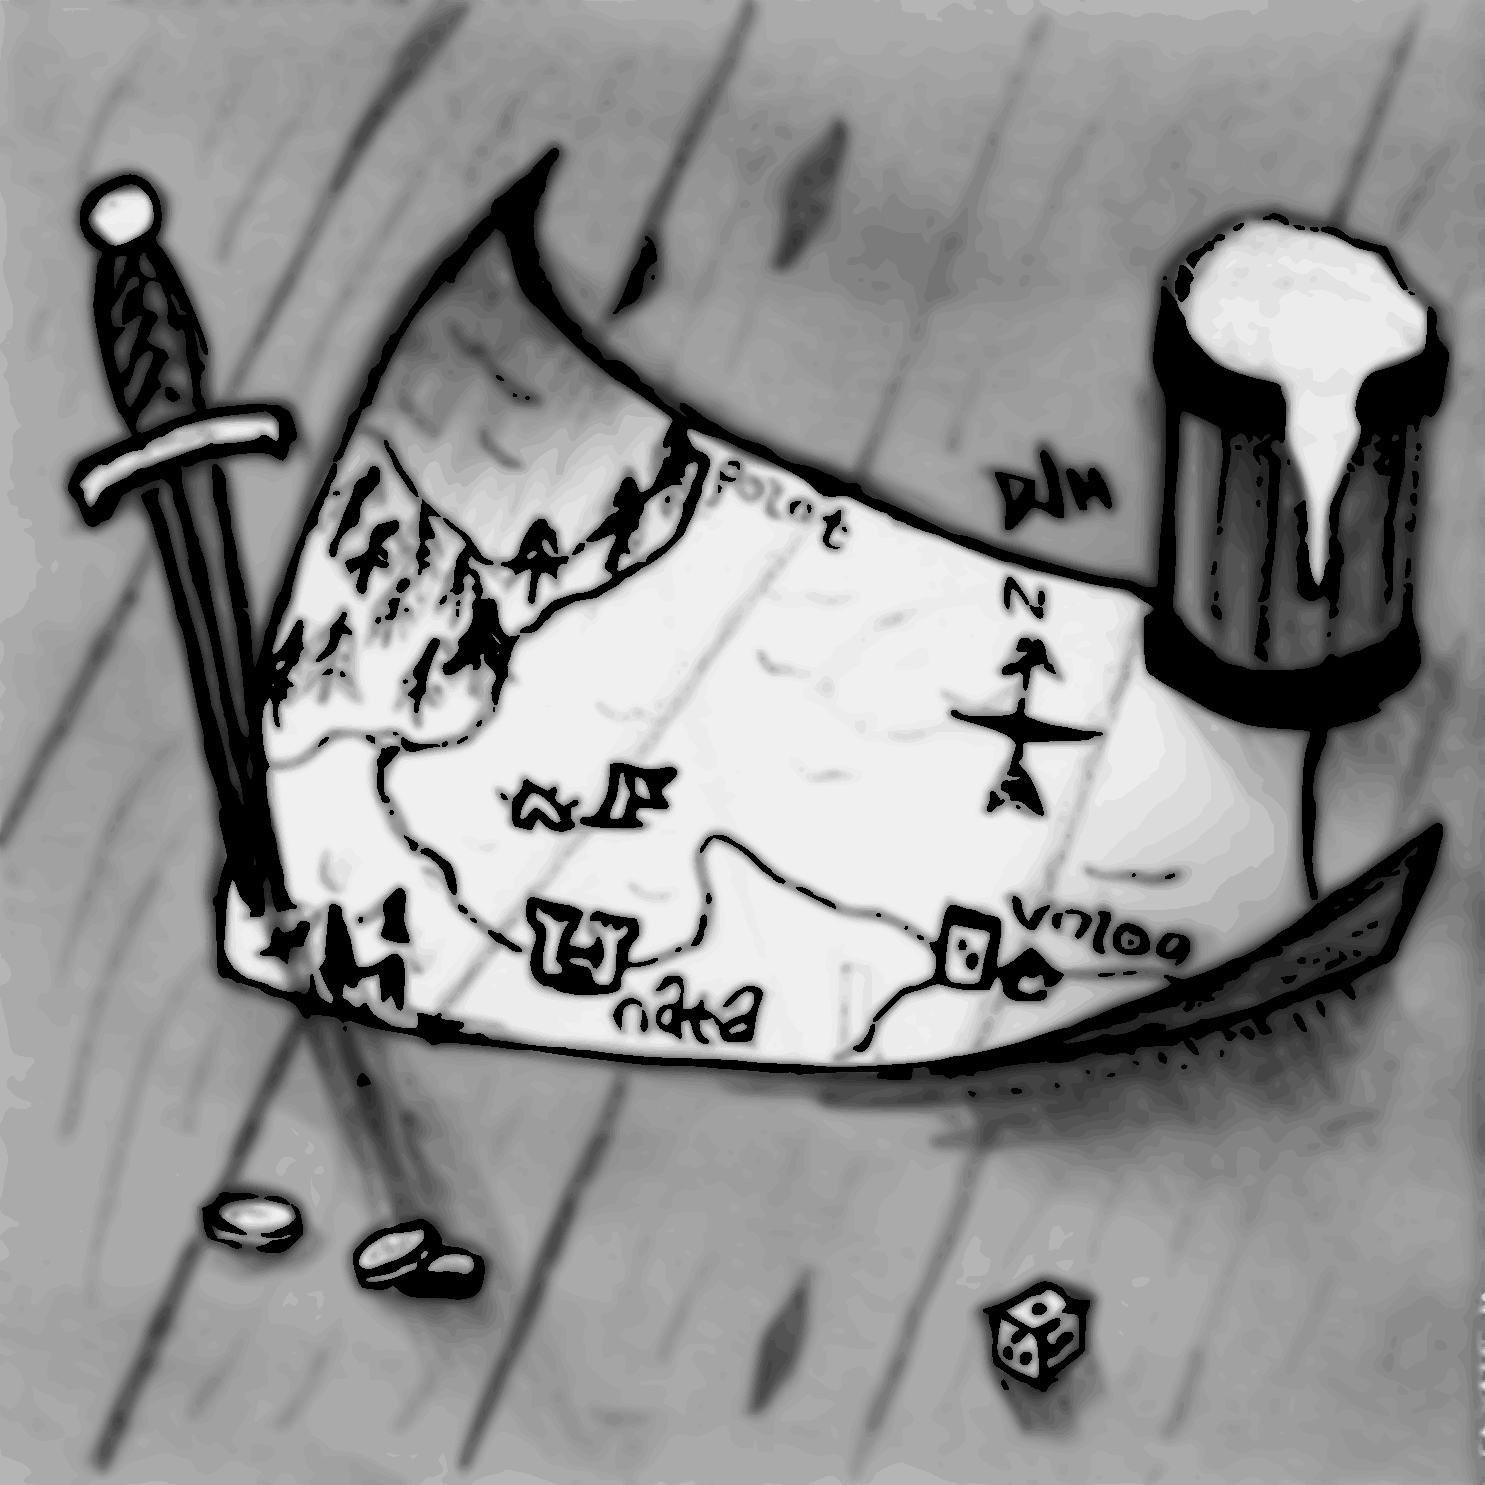
\includegraphics[width=\columnwidth]{treasuremap.pdf}\label{unionmap}

\paragraph{Type of Hoard:} The following table determines the type of treasure hoard.  Do NOT reveal the type of treasure hoard to the player characters.  The specific amount of treasure will be determined later.

\noindent
\begin{minipage}{\columnwidth}

\captionof{table}{Map Table}\label{typeofhoard}
\noindent
\begin{tabular}{|p{.12\columnwidth}|p{.78\columnwidth}|}
\hline
1d100	& Result\\
\hline\hline
\rowcolor[gray]{.9}01--05	& False map*.  One of the following has occurred: the treasure has already been looted (possibly ages ago), the map actually leads to a hazard or trap, it is a wild fantasy based solely on local legends, etc. \\
06--70	& Monetary hoard \\
\rowcolor[gray]{.9}71--90	& Magic hoard \\
91--00	& Combined hoard \\
\hline
\end{tabular}
\noindent\begin{tabular}{p{.95\columnwidth}}
*When a false map is determined, simply continue as if it was a valuable treasure map, but there is no need to determine the exact amount of the non-existent hoard. \\
\end{tabular}\vspace{.5em}

\end{minipage}

\paragraph{Distance:} The location revealed by the map can be only a few hundred feet away or up to several hundred miles away.  The GM must remember to take terrain features into account, and may choose the direction to best fit the shape of his world, or roll 1d8 to determine the direction randomly (1---North, 2---Northeast, 3---East, 4---Southeast, 5---South, 6---Southwest, 7---West, 8---Northwest).  The following table determines the distance to the treasure hoard and provides a treasure modifier.  The treasure modifier is added to the 1d20 roll when determining the amount of treasure in a hoard.  It is cumulative with the treasure modifier from the Map Location Table (next section).

\noindent
\begin{minipage}{\columnwidth}

\captionof{table}{Map Distance Table}\label{mapdistance}
\noindent
\begin{tabular}{|p{.15\columnwidth}|p{.5\columnwidth}|p{.2\columnwidth}|}
\hline
1d100	& Distance	& Treasure Modifier \\
\hline\hline
\rowcolor[gray]{.9}01--20	& 1d4~$-$~1 (0--3) miles	& $-4$ \\
21--60	& 1d4~+~6 (7--10) miles	& $-0$ \\
\rowcolor[gray]{.9}61--90	& 1d4~$\times$~10 (10--40) miles	& +1 \\
91--00	& 10d10~$\times$~4 (40--400) miles	& +2 \\
\hline
\end{tabular}

\end{minipage}

\paragraph{Location:} A treasure hoard may be hidden anywhere.  The following table lists some common, mundane places where treasure is often hidden and gives a treasure modifier (See Distance above).  Unless there is already a lair, body of water, crypt, hamlet, ruin or other appropriate feature conveniently located in approximately the correct place, this location should then also be noted on the main map of the GM's world.

\noindent
\begin{minipage}{\columnwidth}

\captionof{table}{Map Location Table}\label{maplocation}
\noindent
\begin{tabular}{|p{.15\columnwidth}|p{.5\columnwidth}|p{.2\columnwidth}|}
\hline
1d100	& Location	& Treasure Modifier \\
\hline\hline
\rowcolor[gray]{.9}01--10	& Buried and unguarded	& $-4$ \\
11--20	& Under water	& $-2$ \\
\rowcolor[gray]{.9}21--70	& Creature's lair	& $-$0 \\
71--80	& Burial crypt	& +0 \\
\rowcolor[gray]{.9}81--90	& Ruins	& +1 \\
91--00	& Community	& +2 \\
\hline
\end{tabular}

\end{minipage}

\paragraph{Treasure Guardians:} Unless buried, treasure hoards are nearly always well protected by appropriate creatures (whether magical, mundane or undead).  The GM must choose appropriate guardian creatures based upon the hoard's value (next section), and chances for encountering wandering monsters occur normally while following the map.  Some or all of these hazards may be indicated on the treasure map, but if they are, they are almost always given in a vague or cryptic manner.

The GM now has more than enough information to provide a treasure map to the characters.  

\paragraph{Value of the Treasure Hoard:} Roll 1d20, add or subtract the combined treasure modifier from the Map Distance and Location Tables (if any), and consult the appropriate hoard table (Monetary, Magic or Combined from the Map Table) to determine how much treasure and in what form.  It is suggested that these hoards consist mainly of bulk coins, heavy objects that are difficult to transport, or even well known items with questionable origins which prove difficult to sell.

\noindent
\begin{minipage}{\columnwidth}

\captionof{table}{Monetary Hoard Table}\label{hoardtype}
\noindent
\begin{tabular}{|p{.15\columnwidth}|p{.6\columnwidth}|p{.1\columnwidth}|}
\hline
1d20	& Result	& Code \\
\hline\hline
\rowcolor[gray]{.9}1--2	& 20,000--80,000 (2d4 $\times$ 10,000) copper pieces \& 
20,000--50,000 ((1d4~+~1) $\times$ 10,000) silver pieces	& A \\
3--5	& 5,000--30,000 (5d6 $\times$ 1000) electrum pieces	& B \\
\rowcolor[gray]{.9}6--10	& 3,000--18,000 (3d6 $\times$ 1000) gold pieces	& C \\
11--12	& 500--2,000 (5d4 $\times$ 100) platinum pieces	& D \\
\rowcolor[gray]{.9}13--15	& 10--100 (d10 $\times$ 10) gemstones	& E \\
16--17 	& 5--50 (5d10) objects of art	& F \\
\rowcolor[gray]{.9}18	& Roll twice, discard rolls above 17	& G \\
19	& Roll three times, discard rolls above 17	& H \\
\rowcolor[gray]{.9}20	& Roll four times, discard rolls above 17	& I \\
\hline
\end{tabular}

\end{minipage}

\noindent
\begin{minipage}{\columnwidth}

\captionof{table}{Magic Hoard Table}\label{magichoardtype}
\noindent
\begin{tabular}{|p{.15\columnwidth}|p{.6\columnwidth}|p{.1\columnwidth}|}
\hline
1d20	& Result	& Code \\
\hline\hline
\rowcolor[gray]{.9}1--5	& Any magic item, plus 4 potions	& A \\
6--8	& Any 2 magic items	& B \\
\rowcolor[gray]{.9}9--12	& 1 sword, 1 armor or shield, \& 1 miscellaneous weapon	& C \\
13--14	& Any 3 items, except sword or potions	& D \\
\rowcolor[gray]{.9}15--18	& Any 6 potions and any 6 scrolls (possibly including a map)	& E \\
19	& Any 4 items, 1 of which is a ring \& 1 of which is a rod	& F \\
\rowcolor[gray]{.9}20	& Any 5 items, 1 of which is a rod \& 1 is miscellaneous item	& G \\
\hline
\end{tabular}

\end{minipage}

\noindent
\begin{minipage}{\columnwidth}

\captionof{table}{Combined Hoard Table}\label{combinedhoardtype}
\noindent
\begin{tabular}{|p{.15\columnwidth}|p{.75\columnwidth}|}
\hline
1d20	& Result Code(s) \\
\hline\hline
\rowcolor[gray]{.9}1--4	& Monetary hoard A \& magic hoard A \\
5--8	& Monetary hoard C \& magic hoard A \\
\rowcolor[gray]{.9}9--11	& Monetary hoard B, C \& magic hoard A, E \\
12--13	& Monetary hoard A, B, C \& magic hoard C, D \\
\rowcolor[gray]{.9}14--15	& Monetary hoard C, D \& magic hoard B, E \\
16	& Monetary hoard B, C, D, F \& magic hoard A, C \\
\rowcolor[gray]{.9}17	& Monetary hoard A, B, C, D, E, F \& a map to magic hoard A \\
18	& Monetary hoard A, B, C, D, E, F \& a map to magic hoard F \\
\rowcolor[gray]{.9}19	& Magic hoard G \& a map to monetary hoard A, B \\
20	& Magic hoard G \& a map to monetary hoard D, E~+~magic hoard E \\
\hline
\end{tabular}

\end{minipage}

\paragraph{Treasure Containers:} Treasure hoards may be left loose but more often are stored in one or more containers of various sizes and shapes.  This table can help the GM determine how the treasure hoard is stored.  He may roll or select as many containers as necessary to account for the entire hoard satisfactorily.

\noindent
\begin{minipage}{\columnwidth}

\captionof{table}{Treasure Container Table}\label{treasurecontainer}
\noindent
\begin{tabular}{|p{.2\columnwidth}|p{.7\columnwidth}|}
\hline
1d20	& Container \\
\hline\hline
\rowcolor[gray]{.9}1--2	& Bag \\
3--4	& Sack \\
\rowcolor[gray]{.9}5--6	& Small Coffer \\
7--8	& Chest \\
\rowcolor[gray]{.9}9--10	& Huge Chest \\
11--12	& Pottery Jar \\
\rowcolor[gray]{.9}13--14	& Metal Urn \\
15--16	& Stone Container \\
\rowcolor[gray]{.9}17--18	& Iron Trunk \\
19--20	& Loose \\
\hline
\end{tabular}

\end{minipage}

\noindent
\includegraphics[width=3.6in, height=2.75in]{testblock.pdf}

\paragraph{Traps on the container:} A treasure hoard usually carries a mundane or magical trap.  This is entirely the purview of the GM as to what kind of trap and how the trap works.  The GM determines one or more traps per container, as appropriate.  The following table provides some ideas on how to trap common containers.

\noindent
\begin{minipage}{\columnwidth}

\captionof{table}{Treasure Traps}\label{treasuretraps}
\noindent
\begin{tabular}{|p{.15\columnwidth}|p{.75\columnwidth}|}
\hline
1d20	& Trap \\
\hline\hline
\rowcolor[gray]{.9}1--4	& Contact poison on container and/or treasure (GM determines exact type (refer to Poisons)) \\
5--7	& Poisoned needles in lock or handles (GM determines exact type (refer to Poisons)) \\
\rowcolor[gray]{.9}8--10	& Spring darts fire from front of container, top of container or from inside bottom of container. \\
11--12	& Blade scything across inside \\
\rowcolor[gray]{.9}13	& Venomous insects or reptiles living inside container \\
14	& Poison gas released by opening container \\
\rowcolor[gray]{.9}15--16	& Trapdoor opens 1d6 feet in front of container \\
17	& Stone block drops in front of the container \\
\rowcolor[gray]{.9}18	& Spears fire from walls when container opened \\
19	& Explosive runes \\
\rowcolor[gray]{.9}20	& Symbol \\
\hline
\end{tabular}

\end{minipage}

\paragraph{Hiding the hoard:} Whether trapped or not, the whole hoard may be hidden by mundane or magical means.  The GM determines an appropriate method to hide the hoard, if any.  The following table provides some ideas on how to hide a treasure hoard.

\noindent
\begin{minipage}{\columnwidth}

\captionof{table}{Treasure Hiding}\label{treasurehiding}
\noindent
\begin{tabular}{|p{.15\columnwidth}|p{.75\columnwidth}|}
\hline
1d20	& Result \\
\hline\hline
\rowcolor[gray]{.9}1--3	& Invisibility \\
4--5	& Illusion (to change or hide its appearance) \\
\rowcolor[gray]{.9}6	& Secret space under container \\
7--8	& Secret compartment inside container \\
\rowcolor[gray]{.9}9	& Inside an ordinary item in plain view \\
10	& Disguised to appear as something else \\
\rowcolor[gray]{.9}11	& Under a heap of trash/dung \\
12--13	& Under a loose stone in the floor \\
\rowcolor[gray]{.9}14--15	& Behind a loose stone in the wall \\
16--20	& In a secret room nearby \\
\hline
\end{tabular}

\end{minipage}

\subsection{SPELL SCROLLS}

\index{Scrolls!Spell Scrolls}A spell scroll is a spell (or collection of spells) that has been stored in written form.  Due to the unpredictable nature of magical writing, a spell scroll can contain no more than 7 spells.  The writing vanishes from the scroll when the spell is activated, so that a spell can be used only once from a scroll.  Reading a spell scroll is basically like casting the spell, including casting time.  The caster must maintain concentration while reading the scroll aloud (as if he were casting the spell), or the spell fails and disappears from the scroll.  A scroll will allow a caster to cast a spell, which he is not normally able to cast, whether due to level, intelligence, wisdom, sphere or school restrictions, etc. 

Spell scrolls contain wizard spells 70\% of the time and priest spells 30\% of the time.  Only a wizard can scan and read wizard scrolls and only a priest can scan and read priest scrolls, with the exception of high level thieves and bards who can scan and read any spell scroll.  Paladins and rangers can never scan or read spell scrolls.

\paragraph{Caster Levels:} The caster level of a spell found on a scroll is equivalent to the caster's level when the scroll was scribed, so can never be below 7\textsuperscript{th} level.  Generally speaking, the caster level of a random scroll is assumed to be the minimum level required to cast the spell plus one, but never below 7\textsuperscript{th}.  It can then be assumed that a 1\textsuperscript{st} through 3\textsuperscript{rd} level spell is scribed at 7\textsuperscript{th} level, while the 4\textsuperscript{th} level spell is scribed at 8\textsuperscript{th} level, a 5\textsuperscript{th} level spell at 10\textsuperscript{th}, a 6\textsuperscript{th} level spell at 12\textsuperscript{th} (Priest) or 13\textsuperscript{th} (Wizard), 7\textsuperscript{th} at 15\textsuperscript{th}, 8\textsuperscript{th} at 17\textsuperscript{th} and 9\textsuperscript{th} level spell at 19\textsuperscript{th} caster level.  This can be used as a basic guideline, but the GM is free to create spell scrolls scribed by spell casters of higher level (but not lower).  For example, a scroll containing both a 1\textsuperscript{st} and a 5\textsuperscript{th} level spell may be scribed at 7\textsuperscript{th} and 10\textsuperscript{th} caster levels respectively, or both spells may be scribed at 10\textsuperscript{th} level or even higher.  This choice however, directly affects the chance for magical spell failure (see below).

\paragraph{Magical Spell Failure:} When a high level rogue attempts to read a spell scroll, refer to their class listing for details.  Otherwise, when a spell caster attempts to read a spell scroll scribed at a caster level higher than his caster level, there's a chance for the spell activation to fail.  The percentage chance for failure to occur is equal to 5\% times the difference between the scroll's caster level and the caster level of the spell caster.  For example, a 3\textsuperscript{rd} level mage finds a spell scroll containing a 1\textsuperscript{st} level spell.  Assuming standard casting level for the scroll is 7\textsuperscript{th}, the mage has a 20\% chance of spell failure ((7~$-$~3)~$\times$~5\%).  If the 3\textsuperscript{rd} level mage attempts to read a spell scroll scribed at 13\textsuperscript{th} level (for any spell of up to and including 6\textsuperscript{th} level), his failure chance would be 50\% ((13~$-$~3)~$\times$~5\%).  A failed activation erases the spell from the scroll, and the GM must consult Table B.22: Spell Failure to determine if the attempt is harmful (attack spells target the caster and his allies, beneficial spells target enemies, etc,).  In the first example above, there is a 15\% chance of a harmful effect to occur (7~$-$~3) = a caster level difference of 4, while in the second example, there is a 35\% chance (13~$-$~3) = 10.

\noindent
\begin{minipage}{\columnwidth}

\captionof{table}{Spell Failure}\label{spellfailure}
\noindent
\begin{tabular}{|p{.45\columnwidth}|p{.45\columnwidth}|}
\hline
Caster Level Difference	& Harmful Effect \\
\hline\hline
\rowcolor[gray]{.9}1--3	& 5\% \\
4--6	& 15\% \\
\rowcolor[gray]{.9}7--9	& 25\% \\
10--12	& 35\% \\
\rowcolor[gray]{.9}13--15	& 50\% \\
16+	& 70\% \\
\hline
\end{tabular}

\end{minipage}

\paragraph{Using Spell Scrolls:} If the spell caster or rogue is successful in activating the spell from the scroll, all effects of the spell proceed normally at the scroll's caster level.

\paragraph{Permanent Spell Scrolls:} These potent magical items are extremely rare and are only placed by the GM under special circumstances.  Permanent scrolls can be read more than once, as the writing returns after a set period of time, such as once a day, week, month or even once a year.  Caster level and all other details are left to the GM.

\subsection{PROTECTION SCROLLS}

\index{Scrolls!Protection Scrolls}Protection scrolls can be scanned and read by any character class.  They can only be read once, and their writing disappears as the scroll is being read aloud.  Protection scrolls have a reading time that is analogous to a spell's casting time.  If the one who reads the scroll is disturbed during this time, the protection is lost and the writing disappears.  The size of the scroll is a function of its reading time.  For a reading time up to 3, the scroll is one foot long, between 4 and 6, two feet long, between 7 and 9, three feet long, and for a reading time of one round the scroll is four feet long. 

Some protection scrolls protect just the reader, while others create an effective area of protection.  An effective area is nearly always centered on the reader and moves with him.  Effects from reading multiple protection scrolls are cumulative for as long as the durations and effective areas overlap.  Protection scrolls can never be used offensively, so if the reader willingly forces an affected creature into a situation from which there is no retreat or escape (wall, trap, other dangerous area, etc.), the protection effect immediately ends.

\subsection{PROTECTION SCROLL DESCRIPTIONS}

\noindent \begin{minipage}{\columnwidth}

\noindent \textbf{Protection from Acid}

\noindent Reading Time: 6

\noindent Effective Area: Self

\noindent Duration: 1d4~+~8 turns

\end{minipage}

The reader is protected from all forms of acid damage up to a maximum of 20d8 points of damage or for the duration whichever comes first.

\vspace{1em}
\noindent \begin{minipage}{\columnwidth}

\noindent \textbf{Protection from Cold}

\noindent Reading Time: 3

\noindent Effective Area: 30-foot diameter sphere

\noindent Duration: 1d4~+~4 turns

\end{minipage}

This scroll generates a field of protection from cold for the duration.  All within the effective area are protected against any and all mundane cold.  The effect grants a +6 bonus to saves vs. magical cold and reduces damage to only one-quarter if the save fails and one-eighth if the save is successful.

\vspace{1em}
\noindent \begin{minipage}{\columnwidth}

\noindent \textbf{Protection from Dragon Breath}

\noindent Reading Time: 7

\noindent Effective Area: Self

\noindent Duration: 2d4~+~4 rounds

\end{minipage}

The reader is protected from the breath weapon of any dragon for the duration. 

\vspace{1em}
\noindent \begin{minipage}{\columnwidth}

\noindent \textbf{Protection from Electricity}

\noindent Reading Time: 5

\noindent Effective Area: 20-foot diameter sphere

\noindent Duration: 3d4 rounds

\end{minipage}

This scroll generates a field of protection from electricity that renders everyone within the effective area immune to any damage or other effects of electricity for the duration.

\vspace{1em}
\noindent \begin{minipage}{\columnwidth}

\noindent \textbf{Protection from Elementals}

\noindent Reading Time: 6

\noindent Effective Area: 10-foot diameter circle

\noindent Duration: 5d8 rounds

\end{minipage}

This scroll generates a field of protection that prevents physical contact between those within the effective area and specific elemental creatures.  Those elemental creatures mentioned in the scroll are pushed harmlessly to the edge of the effective area.  The specified elemental creatures cannot enter the effective area or attack those inside the effective area with melee attacks (and vice versa) for the duration or until the maximum HD (refer to the table below) is exceeded.  Those inside the invisible barrier can act and attack with thrown or missile weapons normally, but they must leave the protective barrier to perform melee attacks.  

There are several known varieties of this scroll.  To determine the variety randomly, roll 1d100.  The GM may expand this table, if desired, by including the quasi and para-elemental planes, as well as additional combinations.

\noindent
\begin{tabular}{|p{.15\columnwidth}|p{.75\columnwidth}|}
\hline
1d100	& Elemental Type \\
\hline\hline
\rowcolor[gray]{.9}01--15	& Air elementals, aerial servants, djinn, invisible stalkers, wind walkers, etc. (up to 24 HD) \\
16--30	& Earth elementals, xorn, etc. (up to 24 HD) \\
\rowcolor[gray]{.9}31--45	& Fire elementals, efreeti, salamanders, etc. (up to 24 HD) \\
46--60	& Water elementals, tritons, water weirds, etc. (up to 24 HD) \\
\rowcolor[gray]{.9}61--00	& Elementals and any other creatures from the elemental planes (up to 16 HD) \\
\hline
\end{tabular}

\vspace{1em}
\noindent \begin{minipage}{\columnwidth}

\noindent \textbf{Protection from Fire}

\noindent Reading Time: 8

\noindent Effective Area: 30-foot diameter sphere

\noindent Duration: 1d4~+~4 turns

\end{minipage}

This scroll generates a field of protection centered on the reader that renders all creatures within the effective area immune to any and all fire damage for the duration.

\columnbreak
 
\vspace{1em}
\noindent \begin{minipage}{\columnwidth}

\noindent \textbf{Protection from Gas}

\noindent Reading Time: 3

\noindent Effective Area: 10-foot diameter circle

\noindent Duration: 1d4~+~4 rounds

\end{minipage}

This scroll generates a field of protection that renders everyone within the effective area immune to all gases and/or toxic vapors, mundane or magical, for the duration.

\vspace{1em}
\noindent \begin{minipage}{\columnwidth}

\noindent \textbf{Protection from Lycanthropes}

\noindent Reading Time: 4

\noindent Effective Area: 10-foot diameter circle

\noindent Duration: 5d6 rounds

\end{minipage}

This scroll generates a field of protection that prevents physical contact between those within the effective area and specific lycanthropes.  Those lycanthropes mentioned in the scroll are pushed harmlessly to the edge of the effective area.  The specified lycanthropes cannot enter the effective area or attack those inside the effective area with melee attacks (and vice versa) for the duration or until 49 HD is exceeded.  If the creature has a hit point adjustment of +3 or more, round up to the next HD when calculating the total.  Those inside the invisible barrier can act and attack with thrown or missile weapons normally, but they must leave the protective barrier to perform melee attacks.  

There are several known varieties of this scroll.  To determine the variety randomly, roll 1d100.  The GM may expand this table, if desired, by including lycanthropes or other shape-changers, as well as additional combinations.

\noindent
\begin{tabular}{|p{.15\columnwidth}|p{.75\columnwidth}|}
\hline
1d100	& Type \\
\hline\hline
\rowcolor[gray]{.9}01--05	& Werebears \\
06--10	& Wereboars \\
\rowcolor[gray]{.9}11--20	& Wererats \\
21--25	& Weretigers \\
\rowcolor[gray]{.9}26--40	& Werewolves \\
41--98	& All lycanthropes \\
\rowcolor[gray]{.9}99--00	& All shape-changers* \\
\hline
\end{tabular}
\noindent\begin{tabular}{p{.95\columnwidth}}
*The powerful protection from ``all shape-changers" protects against any creatures (except demigods and deities) that can change their shape to or from a human form (such as dopplegangers, some dragons, druids, jackalweres, mages using the \textit{shape change} spell, etc., but not including those using polymorph effects). \\
\end{tabular}\vspace{.5em}

\vspace{1em}
\noindent \begin{minipage}{\columnwidth}

\noindent \textbf{Protection from Magic}

\noindent Reading Time: 8

\noindent Effective Area: 5-foot radius globe

\noindent Duration: 5d6 rounds

\end{minipage}

This scroll generates a field of protection blocking all magical effects from entering, exiting or operating within the effective area for the duration.  Creatures, including those summoned or otherwise magical in nature, and physical objects, such as magical weapons, ammunition, armor, and other magical items, are unaffected.  However, magical effects (other than enchantment modifiers) from these items cannot pass through or operate within the barrier. A \textit{dispel magic} is ineffective against the effects of this scroll.

\vspace{1em}
\noindent \begin{minipage}{\columnwidth}

\noindent \textbf{Protection from Petrification}

\noindent Reading Time: 5

\noindent Effective Area: 10-foot radius circle

\noindent Duration: 5d4 rounds

\end{minipage}

This scroll generates a field that protects all creatures within the effective area from any attack causing petrification, magical or otherwise, for the duration.

\vspace{1em}
\noindent \begin{minipage}{\columnwidth}

\noindent \textbf{Protection from Plants}

\noindent Reading Time: 1

\noindent Effective Area: 10-foot diameter sphere

\noindent Duration: 1d4~+~4 turns

\end{minipage}

This scroll generates a field of protection that prevents physical contact between those within the effective area and all forms of living vegetable matter including fungi, slimes, and molds.  Mobile or unsecured plant-based creatures are pushed harmlessly to the edge of the effective area.  Inanimate plants (grass, trees, shrubs, etc.) can also be uprooted and pushed away, provided that the reader has the physical mass or strength score to do so ordinarily.  If the reader of the scroll does not have the physical mass or strength to move a plant (for example a large shrub or tree), the barrier will either go around the plant or collapse.  No plant-based creature can enter the effective area or attack those inside the effective area with melee attacks (and vice versa) for the duration.  Those inside the invisible barrier can act and attack with thrown or missile weapons normally, but they must leave the protective barrier to perform melee attacks.  

\vspace{1em}
\noindent \begin{minipage}{\columnwidth}

\noindent \textbf{Protection from Poison}

\noindent Reading Time: 3

\noindent Effective Area: Self

\noindent Duration: 1d10~+~2 rounds

\end{minipage}

Reading this scroll immediately neutralizes all poisons currently afflicting the reader and renders him immune to any and all poisons (contact, gas, etc.) for the duration.

\vspace{1em}
\noindent \begin{minipage}{\columnwidth}

\noindent \textbf{Protection from Possession}

\noindent Reading Time: 1 round

\noindent Effective Area: 10-foot radius circle

\noindent Duration: 10d6 rounds

\end{minipage}

This scroll generates a field of protection against all forms of possession, magic or otherwise, such as \textit{magic jar}, effects that directly dominate another creature's mind or other types of possession attacks.  The invisible barrier protects all creatures (including dead creatures) within the effective area for the duration.

Some 10\% of these scrolls create an effect with a duration of 10d6 turns but which does not move with the reader.

\vspace{1em}
\noindent \begin{minipage}{\columnwidth}

\noindent \textbf{Protection from Undead}

\noindent Reading Time: 4

\noindent Effective Area: 5-foot radius circle

\noindent Duration: 10d8 rounds

\end{minipage}

This scroll generates a field of protection that prevents physical contact between those within the effective area and all forms of the undead.  The undead are pushed harmlessly to the edge of the effective area.  They cannot enter the effective area or attack those inside the effective area with melee attacks (and vice versa) for the duration or until 35 HD is exceeded.  If the creature has a hit point adjustment of +3 or more, round up to the next HD when calculating the total.  Those inside the invisible barrier can act and attack with thrown or missile weapons normally, but they must leave the protective barrier to perform melee attacks.  

The GM may determine that there are many varieties of this scroll, each affecting a specific type or combination of types of undead rather than all types of undead.  The GM may refer to the \textit{potion of undead control} to determine a specific type of undead or to create various combinations.

\vspace{1em}
\noindent \begin{minipage}{\columnwidth}

\noindent \textbf{Protection from Water}

\noindent Reading Time: 6

\noindent Effective Area: 10-foot diameter sphere

\noindent Duration: 1d4~+~4 turns

\end{minipage}

This scroll generates a field of protection that prevents those inside the effective area from coming into contact with any solid, liquid, or gaseous form of water.  Any and all forms of water pass harmlessly over, under or around the sphere.  Those protected cannot be burned by steam, sink into a body of water, slip on an icy floor, etc.  Immobile solid pieces and sheets of ice are ignored, but do not make contact with those protected. 

\subsection{CURSED SCROLLS}

\index{Scrolls!Cursed Scrolls}A cursed scroll can appear as a scroll of another type, until it has been both opened and scanned (choose type and roll 1d10 for length in feet).  While a cursed scroll always radiates an aura of magic when \textit{detect magic} is cast, it will almost never radiate evil or other special aura.  The GM is free to determine the nature and origin of any cursed scrolls in his game.  Cursed scrolls may be created as an intentional trap or accidentally created during a failed attempt to scribe the other type of scroll (refer to Scribing Scrolls).

Regardless of what they appear to be, cursed scrolls activate the moment they are scanned.  Their effects are entirely within the GM's realm and can have any effect he determines.  Curses usually range from minor annoyances to slightly debilitating effects, and truly deadly curses are generally rare.  Most curses are permanent until negated by a \textit{remove curse} spell.  However, the GM may determine that more powerful and/or permanent effects, such as petrification, may require other methods of reversal (in this case, transmute stone to flesh).  

Rating curses based on their relative strengths is highly subjective.  For example, a mage, forced to take a vow of poverty, would give away his extremely valuable spell book and would not consider that to be a weak curse.  The GM has the final decision regarding the effects of curses.  Some sample curses include:

\noindent \underline{Weak Curses}

\begin{itemize}
\item Reader attacked by a randomly summoned 1\textsuperscript{st}--3\textsuperscript{rd} level monster
\item Reader affected by a random wizard or priest spell of up to 3\textsuperscript{rd} level with a caster level of at least 7
\item Reader randomly teleports 2d6 miles away
\item Reader suffers 2d6 points of damage, no save
\item Reader suffers from bad luck ($-1$ attack rolls, saving throws, ability checks, etc.)
\item Reader's strength is halved
\item Reader swears a vow of poverty and donates all his possessions to charity
\end{itemize}

\noindent \underline{Moderate Curses}

\begin{itemize}
\item Reader attacked by a randomly summoned 4\textsuperscript{th}--6\textsuperscript{th} level monster
\item Reader affected by a random wizard spell of between 4\textsuperscript{th} and 6\textsuperscript{th} level (or priest spell of 4\textsuperscript{th} or 5\textsuperscript{th} level) with a caster level of at least 13 (or 10 for a priest spell)
\item Reader randomly teleports 2d6~$\times$~10 miles away
\item Reader suffers 4d6 points of damage, no save
\item Reader suffers from terrible luck ($-2$ attack rolls, saving throws, ability checks, etc.)
\item Reader's facial hair grows one inch per minute
\item Reader shrinks to half his size
\item Reader's appetite becomes insatiable
\item Reader is stricken with amnesia
\item Reader polymorphs into a harmless animal
\end{itemize}

\noindent \underline{Strong Curses}

\begin{itemize}
\item Reader attacked by a randomly summoned 7\textsuperscript{th}--10\textsuperscript{th} level monster
\item Reader affected by a random wizard spell between 7\textsuperscript{th} and 9\textsuperscript{th} level (or priest spell between 6\textsuperscript{th} and 7\textsuperscript{th} level) with a caster level of at least 19 (or 15 for a priest spell)
\item Reader randomly teleports 2d6~$\times$~100 miles away
\item Reader suffers 8d6 points of damage, no save
\item Reader suffers from horrendous luck ($-4$ attack rolls, saving throws, ability checks, etc.)
\item Reader falls into a comatose state and cannot be awakened by normal means
\item Reader can only speak in rhymes and cannot cast spells with verbal components
\item Reader changes to the diametrically opposed alignment
\item Reader must save vs. petrification or be turned to stone
\item Reader polymorphs into a liquid and drains away
\item Reader polymorphs into a creature equal to his character level and attacks the nearest creature
\end{itemize}

\noindent
\includegraphics[width=3.6in, height=2.75in]{testblock.pdf}

\section{MAGICAL RINGS}

\index{Rings}Magical rings bestow specific powers upon those who wear them.  A ring's power may be activated by speaking a command word or simply by concentrating on the desired power, or its power may be continuously active.  However, some magical rings have exceptional activation methods, detailed in their descriptions.  Sometimes a power activates immediately, while other times, the powers require time to activate.

No two magical rings look alike.  The vast majority of magical rings are forged from precious metals such as gold, silver, and platinum, but magical rings can exist crafted from glass, ivory, bone, etc.  

Most magical rings can benefit any creature; so long as the creature can wear the ring properly and is able to perform whatever action is needed to activate its powers.  Magical rings are only effective for humans, demi-humans and humanoids when worn on the fingers of the hands, or in the case of creatures that are not human-shaped, when worn on their primary manipulating digits.  A magical ring automatically resizes to fit the wearer's digit.  A creature can wear only two magical rings at the same time, and only one can be worn on each hand or other appendage.  If these restrictions are exceeded, all magical rings worn by the creature are rendered ineffective.  

Magical rings are indistinguishable from their mundane counterparts without means of divination magic and experimentation, appearing as appropriately expensive and well-crafted jewelry.  Most magical rings radiate an aura of magic commensurate with their powers when \textit{detect magic} is cast, but no known ring radiates an aura of good or evil.  Determination of a ring's powers can also be difficult without magical assistance, such as an \textit{identify} spell.  Otherwise, the magical ring must be worn properly and various experiments tried in order to find what it does.

Some magical rings, especially the most powerful, are crafted with charges.  Rings that are always crafted with charges or that have powers the GM may wish to limit are noted in their descriptions.  Otherwise, a magical ring has a standard 5\% chance to have been crafted with 2d20 charges.  The GM may increase or decrease this chance as desired on a case-by-case basis, and the number of charges remaining may be considerably less if the ring has been regularly employed by its previous wielder(s).  

Unless otherwise mentioned, the power of a magical ring functions as if it were a spell cast by a 12\textsuperscript{th} level caster.  If the power requires a spell of 7\textsuperscript{th} level or higher to duplicate, the power is treated as if cast by a caster of the minimum level to cast the spell.  

\noindent
\begin{minipage}{\columnwidth}

\captionof{table}{Rings (1d6)}\label{ringsa}
\noindent
\begin{tabular}{|p{.12\columnwidth}|p{.55\columnwidth}|p{.18\columnwidth}|}
\multicolumn{3}{c}{Sub-Table A (1--4)} \\
\hline
1d20	& Item	& XP \\
\hline\hline
\rowcolor[gray]{.9}1	& Animal Friendship	& 1,000 \\
2	& Blinking	& 1,000 \\
\rowcolor[gray]{.9}3	& Chameleon Power	& 1,000 \\
4	& Clumsiness	& Accursed \\
\rowcolor[gray]{.9}5	& Contrariness	& Accursed \\
6--7	& Delusion	& Accursed \\
\rowcolor[gray]{.9}8	& Djinni Summoning	& 3,000 \\
9	& Elemental Command	& 5,000 \\
\rowcolor[gray]{.9}10	& Feather Falling	& 1,000 \\
11	& Fire Resistance	& 1,000 \\
\rowcolor[gray]{.9}12	& Free Action	& 1,000 \\
13	& Human Influence	& 2,000 \\
\rowcolor[gray]{.9}14	& Invisibility	& 1,500 \\
15--16	& Jumping	& 1,000 \\
\rowcolor[gray]{.9}17	& Mammal Control	& 1,000 \\
18	& Mind Shielding	& 500 \\
\rowcolor[gray]{.9}19	& Protection	& 1,000/AC bonus \\
20	& GM's Choice	& -- \\
\hline
\end{tabular}

\end{minipage}

\noindent
\begin{tabular}{|p{.12\columnwidth}|p{.55\columnwidth}|p{.18\columnwidth}|}
\multicolumn{3}{c}{Sub-Table B (5--6)} \\
\hline
1d20	& Item	& XP \\
\hline\hline
\rowcolor[gray]{.9}1--2	& Protection	& 1,000/AC bonus \\
3	& Ram, Ring of the	& 750 \\
\rowcolor[gray]{.9}4	& Regeneration	& 5,000 \\
5	& Shocking Grasp	& 1,000 \\
\rowcolor[gray]{.9}6	& Shooting Stars	& 3,000 \\
7	& Spell Storing	& 2,500 \\
\rowcolor[gray]{.9}8	& Spell Turning	& 2,000 \\
9	& Sustenance	& 500 \\
\rowcolor[gray]{.9}10	& Swimming	& 1,000 \\
11	& Telekinesis	& 2,000 \\
\rowcolor[gray]{.9}12	& Truth	& 1,000 \\
13	& Warmth	& 1,000 \\
\rowcolor[gray]{.9}14	& Water Walking	& 1,000 \\
15	& Weakness	& Accursed \\
\rowcolor[gray]{.9}16	& Wishes, Multiple	& 5,000 \\
17	& Wishes, & Three	3,000 \\
\rowcolor[gray]{.9}18	& Wizardry (Wizard)	& 4,000 \\
19	& X-Ray Vision	& 4,000 \\
\rowcolor[gray]{.9}20	& GM's Choice	& -- \\
\hline
\end{tabular}

\subsection{MAGICAL RING DESCRIPTIONS}

\paragraph{Ring of Animal Friendship:} Whenever the wearer of this ring comes within 10 yards of any mundane animal of neutral alignment with an intelligence score of 1, the animal must make a saving throw vs. spell.  If the save is successful, the animal quickly moves away from the wearer.  If the save fails, the animal becomes friendly towards the wearer and wishes to accompany him everywhere.  This ring's power functions as if cast by a 6\textsuperscript{th} level caster (refer to the \textit{animal friendship} spell).  Most characters can use this ring to befriend up to 12 HD of animals at a time.  However, druids who wear it can befriend 24 HD and rangers can befriend up to 18 HD.

The \textit{ring of animal friendship} typically holds 27 charges when it is crafted.  In a hostile situation, the wearer can expend a charge to cause any or all of his befriended animals to aggressively defend the wearer and/or attack his enemies.  This ring cannot be recharged.  When all the charges have been expended, the ring retains the power to befriend animals but not to command them to attack/defend.

\paragraph{Ring of Blinking:} The wearer of this ring is affected as if a 6\textsuperscript{th} level caster cast a \textit{blink} spell upon him whenever he, or anyone within 10 feet of him, speaks the command word aloud.  The power of the ring lasts for six rounds and then cannot be activated again for six turns.  The command word is usually engraved on the ring.  

\paragraph{Ring of Chameleon Power:} The wearer of this ring has the power to blend into his surroundings or to disguise himself as another type of creature with merely a thought.

When using the power of the ring to blend into his surroundings, the wearer can become nearly 90\% invisible.  As long as the wearer remains motionless, any creature looking in his direction or even consciously attempting to view him without magical aid has only a 10\% chance of seeing him.  As soon as the wearer moves, especially if the surroundings are complex, with multiple blocks of color or odd shapes, etc., the effect is ruined until he is able to stand motionless once more and reactivate the ring's power.  In some situations, such as when the surroundings are a long featureless wall, the GM may determine that it is still difficult to see the wearer, even while he is moving, providing only between 20--50\% ((1d4~+~1)~$\times$~100\%) chance to see the wearer until the scenery changes significantly. 

When the ring wearer chooses to disguise himself as a creature not of his own race, it must be one that he can see within 60 yards or less.  The power of the ring only affects the visual sense and detection can be made through taste, smell, etc.  Creatures with an intelligence score of 3 or less have no chance to see through the wearer's disguise until he approaches within 10 yards of them, at which point the creatures instinctively see through his disguise.  Creatures with an intelligence score of 4 or greater have a 5\% cumulative chance per turn to see through the disguise.  Creatures with an intelligence score of 16 or greater add their intelligence score to the cumulative percentile roll.  For example, an intelligence score of 16 provides a 21\% on the first turn and 26\% on the second turn, etc.

\paragraph{Ring of Clumsiness:} This accursed ring radiates a normal magical aura and imitates a well-known magical ring of the beneficent sort, randomly generated.  The wearer gains the power of the ring that is being imitated until coming into a stressful or life threatening situation (GM's discretion).  At such a time, the ring's beneficial power suddenly fails, and the wearer's dexterity is halved (round down, so that 9 becomes only 4, for example).  Stealth, climbing, and any other ability requiring precision or manual dexterity is halved (round down).  Spells requiring material or somatic components fail unless the wearer rolls a successful saving throw vs. spell.  The beneficial powers may or may not return after the excitement or danger has passed, as the GM determines.

A \textit{ring of clumsiness} can only be removed from the wearer's finger by a successful \textit{dispel magic} spell cast against a 12\textsuperscript{th}-level caster. Doing so disenchants the ring entirely, rendering it completely powerless.

\noindent
\begin{tabular}{|p{.15\columnwidth}|p{.75\columnwidth}|}
\hline
1d100	& Imitative \\
\hline\hline
\rowcolor[gray]{.9}01--10	& Free action \\
11--20	& Feather falling \\
\rowcolor[gray]{.9}21--35	& Invisibility \\
36--50	& Jumping \\
\rowcolor[gray]{.9}51--60	& Swimming \\
61--80	& Warmth \\
\rowcolor[gray]{.9}81--00	& Water walking \\
\hline
\end{tabular}

\paragraph{Ring of Contrariness:}  The wearer of this accursed ring is unable to agree with any idea or statement given to him, except when he is obviously being lied to, his well-being would be threatened by disagreeing or if disagreeing would allow the ring to be removed from his finger.  Removing the ring requires a \textit{remove curse} spell to be cast.  If someone attempts to cast \textit{remove curse}, the wearer will resist with all of his ability and is likely to become hostile.  There are 6 known varieties of this ring.  Each has a secondary power determined randomly, which the wearer will also use as needed to attempt to escape or attack anyone attempting to ``steal" his ring.

\noindent
\begin{tabular}{|p{.15\columnwidth}|p{.75\columnwidth}|}
\hline
1d100	& Secondary Power\\
\hline\hline
\rowcolor[gray]{.9}01-20	& Flying\\
21-40	& Invisibility\\
\rowcolor[gray]{.9}41-60	& Levitation\\
61-70	& Shocking Grasp (1/round)\\
\rowcolor[gray]{.9}71-80	& Spell Turning*\\
81-00	& Strength score of 18/00\\
\hline
\end{tabular}
\noindent\begin{tabular}{p{.95\columnwidth}}
*To be removed successful successfully, this version of the ring requires that the cumulative \textit{remove curse} cast upon the wearer equal or exceed 100\%. \\
\end{tabular}\vspace{.5em}

\paragraph{Ring of Delusion:} The wearer of this accursed ring is deluded into thinking that he is wearing a magical ring of the kind that he has always desired.  The wearer believes that he has gained the powers of his favored ring, even if others tell him differently.  If the wearer has any abilities, whether magical or mundane, that can duplicate or in any way emulate the ring's false powers; he will unknowingly use them whenever he thinks he is activating the ring's powers.  The ring can be removed at any time, however the wearer is against doing so unless the GM allows him to disbelieve the delusion.

\paragraph{Ring of Djinni Summoning:} This magical ring is one of the most powerful rings known.  When the wearer of the ring rubs it, a djinni from the elemental plane of air appears at his location the following round.  The djinni obeys and serves the wearer, faithfully and without malice.  If the wearer is killed, the djinni returns home immediately, until summoned by a new wearer.  If the ring is destroyed, its power is permanently lost and the djinni is freed.  If the djinni is killed, the ring becomes powerless.  The GM may determine that every \textit{ring of djinni summoning} is crafted with a finite number of charges (no more than 2d20), whereupon the use of the last charge, the djinni is freed.  Even if the djinni knows how many charges remain, he is unlikely to reveal that information to the wearer.  The ring cannot be recharged.

\noindent
\includegraphics[width=3.6in, height=3in]{testblock.pdf}

\paragraph{Ring of Elemental Command:} There are four known varieties of this magical ring, each linked to a single Elemental Plane (air, earth, water, or fire).  The GM may expand this table, if desired, by including the quasi and para-elemental planes.  The powers of these rings automatically go into a dormant state whenever a new wearer places the ring upon his finger.  When dormant, each ring imitates a lesser beneficent magical ring until certain conditions are met to unlock its full powers (as determined by the GM).  

\noindent
\begin{tabular}{|p{.3\columnwidth}|p{.6\columnwidth}|}
\hline
1d4---Element	& Powers while in Dormant State \\
\hline\hline
\rowcolor[gray]{.9}1---Air	& \textit{Ring of Invisibility} \\
2---Earth	& \textit{Ring of Feather Falling} \\
\rowcolor[gray]{.9}3---Fire	& \textit{Ring of Fire Resistance} \\
4---Water	& \textit{Ring of Water Walking} \\
\hline
\end{tabular}

When its full powers are unlocked, a \textit{ring of elemental command} becomes extremely powerful.  The wearer of the ring suffers penalties vs. certain forms of attacks, but gains additional spell-like powers depending on the type of ring, as shown below.

\end{multicols}

\noindent
\begin{tabular}{|p{.15\textwidth}|p{.3\textwidth}|p{.47\textwidth}|}
\multicolumn{3}{c}{Ring of Elemental Command: Penalties and Spell-like Powers by Type of Ring} \\
\hline
Element	& Penalties	& Spell-like Powers \\
\hline\hline
\rowcolor[gray]{.9}Air	& $-2$ when saving vs. fire	& Control winds (1/week) \\
\rowcolor[gray]{.9}& & Fly (at will) \\
\rowcolor[gray]{.9}& & Gust of wind (1/round) \\
\rowcolor[gray]{.9}& & Invisibility (at will) \\
\rowcolor[gray]{.9}& & Wall of force (1/day) \\
Earth	& $-2$ when saving vs. petrification	& Feather fall (at will) \\
& & Move earth (1/week) \\
& & Passwall (2/day) \\
& & Stone tell (1/day) \\
& & Stone to flesh (2/week) \\
& & Wall of stone (1/day) \\
\rowcolor[gray]{.9}Fire	& $-2$ when saving vs. water or cold	& Burning hands (1/turn) \\
\rowcolor[gray]{.9}& & Fire resistance (at will) \\
\rowcolor[gray]{.9}& & Flame strike (2/week) \\
\rowcolor[gray]{.9}& & Pyrotechnics (2/day) \\
\rowcolor[gray]{.9}& & Wall of fire (1/day) \\
Water	& $-2$ when saving vs. electricity	& Airy water (at will) \\
& & Create water (1/day) \\
& & Lower water (2/week) \\
& & Part water (2/week) \\
& & Purify water (at will) \\
& & Wall of ice (1/day) \\
& & Water breathing (at will, 5 foot radius) \\
& & Water walking \\
\hline
\end{tabular}

\noindent
\begin{tabular}{|p{.15\textwidth}|p{.8\textwidth}|}
\multicolumn{2}{c}{Ring of Elemental Command: Powers Shared by the Rings} \\
\hline
Power	& Description \\
\hline\hline
\rowcolor[gray]{.9}Speak Elemental Tongue	& The wearer of the ring can communicate with any elemental or elemental creature of the appropriate type.  These creatures recognize that he is wearing the ring, and show a healthy respect for him if their alignments are within one step.  If two or more steps separate their alignments and the wearer appears strong, the creatures will fear him, but if the wearer appears weak, the creatures will hate him and attempt to destroy him. \\
Protection from Elementals	& The wearer can create a 5-foot radius barrier preventing elementals of the appropriate type from attacking him (refer to the \textit{scroll of protection from elementals}). \\
\rowcolor[gray]{.9}Protection from Elemental Creatures	& Creatures other than elementals from the appropriate plane suffer a $-1$ penalty to attack the wearer, a $-1$ hit point penalty per damage dice, and a $-4$ penalty to their saving throws from spells or abilities used by the wearer.  The wearer gains a +2 bonus to his saving throws against attacks from such creatures, he attacks such creatures with a +4 bonus, and his physical attacks inflict +6 extra damage.  Any weapon the wearer uses can strike elementals or elemental creatures regardless of weapon immunities. \\
Power over Elementals	& The wearer can make a single attempt to charm one specific elemental of the appropriate type (refer to the \textit{charm} spell).  If the elemental fails a saving throw vs. spell with a -2 penalty, it is charmed for as long as the ring is worn, or until it is killed or returned to its own plane.  Whether the charm succeeds or fails, the elemental is thereafter immune to any other protective power from that ring. \\
\hline
\end{tabular}

\begin{multicols}{2}

The powers of the rings function as if they were spells cast by a 12\textsuperscript{th} level caster (or the minimum level required to cast a similar effect).  Once activated, the power to speak elemental tongue stays in effect at all times.  All other powers of the ring may be in effect only one at a time, and each has an activation time (used the same as a spell's casting time) of 5.  This magical ring is extremely powerful but has a large variety of powers.  If the GM wishes to assign a number of charges to this ring, he may roll 2d20~$\times$~4.

\paragraph{Ring of Feather Falling:} If falling 5 feet or more, the wearer of this magical ring is automatically saved by its power of \textit{feather fall}.

\noindent
\includegraphics[width=3.6in, height=1.25in]{testblock.pdf}

\paragraph{Ring of Fire Resistance:} The wearer of this magical ring is completely immune to the effects of normal mundane fires, such as torches, flaming oil, bonfires, etc.  Magical flames, breath weapons, molten lava or similarly very hot fire and flames that ordinarily deal no more than 24 hit points of damage will instead inflict either normal damage or 10 points of damage, whichever is less.  

The wearer gains a +4 bonus to his saving throws and the damage which he sustains is reduced by 2 hit points per die against magical flames, breath weapons and similar exceptionally hot fire and flames that ordinarily inflict 25 or more hit points of damage.

\paragraph{Ring of Free Action:} This magical ring allows its wearer to act and move as he normally would even when under attack by a magical effect, such as \textit{web}, \textit{slow}, hold, etc., or a physical ability such as grappling, that attempts to restrict his movement.  These effects automatically fail against the wearer of the ring.  In addition, the wearer can swim at his surface speed while underwater, and he is not penalized for attacking with slashing or bludgeoning weapons in underwater melee combat.  The ring does not confer the power to breathe underwater, however.

\paragraph{Ring of Human Influence:} The wearer of this magical ring gains a charisma score of 18 whenever interacting with humans, demi-humans and humanoids.  Racial modifiers may still apply.  If the wielder's charisma is already higher than or equal to 18, nothing is gained or lost.  Additionally, the wearer can use the power of the ring to make a suggestion to a single target (refer to the \textit{suggestion} spell) or to charm up to 21 HD or levels of humans, demi-humans and/or humanoids (refer to the \textit{charm} spell), once per day each.  Targets of either of the ring's enchantment powers gain a save to avoid the effect.  Activating either of the ring's enchantment powers has an activation time (used the same as a spell's casting time) of 3.  The GM may determine that each ring is crafted with a finite number of charges, whereupon the use of the last charge, the ring loses its powers of charm and suggestion.

\paragraph{Ring of Invisibility:} This magical ring has the power to make its wearer visible or invisible, instantly and at will (refer to the \textit{invisibility} spell).  Any action that would end an \textit{invisibility} spell (such as attacking) likewise ends the power of the ring until it can be reactivated in the following round.  Ten percent of the known \textit{rings of invisibility} also confer inaudibility, making the wearer absolutely silent.  The wearer may end the power of inaudibility at will, and the power can be reactivated in the following round.

\paragraph{Ring of Jumping:} This magical ring gives its wearer the power to leap as if affected by a \textit{jump} spell.  This power can only be activated up to four times per day, for 12 rounds each time it is activated.

\paragraph{Ring of Mammal Control:} The wearer of this magical ring is able to control up to 30 HD worth of mundane mammals with intelligence scores of 4 or less.  The control is absolute and if the wearer concentrates, he can even command the creatures to perform suicidal actions.  The power of this ring is ineffective against humans, demi-humans, humanoids or any hybrid creatures.  If the GM doubts whether a creature can be affected, he should assume it is not affected.  The GM may determine that each ring is crafted with a finite number of charges, whereupon the use of the last charge, the ring loses all of its power.

\textit{Ring of Mind Shielding:} The wearer of this magical ring, most often made of finely wrought heavy gold, is completely immune to \textit{ESP}, \textit{detect lie}, and \textit{know alignment}.

\paragraph{Ring of Protection:} The wearer of this magical ring gains a bonus to his AC and to his saving throws against all attack forms.  The power of the ring is cumulative with all other protective items, excepting another \textit{ring of protection} and magical armor.  If two \textit{rings of protection} are worn at the same time, only the ring with the highest AC bonus functions, and if worn with magical armor, the wearer only gains the bonus to his saving throws.  When found randomly, the GM may roll 1d100 to determine the ring's strength.

\noindent
\begin{tabular}{|p{.15\columnwidth}|p{.75\columnwidth}|}
\hline
1d100	& Protection \\
\hline\hline
\rowcolor[gray]{.9}01--70	& +1 \\
71--82	& +2 \\
\rowcolor[gray]{.9}83	& +2, 5' radius* \\
84--90	& +3 \\
\rowcolor[gray]{.9}91	& +3, 5' radius* \\
92--97	& +4 AC, +2 saves \\
\rowcolor[gray]{.9}98--00	& +6 AC, +1 saves \\
\hline
\end{tabular}
\noindent\begin{tabular}{p{.95\columnwidth}}
*Any creature in the effective area gains the saving throw bonus, but only the wearer gains the AC bonus. If the effective areas of two or more rings overlap, only the ring with the best bonus to saving throws functions. \\
\end{tabular}\vspace{.5em}

\paragraph{Ring of the Ram:} This magical ring is ornately crafted from a hard metal, such as cupronickel or an iron alloy.  It is almost always sculpted into the head of a ram, goat or similar horned animal well known for its head butting behavior.  Casting \textit{detect magic} upon the ring reveals an aura of evocation magic.  This ring is crafted with as many as 60 charges.  The GM rolls 6d10 to determine the number of charges a ring has when it is found.

The wearer of this ring can use its power to emit a powerful field of force in the shape of the ring's device to strike a target.  The target may be any creature or object within 30 yards of the wearer.  The force inflicts 1d6 points of blunt damage to a creature per charge expended, up to a maximum of 3 charges and 3d6 damage, and the creature is knocked down unless it rolls a successful saving throw vs. spell.  The saving throw may be modified by the following conditions:

\noindent
\begin{tabular}{|p{.45\columnwidth}|p{.45\columnwidth}|}
\hline
Target	& Modifier \\
\hline\hline
\rowcolor[gray]{.9}Small	& $-1$ \\
Large	& +2 \\
\rowcolor[gray]{.9}Strength $<11$	& $-1$ \\
Strength 18--20	& +3 \\
\rowcolor[gray]{.9}Strength 21+	& +6 \\
4+ legs	& +4 \\
\rowcolor[gray]{.9}1,000+ lbs.	& +2 \\
2 charges used	& $-1$ \\
\rowcolor[gray]{.9}3 charges used	& $-2$ \\
\hline
\end{tabular}

The saving throw modifiers are cumulative. However, the GM is free to ignore any modifiers that are overridden by other circumstances.  For example, a halfling who is holding on to a large object with intent to stand firm, may not get a $-1$ penalty, but may rather gain a +2 bonus.  If the halfling fails his saving throw and gets knocked over, the GM may determine that he has taken the large object down with him or that a small piece where he was holding has broken off.  Common sense should prevail when applying modifiers in each case. 

Most mundane items that are struck by the force must save vs. crushing blow.  Magical items are immune to the ring's power unless three charges are expended, in which case they too must save vs. crushing blow.  Assign similar modifiers from the table above to the item's saving throw.  The item will likely suffer damage whether the save is successful or not.  The GM must adjudicate the effects of a failed saving throw.  The item may be knocked over, broken, shattered, pushed a short distance, even all of the above.  The exact amount of damage and other effects depends upon the number of charges expended, the material that the item has been crafted from, the item's size, the surface that the item rests upon, etc.  Items held or worn cannot be affected.  Attempting to do so simply affects the one holding or carrying it.  Against structures, portcullises and other fortifications, the power of the ring is identical to a battering ram.  Expending two charges doubles the amount of structural damage inflicted, while expending three charges triples it.  

Finally, the ring's power can be used in a slightly more controlled manner to force doors (including those magically held or locked) as if a creature with a strength score of 18/00 were making the attempt (refer to Strength).  Expending two charges acts as a creature with a 19 strength score, and expending three charges acts as if a creature with a strength score of 20 were making the attempt. 

To recharge a ring of the ram, a wizard must cast \textit{enchant an item}, followed by multiple (as many as 60) \textit{big clenched fist} spells.

\paragraph{Ring of Regeneration:} This magical ring is crafted in two powerful but very distinct varieties.

\noindent
\begin{tabular}{|p{.15\columnwidth}|p{.75\columnwidth}|}
\hline
1d100	& Type of Ring \\
\hline\hline
\rowcolor[gray]{.9}01--10	& Ring of Vampiric Regeneration \\
11--00	& Ring of Troll-like Regeneration \\
\hline
\end{tabular}

\textbf{Troll-like:} The wearer of this ring regenerates 1 hit point of damage per turn.  If a creature loses a limb, organ or other body part while wearing the ring, the power of the ring replaces the loss, so long as the ring is not removed from its finger.  If the missing parts are available and applied to the stump within one turn, they will regenerate in one round; otherwise, they require 2d4 turns to grow back.  If the missing parts are not available, the creature must also survive a constitution-system shock check.  

This ring also has the power to restore a dead creature to life, so long as the creature was wearing the ring when it died and the ring is not removed from the dead creature's finger.  The power of the ring cannot prevent the loss of a point of constitution that occurs when a creature dies.  When the power of the ring regenerates the creature to 1 hit point, the creature revives so long as it survives a constitution---resurrection chance, otherwise it is permanently dead.  Furthermore, if the creature died from poison and the poison is still in its system when it revives, it must immediately make a saving throw or suffer its effects again.

Only destruction of tissue by fire, acid or similar effects will prevent the ring's regenerative powers. Otherwise, so long as the finger (or finger-like digit) that wears the ring remains, the entire body can regenerate.  In the unusual circumstance where a still-living creature loses the finger that wears the ring and it cannot be found and reattached to the body within one turn, it is possible (assuming it survives its constitution---resurrection chance) that the finger will form into a clone of the creature (refer to the \textit{clone} spell).  Simply finding the finger and removing the ring any time before the new body is completed and ``revived" will irreversibly stop the process.

\textbf{Vampiric:} This rarely seen ring attempts to restore its wearer's lost hit points, but only during melee combat.  The power of the ring transfers one-half (rounded down) of the number of hit points of damage inflicted by the wearer's melee attacks back to the wearer.  For example: the wearer of the ring has previously suffered 9 points of damage.  He then strikes an opponent with a melee weapon and inflicts 12 points of damage.  The wearer heals 6 hit points from the power of the ring, leaving only 3 damage remaining.  If the wearer had only been previously wounded for 6 or less, he would be completely healed.  Excess hit points are discarded.  The ring gains no power to heal from non-lethal attacks or self-inflicted wounds and has no other regenerative powers.

The GM may rule that the ring simply has no effect when used against the undead (or other creatures based on negative energy).  Alternately, the GM may rule that the power of this ring functions differently against these creatures.  When striking the undead or other negative energy creature with a melee weapon, negative energy is transferred.  This negative energy causes damage to the wearer equal to the amount he would normally have been healed (i.e. if 12 points of damage are inflicted on an undead creature, the wearer also suffers 6 points of damage).

\paragraph{Ring of Shocking Grasp:}  This magical ring only radiates a faint and unidentifiable aura of magic when subjected to \textit{detect magic}, but in reality, it carries a strong aura of alteration.  On a successful touch or touch attack with the hand that wears the ring, a small, electrically charged bump appears in the palm of the wearer's hand and inflicts 1d8 ~+~6 (7--14) points of damage to the target.  After the third use of the ring's power (regardless of the amount of time between each use) it must recharge and cannot be used until one turn passes.

\paragraph{Ring of Shooting Stars:}  This magical ring will not function unless the wearer is standing in normal, non-magical darkness or in deep shadows.  The ring exhibits a different set of powers when it is used at night under the open sky and when it is used indoors or underground.  Range, duration, and effective area for all powers are as if a 12\textsuperscript{th} level caster cast the equivalent spell unless stated otherwise. The activation time (equal to casting time) for all powers is 5.

\textbf{\underline{At night, under the open sky:}} The ring has the following powers when its wearer is standing in darkness, outside and at night:

\underline{\textit{Dancing lights}:} Once per hour.

\underline{\textit{Light}:} 120-yard range, twice per night.

\underline{Lightning balls:} Once per night, the ring has the power to produce up to 4 balls of lightning, each 3 feet in diameter.  The balls can be produced all at once, at various times during a single round or one at a time throughout the course of the night, as the wearer desires.  The balls resemble the lamplight or swamp gas effects of a \textit{dancing lights} spell.  The wearer of the ring can cause the ball(s) to move anywhere within 120 yards at a movement value of 4, without maintaining concentration, but the ball lightning only lasts 4 rounds and dissipates if the range is exceeded.  

If a ball approaches within 5 feet of a creature(s), the ball discharges its energy.  The amount of damage inflicted by each ball is determined by the number of balls produced that particular night (as shown on the table below), so the number of balls to be produced must be determined at the time it is decided to activate the ring's power and cannot be changed until the following night.  A successful saving throw vs. spell reduces the damage by half.

\noindent
\begin{tabular}{|p{.3\columnwidth}|p{.6\columnwidth}|}
\hline
\# of Balls	& Damage Per Ball \\
\hline\hline
\rowcolor[gray]{.9}1	& 4d12 \\
2	& 5d4/each \\
\rowcolor[gray]{.9}3	& 2d6/each \\
4	& 2d4/each \\
\hline
\end{tabular}

\underline{Shooting stars:} Up to three times per week, the power of the ring can produce a glowing missile with a fiery trail and a range of up to 70 yards.  The shooting stars can be released simultaneously or individually throughout the week.  The wearer of the ring selects a target before activating this power.  The shooting stars travel in a straight line.  If a creature other than the intended target is caught in the path after the activation time has been accounted for, it must save vs. spell with a $-3$ penalty if the creature is within 20 yards of the wearer or a $-1$ penalty if the creature is within 21--40 yards.  A failed saving throw means the second creature is struck instead.  Whoever is struck suffers 12 points of damage from the impact, and everyone within a 10-foot diameter sphere (including the one struck) takes 24 points of fire damage as the shooting star bursts into a miniature \textit{fireball}.  

Those in the effective area, except for the one struck, gain a save vs. spell to reduce the burst damage by half.  The one struck always suffers the full 34 points of damage.
 
\textbf{\underline{Indoors at night or underground:}} The ring has the following powers when its wearer is standing in darkness, indoors or underground:

\underline{\textit{Faerie fire}:} Twice per day.

\underline{Spark shower:} Once per day, the power of the ring can create a cone of sizzling, purple sparks that spray out from the ring up to a distance of 20 feet and a width of 10 feet.  Creatures within the effective area suffer 2d8 points of electrical damage, but if the creature wears metal armor or carries metal weaponry, the damage is increased to 4d4 points.  No saving throw is allowed in either case.

\paragraph{Ring of Spell Storing:} This magical ring has the power to store and release a pre-selected set of 1d4~+~1 (2--5) spells.  The specific set of spells each ring can store and release is determined when the ring is crafted.  Once the ring is crafted, the number and type of spells cannot be changed.   The ring imparts the names of the spells to its wearer through mental images.  The ring can only release each spell once and that power then must be restored to the ring by any spell caster who is able to cast that spell.  The caster who last charged the ring determines the ring's caster level.  Releasing any spell from the ring has an activation time (equal to casting time) of 5.

These rings may hold either wizard spells (70\% of the time) or priest spells (30\% of the time).  For a ring with the power to store wizard spells, the GM will roll 1d8 per spell to determine the spell level, but if an 8 is rolled, roll again using 1d6.  For a ring to store priest spells, the GM will roll 1d6 per spell to determine the spell level, but if a 6 is rolled, roll again using 1d4.  The GM may then roll randomly or choose the specific spells from those levels that can be stored within the ring.  If unknown, the caster level for each spell remaining within the ring can be determined by adding the lowest level required to cast the particular spell to 1d4~$-$~1 (0--3).  For example, the caster level of a 2\textsuperscript{nd} level spell is found randomly by rolling 1d4~$-$~1 and adding 3, resulting in a range of 3--6.

\paragraph{Ring of Spell Turning:}  The power of this magical ring functions as a spell of \textit{spell turning}, including any applicable resonating fields and other details, but with the following differences:

There is not a spell level limit; instead the GM rolls 1d10 each time an applicable spell is turned and multiplies the result by 10.  This determines the percentage of the spell that is rebound to its caster.  The caster suffers proportionate damage or other effects from their own spell for the proportionate duration (rounded to nearest whole numbers), and the remainder affects the ring wearer.  Permanent spells remain permanent.  When a spell that affects a certain number of HD/levels is aimed at the wearer of the ring, the spell must be able to affect as many HD or levels as the wearer and spell caster have combined, or the spell fails.  If a 10 is rolled the entire spell is reflected on the caster.  

If the spell being turned grants a saving throw, the wearer gains a bonus equal to the result of the initial 1d10 roll, and the spell caster gains a bonus equal to the initial 1d10 roll subtracted from 10.  

If between 20\% and 80\% of a spell is turned, the caster and the wearer of the ring both gain a saving throw even if the spell doesn't normally grant one.  Both the caster and wearer of the ring gain bonuses granted as before, but no bonuses are granted from class, race, spell, magical items, or other abilities.  To save against a spell that normally doesn't grant a save, a modified 20 or greater must be rolled.  The spell effect is negated for either creature that makes a successful save.

If the wearer wants to receive a beneficial effect from a spell that the power of the ring would otherwise turn, they must remove the ring.

\paragraph{Ring of Sustenance:} This magical ring must reset its powers each time it is removed from its wearer's hand.  If the ring is removed from its wearer's hand for any reason, at any time, it is no longer set to a wearer and must be reset again.  Resetting its powers requires seven full, uninterrupted days of wearing the ring.  Once set, the power of the ring allows the wearer to survive without food and water.  Furthermore, the wearer can awaken from a two-hour nap and be as refreshed as if he slept eight hours.  If conditions of inadequate food, water or sleep continue for seven consecutive days, the power of the ring becomes depleted, requiring seven days to recharge.

\paragraph{Ring of Swimming:} The power of this magical ring doubles its wearer's ability to swim (both underwater and on top of the water), hold their breath underwater, dive into water and see underwater.  Refer to Swimming, Holding A Character's Breath, and Vision Underwater and either double all movement values, endurance times, distances, etc. or reduce their value by half depending on what most benefits the wearer.  For instance, the wearer of this ring can dive into water from a height of up to 100 feet (ordinarily 50 feet) that is only 1$^1$/$_2$-foot (normally 3-feet) deep per every 10 feet of the height of the dive.  The power of this ring also allows the wearer to effortlessly stay afloat under all but typhoon-like conditions.

\paragraph{Ring of Telekinesis:} The power of this magical ring grants its wearer the ability to move objects with his mind (refer to the \textit{telekinesis} spell).  The activation time (same as casting time) is 1.  The GM may determine that each ring is crafted with a finite number of charges, whereupon the use of the last charge, the ring becomes mundane.  The GM rolls 1d100 and consults the following table to determine the maximum amount of weight that a particular ring has the power to move:

\noindent
\begin{tabular}{|p{.15\columnwidth}|p{.75\columnwidth}|}
\hline
1d100	& Max. Weight \\
\hline\hline
\rowcolor[gray]{.9}01-25	& 25 lbs. \\
26-50	& 50 lbs. \\
\rowcolor[gray]{.9}51-89	& 100 lbs. \\
90-99	& 200 lbs. \\
\rowcolor[gray]{.9}00	& 400 lbs. \\
\hline
\end{tabular}

\paragraph{Ring of Truth:} The wearer of this magical ring is unable to speak a lie, and at best must speak the literal truth when he wishes to lie.  In exchange, he is granted the power to detect lies that he can hear.  The liar's voice will carry a falsetto pitch that only the wearer can notice.  If the liar is under the effects of magic that masks his lies, the wearer of the ring is unable to hear the liar's voice.  

\paragraph{Ring of Warmth:} This magical ring maintains its wearer's normal body temperature allowing him to exist comfortably in naturally cold environments down to $-30$$^\circ$F, even when nude.  In addition, the wearer gains a bonus of +2 to saving throws vs. cold effects and cold damage is reduced by 1 point of damage per die.  The wearer heals from damage caused by cold attacks at a rate of one hit point per turn.

\paragraph{Ring of Water Walking:} The power of this ring affects its wearer as if he were the subject of a \textit{water walk} spell, except that the ring affects up to 1,200 pounds (including the wearer).  In order to submerge himself, the wearer must remove the ring.
 
\paragraph{Ring of Weakness:} This accursed ring imitates a \textit{ring of invisibility}.  However, whenever it is worn, it causes the wearer to lose 1 point each from constitution and strength per turn.  Furthermore, when the wearer activates the invisibility power, the ability drains are doubled.  The effects usually go unnoticed until the wearer attempts an ability score check, enters into combat or other strenuous activity, or his movement value is penalized due to becoming more encumbered (refer to Encumbrance).  

When the ring has reduced the wearer's strength and constitution scores to 3, the penalties stop accumulating, but the wearer can no longer perform his class related abilities and the invisibility power ceases to function.

The ring can only be removed from the wearer's hand with a \textit{remove curse} followed by a successful \textit{dispel magic} spell, which has a 95\% chance to disenchant the ring.  If the ring is successfully removed, only rest can restore the ability damage caused by the ring at a rate of one point for each score per day of rest.  There's a 5\% chance that the \textit{dispel magic} does not work properly and instead reverses the ring's properties, turning it into a \textit{ring of berserk strength}! (See below)  

\underline{Ring of Berserk Strength:} This accursed ring results from a failed attempt to remove a \textit{ring of weakness}.  It has the power to increase the wearer's strength and constitution by one point per turn until 18 is reached (warriors roll for extraordinary strength the turn after 18 is reached).  However, once both ability scores reach 18 (or 18/percentile strength in the case of a warrior), the wearer is compelled to immediately attack any opponent that he encounters using a melee attack.  He refuses to employ spells, abilities, ranged weapons, or hurled weapons unless they are used for or directly related to melee combat.  Casting \textit{remove curse} (again) will allow the wearer to remove the ring.  Any bonuses to strength and constitution points are lost as soon as the ring is removed.

\paragraph{Ring of Wishes, Multiple:} This magical ring is crafted with the power to grant 8 wishes (refer to the \textit{wish} spell), though this number will usually be less depending upon its use by its previous owner.  The GM rolls 2d4 to determine how many wishes remain when it is found.  Each wish can be released only once at the caster level of the one who cast the spell into the ring when it was crafted.  The ring cannot be recharged, and its power is lost when the last \textit{wish} is cast.

\textit{Ring of Wishes, Three:} This magical ring is crafted to grant exactly 3 \textit{wishes} (refer to the \textit{wish} spell), but may have only one or two wishes when it is found.  Each \textit{wish} can be released only once at the caster level of the one who cast the spell into the ring when it was crafted.  The ring cannot be recharged, and its power is lost when the last \textit{wish} is cast.  There is a 25\% chance that the ring only grants \textit{limited wish} spells.

\paragraph{Rings of Wizardry:} This magical ring functions only when worn on the hand of a wizard, including any specialist mage. The power of this ring then doubles the number of spells in one or more levels that a wizard may prepare and memorize each day.  The GM may roll 1d100 to determine the power granted by a particular ring:

\noindent
\begin{tabular}{|p{.15\columnwidth}|p{.75\columnwidth}|}
\hline
1d100	& Spell Level(s) \\
\hline\hline
\rowcolor[gray]{.9}01--50	& 1st \\
51--75	& 2nd \\
\rowcolor[gray]{.9}76--82	& 3rd \\
83--88	& 1st and 2nd \\
\rowcolor[gray]{.9}89--92	& 4th \\
93--95	& 5th \\
\rowcolor[gray]{.9}96--99	& 1st through 3rd \\
00	& 4th and 5th \\
\hline
\end{tabular}

\paragraph{Ring of X-Ray Vision:} On command, this magical ring grants its wearer the ability to see into and/or through solid matter.  A thin sheet of lead, gold or platinum completely blocks the power of the ring, but otherwise its x-ray vision can penetrate up to 20 feet of naturally living or formerly living substances (leather, wood, cotton or woolen cloth, etc.), 10 foot of minerals (stone, rock, earth, crystal, etc.), or 10 inches of any other metals.  Seeing through thick material is not an immediate process.  It may require several rounds to penetrate very thick material (as shown of the table below).  X-ray vision provides an effective viewing area 20 feet deep by 10 feet wide by 10 feet high per round in any direction the wearer chooses.  Within this effective viewing area, the wearer of the ring can see as if he were looking at something in normal light even if there is no illumination.  As the power of the ring begins to penetrate a thick, solid object, anything unusual that is hidden inside may become visible to the wearer.  This power provides a 90\% chance for the ring wearer to discover trap mechanisms, secret and concealed doors, compartments, etc. that enter his effective viewing area.  Provided the object is not too thick, any clear space that may be on the other side will slowly come into view, until a 10-foot~$\times$~10-foot path up to 20-foot long can be seen beyond.
 
\noindent
\begin{tabular}{|p{.35\columnwidth}|p{.25\columnwidth}|p{.25\columnwidth}|}
\hline
Substance	& Thickness per Round	& Maximum Thickness \\
\hline\hline
\rowcolor[gray]{.9}Lead, gold, platinum	& ---	& --- \\
Other metals	& 1 inch	& 10 inches \\
\rowcolor[gray]{.9}Minerals	& 1 feet	& 10 feet \\
Natural (plant based)	& 2.5 feet	& 20 feet \\
\rowcolor[gray]{.9}Natural (animal based)	& 4 feet	& 20 feet \\
\hline
\end{tabular}

Using the power of this ring can be physically exhausting.  If its wearer uses the ring's power for more than 1 turn but less than or equal to 2 turns (11--20 rounds) within a single hour (6 turns), he will lose 1 point of constitution.  If he uses it for more than 2 turns but less than or equal to 3 turns (21--30 rounds) within a single hour, he loses 2 more points (for a total loss of 3), if he uses the power more than 3 turns but less than or equal to 4 turns (31--40 rounds) in a single hour, he loses 3 more points (for a total loss of 6), etc.  At more than 4 turns, 10 points would be lost, and more than 5 turns, 15 points would be lost and in the unlikely event that an entire hour were spent using the ring's power to scan objects, the wearer would lose up to 21 points of constitution.  The results of this exhaustion may not be readily apparent until the wearer attempts a constitution based ability check, enters combat or performs some other strenuous activity.  However, if this ring drains the wearer's constitution score to 2, the ring immediately ceases to function and the wearer collapses from exhaustion.  The exhausted wearer is incapable of performing any action (even walking) until his constitution is restored to at least three points.  Constitution points lost by use of the ring's power are only recovered by resting, at a rate of 2 points per day.

\section{MAGICAL RODS}

\index{Rods}A magical rod is a scepter or mace-like object, generally between two and three feet long, a half-inch thick, made of metal, wood, ivory, or bone.  Their design may be plain, decorated, or tipped.  They weigh between 4 and 6 pounds.  Many are stored in special boxes or cases, but some are solid enough to be carried in a quiver, while others are sturdy enough to be used as melee weapons.  Sometimes their appearance is indicated in the rod's description, but every rod looks different than any other.  Even two rods of the same type may look nothing alike, making determination of its powers difficult without divination magic or experimentation.

Magical rods are almost always crafted with a finite number of charges.  Each use of a rod expends one or more of these charges.  A rod typically has 1d10~+~40 charges (unless otherwise noted), but this number may be considerably less if the rod has been regularly employed by its previous wielder(s).  The discoverer of the rod does not know how many charges it has left when first found unless divination magic or research is employed.  A magical rod can be recharged as long as it has charges remaining; however, once the last of a rod's charges are expended, the rod is permanently drained of all magic and can no longer hold charges.  In most cases, a completely drained rod crumbles into dust, but there are notable exceptions.

Unless stated otherwise in their description, the powers of most magical rods function as if they were a spell cast by a 12\textsuperscript{th} level caster.  If the power requires a spell of higher than 6\textsuperscript{th} level to duplicate, the power is treated as if cast by a caster of the minimum level required to cast the spell.  

While most rods must be ``presented firmly" to activate their powers, some magical rods require special actions, and some powers can be constantly active as long as the wielder carries the rod on his person.  To present the rod firmly means the wielder must grasp it with at least one hand (or equivalent appendage) and hold it in front of his person.  

Finally, the GM may decide that the powers of most magical rods are not activated by mental commands but require spoken command words.  Usually a different command word must be given to activate each power.  The magical rod will be completely useless without knowledge of the command word(s).  While it is possible, but rather unlikely, that the owner of the rod may leave the word written where others can find it, more often divination magic or specific research is required to uncover the required command word(s).

\noindent
\begin{minipage}{\columnwidth}

\captionof{table}{Rods}\label{rods}
\noindent
\begin{tabular}{|p{.12\columnwidth}|p{.55\columnwidth}|p{.18\columnwidth}|}
\hline
1d20	& Item	& XP \\
\hline\hline
\rowcolor[gray]{.9}1--2	& Absorption (Priest/Wizard)	& 7,500 \\
3--4	& Alertness	& 7,000 \\
\rowcolor[gray]{.9}5	& Beguiling (Priest/Wizard/Rogue)	& 5,000 \\
6--7	& Cancellation	& 10,000 \\
\rowcolor[gray]{.9}8	& Flailing	& 2,000 \\
9	& Lordly Might (Warrior)	& 6,000 \\
\rowcolor[gray]{.9}10	& Passage	& 5,000 \\
11	& Resurrection (Priest)	& 10,000 \\
\rowcolor[gray]{.9}12	& Rulership	& 8,000 \\
13-14	& Security	& 3,000 \\
\rowcolor[gray]{.9}15--16	& Smiting (Priest/Warrior)	& 4,000 \\
17	& Splendor	& 2,500 \\
\rowcolor[gray]{.9}18-19	& Terror	& 3,000 \\
20	& GM's Choice	& -- \\
\hline
\end{tabular}

\end{minipage}

\subsection{MAGICAL ROD DESCRIPTIONS}

\paragraph{Rod of Absorption:} This magical rod functions in a unique fashion. When crafted a \textit{rod of absorption} has 0 charges, but its magical pathways are left open to receive charges in the form of absorbed spell energies, from either priest or wizard spells, that directly target the rod or its wielder.  While presenting the rod firmly, the wielder of the rod knows the level of spells that directly target his person, and the rod automatically absorbs the spell energy.  Spells that target the wielder indirectly (such as spells with an effective area) cannot be absorbed.  An absorbed spell has no effect on the wielder, and the rod stores the spell's level as an equivalent number of charges.  

This rod is most useful when wielded by a wizard, including specialist mages, or a priest.  If the GM approves, bards, higher-level paladins and rangers, and other spell casters who must memorize spells may also use this rod.  When the wielder presents the rod firmly and expends stored energy in the form of charges, the power of the rod duplicates a spell that the wielder has memorized, but the wielder does not lose his memory of the spell.  A number of charges equal to the level of the desired spell must be expended.  The activation time (equal to the casting time) of the rod's power is always only 1.  

Due to its unusual nature, the wielder of this rod must not only keep track of the rod's current total number of charges, but also the total number of spell levels absorbed over the life of the rod.  Also unlike most other rods, the rod imparts knowledge of these totals to its wielder through mental images.  When the rod has absorbed 50 spell levels, it permanently loses the power to absorb spell levels, but the wielder can continue to use the powers of any remaining charges.  When the 50\textsuperscript{th} charge is expended, the rod crumbles into dust. 

\paragraph{Rod of Alertness:} This magical rod is crafted in the form of an eight-flanged footman's mace.  In fact, the rod can be used as a \textit{+1 footman's mace} without expending a charge, but it contains much greater powers.  

\underline{Surprise/Initiative bonuses:} Just by carrying this rod anywhere on his person, the wielder continuously gains a +1 bonus to surprise rolls and a $-1$ bonus to initiative rolls without expenditure of charges.  

\underline{Divination:} If the wielder presents the rod firmly, he is able to call upon the following spell-like powers of divination at will without expending charges from the rod: \textit{detect good} or \textit{evil} (but can \textit{detect good} or \textit{evil} within any creature), \textit{detect illusion}, \textit{detect invisibility}, \textit{detect lie}, or \textit{detect magic}.  When a priests' version is available, the rod's powers duplicate the priests' versions of these spells.

The power to detect illusion allows the wielder to recognize an illusory effect within a line of sight path 10 feet wide~$\times$~120 feet long for what it truly is.  The wielder may touch others with the staff, and they too will automatically disbelieve an illusion they can see.

\underline{Animate objects:} When firmly planted into the ground and a single charge expended, the rod animates up to 16 cubic feet of material or 32 tiny, 16 small, 8 medium, 4 large, 2 huge, or 1 gargantuan object(s), as if the \textit{animate object} spell had been cast.  The chosen object(s) must be placed 6 feet away from the rod in a circle (as much as possible), and the power may then be activated as needed.  

\underline{Enemy detection:} When firmly planted into the ground and a single charge expended, the rod acts as a combination magical sensory device and alarm system.  It will maintain vigilance without additional expenditure of charges until the rod is removed from the ground or until the first time the alarm is triggered.  When any hostile creature or creatures (those that wish to harm the wielder) approach within 120 feet of the rod, the rod projects the effect of a \textit{light} spell from each of its 8 flanges out to a 60-foot range.  

In addition, the rod instantly creates the effect of a \textit{prayer} spell upon allies of the wielder in a 20-foot radius, and then sends each of these creatures a mental message alerting them that a hostile force is approaching.

Both defensive powers can be active at the same time for an expenditure of 2 charges.

All powers of the rod function as spells cast by a 16\textsuperscript{th} level spell caster.  As long as at least one charge remains, a priest of 16\textsuperscript{th} level or higher can recharge the rod's powers.  If the last charge is expended, the rod continues to function as a \textit{+1 footman's mace}.

\paragraph{Rod of Beguiling:} Either a priest, wizard (including specialist mages) or rogue can activate the power of this magical rod.  By expending a single charge and presenting the rod firmly, the rod affects all creatures with an intelligence score of at least 1 within a 20-yard radius.  The rod's power of beguiling functions as the \textit{charm} spell but only lasts one turn.  Elves and half-elves retain their normal resistance to the charm effect, but victims are not allowed a saving throw.  The rod can be recharged normally.

\paragraph{Rod of Cancellation:} This magical rod is highly unusual.  Its power can potentially destroy any magical item that it comes in contact with (including an accursed item, artifact or relic), but the power can only be used once.  The rod's power is also effective against a \textit{wall of force}, \textit{resilient sphere} and \textit{prismatic wall} effects.  A successful touch attack, modified on a case-by-case basis, must be rolled to touch items that are worn, carried or held by a creature.  For example, touching magical cloaks, armor, shields, and weaponry that a creature openly wears or carries would likely be an unmodified attempt, but attempting to touch a potion vial in someone's hand (or a ring on someone's finger) would be considered a called shot at best, and attempting to touch a magic item carried where it can't be seen (inside of a pouch or backpack, etc.) should be next to impossible.  The GM will have to adjudicate any applicable penalties in all cases.  An unattended magical item can automatically be touched with the rod (unless it is intelligent and/or has some form of movement).  

Consult the table below to determine the special item saving throw required.  This save roll is never modified, and must be equal to or higher than the number shown on 1d20.  When targeting magical ammunition stored together or gathered to one place (such as magical arrows, bolts, stones, etc.), each grouping of 10--12 such items is granted just one save.  If the magical item fails its saving throw, it is forever drained of all magical properties, and the \textit{rod of cancellation} becomes brittle and powerless.  Drained items, including the rod, cannot be restored by any means short of divine intervention.

\noindent
\begin{tabular}{|p{.6\columnwidth}|p{.3\columnwidth}|}
\hline
Item	& Saving Throw \\
\hline\hline
\rowcolor[gray]{.9}Potion	& 20 \\
Scroll	& 19 \\
\rowcolor[gray]{.9}Ring	& 17 \\
Wand	& 15 \\
\rowcolor[gray]{.9}Rod	& 14 \\
Staff	& 13 \\
\rowcolor[gray]{.9}Miscellaneous magical item	& 12 \\
Armor/shield	& 11 \\
\rowcolor[gray]{.9}Miscellaneous weapon	& 10 \\
Sword	& 9 \\
\rowcolor[gray]{.9}Armor/shield, +5 bonus	& 8 \\
Sword, holy avenger	& 7 \\
\rowcolor[gray]{.9}Artifact or relic	& 3 \\
\hline
\end{tabular}

\paragraph{Rod of Flailing:} This magical rod is almost always simple and unadorned in appearance but radiates a faint aura of transmutation magic if a \textit{detect magic} is cast.    The rod can be recharged normally.

\underline{Dire flail:} When presented firmly and activated, the rod becomes a \textit{+3 magical dire flail}, either a footman or horseman variety, providing the best choice depending on the wielder's circumstances when activated (whether on foot, mounted, in close quarters, etc.).  The dire flail is a double weapon having two heads.  If wielded with both hands, each head can be used to attack, either striking a single opponent twice or striking two opponents who are standing side by side.  Penalties are determined as if the wielder was fighting with two weapons.  If one hand is used to wield the flail, only one head can be used to attack and penalties for using two weapons do not apply.  This power does not expend any charges and can be used at will to return it to the form of a simple rod, or change from footman to horseman varieties.

\underline{Protection:} If the wielder holds the rod and expends a charge, the rod grants him a $-4$ bonus to his AC and a +4 bonus to his saving throws for one turn.  The power cannot stack with itself.  The rod does not need to be presented firmly to activate this power, but it needs to be held the entire turn for the protection power to continue to function.  The wielder can activate this power even if the rod has not been changed into its dire flail form.  

\paragraph{Rod of Lordly Might:} This magical rod is always crafted entirely of metal, longer and thicker than most other rods.  In its original form, it functions as a \textit{+2 footman's mace} with a flanged ball at one end, but it also has six buttons along the length of its haft.  It weighs 10 pounds.  Because of its size, it can only be wielded properly by a character with 16 or greater strength (weaker characters suffer a $-1$ penalty to attack rolls for each point of strength below 16).  While any creature may use the rod in this form, only those of the warrior classes can unlock any of its other powers.

\underline{\textbf{Weapon Options:}} When presented firmly in the hands of a warrior, the rod can transform into different magical weapons by pressing one of the first three buttons.  It reverts to its original form when the button is pushed again, or if a non-warrior holds the rod.  This power expends no charges.  

\underline{Button \#1:} \textit{+1 flame tongue sword}.  A blade springs from the ball, and the ball becomes the sword's hilt. The weapon lengthens to an overall length of 4 feet.

\underline{Button \#2:} \textit{+4 battle-axe}.  A wide blade springs forth at the ball, and the whole lengthens to 4 feet.

\underline{Button \#3:} \textit{+3 spear}, \textit{pike} or \textit{lance}.  The spear blade springs forth, and the handle can be lengthened up to 12 feet (wielder's choice), for an overall length of from 6 feet to 15 feet. When fully extended, the weapon can also function as a \textit{+3 lance}.

\underline{\textbf{Tool Options:}} By pressing one of the last three buttons, a warrior can also transform the rod into a special tool.  This function expends no charges.

\underline{Buttons \#4 \& \#5:} These buttons control two different functions that activate the same power.

Function 1, climbing pole:  A spike that can anchor in granite is extruded from the ball, while the other end sprouts three sharp hooks.  The rod lengthens to anywhere between 5 and 50 feet in a single round, stopping when button 4 is pushed again.  Horizontal bars three inches long fold out from the sides, 1 foot apart, in staggered progression.  The rod is firmly held by the spike and hooks and can bear up to 4,000 pounds.  The wielder can retract the pole by pushing button 5.

Function 2, battering ram:  The ladder function can be used to force open doors as if it had the equivalent strength score of 24 or were as strong as a storm giant (refer to Strength).  The wielder plants the rod's base 30 feet or less from the portal to be forced and in line with it, then pushes button 4.  Pressing button 5 retracts the pole.

\underline{Button \#6: compass:}  The rod indicates magnetic north and gives the wielder knowledge of his approximate depth beneath the surface or height above it.

\underline{\textbf{Spell-like Powers:}} By expending a single charge while the rod is in its original form, a warrior may activate one of the rod's spell-like powers.  The hold monster and cloak of fear powers of the rod function at a caster level equal to the minimum level needed to cast the spell or at the warrior's level (whichever is higher).  A successful save vs. spell negates the effects of hold monster and cloak of fear powers, but the vampiric drain power grants no saving throw.

\underline{\textit{Cloak of fear:}} This power functions as the reverse of the \textit{cloak of bravery} spell but with a maximum radius of 6 feet.  The rod must be presented firmly above the wielder's head for all to see when this power is activated.

\underline{\textit{Hold monster:}} This power functions as the \textit{hold monster} spell, but requires a successful touch attack.

\underline{Vampiric drain:} This power drains 2d4 points of damage from the next creature struck in melee combat (in addition to the normal damage from a \textit{+2 mace}.  The drained hit points are transferred to the wielder of the rod in the form of healing.  The wielder's hit points cannot exceed their normal maximum.

This rod cannot be recharged.  After the last charge has been expended, the rod's spell-like powers cannot be activated, and the rod loses the power to transform into different weapons.  However, it still functions as a \textit{+2 mace}, and a warrior can still activate the rod's tool options with buttons 4, 5 and 6.

\paragraph{Rod of Passage:} This powerful magical rod radiates strong auras of transmutation and evocation if \textit{detect magic} is cast, but it displays no power until the wielder presents the rod firmly and expends one charge to activate it.

When active, the rod gains the following spell-like powers, one at a time, once each per activation: \textit{dimension door}, \textit{pass wall}, \textit{phase door}, \textit{plane shift} (astral), and \textit{teleport without error} (refer to each spell).  The rod remains active for a full day or until all five powers have been used.  If a second charge is expended, a new 24-hour period begins and all spell-like powers are restored, but any remaining powers from the prior activation are lost.

If \textit{plane shift} (astral) is used, the wielder and up to four willing creatures can travel to the Astral plane and then return to their plane of origin.  The rod cannot be reactivated, nor can its other powers be used, until the wielder returns to his original plane.

The rod's powers function as if cast by a 20\textsuperscript{th} level spell caster, and the rod can only be recharged by a wizard of 20\textsuperscript{th} level or higher.

\paragraph{Rod of Resurrection:} In the hands of a priest, this magical rod has the power to bring the dead back to life as if a \textit{resurrection} spell had been cast.  The rod can be used only once per day.  

The total number of charges that must be expended is determined by adding the values from race and class tables.  When resurrecting a multi-classed character, refer to the class with the highest value.  For example, resurrecting an elven fighter/mage expends 7 charges.  This rod cannot be recharged.  When the rod's last charge is expended, it crumbles into dust.

\noindent
\begin{tabular}{|p{.75\columnwidth}|p{.15\columnwidth}|}
\hline
Race	& Value \\
\hline\hline
\rowcolor[gray]{.9}Elf	& +4 \\
Dwarf/Gnome	& +3 \\
\rowcolor[gray]{.9}Halfling/Half-elf	& +2 \\
Human	& +1 \\
\hline
\end{tabular}

\noindent
\begin{tabular}{|p{.75\columnwidth}|p{.15\columnwidth}|}
\hline
Class (if any)	& Value \\
\hline\hline
\rowcolor[gray]{.9}Priest	& \\
\rowcolor[gray]{.9}\hspace{1em}Cleric	& +1 \\
\hspace{1em}Druid	& +2 \\
\rowcolor[gray]{.9}Warrior	& \\
\rowcolor[gray]{.9}\hspace{1em}Fighter/Ranger	& +2 \\
\hspace{1em}Paladin	& +1 \\
\rowcolor[gray]{.9}Wizard	& \\
\rowcolor[gray]{.9}\hspace{1em}Mage (Any)	& +3 \\
Rogue	& \\
\hspace{1em}Thief	& +3 \\
\rowcolor[gray]{.9}\hspace{1em}Bard	& +2 \\
\hline
\end{tabular}

\paragraph{Rod of Rulership:} This magical rod is often crafted in the form of a royal scepter or other symbol of authority.  By expending a single charge, its wielder gains the power to command (1d4~+~1)~$\times$~100 hit dice worth of creatures within 120 yards for one turn.  Creatures with an intelligence score of 15 or higher or at least 12 levels/12 HD are allowed a saving throw vs. spell to avoid the effect.  Affected creatures regard the wielder with complete loyalty and accept commands as if he were their sovereign lord.  However, commands that are obviously suicidal or against the creature's nature end the effect.  This power has an activation time (equivalent to a casting time) of 5.  This rod cannot be recharged.  When the rod's last charge is expended, it crumbles into dust.

\paragraph{Rod of Security:} When presented firmly and a single charge expended, this magical rod instantly creates a pocket dimension in Non-dimensional Space existing outside of the Temporal Dimension.  The wielder of the rod and up to an additional 199 other creatures are transported to a demi-plane at its center.  Each must be linked by touch to the wielder.  Unwilling creatures are granted a saving throw.  

The demi-plane is a simulated paradise.  Creatures and objects do not age (unless from a magically produced aging effect), and the rate of natural healing is doubled.  There will be no native animals, but a pool of fresh, pure water and abundant edible plants, such as beans, nuts, berries, peanuts, fruits, vegetables, etc. provide sustenance for most creatures.  The GM may determine that new ``meaty" tasting plants may be devised if a true carnivore enters the pocket dimension.  The climate is comfortable for each individual creature, so that shelter or even clothing is not necessary.

The GM may determine that the nature of this region of Non-dimensional Space and its accompanying demi-plane does not allow for the creation of inter-dimensional spaces, such as a rope trick, but does allow creation and access to pocket dimensions in Non-dimensional Space, such as a \textit{mage's mansion} or \textit{bag of holding}. 

The wielder and his guests may stay within this timeless pocket dimension for a period of normal time of up to 200 days divided by the total number of creatures (including the wielder).  Round the result down with a minimum duration of 1 day.  The wielder may stay for up to 200 days alone, or he may bring one other creature with him for a maximum of 100 days, 2 additional creatures reduce the time to 66 days, etc. When 100 or more creatures are brought along (up to the maximum of 199), the entire group may only stay for up to 1 day.  

The wielder of the rod can close the pocket dimension at any time or he (and his guests) may stay for the entire duration when it closes on its own.  When the pocket dimension closes, creatures are returned as nearly as possible to their original locations.  If solid matter now occupies their original locations, the creatures are harmlessly shunted into the nearest open space.  The combined efforts of a priest of at least 16\textsuperscript{th} level and a wizard of at least 18\textsuperscript{th} level are required to recharge the rod.

\paragraph{Rod of Smiting:} In the hands of a priest or warrior, this magical rod functions as a +3 magical bludgeoning weapon that inflicts a base 1d8 points of damage.  A rod of this type is usually crafted to appear as a baton, club, cudgel, footman's mace, war hammer or similar, but it has been enchanted to ignore any unskilled penalties.  When those of other classes attempt to wield the rod, the enchantment bonus does not apply.  A wielder who is not a priest or warrior will find the weapon to be off-balance, unwieldy and clumsy in their hands.  They incur a $-6$ penalty to hit even if skilled with similar weapons and only inflict 1d4 damage with a successful hit.  This power of the rod does not expend charges.  

In addition, the rod has powers that activate only when wielded by a priest or warrior under specific combat situations.

\underline{Golem slayer:} When successfully striking a golem, the rod automatically expends one charge.  If the modified attack score equals 20 or more, the golem is instantly destroyed.  Otherwise, damage is doubled to a base of 2d8 points, and the weapon's enchantment bonus to the damage increases to +6.  

\underline{Planar pounder:} If a modified attack score of 20 or more is rolled to strike a creature from the Outer Planes, the rod expends one charge automatically.  This inflicts triple the normal damage for a base of 3d8 points and the enchantment bonus to damage increases to +9.

The rod cannot be recharged.  When its last charge is expended, the rod loses its powers against golems and outer planar beings, but remains a +3 weapon, inflicting a base 1d8 damage when wielded by one of the priest or wizard classes.

\paragraph{Rod of Splendor:} This rod often appears as a finely crafted, jeweled scepter.  Simply holding or carrying this magical rod bestows upon its wielder a charisma score of 18.  If the wielder's charisma is already equal to or higher than 18, nothing is gained or lost.  Racial modifiers may still apply.  The wielder's clothing and armor are also magically clean, repaired of minor damage, and made to look new at all times.  This power of the rod expends no charges.  

\underline{Noble garb:} If presented firmly and a single charge expended, the power of the rod clothes the wielder in garments and accoutrements of the finest fabrics (furs, silk, velvet, rare leathers, etc. worth 6,000 gp), including finely crafted jewelry (rings, necklaces, clasps, a coronet or tiara, etc. worth 1d4~$\times$~1,000 gp).  This power will not stack with itself (a second charge expended is simply wasted), but it will add (1d4~+~6)~$\times$~1000 gp value to any noble or royal garb that the wielder is already wearing.  The noble garb created by the power of the rod can only remain in existence for a maximum of 12 hours.  However, if the wielder of the rod attempts to sell or give away any part of it, use it as a spell component, or otherwise use any of it for any purpose other than his personal clothing, all of it immediately disappears.  The same applies if any of it is stolen from him.

\underline{Palatial tent:} If waved toward a suitably large open area and one charge expended, the power of the rod creates a large pavilion tent made of the finest silk, covering no less than 1,500 square feet and no more than 3,000 square feet.  The tent contains quality furnishings and a feast of the finest foods.  This palatial tent can hold, feed and entertain a maximum of 100 persons for a single day.  The tent and all objects associated with it disappear the following day unless a second charge is expended to maintain it.

The rod cannot be recharged.  When the final charge is expended, this rod crumbles into glittery metallic flakes.

\paragraph{Rod of Terror:} Like a \textit{rod of smiting}, this magical rod is often crafted to appear as a baton, club, cudgel, footman's mace, war hammer or similar, but it has been enchanted to ignore any unskilled penalties.  It is commonly crafted of all black materials (like black stained wood, iron, onyx, obsidian, etc.), but this is not a requirement.  The rod functions as a +2 magical bludgeoning weapon that inflicts a base 1d6~+~1 points of damage.  This power expends no charges.

\underline{Cloak of terror:} If the rod is presented firmly and one charge expended, the power of the rod warps and twists the wielder's clothing and appearance with quasi-real shadow illusion and fear effects.  The wielder of the rod appears to transform into a nightmarishly terrifying monster.  Those within 30 feet that can see the wielder must roll a successful save vs. rods or freeze in absolute terror.  Those who succeed must immediately check morale with a $-1$ penalty.  PCs do not roll morale checks and are unaffected by this morale penalty.  Each time this ability is used there's a 20\% chance the wielder permanently loses 1 point of charisma.  

The rod cannot be recharged.  When the final charge is expended, the rod crumbles into a fine black powder.

\section{MAGICAL STAVES}

\index{Staves}Magical staves are typically between 4 and 7 feet long, 2 to 3 inches thick and weigh between 3 to 5 pounds.  Most staves are crafted of wood, either carved or left gnarled.  A rare few are crafted of bone or metal, while the extremely exotic may be crafted of glass or crystal.  They often have a gem or some device at their tip and can be shod in metal at one or both ends.  Staves are often engraved with symbols, figures and/or runes.  The typical magical staff is crafted in the form of a quarterstaff, and may be used as a melee weapon, though unskilled penalties apply normally.  Sometimes a general appearance is indicated in the staff's description, but every staff looks different than any other even when they are of the same type.  Therefore, determination of a staff's powers is difficult without divination magic or experimentation. 

Magical staves are almost always crafted with a finite number of charges, and each use of a staff expends one or more of these charges.  A staff typically has 1d6~+~19 charges (unless otherwise noted), but this number may be considerably less if the staff has been regularly employed by its previous wielder(s).  The discoverer of the staff does not know how many charges it has left when first found unless divination magic or research is employed.  Most magical staves can be recharged as long as they have charge remaining.  However, once the last of a staff's charges are expended, the staff is permanently drained of all magic and can no longer hold charges.  A discharged staff usually remains in the form of a quarterstaff (though there are exceptions), and if the GM allows may retain powers that do not require charges to activate.

Unless stated otherwise in their description, the powers of most magical staves function as if they were a spell cast by an 8\textsuperscript{th} level caster.  If the power requires a spell of higher than 4\textsuperscript{th} level to duplicate, the power is treated as if cast by a caster of the minimum level required to cast the spell.  

While some magical staves require special actions to activate their powers, most staves, must be ``presented firmly" to activate their powers.  To present the staff firmly means the wielder must grasp it with at least one hand (or equivalent appendage) and hold it in front of his person.  Unless otherwise stated, a staff's spell-like powers have an activation time (equivalent to casting time) of 3.

Finally, the GM may decide that the powers of magical staves are not activated by mental commands but require spoken command words or phrases.  In addition, the GM may require that the wielder of the staff alter command words or phrases slightly each time to fit a given situation.  Usually a different command must be given to activate each power.  The magical staff will be useless, other than as a (possibly magical) melee weapon, without knowledge of the commands.  While it is possible, but rather unlikely, that the owner of the staff may leave the commands written where others can find them, more often divination magic or specific research is required to uncover the required command words and/or phrases.


\noindent
\begin{minipage}{\columnwidth}

\captionof{table}{Staves}\label{staves}
\noindent
\begin{tabular}{|p{.12\columnwidth}|p{.55\columnwidth}|p{.18\columnwidth}|}
\hline
1d20	& Item	& XP \\
\hline\hline
\rowcolor[gray]{.9}1	& Command (Priest/Wizard)	& 5,000 \\
2--3	& Curing (Priest)	& 6,000 \\
\rowcolor[gray]{.9}4	& Magi (Wizard)	& 15,000 \\
5	& Power (Wizard)	& 12,000 \\
\rowcolor[gray]{.9}6	& Serpent (Priest)	& 7,000 \\
7--8	& Slinging (Priest)	& 2,000 \\
\rowcolor[gray]{.9}9--10	& Staff-Mace	& 1,500 \\
11--12	& Staff-Spear	& See description \\
\rowcolor[gray]{.9}13--14	& Striking (Priest/Wizard)	& 6,000 \\
15	& Swarming Insects (Priest/Wizard)	& 100/charge \\
\rowcolor[gray]{.9}16	& Thunder \& Lightning (Wizard/Druid)	& 8,000 \\
17--18	& Withering (Priest/Wizard)	& 8,000 \\
\rowcolor[gray]{.9}19	& Woodlands (Druid)	& 8,000 \\
20	& GM's Choice	& -- \\
\hline
\end{tabular}

\end{minipage}

\subsection{MAGICAL STAFF DESCRIPTIONS}

\paragraph{Staff of Command:} This magical staff has spell-like powers to control other living beings.  The staff is most powerful when wielded by one of the priest class; however, it provides lesser powers to those of the wizard classes who are not prohibited from casting spells from the school of enchantment. 

\underline{Animal control:} A priest can activate this power of the staff to duplicate the power of the most potent variety of the \textit{potion of animal control}, controlling the emotional responses of mammal (including marsupial), avian, reptile, amphibian, and fish, alike.  The wielder presents the staff firmly and expends one or more charges to activate the power.  Animals with intelligence 5 or greater are entitled to a saving throw vs. staves to avoid the effect.  The duration of the control effect is one turn per charge expended.

\underline{Human influence:} A priest or wizard can wield this power of the staff to duplicate the powers of a \textit{ring of human influence}.  The wielder who carries this staff in hand is granted a charisma score of 18 (unless his charisma is already equal to or higher than 18,a nd racial modifiers may still apply).  This power is automatic and requires no expenditure of charges.  The wielder can present the staff firmly and expend one charge to activate either the suggestion power or the charm power.  Successful saving throws vs. staves will avoid the enchantment effects.

\underline{Mammal control:} A wizard can activate this power of the staff to duplicate the powers of a \textit{ring of mammal control}.  The wielder of the staff presents the staff firmly and expends one or more charges to activate the power.  The wielder of the staff controls the mammals' actions for one turn per charge expended.  No saving throw is allowed.

\underline{Plant control:} A priest can activate this power of the staff to duplicate the power of a \textit{potion of plant control} by presenting the staff firmly and expending one charge. Plants with intelligence of 5 or higher gain a save vs. staves to avoid the effect.  The duration of the control effect is one turn per charge expended.

The staff can be recharged.  If the last charge is expended, it can no longer be recharged, but the GM may determine that the staff continues to hold the power to grant a charisma score of 18 to one of the priest or wizard classes who holds it.

\paragraph{Staff of Curing:} The powers of this magical staff can only be wielded by one of the priest class.  By presenting the staff firmly and expending one charge, the wielder is able to activate any one of the following spell-like powers: \textit{cure disease}, \textit{cure blindness or deafness}, \textit{cure critical wounds}, or cure insanity (as a \textit{heal} spell, but negates insanity effects only).  Only one creature can benefit from each spell-like power per day and no spell-like power can be activated more than twice a day.

\paragraph{Staff of the Magi:} The powers of this magical staff can only be wielded by one of the wizard class.  Specialist mages cannot activate spell-like powers that duplicate spells from schools that they are not allowed to cast.  The wielder of the staff gains a +2 bonus to save vs. spell automatically without expending a charge.  This staff also allows its wielder to activate spell-like powers when presented firmly.  Refer to each spell.

Activating the following spell-like powers expends no charges: \textit{detect magic}, \textit{enlarge}, \textit{hold portal}, \textit{light}, and \textit{protection from evil or good}.

The following spell-like powers expend one charge per activation: \textit{dispel magic}, \textit{fireball}, \textit{ice storm}, \textit{invisibility}, \textit{knock}, \textit{lightning bolt}, \textit{pass wall}, \textit{pyrotechnics}, \textit{wall of fire} and \textit{web}.

The following spell-like powers expend two charges per activation: \textit{conjure elementals}, \textit{plane shift}, \textit{telekinesis} and whirlwind.

\underline{\textit{Conjure elementals:}} The power to conjure elementals can be activated 4 times per day to allow the wielder to conjure one elemental of each type per day.  Each conjuration expends 2 charges.  Half of all known staves of the magi conjure 8 HD elementals; forty percent conjure 12 HD elementals, while ten percent conjure 16 HD elementals.

\underline{\textit{Plane shift:}} The power of plane shift must be activated each time a new plane is entered.  For instance, traveling to the Ethereal Plane, then to the Elemental Plane of Earth and returning directly to the plane of origin requires activating the plane shift power 3 times, expending a total of 6 charges.

\underline{Whirlwind:} The power of the whirlwind creates a swirling, cone-shaped spiral of air measuring up to 10 feet across at the base, 40 feet across at the top, and 70 feet in height.  It requires one turn to form a whirlwind, and one turn to collapse one.  The whirlwind is completely ineffective while forming or collapsing.  

The whirlwind continues as long as the wielder of the staff concentrates on it and moves as the wielder desires.  The base of the whirlwind must touch water or a solid surface or else it begins to collapse.  The wielder may control the whirlwind from a distance of up to 80 yards, or the wielder and up to 6 man-sized creatures (or an equivalent amount, such as 3 large-sized creatures, 12 small-sized creatures, etc.) can ride in the whirlwind without suffering damage from its effects.  Those on top of the whirlwind have an effective flying movement value of 18 (speed class of 2 (average)) and a maneuver class of 1 (perfect).  Refer to aerial combat.

Land-based creatures with less than 2 HD struck by the whirlwind must save vs. staves or be killed instantly.  A successful save results in the creature being knocked off its feet and suffering 2d6 points of damage.  Flying creatures and land-based creatures with 2 HD or more who are struck and make their save suffer no effects, while those who fail their save also suffer 2d6 points of damage and are knocked down or blown back.

\underline{Recharges by absorption:} The staff can only recharge by absorbing spell energies from wizard spells that directly target the staff or its wielder.  While presenting the staff firmly, the wielder may command the staff to absorb the spell energy.  The wielder may perform no other action during that round.  Spells that target the wielder indirectly (such as spells with an effective area) cannot be absorbed.  An absorbed spell has no effect on the wielder, and the staff stores the spell's level as an equivalent number of charges.  The staff does not impart knowledge of its current number of charges or the number of spell levels it absorbs.  If its number of charges ever exceeds 25, the staff instantly self-destructs creating a retributive strike.

\underline{Retributive strike:} The staff has the power to explode into a ball of destructive magical energy.  This can happen as a result of overcharging the staff (either intentionally or accidentally), or the wielder can unleash the staff's stored energy by intentionally breaking it against a hard surface.  All creatures within a 10-foot radius sphere suffer magical-based damage equal to the staff's current number of charges multiplied by eight.  Those between 10 and 20 feet away suffer six times the staff's current number of charges, and those within 20 to 30 feet suffer four times the staff's current number of charges.  A successful saving throw vs. spell reduces the damage by half.  

When a retributive strike occurs, the wielder suffers damage equal to sixteen times the staff's current number of charges, and is not granted a save to reduce the damage.  If this damage is enough to kill the wielder, there is a 50\% chance that he instead plane shifts to another plane of existence; else the explosive energy totally destroys him and all his equipment.  

If the last charge is expended, the GM may determine that the wielder may still gain the +2 bonus to his saving throws vs. spell, and/or the staff may retain its spell-like powers that do not require the expenditure of charges.

\paragraph{Staff of Power:} The powers of this magical staff can only be wielded by one of the wizard class.  Specialist mages cannot activate spell-like powers that duplicate spells from schools that they are not allowed to cast.  The wielder gains a $-2$ bonus to AC and a +2 bonus to saving throws automatically without expending a charge.  It functions as a \textit{+2 magical quarterstaff} without expending a charge, but if one charge is expended the staff causes double damage (base of 2d6).  A second charge is not cumulative.  This staff also allows its wielder to activate spell-like powers when presented firmly.  Refer to each spell.

The following spell-like powers expend one charge per activation: \textit{cone of cold}, \textit{continual light}, \textit{fireball}, \textit{levitation}, \textit{lightning bolt}, \textit{magic missile} and \textit{ray of enfeeblement}.

The following spell-like powers expend two charges per activation: \textit{shield} (5-foot radius), \textit{globe of invulnerability}, and \textit{hold monster}.

The staff's power of \textit{hold monster} covers a cone-shaped effective area, 40-foot long and 20-foot wide.

If desired, the GM may determine alternate powers for each \textit{staff of power} randomly.

\underline{Retributive strike:} This staff shares the \textit{staff of the magi's} power of retributive strike.  The power is identical in all ways, except that since the \textit{staff of power} does not have the power of spell absorption, there is no risk of triggering it accidentally.

This staff can be recharged normally, but if the last charge is expended, the GM may determine that it remains a \textit{+2 quarterstaff} (but without the power to cause double damage), and the wielder may still gain bonuses to his AC and saving throws.

\paragraph{Staff of the Serpent:} These magical staves are crafted in two varieties.  Sixty percent of known staves of the serpent are ``staves of the python", and the remaining forty percent are ``staves of the adder."  As these staves are crafted without charges, their powers of transformation are essentially permanent.  However, a \textit{staff of the serpent} (of either variety) is completely destroyed if killed while in snake form.  It returns to its staff form but is twisted and/or broken and otherwise no longer magical or useful in combat.

\underline{Python staff:} The \textit{staff of the python} functions as a \textit{+2 magical quarterstaff}.  Any priest can cast the staff to the ground and activate the staff's powers of transmutation.  Over the course of one round, the staff transforms into a 25-foot long python (refer to Snake, Giant Constrictor, MV 9, AC 3, 49 hit points).  When the python strikes an opponent, it constricts, inflicting 2d4~+~2 points of damage immediately and each round thereafter, until either the snake is killed, the victim dies, or the wielder commands the snake to release the victim.  The wielder can command the snake to return to staff form at will.  

\underline{Adder staff:} The \textit{staff of the adder} functions as a \textit{+1 magical quarterstaff}.  A non-good aligned priest is able to activate the staff's power of transmutation.  Upon command, the head of the staff transforms into that of an adder (refer to Snake, Poisonous, AC 5, 20 hit points).  The staff remains animated for up to one turn.  While in snake form, it retains its +1 enchantment bonuses to hit and damage and is still wielded as if it were a quarterstaff.  When the staff strikes an opponent in adder form, it inflicts a base 2d2 damage and injects poison into the wound.  Victims must save vs. poison or be instantly slain.  The poison inflicts 20 points of damage to the victim even if the saving throw is successful (refer to Poison Strength---E).  

\paragraph{Staff of Slinging:} This staff functions as a \textit{+1 magical quarterstaff} automatically without expending charges, but only a druid can activate the staff's sling power.  This staff allows a druid to attach its bottom end to a roughly spherical object, no more than nine inches in diameter and weighing five pounds or less.  The staff adheres to the object, so that the druid can then swing the staff in an overhead arc and launch the object as an indirect missile.  The short range of the missile is 60 yards, medium range is 120 yards, and long range is 180 yards.  This power does not expend charges.  If one charge is expended, a druid can activate the power of the staff to hurl larger stones as if a stone giant had hurled them (300 yard range, 3d10 points of damage).  The staff's enchantment bonuses (+1 to attack and damage) apply to both melee and indirect missile attacks.

A druid of 12\textsuperscript{th} level or higher can recharge the staff.  If the last charge is expended, the staff can no longer hurl stones of any size, but the GM may determine that it retains its +1 enchantment bonus.

\paragraph{Staff-Mace:} This magical staff is typically crafted from ironwood and reinforced by iron bands.  In its original form, the staff-mace functions as a \textit{+3 quarterstaff} but emits a faint aura of transmutation when \textit{detect magic} is cast upon it.  When presented firmly and activated, the \textit{staff-mace} can alter its form.  The wielder can choose to modify the staff into either a \textit{+1 iron footman's mace} or a \textit{+2 iron horseman's mace}.  It can be returned to its original form at any time the wielder desires.  This staff is crafted without charges, so that its powers of transformation are essentially permanent.

\paragraph{Staff-Spear:} This magical staff is similar in appearance to the \textit{staff-mace}, and likewise emits an aura of transmutation.  The staff is crafted in several varieties with differing levels of power.  The GM rolls a 1d20 to determine the power of each individual \textit{staff-spear}.  In its original form, it functions as an enchanted quarterstaff.  When presented firmly and activated, a blade extends from the upper end, transforming the weapon into a spear.  A second activation extends the shaft to a length of 12 feet, and a third activation returns it to the original form.  All forms of the weapon have the same enchantment bonus.  This staff is created without charges, so that its powers of transformation are essentially permanent.

\noindent
\begin{tabular}{|p{.25\columnwidth}|p{.25\columnwidth}|p{.35\columnwidth}|}
\hline
1d20	& Bonus	& XP \\
\hline\hline
\rowcolor[gray]{.9}1--6	& +1	& 1,000 \\
7--10	& +2	& 1,500 \\
\rowcolor[gray]{.9}11--13	& +3	& 2,000 \\
14--16	& +4	& 2,500 \\
\rowcolor[gray]{.9}17--19	& +5	& 3,000 \\
20	& +3*	& 3,500 \\
\hline
\end{tabular}
\noindent\begin{tabular}{p{.95\columnwidth}}
*When a 20 is rolled, the spear form inflicts a base 2d4 points of damage. \\
\end{tabular}\vspace{.5em}

\paragraph{Staff of Striking:} This magical staff is most often crafted of oak and functions as a \textit{+3 magical quarterstaff} automatically without expending charges.  The power of this staff to cause additional damage can only be activated by one of the wizard or priest classes.  If one charge is expended during a successful attack, the enchantment bonus to damage is doubled to +6.  Expending two charges triples the damage bonus to +9 and expending three charges increases the damage bonus to +12.  No more than three charges may be expended during a single successful attack.

The staff can be recharged, but if the staff's final charge is expended, the GM may determine that it retains its normal +3 enchantment bonus.

\paragraph{Staff of Swarming Insects:} This magical staff is typically shorter and thicker than others and not designed for melee combat.  Also unlike other staves, it is crafted with up to 50 charges.  An intricate carving of a flying, biting (or stinging) insect appears on the staff to represent each charge that the staff holds.
 
When presented firmly and activated by expending one charge by a priest or a wizard who is not prohibited from casting spells from the school of conjuration, the staff creates a swarm of insects up to 60 yards away plus 10 yards per level of its wielder.  The swarm attacks a single target for one round.  The swarm can only cause damage to man-sized or smaller creatures with a natural AC of 6 or worse, but armor worn is not a factor.  The swarm can also be blocked normally by magical or mundane means, such as fires and force fields.  There are 60 winged biting and stinging insects in the swarm plus 10 per wielder's level.  For every 10 insects in the swarm, 1 point of damage is inflicted on a susceptible target.  A victim that suffers damage from the swarm can take no action during that round, as he tries to swat and bat away the insects.  

Each time a swarm is created, one of the insect carvings vanish.  This staff cannot be recharged, and when the last carving vanishes, the staff turns to dust.

\paragraph{Staff of Thunder \& Lightning:} This magical staff is most often crafted of the finest hardwood available (such as ash, oak, ironwood, etc.).  It is usually thicker than most other staves and bound with iron and silver.  The staff functions as a \textit{+2 magical quarterstaff} automatically without expending charges and radiates an aura of transmutation magic if \textit{detect magic} is cast upon it. 

Either a druid or a wizard who is not prohibited from casting spells from the school of evocation can expend charges to activate the staff's spell-like powers.  Activation time (equivalent to casting time) for these spell-like powers is equal to the number of charges expended to activate the power.  Each power lasts but one round.

\underline{Thunder:} By expending one charge, the staff's enchantment bonus increases to +3 and the staff generates a booming thunder upon attacking.  Whether the attack is successful or not, the targeted opponent must save vs. staves or be stunned for the remainder of the current round and attack last in the following round.  

\textit{Lightning:} By expending one charge, the staff fires a spark of electricity upon attacking.  The electricity inflicts an additional 2d6 hit points of damage to a successful attack.  If the melee attack with the staff misses but the target is wearing metal armor and the wielder's attack would score a successful touch attack, the spark strikes the target and inflicts 2d6 electrical damage.

\underline{Lightning stroke:} By expending two charges, the staff fires a \textit{lightning bolt}.  The bolt can be straight or forked, and when determining damage, all 1s are counted as 2s (for a range of 16--48 points of damage).  A successful saving throw vs. staves reduces the damage by half.

\underline{Thunderclap:} By expending two charges, the staff blasts a cone of deafening noise, 40 feet long and 20 feet wide.  Creatures within the cone of noise must save vs. staves or be stunned for 1d2 rounds and deafened for 1d3~+~1 rounds. Those who save are not stunned but are still deafened for 1d4 rounds.

\underline{Thunder and lightning:} By expending four charges, the staff simultaneously blasts a thunderclap and fires a lightning stroke.  When determining damage from the lightning, all 1s and 2s are counted as 3s (for a range of 24--48 points of damage).  A single successful save vs. staves reduces the damage by half and avoids being stunned but cannot avoid being deafened (as above).

The staff can be recharged, but if the staff's final charge is expended, the GM may determine that it retains its normal +2 enchantment bonus.

\paragraph{Staff of Withering:} This staff functions as a \textit{+1 magical quarterstaff} automatically without expending a charge, but its powers of withering can only be activated by a non-good aligned priest or wizard who is not prohibited from casting spells from the school of necromancy.   If one charge is expended during a successful attack, the staff inflicts an additional 1d4 hit points of negative energy damage.  If two charges are expended during a successful attack, the target suffers negative energy damage and immediately ages 10 years if his venerable age is 150 years or less, 20 years if his venerable age is between 151 and 250 years, 30 years if his venerable age is between 251 and 350 years, etc.  If three charges are expended during a successful attack, the target suffers negative energy damage, ages, and must save vs. spell successfully or one of his limbs (determined randomly) atrophies, rendering it permanently useless.  The powers of this staff cannot negatively affect the undead or extra-planar creatures.

The staff can be recharged, but if the staff's final charge is expended, the GM may determine that it retains its normal +1 enchantment bonus.

\paragraph{Staff of the Woodlands:} This magical staff is always crafted from a wood favored by the druids, such as oak, ash, or yew, carved with intricate designs, then bound and shod with bronze.  It functions as a magical quarterstaff but is crafted in several varieties, each with a different enchantment bonus.  Staves with an enchantment bonus of less than +4 have one or more bonus spell-like powers that can be activated by a druid without expending charges, once per day, by presenting the staff firmly.  Roll 1d4 and consult the table below to determine enchantment bonus and bonus powers.

\noindent
\begin{tabular}{|p{.10\columnwidth}|p{.10\columnwidth}|p{.65\columnwidth}|}
\hline
1d4	& Bonus	& Bonus Powers \\
\hline\hline
\rowcolor[gray]{.9}1	& +1	& \textit{Pass without trace}, \textit{bark skin} and \textit{tree} \\
2	& +2	& \textit{Pass without trace} and \textit{bark skin} \\
\rowcolor[gray]{.9}3	& +3	& \textit{Pass without trace} \\
4	& +4	& --- \\
\hline
\end{tabular}

In addition, all staves of the woodlands are crafted with the following spell-like powers, which a druid may activate by presenting the staff firmly and expending one charge: \textit{animal friendship} and \textit{speak with animals} (as if cast simultaneously), animate tree and \textit{wall of thorns}.

\underline{Animate tree:} This power causes a large tree within 40 yards of the druid wielding the staff to uproot and obey the druid's commands.  When one charge is expended, the tree spends one round to uproot itself, the next six rounds obeying the druid's commands and the final round rooting itself into the ground.  However, each additional charge expended adds eight rounds to the power's effective duration.  Otherwise, the animated tree functions as if it were a staff enchanted by the \textit{change staff} spell.  

The staff can be recharged, but if the staff's final charge is expended, the GM may determine that it retains its normal enchantment bonus (+1 through +4) and spell-like powers that can only be activated once per day (if any).

\section{WANDS}

\index{Wands}A typical magical wand is between 6 inches and 18 inches long and slender, no more than $^1$/$_2$ inch thick, often weighing no more than 1 ounce.  Most are crafted of wood, but some are ivory or bone.  A rare few are metal, glass, or even ceramic, but these are quite exotic.  Occasionally, a wand has a crystal, gem, metal or stone device at its tip, and most are decorated with carvings or runes.  They are fragile, break easily and are totally unsuited for use as weapons.  Wands are commonly kept in cases when not in use.  It is not unusual, however, for wands to be carried in a quiver when they need to be accessed quickly.  Sometimes a general appearance is indicated in the wand's description, but every wand looks different than any other even when they are of the same type.  Therefore, determination of its powers is difficult without divination magic or experimentation. 

Magical wands are almost always crafted with a finite number of charges, and each use of a wand expends one or more of these charges.  A wand typically has 1d20~+~80 charges (unless otherwise noted), but this number may be considerably less if the wand has been regularly employed by its previous wielder(s).  The discoverer of the wand does not know how many charges it has left when first found unless divination magic or research is employed.  Most magical wands can be recharged as long as they have charges remaining; however, once the last of a wand's charges are expended, a wand crumbles into dust.

Unless otherwise stated, a wand's spell-like powers have an activation time (equivalent to casting time) of 3 and function as if they were a spell cast by a 6\textsuperscript{th} level caster, even if the power requires a spell of higher than 3\textsuperscript{rd} level to duplicate.

While exceptions exist, most wands must be waved or pointed to activate their power.

Finally, the GM may decide that the powers of magical wands are not activated by mental commands but require spoken command words or phrases.  Usually a different command must be given to activate each power.  A magical wand will be useless without knowledge of its commands.  However, 30\% of all known wands have a clue to their powers and commands inscribed with a wizard mark upon their surface.  Divination magic or specific research is more often required to uncover the required command words and/or phrases.

\noindent
\begin{minipage}{\columnwidth}

\captionof{table}{Wands}\label{wands}
\noindent
\begin{tabular}{|p{.1\columnwidth}|p{.6\columnwidth}|p{.15\columnwidth}|}
\hline
1d20	& Item	& XP \\
\hline\hline
\rowcolor[gray]{.9}1	& Conjuration (Wizard)	& 7,000 \\
2	& Earth and Stone	& 1,000 \\
\rowcolor[gray]{.9}3	& Enemy Detection	& 2,000 \\
4	& Fear (Priest/Wizard)	& 3,000 \\
\rowcolor[gray]{.9}5	& Fire (Wizard)	& 4,500 \\
6	& Flame Extinguishing	& 1,500 \\
\rowcolor[gray]{.9}7	& Frost (Wizard)	& 6,000 \\
8	& Illumination	& 2,000 \\
\rowcolor[gray]{.9}9	& Illusion (Wizard)	& 3,000 \\
10	& Lightning (Wizard)	& 4,000 \\
\rowcolor[gray]{.9}11	& Magic Detection	& 2,500 \\
12	& Magic Missiles	& 4,000 \\
\rowcolor[gray]{.9}13	& Metal and Mineral Detection	& 1,500 \\
14	& Negation	& 3,500 \\
\rowcolor[gray]{.9}15	& Paralyzation (Wizard)	& 3,500 \\
16	& Polymorphing (Wizard)	& 3,500 \\
\rowcolor[gray]{.9}17	& Secret Door and Trap Location	& 5,000 \\
18	& Size Alteration	& 3,000 \\
\rowcolor[gray]{.9}19	& Wonder	& 6,000* \\
20	& GM's Choice	& -- \\
\hline
\end{tabular}
\noindent\begin{tabular}{p{.95\columnwidth}}
*Type 5 is worth only 1,200XP, while the wand of mega wonder is worth 12,000XP. \\
\end{tabular}\vspace{.5em}

\end{minipage}

\subsection{MAGICAL WAND DESCRIPTIONS}

\paragraph{Wand of Conjuration:} Only a wizard who is not prohibited from casting spells from the conjuration school of magic can wield this magical wand.  Simply holding this wand and concentrating allows its wielder to detect any conjuration effect within the wielder's line of sight.  If at least one round is spent concentrating, the wielder detects the effects of conjuration spells, powers or special abilities as if a \textit{detect magic} had been cast.  For instance, an unseen servant, invisible stalker, creature summoned by monster summoning, money summoned by a \textit{wish}, etc. radiates an aura of conjuration that the wielder can sense, and if an additional round is spent scanning its magical aura, the wielder can determine which specific spell, power or ability conjured or summoned the effect.  The wielder is also able to read spells from the conjuration school of magic found in spell books or on scrolls as if a \textit{read magic} spell had been cast.  This power expends no charges to activate.
 
The wand has several spell-like powers, as well.  To activate them, the wizard waves the wand, expends the appropriate number of charges and points the wand at the location (within range) where he wishes the effects to manifest.  Each spell-like power has an activation time (equivalent to casting time) of 5, and only one spell-like power may be activated per round.  

\underline{Curtain of blackness:} By expending two charges, a wizard may create a thin veil of total darkness that cannot be seen through.  It can cover an area of up to 600 square feet but must connect from ceiling to floor and from wall to wall.

\underline{\textit{Monster summoning:}} A wizard may activate the spell-like power of \textit{monster summoning}.  The level of \textit{monster summoning} spell duplicated by this power of the wand depends upon the number of charges expended and the wizard's abilities.  The wizard can activate any monster summoning power up to \textit{monster summoning VI} as long as he has sufficient level of experience and intelligence to cast the spell.  The wizard wielding the wand can activate \textit{monster summoning I} so long as he is at least 5\textsuperscript{th} level, and he is able to activate \textit{monster summoning VI} if he is at least 16\textsuperscript{th} level and has a intelligence score of at least 17.  He does not need to have the spell memorized or even have it written in his spell book.  A maximum of six charges may be expended when the power is activated.  Any combination of monster summoning with cumulative power levels (I--VI) equal to the number of charges expended (and subject to the wizard's power limitations) can be activated.  

\underline{\textit{Prismatic sphere:}} The wielder may activate the wand's spell-like power of \textit{prismatic sphere}.  A wizard can activate this power to create his choice of a \textit{prismatic sphere}, or a \textit{prismatic wall}, one color at a time, red to violet, expending one charge per color.

\underline{\textit{Unseen servant:}} By expending one charge, a wizard may activate the wand's spell-like power of \textit{unseen servant}.  

The wand can be recharged.
 
\paragraph{Wand of Earth and Stone:} This magical wand is usually short and is almost always crafted with a rather common mineral affixed to its tip.  The GM may randomly determine the type of stone by rolling on the random gemstone table and ignoring any roll higher than 70 percent (refer to Gemstones).  The wielder waves and points the wand to activate it.

All known wands of this type have the following spell-like powers: \textit{dig} (expending $^1$/$_2$ charge per use), \textit{move earth} (2 charges per use), and \textit{pass wall} (1 charge per use).  Refer to each spell.

Half of all known wands of this type also have the spell-like powers of \textit{transmute mud to rock} and its reverse.  If available, this power and its reverse expend 1 charge per use each.

The wand can be recharged.

\paragraph{Wand of Enemy Detection:}  When held and one charge is expended, this magical wand alerts its wielder to the presence of enemies within a 60-foot radius for one turn.  The wand begins to pulse and then points in the direction of any creature or creatures that intend to do harm to the wielder.  The wand detects any creature with hostile intent; whether it is invisible, ethereal, astral, out-of-phase, flying, burrowing, hidden or simply in plain sight.

The wand can be recharged.

\paragraph{Wand of Fear:} Only a priest or a wizard who is not prohibited from casting spells of the school of abjuration can activate the power of this magical wand.  The wielder can point this wand and expend one charge to activate its power once per round.  The wand then emits a pale amber cone 60 feet long and 20 feet wide, which flashes and instantly disappears.  Any creature within the effective area of the ray must save vs. wands or be subject to the effects of the reverse of the \textit{remove fear} spell.  

The wand can be recharged.

\paragraph{Wand of Fire:} Only a wizard can wield this magical wand.  Its wielder can activate the following spell-like powers once per round, but its powers are not available to all specialist mages.  The wielder activates the wand's powers by pointing it.

\underline{\textit{Burning hands:}} Activating this power expends one charge.  This power duplicates the \textit{burning hands} spell, except that the fan of flames created is 10 feet wide and 12 feet long and the victim(s) must save vs. wands to reduce the damage by half.  This power cannot be activated by a specialist mage who is prohibited from casting spells from the school of transmutation.

\underline{\textit{Fireball:}} Activating this power expends two charges.  This power duplicates the \textit{fireball} spell, except that while the damage is calculated by rolling 6d6, all 1s are counted as 2s, and the victim(s) must save vs. wands to reduce this damage by half.  This power has an activation time (equivalent to casting time) of 2.  This power cannot be activated by a specialist mage who is prohibited from casting spells from the school of evocation.

\underline{\textit{Pyrotechnics:}} Activating this power expends one charge.  This power duplicates the wizards' version of the \textit{pyrotechnics} spell.  This power cannot be activated by a specialist mage who is prohibited from casting spells from the school of transmutation.

\underline{\textit{Wall of fire:}} Activating this power expends two charges.  This power duplicates the wizards' version of the spell, except that it has a maximum duration of six rounds and an activation time (equivalent to casting time) of only 3.  This power cannot be activated by a specialist mage who is prohibited from casting spells from the school of evocation.

The wand can be recharged.

\paragraph{Wand of Flame Extinguishing:} This magical wand can instantly extinguish fires within 30 yards of the wielder.  The powers of the wand have an activation time (same as casting time) of zero.  This has the potential to be a very powerful wand, able to negate any fire-based threat so long as the wielder is holding the wand at the ready, wins initiative against the threat (if applicable), performs no other actions and is willing to expend the appropriate number of charges while pointing the wand at the flames to be extinguished. 

A mundane fire, up to the size of a bonfire, not to exceed the equivalent of six bundles of wood or a gallon of burning oil, can be extinguished.  This power expends no charges.  

By expending one charge, a mundane fire of any size and magical flames of smaller size, such as those produced by magical flaming weapons, 1\textsuperscript{st} and 2\textsuperscript{nd} level spell effects, etc. can be extinguished.  If the wielder wins initiative, the wand can be used to negate instantaneous effects such as \textit{burning hands} or \textit{fire trap}.

Expending two charges can extinguish any magical fire created by 3\textsuperscript{rd} level or higher spell effects.  If the wielder wins initiative, the wand can be used to negate instantaneous effects such as \textit{fireball} or \textit{flame strike}.  

If the flames would normally reignite, such as those produced by a flaming weapon or a creature capable of igniting, the flames are only extinguished for six rounds.

In addition, by expending a single charge, pointing the wand and making a successful attack roll (modified by the wielder's dexterity-missile attack modifier), the wielder can use the wand's power to inflict 6d6 damage upon a fire-based creature without benefit of a save.  Only one charge per round can be expended in this manner.

The wand can be recharged.

\paragraph{Wand of Frost:} The powers of this magical wand can only be activated by a mage who is not prohibited from casting spells from the school of evocation.  By pointing the wand, the wielder can activate the following spell-like powers one at a time, once per round:  

\underline{\textit{Cone of cold:}} Activating this power expends two charges and has an activation time (same as casting time) of 2.  The cone has a length of 60 feet and is 20 feet wide at the end.  The power generates temperatures down to $-100$$^\circ$F, inflicting 6d6 points of damage, but all 1s are counted as 2s and the victim(s) must save vs. wands to reduce the damage by half.  This power otherwise duplicates the \textit{cone of cold} spell. 

\underline{\textit{Ice storm:}} Activating this power expends one charge and has an activation time (same as casting time) of 3.  This power duplicates the \textit{ice storm} spell, and the wielder can choose which specific effect is created at the time of activation.

\underline{\textit{Wall of ice:}} Activating this power expends one charge and has an activation time (same as casting time) of 2.  This power duplicates the \textit{wall of ice} spell.  The wielder can choose which specific effect is created at the time of activation.

The wand can be recharged.

\paragraph{Wand of Illumination:} By pointing this magical wand, the wielder can activate the following spell-like powers one at a time, once per round: \textit{dancing lights} or \textit{light}, expending 1 charge each, and \textit{continual light}, expending 2 charges.

\underline{Sunburst:} By expending three charges, the wielder can cause the wand to create a 40-foot diameter flash of dazzlingly bright greenish-gold rays of light, up to 180 feet (and usually no less than 80 feet) away.   Undead that are caught within the effective area suffer 6d6 points of damage, without benefit of a save.  Any living creatures (including the caster's allies) with the ability to see that are caught within the burst or that are within 60-feet of the edge of the burst, in line of sight and facing the burst must save vs. wands or be blinded and stunned (qq.v.) for one round.  The caster cannot be affected by the burst, so long as it is centered 80 feet away.

The wand can be recharged.

\paragraph{Wand of Illusion:} Only a wizard who is not prohibited from casting spells from the illusion school of magic can activate this magical wand's powers.  Simply holding this wand and concentrating allows the wizard to detect any illusory effect within his line of sight.  If at least one round is spent concentrating, the wielder detects the effects of illusion spells, powers or special abilities as if a \textit{detect magic} had been cast.  Illusory effects radiate an aura that the wielder can sense, and if an additional round is spent, the wielder can determine which specific spell, power or ability created the effect.  He is able to read spells from the illusion school of magic found in spell books or on scrolls as if a \textit{read magic} spell had been cast.  This power expends no charges.

In addition, the wand has spell-like powers to produce illusions and audible effects.  These spell-like powers may be combined to form an audible illusion.  When pointed and activated, this wand emits an invisible ray that reproduces the effects of \textit{audible glamer} and/or \textit{phantasmal force}.  Each power expends one charge to activate and one charge to maintain per round thereafter (maximum expenditure of 2 charges per round to maintain an audible illusion).  The wizard must concentrate to maintain the effect(s).  He may move while concentrating but cannot attack or perform any other actions.  

The wand can be recharged.

\paragraph{Wand of Lightning:} Only mages and certain specialty mages may fully utilize the powers of this magical wand.  It is usually crafted of metal and has two spell-like powers that a wizard may activate (so long as he is not prohibited from casting spells of that school) one at a time, once per round.

\underline{\textit{Lightning bolt:}} By pointing the wand and expending two charges, a \textit{lightning bolt} is produced.  The bolt inflicts 6d6 points of damage, but all 1s are counted as 2s.  The victim(s) may reduce the damage by half if they roll a successful save vs. wands.  The wand has an activation time (same as casting time) of 2.  This power of the wand cannot be activated by a specialist mage who is prohibited from casting spells from the school of evocation.

\underline{Shock:} This wand can be used to make touch attacks against an opponent, and the wizard does not suffer unskilled penalties for doing so.  If the wizard scores a successful touch attack and expends one charge, a jolt of electricity shocks his opponent as if a \textit{shocking grasp} spell had been cast.  This power of the wand cannot be activated by a specialist mage who is prohibited from casting spells from the school of transmutation.

The wand may be recharged.

\paragraph{Wand of Magic Detection:} By simply holding this magical wand and expending one charge, it alerts its wielder to the presence of magic within a 30-foot radius.  Any and all sources of magic, whether magical items, spells currently in effect, creatures under the effects of a spell, etc. will cause the wand to pulse.  The wand's power lasts for 1 turn (or part thereof) per charge expended.  In the first round, the wand will automatically point toward the strongest source of magic in the effective area.  In each successive round, the wielder may choose to discover the next most powerful source of magic in the effective area, or he may choose to concentrate on the source of magic that the wand is pointing at to learn its school.  However, there's a cumulative 2\% chance each round of continuous use that the wand malfunctions.  In this case, the wand will indicate a mundane item as being the next most powerful source of magic, skip the next most powerful source of magic, or provide a false reading when determining the school.

\paragraph{Wand of Magic Missiles:} When pointed and activated, this magical wand fires \textit{magic missiles}.  If one charge is expended, the power acts as if cast by a 2\textsuperscript{nd} level spell caster, firing one missile with an activation time (same as casting time) of 3.  If two charges are expended, the power acts as if cast by a 4\textsuperscript{th} level spell caster, firing two missiles.  The first missile still has an activation time of 3, but the second missile has an activation time of 6.  If wielded by a wizard who is not prohibited from casting spells of the evocation school, the missile(s) hit unerringly---all others must make a successful attack roll, modified by the wielder's dexterity---missile attack modifier, for each missile.  The GM may allow wizards who are not prohibited from casting spells of the evocation school to activate this wand at any level up to their current and with an activation time of only 1, by expending one charge per missile fired. 

The wand may be recharged.

\paragraph{Wand of Metal and Mineral Detection:} By simply holding this magical wand and expending one charge, it alerts its wielder to the presence of metal and/or minerals within a 30-foot radius.  Any and all sources of metal or mineral will cause the wand to pulse.  In the first round, the wand will automatically point toward the largest mass of metal or minerals in the effective area.  The wand's power lasts for 2 turns per charge expended.  In each successive round, the wielder may choose to discover the next largest mass of metal or minerals in the effective area, or he may choose to find a specific type metal or mineral.  In the latter case, the wand will point toward each source of the requested material within the effective area, successively from largest to smallest, and inform the wielder of the approximate amount of each.

The wand can be recharged.

\paragraph{Wand of Negation:} By expending one charge and pointing it, this magical wand emits a pale grey beam, which can negate a single magical effect that was created by a magical item.  If targeting an effect created by another wand, the effect is automatically and instantly negated.  If targeting an effect created by a magical item other than a wand there's a 75\% chance the effect is negated.  This wand has an activation time (same as casting time) of zero.  If the wielder wins initiative and performs no other action that round, the wand can be used to negate instantaneous effects from magical items.

The wand cannot be recharged.

\paragraph{Wand of Paralyzation:} Only a wizard who is not prohibited from casting spells from the enchantment school of magic can activate this magical wand's power.  By pointing the wand and expending one charge, the wizard can cause the wand to emit a thin blue ray up to 30 yards long, once per round.  The first creature caught in the path of the ray must save vs. wand or be affected as if by a \textit{hold monster} spell for 5d4 rounds.  

The wand can be recharged.

\paragraph{Wand of Polymorphing:}  Only a wizard who is not prohibited from casting spells from the transmutation school of magic can activate this magical wand's powers.  This wand has two spell-like powers that can be activated one at a time, once per round.  Each expends a single charge.

\underline{\textit{Polymorph other:}} When pointed and this power activated, the wand fires a thin green ray up to 30 yards long.  The first creature struck by the ray must make a successful saving throw vs. wands or be affected as if by a \textit{polymorph other} spell.  The wizard may only choose a small harmless creature as the target's new form.

\underline{\textit{Polymorph self:}} This wand can be used to make touch attacks against an opponent, and the wizard does not suffer unskilled penalties for doing so.  If the wizard scores a successful touch attack (or simply touches a willing target, including his own person) with the wand and expends one charge, the target is surrounded by glittering green light and affected as if by a \textit{polymorph self} spell.  Unwilling creatures that are struck by a touch attack from the wand are granted a saving throw vs. wands to avoid the effect.  The wielder may choose any creature within the limits of the \textit{polymorph self} spell to be the target's new form.

The wand can be recharged.

\paragraph{Wand of Secret Door and Trap Location:} By simply holding this magical wand and expending one charge, it alerts its wielder to the presence of secret doors within a 15-foot radius or traps within a 30-foot radius.  The wielder must state whether he wishes to detect secret doors or traps when he activates the wand.  If secret door(s) or trap(s) are in the effective area, the wand begins to pulse, and within one round automatically points toward any and all of them (depending on which was chosen).  

The wand can be recharged.

\paragraph{Wand of Size Alteration:} By pointing this magical wand and expending one charge, the wielder may activate its spell-like powers of \textit{enlarge} or its reverse, \textit{reduce}.  This wand can either enlarge or reduce the size of any one creature (and any equipment worn or carried) by 50\%, with a range of up to 10 yards.  Unwilling creatures are granted a saving throw vs. wands to avoid the effect.  The power of the wand does not stack with any other effect that enlarges or reduces the size of the creature.  

The wielder of the wand can end the effect by pointing the wand at the subject at any time before the duration expires without ill effects, but if the effect is negated by a successful \textit{dispel magic} spell, the subject must roll a successful constitution---system shock check or die.

The wand can be recharged, but only by a wizard of 12\textsuperscript{th} level or higher.

\paragraph{Wand of Wonder:} There are at least 6 known varieties of this magical wand.  Their source remains a mystery, but many believe these wands to be crafted by leprechauns, as only a leprechaun is able to fully control one's powers, picking and choosing which spell-like power will manifest.  By pointing it and expending one charge, other creatures cause the wand to produce a random spell-like power from the proper table.  Saving throws are granted if allowed by the spell-like effect produced.  As with all wands, unless otherwise stated, the powers of the wand act as if a spell were cast by a 6\textsuperscript{th} level caster (even if the spell duplicated is higher than 3\textsuperscript{rd} level), and have an activation time (same as casting time) of 3.  If the target is allowed a save, it's against wands/rods/staves.  Any summoned creatures disappear if killed, and otherwise the summoning powers of the wand are equivalent to a \textit{monster summoning} spell of the appropriate strength.  Non-living objects created by the wand are generally permanent and cannot be dispelled, however, most of the wand's other magical effects are subject to a successful \textit{dispel magic}.  The wands cannot be recharged.  Roll 1d6 to determine which variety of the wand has been found; thereafter roll 1d00 to randomly determine the effect produced.

\end{multicols}

%\noindent
\includegraphics[width=6.75in, height=1.5in]{testblock.pdf} 

\noindent \begin{longtable}{|p{.1\textwidth}|p{.85\textwidth}|}
\multicolumn{2}{c}{Wand of Wonder Type 1} \\
\hline
1d100	& Effect \\
\hline\hline
\endfirsthead
\multicolumn{2}{c}{\textit{\ldots continued from previous page}} \\
\hline
1d100	& Effect \\
\hline\hline
\endhead
\hline
\multicolumn{2}{r}{\textit{continued on next page \ldots}}\\
\endfoot
\hline
\endlastfoot
\rowcolor[gray]{.9}01--10	& \textit{Slow} with a duration of 1 turn \\
11--18	& Roll again; wielder is deluded into believing second effect occurs \\
\rowcolor[gray]{.9}19--25	& \textit{Gust of wind}, all effects doubled \\
26--30	& \textit{Stinking cloud}, 30 foot range \\
\rowcolor[gray]{.9}31--33	& Heavy rain, 60 foot radius of wand wielder, 1 round \\
34--36	& Summon normal animal.  Roll 1d100: \\
		& \underline{01--25:} Rhino (AC 7, MV 15, HD 5, horn 2d8 damage (charge: horn 3d8 damage~+~trample 1d4 damage), Align N) \\
		& \underline{26--50:} Elephant (AC 6, MV 15, HD 11, 2 tusks 2d8 damage each, 2 feet 2d6 damage each, trunk 2d6 damage (one creature can only be targeted by 2 attacks each), Align N) \\
		& \underline{51--00:} Mouse (AC 7, MV 12, Burrow 1, HD $^1$/$_4$ (1 hp), Bite 1 damage, Align N) \\
\rowcolor[gray]{.9}37--46	& \textit{Lightning bolt}, 70~$\times$~5 foot, as wand \\
47--49	& 600 butterflies blind everyone (including wielder) for two rounds \\
\rowcolor[gray]{.9}50--53	& \textit{Enlarge} within 60 feet \\
54--58	& \textit{Darkness}, 30 foot diameter hemisphere up to 30 foot range \\
\rowcolor[gray]{.9}59--62	& Grass within a 160 square foot area grows to 10 times normal size \\
63--65	& \textit{Vanish} nonliving object up to 1,000 pounds, up to 30 cubic feet (object becomes ethereal) \\
\rowcolor[gray]{.9}66--69	& \textit{Reduce} wand wielder to 1/12 height \\
70--79	& \textit{Fireball} as wand \\
\rowcolor[gray]{.9}80--84	& \textit{Invisibility} on wand wielder \\
85--87	& Leaves grow from target, 60 foot range \\
\rowcolor[gray]{.9}88--90	& 10d4 gems, 1gp base value, hit creatures in 30 foot stream causing one point of damage---roll 5d4 for each creature to determine hits \\
91--97	& Shimmering colors, 40~$\times$~30 foot area in front of wand - creatures in the effective area are blinded for 1d6 rounds \\
\rowcolor[gray]{.9}98--00	& \textit{Flesh to stone} (or its reverse if the target is stone), 60 foot range \\
\end{longtable}

\noindent \begin{longtable}{|p{.1\textwidth}|p{.85\textwidth}|}
\multicolumn{2}{c}{Wand of Wonder Type 2} \\
\hline
1d100	& Effect \\
\hline\hline
\endfirsthead
\multicolumn{2}{c}{\textit{\ldots continued from previous page}} \\
\hline
1d100	& Effect \\
\hline\hline
\endhead
\hline
\multicolumn{2}{r}{\textit{continued on next page \ldots}}\\
\endfoot
\hline
\endlastfoot
\rowcolor[gray]{.9}01--10	& \textit{Web}, the wand is one anchor point \\
11--18	& \textit{Shocking grasp} against the wielder of the wand.  He must roll a successful dexterity check, with a $-2$ penalty, or drop the wand. \\
\rowcolor[gray]{.9}19--25	& \textit{Reverse gravity}, 30' radius in the target area for 1d4~+~1 rounds \\
26--30	& \textit{Uncontrollable hideous laughter} \\
\rowcolor[gray]{.9}31--33	& Hundreds of small rubber balls rain down in a 30-foot radius around the wielder for 1d4 rounds.  All creatures standing in the area must succeed on a dexterity check or fall.  New checks are made if a creature begins a round standing in the area or enters the area. \\
34--36	& Summon a larger than normal animal.  Roll 1d100: \\
		& \underline{01--25:} Dove (AC 7, MV 1, Fly 36, HD $^1$/$_2$ (2hp), talon 1 damage, Align N) \\
		& \underline{26--50:} Rabbit (AC6, MV18, HD $^1$/$_2$ (2hp), bite 1 damage, Align N) \\
		& \underline{51--00:} Iguana (AC4, MV18, Swim 16, HD 3, bite 1d4 damage; Align N) \\
\rowcolor[gray]{.9}37--46	& \textit{Chain lightning} \\
47--49	& The target and wielder are both covered in chocolate syrup \\
\rowcolor[gray]{.9}50--53	& \textit{Haste} benefits the target \\
54--58	& \textit{Hold monster} \\
\rowcolor[gray]{.9}59--62	& 3 cubic feet of beer suds ooze from the ground in a 90' radius around the wielder for 1d4~+~1 rounds.  There's a 25\% chance the suds are caused by soap instead. \\
63--65	& \textit{Polymorph other} as wand.  The target polymorphs into a random creature (75\%) or inanimate object (25\%). \\
\rowcolor[gray]{.9}66--69	& The wielder spins in place in either direction for 1d4 rounds.  Thereafter, he is exceptionally dizzy for 1d4 rounds and must succeed on a dexterity check to act each round while dizzy. \\
70--79	& \textit{Cure light wounds} benefits the wielder of the wand \\
\rowcolor[gray]{.9}80--84	& \textit{Magic missile} as wand \\
85--87	& The target ``inflates" with normal air for 1d4 rounds and then ``deflates" for 1d4 rounds.  This only affects a living creature of less than 1,000 pounds.  The affected creature cannot move or speak while inflating and deflating.  If the creature suffers any damage from a piercing weapon, they instantly deflate. \\
\rowcolor[gray]{.9}88--90	& The wand becomes a large stick with a mouth on the end and attempts to bite the target for 1d4 rounds before returning to normal.  The attack has THACO 13, 90' range, and inflicts 2d6 points of peircing damage.  \\
91--97	& The wielder can breathe fire as if he had consumed a \textit{potion of fire breathing} (one breath only, roll 1d4 to determine how much potion is duplicated) \\
\rowcolor[gray]{.9}98--00	& \textit{Disintegrate} \\
\end{longtable}

\noindent \begin{longtable}{|p{.1\textwidth}|p{.85\textwidth}|}
\multicolumn{2}{c}{Wand of Wonder Type 3 (Fool's Wand)} \\
\hline
1d100	& Effect \\
\hline\hline
\endfirsthead
\multicolumn{2}{c}{\textit{\ldots continued from previous page}} \\
\hline
1d100	& Effect \\
\hline\hline
\endhead
\hline
\multicolumn{2}{r}{\textit{continued on next page \ldots}}\\
\endfoot
\hline
\endlastfoot
\rowcolor[gray]{.9}01--10	& \textit{Scare} \\
11--18	& The target suffers a rash reducing their dexterity score to 3 for 1d4 rounds \\
\rowcolor[gray]{.9}19--25	& \textit{Darkness} on the target every odd round for 1d8~+~2 rounds \\
26--30	& \textit{Fumble} (twice normal duration) \\
\rowcolor[gray]{.9}31--33	& \textit{Magic mouth} appears on the wand and loudly complains about how badly the wand is mistreated by his wielder \\
34--36	& The wand summons an animal.  Roll 1d100: \\
		& \underline{01--25:} Buzzard (AC 6, MV 3, Fly 27, HD 1~+~1, talon 1d2 damage, Align N) \\
		& \underline{26--50:} Giraffe (AC 7, MV 24, HD 5, 2 hooves, 1d4/1d4 damage, Align N) \\
		& \underline{51--00:} Large housecat (AC 6, MV 5, HD $^1$/$_2$ (1hp), Bite +2 Claws, 1/1/1 damage (if both claws hit, attack with 2 rear claws 1 damage each), Align N) \\
\rowcolor[gray]{.9}37--46	& \textit{Delayed blast fireball} (with a delay of 1d4 rounds) \\
47--49	& The target and wielder magically swap positions, clothing, gear, and equipment \\ 
\rowcolor[gray]{.9}50--53	& \textit{Confusion} \\
54--58	& \textit{Mirror image} benefits the target \\
\rowcolor[gray]{.9}59--62	& The target is affected as if by a \textit{charm monster} spell to do nothing except recite obnoxious prose in its native language for 2d4 rounds.  Attacking the target ends the effect. \\
63--65	& \textit{Dust devil} \\
\rowcolor[gray]{.9}66--69	& The wielder is affected by a \textit{jump} spell, forcing him to jump in a random direction each round.  Roll 1d4 to determine direction: \\
\rowcolor[gray]{.9}		& \underline{1:} Forward \\
\rowcolor[gray]{.9}		& \underline{2:} Left \\
\rowcolor[gray]{.9}		& \underline{3:} Right \\
\rowcolor[gray]{.9}		& \underline{4:} Backwards \\
\rowcolor[gray]{.9}		& If direction is backwards, the distance is 10'.  Otherwise, roll 1d3 to determine the distance: \\
\rowcolor[gray]{.9}		& \underline{1:} 10' \\
\rowcolor[gray]{.9}		& \underline{2:} 20' \\
\rowcolor[gray]{.9}		& \underline{3:} 30' \\
70--79	& \textit{Force cage} \\
\rowcolor[gray]{.9}80--84	& \textit{Strength} benefits the wielder \\
85--87	& The target's weapon is affected by a permanent \textit{polymorph any object} spell.  If the target doesn't have a weapon, choose another possession.  If the target has no possessions, roll for the wand again ignoring this result, otherwise roll 1d100 to determine the object's final form: \\
		& \underline{01--25:} Teddy bear \\
		& \underline{26--50:} Leg of uncooked mutton \\
		& \underline{51--75:} Wooden ladle \\
		& \underline{76--00:} Red herring \\
\rowcolor[gray]{.9}88--90	& The wand spews a cone of clear slime 30' wide and 6' long.  The slime is mundane but otherwise functions as the grease spell. \\
91--97	& \textit{Fear} or \textit{faerie fire} (50\% chance for either). \\
\rowcolor[gray]{.9}98--00	& \textit{Incendiary cloud} \\
\end{longtable}

\noindent \begin{longtable}{|p{.1\textwidth}|p{.85\textwidth}|}
\multicolumn{2}{c}{Wand of Wonder Type 4 (Leprechaun Wand)} \\
\hline
1d100	& Effect \\
\hline\hline
\endfirsthead
\multicolumn{2}{c}{\textit{\ldots continued from previous page}} \\
\hline
1d100	& Effect \\
\hline\hline
\endhead
\hline
\multicolumn{2}{r}{\textit{continued on next page \ldots}}\\
\endfoot
\hline
\endlastfoot
\rowcolor[gray]{.9}01--10	& \textit{Chromatic orb} \\
11--18	& The wielder is affected as if he had consumed a \textit{philter of stammering and stuttering} \\
\rowcolor[gray]{.9}19--25	& \textit{Flaming sphere} \\
26--30	& \textit{Ray of enfeeblement} \\
\rowcolor[gray]{.9}31--33	& A random object appears over the target and strikes unerringly.  Roll d100: \\
\rowcolor[gray]{.9}		& \underline{01--25:} Pillow; Inflicts no damage \\
\rowcolor[gray]{.9}		& \underline{26--75:} Card table; 1d6 damage \\
\rowcolor[gray]{.9}		& \underline{76--00:} Anvil; 3d10 damage and target must succeed on Con with a $-4$ penalty or be knocked unconscious for 2d6 turns \\
34--36	& The wand causes a random object to appear.  Roll d100: \\
		& \underline{01--25:} A crudely done, unattractive painting \\
		& \underline{26--50:} A bellows \\
		& \underline{51--00:} A giant-sized boot \\
\rowcolor[gray]{.9}37--46	& The wand acts as a \textit{ring of the ram} (1 round, as if 3 charges expended) \\
47--49	& 1d4~+~2 harmless pastries unerringly strike the target \\
\rowcolor[gray]{.9}50--53	& \textit{Improved invisibility} benefits the target \\
54--58	& \textit{Fascinate} \\
\rowcolor[gray]{.9}59--62	& The target's nose grows ten times longer than normal for 1d4~+~2 rounds \\
63--65	& The target is affected as if he had consumed a \textit{potion of gaseous form} \\
\rowcolor[gray]{.9}66--69	& The wielder is affected as if under the effect of the \textit{levitate} spell.  He cannot control the effect and floats straight up for the duration. \\
70--79	& \textit{Black tentacles} \\
\rowcolor[gray]{.9}80--84	& \textit{Stone skin} benefits the wielder. \\
85--87	& The wand summons a leprechaun, who tries to steal the wand and cause as much trouble with it as possible.  The leprechaun harasses the wand's former owner and his associates for as long as possible.  The leprechaun disappears if it's killed, the wand is destroyed, or all of its charges are expended. \\
\rowcolor[gray]{.9}88--90	& A random, small-sized object carried by the target (not larger than a dagger) sprouts wings and attacks an enemy of the wielder.  The object animates for 1d2~+~1 rounds, has THACO 13, and inflicts 1d4 damage. \\
91--97	& The wand sputters for 1d3~+~1 rounds and then produces a \textit{hypnotic pattern} \\
\rowcolor[gray]{.9}98--00	& \textit{Cone of cold} (double damage) \\
\end{longtable}

\noindent \begin{longtable}{|p{.1\textwidth}|p{.85\textwidth}|}
\multicolumn{2}{c}{Wand of Wonder Type 5 (Magician's Wand)} \\
\hline
1d100	& Effect \\
\hline\hline
\endfirsthead
\multicolumn{2}{c}{\textit{\ldots continued from previous page}} \\
\hline
1d100	& Effect \\
\hline\hline
\endhead
\hline
\multicolumn{2}{r}{\textit{continued on next page \ldots}}\\
\endfoot
\hline
\endlastfoot
\rowcolor[gray]{.9}01--05	& The wand summons an animal.  Roll d100: \\
\rowcolor[gray]{.9}		& \underline{01--50:} Monkey (AC 8, MV 9, HD 1~+~1, bite 1 damage, Align N) \\
\rowcolor[gray]{.9}		& \underline{51--75:} Ape (AC 6, MV 12, HD 5, 2 fists~+~bite, 1d4/1d4/1d8 damage, Align N) \\
\rowcolor[gray]{.9}		& \underline{76--00:} Baboon (AC 7, MV 12, HD 1~+~1, bite 1d4 damage, Align N) \\
06--10	& Ominous organ music follows the wielder for 1d6 rounds \\
\rowcolor[gray]{.9}11--15	& The target sprouts wings for 1d12 rounds.  He flies at three times his normal movement value with maneuver class of 2 (refer to Aerial Combat).   \\
16--20	& The wielder is affected as if by a \textit{charm monster} spell to do nothing except sing obnoxious songs in his native language for 1d4 rounds.  Attacking the wielder ends the effect.  \\
\rowcolor[gray]{.9}20--25	& The target stinks of horse manure until washed \\
26--30	& A comical creature, such as a giant piece of fruit, a piece of dinnerware, a wedge of cheese, a sponge, etc. appears and begins to perform a jester's routine, dancing and loudly singing an obnoxious and/or ribald song for 1d8 rounds \\
\rowcolor[gray]{.9}31--35	& 5d4 harmless roses launch from the wand in a 20' long stream  \\
36--40	& The target's armor is affected by a permanent \textit{polymorph any object} spell and turns into leaves \\
\rowcolor[gray]{.9}41--45	& The target is affected by the \textit{invisibility} spell \\
46--50	& If the wielder attempts to speak within the next 1d4 rounds, he must yell at the top of his lungs \\
\rowcolor[gray]{.9}51--55	& The target grows a useless tail.  The tail can be safely, but painfully, removed with a sharp object. \\
55--60	& An owlbear is summoned for 1d4 rounds.  It attempts to harmlessly grab and hug the target. \\
\rowcolor[gray]{.9}61--65	& Mushrooms grow out of the target's ears.  The target is deafened until the mushrooms are safely removed (requires 1 round). \\
66--70	& Two writhing tentacles spring out the target's shoulders.  The tentacles can be safely, but painfully, removed with a sharp object. \\
\rowcolor[gray]{.9}71--75	& The target's hair turns into writhing, harmless snakes.  The snakes can be safely, but painfully, removed with a sharp object leaving the victim bald. \\
76--80	& Rain falls upon the wielder in a 30' radius for 1d10 rounds \\
\rowcolor[gray]{.9}81--85	& \textit{Polymorph other} as wand.  The target is polymorphed into a dog. \\
86--90	& The target's nose grows 2 inches. \\
\rowcolor[gray]{.9}91--95	& The wielder is targeted by a \textit{meteor swarm} spell \\
96--00	& The target is affected by a \textit{magic jar} spell.  The wand acts as the containment vessel. \\
\end{longtable}

\noindent \begin{longtable}{|p{.1\textwidth}|p{.85\textwidth}|}
\multicolumn{2}{c}{Wand of Wonder Type 6} \\
\hline
1d100	& Effect \\
\hline\hline
\endfirsthead
\multicolumn{2}{c}{\textit{\ldots continued from previous page}} \\
\hline
1d100	& Effect \\
\hline\hline
\endhead
\hline
\multicolumn{2}{r}{\textit{continued on next page \ldots}}\\
\endfoot
\hline
\endlastfoot
\rowcolor[gray]{.9}01--02	& The target loses all hair, fur, or feathers \\
03--07	& A pit, 10' deep and wide enough for the target, appears under the target  \\
\rowcolor[gray]{.9}08--09	& The target gains a +1 bonus to his THACO for 3 rounds \\
10--11	& The wielder is surrounded by 100 bats for 1 round, effectively blinding and deafening him (qq.v.) and preventing any spell casting \\
\rowcolor[gray]{.9}12--13	& The target grows a non-functioning pair of wings, arms, or tentacles.  The appendages can be safely, but painfully, removed with a sharp object. \\
14--15	& An iron cage, 10'~$\times$~10'~$\times$~10', appears around the wielder \\
\rowcolor[gray]{.9}16--17	& All helms, crowns, hats and other headgear within a 20' radius around the wielder transform into mundane propeller beanies \\
18--22	& The target's skin, hair, feathers and/or fur turns bright pink \\
\rowcolor[gray]{.9}23--25	& All gold within a 10' radius of the wielder turns into lead \\
26--29	& The target is covered in a thick layer of sticky honey \\
\rowcolor[gray]{.9}30--32	& 2d4 sp eject from wielder's ears each round for 5 rounds, deafening him \\
33--34	& The target is clothed in a finely crafted, embroidered silk coat worth 2,000 gp.  The coat is permanent, radiates magic and can be dispelled. \\
\rowcolor[gray]{.9}35--39	& \textit{Polymorph other} as wand.  The target polymorphs into a giant rabbit. \\
40--41	& The target instantly grows an unusually large mustache and possibly a goatee \\
\rowcolor[gray]{.9}42--43	& A swarm of horseflies appears in a 10' radius around the wielder.  Spell casting is impossible while inside the swarm.  The swarm remains around the wielder for 5d4 rounds unless lured away by honey. \\
44--48	& The target is affected by an \textit{irresistible dance} spell (no save)  \\
\rowcolor[gray]{.9}49--52	& A stream of acid strikes a target up to 10 yards away and inflicts 3d8 points of damage (a successful save vs. breath weapon reduces the damage by half) \\
53--55	& Various musical instruments appear between the wielder and the target.  They magically play loud music and move to remain interposed between the wielder and target for 1d4~+~2 rounds.  Those approaching within 1' of them suffer 2d6 points of damage and are pushed back 10' (no save is granted vs. either effect). \\
\rowcolor[gray]{.9}56--57	& A tree, up to 50' tall, instantly grows, lifting the wielder in its tallest branches  \\
58--62	& 100 dead and rotting fish fall in a 30' radius around the wielder  \\
\rowcolor[gray]{.9}63--68	& The target is affected by a double strength \textit{faerie fire} spell for 5 rounds.  After which, the wielder is affected by an \textit{improved invisibility} spell that cannot be affected by \textit{dispel magic} for 1d4~+~1 rounds. \\
69--70	& A loud cacophony of bells emits from the wand for 1d4~+~1 rounds deafening all those within 30' \\
\rowcolor[gray]{.9}71--75	& \textit{Dispel magic} as an 11\textsuperscript{th} level caster in a 20' area around the wielder \\
76--77	& \textit{Polymorph self}.  The wielder polymorphs into a mule centaur. \\
\rowcolor[gray]{.9}78--84	& \textit{Monster summoning IV} \\
85--86	& The target gains 3d4 temporary hit points that remain for 6 rounds \\
\rowcolor[gray]{.9}87--90	& The wielder floats weightlessly 10' in the air for 1d4~+~2 rounds then falls \\
91--95	& Eight exploding spheres strike the target, inflicting 1 point of damage each \\ 
\rowcolor[gray]{.9}96--99	& Weapons held within a 30' radius of the wielder turn into flower bouquets \\
00	& The target is affected by a \textit{finger of death} spell \\
\end{longtable}

\begin{multicols}{2}

\paragraph{Wand Of Mega Wonder:} This wand is the crowning achievement of the oldest, wisest and most chaotically gifted of all leprechaun crafters of magical items.  Leprechauns particularly prize this wand and will go to great lengths to recover one from any non-leprechaun wielder.

\noindent
\begin{tabular}{|p{.3\columnwidth}|p{.6\columnwidth}|}
\hline
1d6	& Effect \\
\hline\hline
\rowcolor[gray]{.9}1	& Roll on Type 1 table \\
2	& Roll on Type 2 table \\
\rowcolor[gray]{.9}3	& Roll on Type 3 table \\
4	& Roll on Type 4 table \\
\rowcolor[gray]{.9}5	& Roll on Type 5 table \\
6	& Roll on Type 6 table \\
\hline
\end{tabular}

\section{MISCELLANEOUS MAGICAL ITEMS}

Miscellaneous magical items include a broad variety of items that are further subdivided into narrower categories.  Unless otherwise specified on the table and in the descriptions that follow, anyone can use these magical items.  A miscellaneous magical item may be powerful, or it may be weak.  Some are highly sought after, while others carry only a deadly curse.  Most will appear mundane and ordinary when found; their magical nature is normally not readily apparent.  Determining a magical item's powers requires divination magic, hiring a sage or bard, and/or experimentation.  Activating an item's powers usually involves using the item as it normally would be used, and in some cases (as desired by the GM) speaking an appropriate command word(s) or short command phrase.

Some magical items, especially the most powerful, are crafted with charges.  Items that are always crafted with charges are noted in their descriptions, and this number may be considerably less if the item has been regularly employed by its previous wielder(s).  

\noindent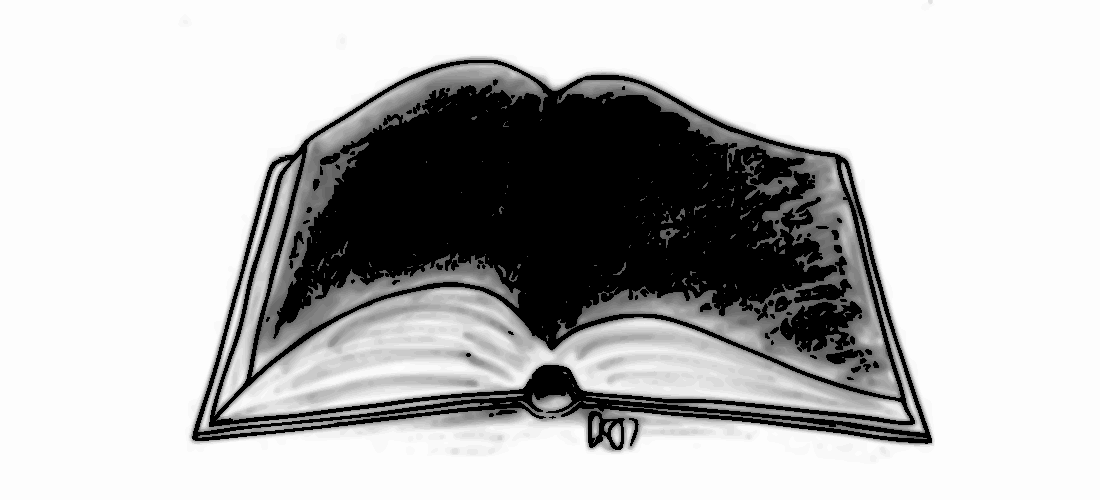
\includegraphics[width=\columnwidth]{vacuous.pdf}\label{vacuous}

\subsection{MAGICAL BOOKS \& TOMES}

\index{Wondrous Items!Books \& Tomes}This category includes books, librams, manuals, tomes, and an accursed grimoire.  Magical spell books are included, but not ordinary ones.  To generate an ordinary spell book refer to spell scrolls and wizard spell books.  Except for the blessed book (which appears to be a traveling spell book) and the book of infinite spells (which appears to be a standard spell book or other book of arcane lore), all other magical books, librams, manuals and tomes share several common traits.  They are crafted to appear to be mundane books of knowledge (refer to Commodities, Mundane Books) with heavy covers, and are usually bound in common leather and metal such as iron, silver, or brass.  Unless otherwise stated, no magical power or ability short of a \textit{wish} spell can determine that they are magical.  A single \textit{wish} spell will reveal that the book is magical and which character class or ability score will be most affected by reading the book.  A second \textit{wish} is required to determine the book's precise powers.

Any creature can read (or attempt to read) a magical book, even if ordinarily illiterate.  In addition to any negative effects listed in its individual description, the GM may determine that the book does not vanish but rather binds itself to the restricted reader making the attempt.  The book then acts as an accursed item, and the reader will be unable to get rid of it; throwing it away or destroying it causes it to reappear in the his possession.  In addition, if a book is restricted to specific alignments, a restricted reader may act as if affected by a \textit{geas} spell to keep the book safely hidden and protected. The GM must adjudicate the results of a restricted reader attempting to read a magical book using these rules as guidelines.

A character of the proper class and alignment must study the entire contents of the book to receive any benefits.  When he has finished reading, the book vanishes.  A reader can benefit from a specific magical book only once in his lifetime, even if he were to discover another of the same type.

\noindent
\begin{minipage}{\columnwidth}

\captionof{table}{Books and Tomes}\label{bookstomes}
\noindent
\begin{tabular}{|p{.1\columnwidth}|p{.6\columnwidth}|p{.15\columnwidth}|}
\hline
1d20	& Item	& XP \\
\hline\hline
\rowcolor[gray]{.9}1--3	& Blessed Book (Wizard)	& 4,500 \\
4	& Book of Infinite Spells	& 9,000 \\
\rowcolor[gray]{.9}5	& Book of Malevolent Deeds (Priest)	& 8,000 \\
6	& Book of Righteous Service (Priest)	& 8,000 \\
\rowcolor[gray]{.9}7	& Libram of Gainful Conjuration (Wizard)	& 8,000 \\
8	& Libram of Ineffable Damnation (Wizard)	& 8,000 \\
\rowcolor[gray]{.9}9	& Libram of Silver Magic (Wizard)	& 8,000 \\
10	& Manual of Agility	& 5,000 \\
\rowcolor[gray]{.9}11	& Manual of Battle Skills (Warrior/Rogue)	& 5,000 \\
12	& Manual of Bodily Health	& 8,000 \\
\rowcolor[gray]{.9}13	& Manual of Gainful Exercise	& 5,000 \\
14	& Manual of Golems (Priest/Wizard)	& 3,000 \\
\rowcolor[gray]{.9}15	& Manual of Surreptitious Burglary (Rogue)	& 8,000 \\
16	& Tome of Clear Thought	& 8,000 \\
\rowcolor[gray]{.9}17	& Tome of Leadership and Influence	& 7,500 \\
18	& Tome of Understanding	& 8,000 \\
\rowcolor[gray]{.9}19	& Vacuous Grimoire	& Accursed \\
20	& GM's Choice	& -- \\
\hline
\end{tabular}

\end{minipage}

\paragraph{Blessed Book:} These magical traveling spell books are of great benefit to one of the wizard class, including specialist mages.  They are well crafted, durable, and waterproof.  They are between 6 and 12 inches tall, 3 to 6 inches wide and about an inch thick.  Crafted of supple leather, bound with iron overlaid with silver, and locked, these books gain a +3 bonus to any item saving throw it makes.  The book magically creates enough pages to store up to a 45 spells regardless of the spell's level.

\paragraph{Book of Infinite Spells:} These magical standard-sized spell books contain collections of randomly generated spells.  The book's enchantment is such that any creature may cast the spells held in its pages.  When first found, the book cannot be opened to any but the title page.  Any creature is able to read this book, even if normally unable to read.  However, upon first reading the title page, any non-spell caster immediately suffers 5d4 points of damage and is stunned for 5d4 turns.  The pages can only be turned one at a time thereafter, and cannot be turned back.  Once opened past the title page, the book will only open to the current page.  Its owner is not aware of what spells lie on the pages ahead, and when the last page is turned, the book vanishes.  After the initial stun effect has passed, the non-spell caster can use the book with no further ill effects, but not as effectively as a spell caster.

Each book contains 22~+~1d8 pages.  Each page may be blank, or it may contain one spell from either the mage or priest lists, as shown on the table.  Each is rolled separately.

\noindent
\begin{tabular}{|p{.3\columnwidth}|p{.6\columnwidth}|}
\hline
1d100	& Page \\
\hline\hline
\rowcolor[gray]{.9}01-30	& Blank \\
31-60	& Priest spell \\
\rowcolor[gray]{.9}61-00	& Wizard spell \\
\hline
\end{tabular}

If a page contains a priest spell, roll 1d10 to determine its level, but if a result between 8 and 10 is rolled, roll 1d6 instead.  If a page contains a wizard spell, roll 1d12 to determine its level, but if a result between 10 and 12 is rolled, roll 1d8 instead.  The GM must secretly determine the content of each page by selecting or randomly determining the spell based on class and spell level.

The caster level of each spell within the book is the same as a comparable spell scroll and casting spells from a page is otherwise treated as if casting from a spell scroll, including the chance for spell failure.  

To function, the book must be open to a page containing a spell.  A spell caster that is normally able to cast the spell scribed on the exposed page can cast it up to four times per day, but all others are only able to cast it once per day.  The owner does not have to hold the book to cast the spell from the page.  It can be kept open in a safe place and will transmit the contents of the page to its owner as needed.  
 
The owner can physically turn the page whenever he desires.  In addition, there's a chance that the page may magically turn each time the spell on the current page is cast, as shown on the table below.  If the page turns to a page that is not blank, the owner is instantly aware of the new spell available.

\noindent
\begin{tabular}{|p{.75\columnwidth}|p{.15\columnwidth}|}
\hline
Status of Owner	& Chance \\
\hline\hline
\rowcolor[gray]{.9}Spell caster casting a known spell	& 10\% \\
Spell caster casting a spell not known to them	& 20\% \\
\rowcolor[gray]{.9}Non-spell caster casting priest spell	& 25\% \\
Non-spell caster casting wizard spell	& 30\% \\
\hline
\end{tabular}

\paragraph{Book of Malevolent Deeds:} This magical book is overflowing with knowledge of unspeakable evil that can only benefit an evil cleric.  Such a cleric who studies the book for one week gains one point of wisdom, a level of experience, and enough additional experience points to place him halfway to the level beyond that.  The book vanishes after the week of study.

If a neutral priest reads even a single word of this book, the book vanishes, and the priest is 50\% likely to either immediately become evil or lose 3d4~$\times$~10,000 xp.  A \textit{restoration} spell will restore these lost experience points and levels (if any).

If a good priest reads even a single word of this book, the book vanishes, and the priest must save vs. poison or die.  Those that make a successful save vs. poison must then save vs. spell or become irrevocably insane.  Those that make a successful save vs. spell will instead lose 250,000 xp minus 10,000 xp per point of wisdom.  A \textit{restoration} spell will restore these lost experience points and levels (if any).

The book inflicts 5d6 points of damage to any other good aligned creature that simply touches it.  If any other good aligned creature reads even a single word, the book vanishes and there is an 80\% chance that the creature becomes the victim of a night hag attack that night.

The book inflicts 5d4 points of damage to any other neutrally aligned creature that simply touches it.  If any other neutrally aligned creature reads even a single word, the book vanishes and the creature must make a successful save vs. poison or become evil.  Those that become evil will immediately seek out an evil priest to gain acceptance to their new alignment.

\paragraph{Book of Righteous Service:} This magical book imparts understanding of glorious actions that can only benefit a good cleric.  Such a cleric who studies the book for one week gains one point of wisdom, a level of experience, and enough additional experience points to place him halfway to the level beyond that.  The book vanishes after the week of study.

If a neutral priest reads even a single word of this book, the book vanishes, and the priest is 50\% likely to either immediately become good or lose 2d4~$\times$~10,000 xp.  A \textit{restoration} spell will restore these lost experience points and levels (if any).  A bard is treated as if he were a neutral priest.

If an evil priest reads even a single word of this book, the book vanishes, and the priest loses one level and enough additional experience points to place him at the lowest possible experience point total of the new level.  A \textit{restoration} spell will restore these lost experience points and level.  In addition, the evil priest must submit to an \textit{atonement} spell or willingly sacrifice 50\% of any treasure they find during their next 1d4~+~1 adventures to their patron deity.

If a wizard reads even a single word of this book, the book vanishes.  The wizard must successfully save vs. spell or lose one point of intelligence and 2d10~$\times$~1,000 xp.  A \textit{restoration} spell will restore these lost experience points and levels (if any).  

If a thief simply touches the book, the book vanishes and the thief immediately suffers 5d6 points of damage.  He must also save vs. spell or lose one point of dexterity.  If his wisdom is higher than 14, there is a (1d6~$-$~1)~$\times$~10\% chance (minimum of 10\%) to change his alignment to good (if not already good-aligned) and change his class to cleric (treat this as dual classing even if the thief is not a human).  

Any warrior can touch and even read from the book, but neither gains any benefits nor suffers any ill effects.  If the warrior is a paladin, he will be able to determine that the book is a good aligned, magical item.  Since the book has no effect on warriors, the GM must determine whether the book would normally vanish after being read by one.  This decision may be influenced by the warrior's alignment.

\paragraph{Libram of Gainful Conjuration:} This magical libram only benefits neutrally aligned wizards, including specialist mages.  When studied for one a week, the wizard gains one level and enough experience points to place him halfway to the level beyond that.  The libram vanishes after the week of study.

If any non-neutral wizard reads even a single word from this libram, it vanishes and the wizard suffers 5d4 hit points of damage.  The wizard then falls unconscious for the same number of turns and gains no more experience points until he submits to an \textit{atonement} spell.  

If any creature that is not a wizard reads even a single word from the libram, the libram vanishes and the creature must save vs. spell or go permanently insane.  A \textit{heal} spell or a \textit{remove curse} spell followed by a month of complete rest will cure a creature driven insane.

\paragraph{Libram of Ineffable Damnation:} This magical libram only benefits evil aligned wizards, including specialist mages.  When studied for one a week, the wizard gains one level and enough experience points to place him halfway to the level beyond that.  The libram vanishes after the week of study.  

If a non-evil wizard so much as opens the book, he loses one level of experience and enough experience points to place him halfway to the level just lost.  A \textit{restoration} spell will restore these lost experience points and level.  If he reads even a single word from this libram, it vanishes and the wizard suffers 5d4 hit points of damage.  The wizard then falls unconscious for a like number of turns and gains no more experience points until he submits to an \textit{atonement} spell.  

If any creature that is not a wizard reads even a single word from the libram, the libram vanishes and the creature must save vs. spell or go permanently insane.  A \textit{heal} spell or a \textit{remove curse} spell followed by a month of complete rest will cure a creature driven insane.

\paragraph{Libram of Silver Magic:} This magical libram only benefits good aligned wizards, including specialist mages.  When studied for one a week, the wizard gains one level and enough experience points to place him halfway to the level beyond that.  The libram vanishes after the week of study.

If any non-good wizard reads even a single word from this libram, it vanishes and the wizard suffers 5d4 hit points of damage.  The wizard then falls unconscious for the same number of turns and gains no more experience points until he submits to an \textit{atonement} spell.  

If any creature that is not a wizard reads even a single word from the libram, the libram vanishes and the creature must save vs. spell or go permanently insane.  A \textit{heal} spell or a \textit{remove curse} spell followed by a month of complete rest will cure a creature driven insane.

\paragraph{Manual of Agility:} This magical manual radiates magic if \textit{detect magic} is cast and will benefit any creature that reads it.  The manual provides temporary knowledge of inexpensive alchemical recipes to create secret ointments, as well as specific exercises designed to hone one's reflexes.  If a creature studies the manual for three uninterrupted days, the manual vanishes, but the creature retains the knowledge for up to three months thereafter.  If the one who reads the manual then spends one uninterrupted month diligently following the manual's instructions, he permanently gains 1 point of dexterity and the knowledge is lost.  No part of the manual can be copied or recorded in any way, nor can its secrets be spoken to others.  

\paragraph{Manual of Battle Skills:} This magical manual radiates magic if \textit{detect magic} is cast but will benefit only fighters and bards who read it.  Paladins and rangers may read it but gain no benefit or ill effect.  The manual provides expert advice on combat tactics.  If a fighter or bard studies the manual for three uninterrupted days, the manual vanishes, but the character retains the knowledge for up to three months thereafter.  If the one who reads the manual then spends one uninterrupted month diligently following the manual's instructions, he permanently gains one level and enough experience points to place him halfway to the level beyond that.  The knowledge is then lost.  No part of the manual can be copied or recorded in any way, nor can its secrets be spoken to others.  

Priests and thieves are not able to read the manual but suffer no ill effect from making the attempt.  However, a wizard who reads even a single word from this manual is stunned for 1d6 turns and lose 1d6~$\times$~10,000 experience points.  A \textit{restoration} spell will restore these lost experience points and levels (if any).  The GM must decide whether the manual vanishes when read by one other than a fighter or bard.

\paragraph{Manual of Bodily Health:} This magical manual radiates magic if \textit{detect magic} is cast and will benefit any creature that reads it.  The manual provides temporary knowledge of a special diet, as well as specific breathing exercises designed to increase one's stamina.  If a creature studies the manual for 24 hours within a period of five days, the manual vanishes, but the creature retains the knowledge for up to three months thereafter.  If the one who reads the manual then spends one uninterrupted month diligently following the manual's instructions, he permanently gains 1 point of constitution and the knowledge is lost.  No part of the manual can be copied or recorded in any way, nor can its secrets be spoken to others.  

\paragraph{Manual of Gainful Exercise:} This magical manual radiates magic if \textit{detect magic} is cast and will benefit any creature that reads it.  The manual provides temporary knowledge of a special diet, as well as specific muscle building exercises designed to increase one's physical power.  If a creature studies the manual for 24 hours within a period of up to five days, the manual vanishes, but the creature retains the knowledge for up to three months thereafter.  If the one who reads the manual then spends one uninterrupted month diligently following the manual's instructions, he permanently gains 1 point of strength and the knowledge is lost.  No part of the manual can be copied or recorded in any way, nor can its secrets be spoken to others.  

\paragraph{Manual of Golems:} These magical manuals are crafted in four known varieties.  Each is a collection of writings that when taken as a whole provides the designs and formulae required to construct a specific type of golem.  Due to the nature of the golem to be produced, most of these manuals are usable only by wizards, including specialty mages, but one is usable only by a priest.  The wizard or priest is first instructed to purchase rare and expensive materials.  Construction of the golem's physical form can then commence, so long as the construction time will not be interrupted and the caster keeps the manual on hand during the entire construction time.  By rolling 1d20 and consulting the table below, the GM may determine which manual has been found.  The GM may also expand this table as desired by adding new types of golems.
 
\noindent
\begin{tabular}{|p{.12\columnwidth}|p{.28\columnwidth}|p{.2\columnwidth}|p{.2\columnwidth}|}
\hline
1d20	& Type	& Time	& Cost \\
\hline\hline
\rowcolor[gray]{.9}1--5	& Clay (Priest)	& 1 month	& 65,000 gp \\
6--17	& Flesh (Wizard)	& 2 months	& 50,000 gp \\
\rowcolor[gray]{.9}18	& Iron (Wizard)	& 4 months	& 100,000 gp \\
19--20	& Stone (Wizard)	& 3 months	& 80,000 gp \\
\hline
\end{tabular}

The manual itself becomes the final component, for once the golem's physical form has been constructed, the manual bursts into flames and is consumed to ash.  Its ashes are sprinkled onto the golem, finalizing the process and animating the golem.  If the caster is 10\textsuperscript{th} level or higher, proper construction and successful animation is assured.  However, there's a 10\% chance per level of experience below 10th that the golem will fail one turn after being animated, collapsing into a pile of useless rubble.

If a priest reads even a single word from a wizard's manual, he loses 1d6~$\times$~10,000 experience points, and if a wizard reads even a single word from a priest's manual, he loses one level of experience and enough experience points to place him halfway to the level just lost.  In either case, a \textit{restoration} spell will restore these lost experience points and/or levels.  Other creatures that so much as open any of these manuals suffer 6d6 points of damage.

\paragraph{Manual of Surreptitious Burglary:} This magical manual radiates magic if \textit{detect magic} is cast but will benefit only rogues who read it.  The manual is a guide to thievery and subterfuge.  If a rogue studies the manual for three uninterrupted days, the manual vanishes, but the character retains the knowledge for up to three months thereafter.  If the one who reads the manual then spends one uninterrupted month diligently following the manual's instructions, he permanently gains one level and enough experience points to place him halfway to the level beyond that.    The knowledge is then lost.  No part of the manual can be copied or recorded in any way, nor can its secrets be spoken to others.

Fighters and wizards are not able to read the manual but suffer no ill effects from making the attempt.  However, a priest, ranger, or paladin who reads even a single word from this manual immediately suffers 5d4 points of damage and is stunned for a like number of rounds.  They must also make a successful saving throw vs. spell or lose 5d4~$\times$~10,000 experience points and unless they then submit to an \textit{atonement} spell within one day, they will permanently lose one point of wisdom.  A \textit{restoration} spell will restore these lost experience points and levels (if any).  The GM must determine whether the manual vanishes when read by one other than a rogue.

\paragraph{Tome of Clear Thought:} This magical tome will benefit any creature that reads it.  The tome provides temporary knowledge of specific mental exercises designed to increase one's higher brain functions.  If a creature studies the manual for 48 hours within a period of up to six days, the tome vanishes, but the creature retains the knowledge for up to one month thereafter.  

If the one who reads the manual then spends one uninterrupted week diligently following the tome's instructions, he permanently gains 1 point of intelligence and the knowledge is lost.  No part of the manual can be copied or recorded in any way, nor can its secrets be spoken to others.

\paragraph{Tome of Leadership and Influence:} This magical tome will benefit any creature that reads it.  The tome provides temporary knowledge of specific rules of poise, language and etiquette designed to increase one's personal appeal.  If a creature studies the manual for 48 hours within a period of up to six days, the tome vanishes, but the creature retains the knowledge for up to one month thereafter.  If the one who reads the manual then spends one uninterrupted week diligently following the tome's instructions, he permanently gains 1 point of charisma and the knowledge is lost.  In addition, if a bard reads the tome, he also gains enough experience points to achieve the minimum experience required to gain his next level.  No part of the manual can be copied or recorded in any way, nor can its secrets be spoken to others.

\paragraph{Tome of Understanding:} This magical tome will benefit any creature that reads it.  The tome provides temporary knowledge of specific meditation techniques designed to increase one's ability to make common sense decisions.  If a creature studies the manual for 48 hours within a period of up to six days, the tome vanishes, but the creature retains the knowledge for up to one month thereafter.  If the one who reads the manual then spends one uninterrupted week diligently following the tome's instructions, he permanently gains 1 point of wisdom and the knowledge is lost.  No part of the manual can be copied or recorded in any way, nor can its secrets be spoken to others.

\paragraph{Vacuous Grimoire:} This accursed grimoire radiates magic if \textit{detect magic} is cast, but any creature that reads even a single word must make two successful saving throws vs. spell.  Failing the first results in a permanent loss of one point of intelligence.  Failing the second results in a permanent loss of two points of wisdom.  The grimoire is further cursed so that when it is placed on a shelf with other books, it instantly shuffles itself to a different location on the shelf and changes its appearance to look like the book whose place it now occupies.  Only by setting it alight while casting a \textit{remove curse} spell upon it can the grimoire be destroyed.

\subsection{JEWELS \& JEWELRY}

\index{Wondrous Items!Jewels \& Jewelry}This category includes magical items in the form of ordinary raw gemstones and jewelry that in many cases will be crafted to include precious metals and one or more gemstones.  Unless otherwise stated in their descriptions, the gems can either be cut smoothly (cabochon) or be faceted.  The GM should consult the sections on mundane jewelry and gemstones as needed to determine the appearance of magical jewelry.  He should avoid including pearls as they are listed separately. 

A magical amulet can be suspended on a chain and worn around the owner's neck.  Its owner can hang it from any type of mundane chain, ranging from leather to finely wrought platinum, as the chain is completely unrelated to the amulet's powers.  An amulet can also be pinned to its owner's shirt, cloak or even headwear, but will not function if worn on his boot or glove.  No creature may wear more than two amulets at the same time, one around its neck and one on its clothing.

A magical brooch is similar to an amulet but only functions when worn on the owner's clothing.

A magical medallion is similar to an amulet but only functions when worn around the owners' neck upon a mundane chain.

A magical necklace is similar to an amulet worn around the neck, but its chain is related to its powers and cannot be replaced.

A magical periapt is an unadorned gemstone.  Other than its unusually large size, a periapt is indistinguishable from any other magical gem or \textit{ioun stone}, but like an amulet must be worn upon a garment or hung around the owner's neck in order to function.

A magical phylactery is similar to an amulet, but contains a tiny prayer book and can be worn on the forehead, wrist, upper arm or thigh. 

A scarab is a specific type of amulet almost always crafted in the form of a dung beetle, which can be worn around the neck or on the clothing.  Even if not originally crafted in this form, a scarab will transform into beetle form when activated.

A talisman is similar to both an amulet and phylactery and can be worn around the neck, forehead, wrist, arm, thigh, or on the clothing.

\noindent
\begin{minipage}{\columnwidth}

\captionof{table}{Jewelry \& Jewels (1d6)}\label{jewelsa}
\noindent
\begin{tabular}{|p{.1\columnwidth}|p{.5\columnwidth}|p{.25\columnwidth}|}
\multicolumn{3}{c}{Sub-Table A (1--3)} \\
\hline
1d20	& Item	& XP \\
\hline\hline
\rowcolor[gray]{.9}1	& Amulet of Inescapable Location	& Accursed \\
2	& Amulet of Life Protection	& 5,000 \\
\rowcolor[gray]{.9}3	& Amulet of the Planes	& 6,000 \\
4	& Amulet of Warding	& 4,000 \\
\rowcolor[gray]{.9}5	& Amulet vs. Undead	& 200/effective level or HD \\
6	& Beads of Force	& 200/bead \\
\rowcolor[gray]{.9}7	& Brooch of Shielding	& 1,000 \\
8	& Gem of Brightness	& 2,000 \\
\rowcolor[gray]{.9}9	& Gem of Insight	& 3,000 \\
10	& Gem of Seeing	& 2,000 \\
\rowcolor[gray]{.9}11	& Jewel of Attacks	& Accursed \\
12	& Jewel of Flawlessness	& -- \\
\rowcolor[gray]{.9}13	& Medallion of ESP	& 2,000 \\
14	& Medallion of Thought Projection	& -- \\
\rowcolor[gray]{.9}15	& Necklace of Adaption	& 1,000 \\
16--17	& Necklace of Missiles	& 100/die of damage \\
\rowcolor[gray]{.9}18	& Necklace of Prayer Beads (Priest)	& 500/bead \\
19	& Necklace of Strangulation	& Accursed \\
\rowcolor[gray]{.9}20	& GM's Choice	& -- \\
\hline
\end{tabular}

\end{minipage}

\noindent
\begin{tabular}{|p{.09\columnwidth}|p{.6\columnwidth}|p{.16\columnwidth}|}
\multicolumn{3}{c}{Sub-Table B (4--6)} \\
\hline
1d20	& Item	& XP \\
\hline\hline
\rowcolor[gray]{.9}1	& Pearl of Power (Wizard)	& 200/level \\
2	& Pearl of the Sirens	& 900 \\
\rowcolor[gray]{.9}3	& Pearl of Wisdom (Priest)	& 500 \\
4	& Periapt of Foul Rotting	& Accursed \\
\rowcolor[gray]{.9}5	& Periapt of Health	& 1,000 \\
6	& Periapt of Proof Against Poison	& 1,500 \\
\rowcolor[gray]{.9}7	& Periapt of Wound Staunching	& 1,000 \\
8	& Phylactery of Faithfulness (Priest)	& 1,000 \\
\rowcolor[gray]{.9}9	& Phylactery of Long Years (Priest)	& 1,000 \\
10	& Phylactery of Monstrous Attention (Priest)	& Accursed \\
\rowcolor[gray]{.9}11	& Scarab of Death	& Accursed \\
12	& Scarab of Enragement	& 1,000 \\
\rowcolor[gray]{.9}13	& Scarab of Insanity	& 1,500 \\
14	& Scarab of Protection	& 2,500 \\
\rowcolor[gray]{.9}15	& Scarab vs. Golems	& See description \\
16	& Talisman of Pure Good (Priest)	& 3,500 \\
\rowcolor[gray]{.9}17	& Talisman of the Sphere (Wizard)	& 100 \\
18	& Talisman of Ultimate Evil (Priest)	& 3,500 \\
\rowcolor[gray]{.9}19	& Talisman of Xagy Gyrag	& 1,000 \\
20	& GM's Choice	& -- \\
\hline
\end{tabular}

\paragraph{Amulet of Inescapable Location:} This accursed amulet deludes its wearer into believing that it is an \textit{amulet of proof against detection and location}.  In reality, this amulet doubles the range and duration of all scrying or other divination effects attempted upon the wielder or amulet.  The amulet can be removed normally, however the wearer will resist doing so unless the GM allows him to disbelieve the delusion.

\paragraph{Amulet of Life Protection:} Primarily, this magical amulet protects its wearer from \textit{magic jar} effects and any other attacks that attempt to take control or possess the wielder's body.  In addition, if its wearer would ordinarily be slain, his life force enters the amulet and his body (if it still exists) enters a form of \textit{temporal stasis} and will not truly die for up to seven days.  If magical healing is employed to increase the body's hit points above zero within those seven days, the life force leaves the amulet and re-enters the body.  

If its wearer was to be irrevocably slain or his body completely destroyed, the power of the amulet allows its wearer to be affected by a \textit{raise dead} or \textit{resurrection} (as applicable) normally within those seven days.  In any case, if the amulet is destroyed within those seven days, the wearer's life force is irrevocably lost and he cannot be raised from the dead by any method.  If seven days pass uneventfully, the wearer dies in whatever way he initially would have been slain (both his body and life force).  

\paragraph{Amulet of the Planes:} This extremely powerful magical amulet enables its wearer to be transported instantly and safely to or from the upper layer of any Outer Plane of the wearer's choice as if a \textit{plane shift} spell had been cast.  However, if its wearer activates the amulet without knowledge of its power, he's transported to a randomly determined plane.  Roll 1d12 and consult the following table.

\noindent
\begin{tabular}{|p{.3\columnwidth}|p{.6\columnwidth}|}
\hline
1d12	& Plane \\
\hline\hline
\rowcolor[gray]{.9}1	& Astral Plane \\
2	& Ethereal Plane \\
\rowcolor[gray]{.9}3	& Alternate Prime Material \\
4	& Lawful Good Plane \\
\rowcolor[gray]{.9}5	& Lawful Neutral Plane \\
6	& Lawful Evil Plane \\
\rowcolor[gray]{.9}7	& Neutral Good Plane \\
8	& Neutral Plane \\
\rowcolor[gray]{.9}9	& Neutral Evil Plane \\
10	& Chaotic Good Plane \\
\rowcolor[gray]{.9}11	& Chaotic Neutral Plane \\
12	& Chaotic Evil Plane \\
\hline
\end{tabular}

Even when the amulet's power is known, the GM may require its wearer to roll a successful intelligence check, with a $-4$ or higher penalty, each time its power is activated to avoid being randomly transported and arrive at the desired plane.

\noindent
\includegraphics[width=3.6in, height=1in]{testblock.pdf}

\paragraph{Amulet of Proof Against Detection and Location:} This magical amulet protects its wearer against any and all divination, location and detection effects, including, but not limited to \textit{clairaudience}, \textit{clairvoyance}, \textit{ESP}, and \textit{crystal balls}.  It also masks the wearer's auras and clouds any predictions regarding his actions unless an artifact, relic or creature of demigod status or higher is consulted.

\paragraph{Amulet Versus Undead:} When this magical amulet is presented strongly in the presence of the undead, it begins to glow, enabling its wearer to turn undead as if he were a cleric of a level determined by the amulet's strength.  This amulet is powerless until a single creature has worn it for at least seven days.  Each time it is removed from its wearer's neck, it becomes temporarily powerless until worn again for another seven days (even if worn by the same creature).  They are crafted in five known strengths.  The GM may roll randomly to determine a particular amulet's strength by rolling 1d100 and consulting the following table.

\noindent
\begin{tabular}{|p{.3\columnwidth}|p{.6\columnwidth}|}
\hline
1d100	& Strength \\
\hline\hline
\rowcolor[gray]{.9}01--30	& 5\textsuperscript{th} level \\
31--55	& 6\textsuperscript{th} level \\
\rowcolor[gray]{.9}56--75	& 7\textsuperscript{th} level \\
76--90	& 8\textsuperscript{th} level \\
\rowcolor[gray]{.9}91--00	& 9\textsuperscript{th} level \\
\hline
\end{tabular}

The amulet's experience point value is equal to 200 times its effective clerical level.

\paragraph{Beads of Force:} These magical beads are usually crafted from solid black glass, ceramic, metal or similar material, $^3$/$_4$ of an inch in diameter, and weigh 0.1 pound each.  They are found singly or in small groups (of d4~+~4) strung onto a mundane string.  They can be hurled up to 30 yards away, ignoring range and combat skill penalties, and burst upon impact, inflicting 5d4 points of damage to all creatures within a 10-foot radius.  Large-sized or smaller creatures may also be trapped inside an impenetrable sphere of force (refer to \textit{wall of force}) for 3d4 rounds.  A successful saving throw vs. spell reduces the damage by half and moves the creature to the outside edge of the sphere.

\paragraph{Brooch of Shielding:} This magical brooch is crafted in either silver or gold but only rarely (10\%) holds gemstones.  When it is used to fasten a cloak or cape, it absorbs all \textit{magic missiles} that target its wearer, rendering them harmless.  The brooch is initially crafted with 101 charges.  The brooch expends one charge for every hit point of \textit{magic missile} damage absorbed (whether from spell, magical item or spell-like ability), and crumbles to dust when the last charge is expended.

\paragraph{Gem of Brightness:} This magical gemstone appears to be any faceted crystal that has been cut into a long, somewhat uneven prism.  The gem is initially crafted with 50 charges and cannot be recharged.  The gem has three distinct powers, each activated by a separate command word or phrase, spoken while the gem is held in the owner's hand and pointed towards its target.

\underline{Lantern's light:} When this power is activated, the gem shines a pale beam of light in a 10-foot long, 2$^1$/$_2$-foot wide cone.  This power does not expend a charge.

\underline{Dazzling light:} When this power is activated, the gem shines a bright ray of light, 50 feet long with a 1-foot diameter.  The creature targeted by the ray must roll a successful save vs. spell or be blinded for 1d4 rounds.  This power expends one charge.  The blindness that it causes can be cured by a \textit{cure blindness or deafness} spell.

\underline{Blinding light:} When this power is activated, the gem shines a blinding flash of light in a 30-foot long, 5-foot wide cone.  All creatures in the effective area must roll a successful save vs. spell or be blinded for 1d4 rounds and thereafter suffer up to a $-4$ penalty to attack rolls due to permanent damage to the creatures' eyes (roll 1d4 to determine the penalty).  The blindness caused by this power can be cured by a \textit{cure blindness or deafness} spell, but the permanent eye damage can only be cured by a \textit{heal} spell.  This power expends 5 charges.

In addition, the gem is sensitive to \textit{darkness} and \textit{continual darkness} spells that target its owner.  If \textit{darkness} is cast upon the gem's owner, the gem becomes inactive for one round unless the owner chooses to expend one charge.  If \textit{continual darkness} is cast upon the gem's owner, the gem becomes inactive for one day unless the owner chooses to expend 5 charges.

\paragraph{Gem of Insight:} This magical gemstone appears to be any valuable and expertly cut stone worth at least 5,000 gp.  However, if a \textit{detect magic} spell is successfully cast upon it, the gem radiates a faint aura of enchantment.  

This gem is powerless until a single creature has carried it for at least seven days, whereupon the gem's owner feels its power begin to build.  If the same creature carries the gem for three continuous months, that creature's intelligence and wisdom scores are increased by one point each.  If the owner stops carrying the gem for any reason after the three month period the extra point of wisdom is lost, but the intelligence remains.

Each gem functions for only a single creature, once every 50 years.  A creature can never benefit from this type of gem more than once, even if he has only gained the extra point of intelligence and lost the point of wisdom gained from the first one.

\paragraph{Gem of Seeing:} This magical gemstone appears to be any valuable and expertly cut faceted stone worth at least 5,000 gp.  However, if a \textit{detect magic} spell is successfully cast upon it, the gem radiates a moderately strong aura of divination.  The gem's power shares some similarities to the effects of a \textit{true seeing} spell and has the same limitations.  In many cases, activating the gem substitutes for the casting of the spell.  

To activate the gem, its owner (or other creature) simply gazes through one of its facets.  When activated, the gem may reveal hidden, illusory, invisible, astral, ethereal, or out-of-phase objects or creatures that are within its viewing range.  The creature gazing through the gem can see out to a range of up to 300 feet.  

Gazing through the gem can be compared to looking through a spyglass.  Any creature who gazes through the gem can detect large-sized or larger creatures and objects within 300 feet straight ahead after less than one round of viewing, those that are man-sized or larger within 200 feet straight ahead after 1 full round of viewing, those that are small-sized or larger within 100 feet straight ahead after 2 full rounds of viewing, and those that are tiny-sized or larger within 50 feet straight ahead after 3 full rounds of viewing.  

Each time the gem is used there's a 5\% chance that the viewer will see something that's not really there or a real creature or object will appear to be illusory.

\paragraph{Jewel of Attacks:} This accursed jewel appears to be any valuable and expertly cut stone worth at least 5,000 gp.  However, if a \textit{detect magic} spell is successfully cast upon it, the jewel radiates an aura of enchantment.  The first creature to pick up the jewel becomes its owner.  The jewel's power immediately doubles the chances of its owner encountering wandering monsters, and if its owner wishes to flee the encounter, the chances of being chased are also doubled.  

The owner cannot be rid of the jewel by any means and the gem will always return to the owner's possession until a \textit{remove curse} spell or \textit{atonement} spell is cast on him.

\paragraph{Jewel of Flawlessness:} This magical jewel appears to be any valuable and expertly cut faceted stone worth at least 5,000 gp.  However, if a \textit{detect magic} spell is successfully cast upon it, the jewel radiates an aura of enchantment.  The jewel is initially crafted with 10d10 facets that correspond to its number of charges.  When placed among mundane gemstones, the power of the jewel gives each gem a 20\% chance to increase in value (refer to Gemstones).  If the jewel successfully increases the value of a gem, one of its facets vanishes.  The power of the jewel can affect a particular gemstone only once, whether the attempt is successful or not.  When all of its facets are gone, the jewel becomes a smooth, mundane rock of no value (similar to a sling stone).

\paragraph{Medallion of ESP:} This magical medallion is most commonly crafted from bronze, copper, or even cupronickel, set with only the most inexpensive ornamental gemstones (q.v., if any), and appears to be an inexpensive, mundane trinket.  However, if a \textit{detect magic} spell is successfully cast upon it, the jewel radiates an aura of divination.  The chain is not magical but should also be made of base metal as contact with silver, gold or platinum disrupts the medallion's powers.  To activate the medallion, the wearer must face the area to be scanned, grasp the medallion with one hand, and concentrate for at least one full round.  The medallion is crafted in four known varieties with different scanning ranges or abilities.  The GM may roll 1d20 to determine the type of medallion found.

\noindent
\begin{tabular}{|p{.2\columnwidth}|p{.7\columnwidth}|}
\hline
1d20	& Range \\
\hline\hline
\rowcolor[gray]{.9}1--15	& 30' long~$\times$~6' wide cone \\
16--18	& 30' long~$\times$~6' wide cone, plus empathy \\
\rowcolor[gray]{.9}19	& 60' long~$\times$~12' wide cone \\
20	& 90' long~$\times$~18' wide cone \\
\hline
\end{tabular}

The GM should roll 1d6 each round that the wearer uses the medallion's power, including the first.  If a 1 is rolled, the medallion fails to function that round.  Otherwise, the medallion allows its wearer to pick up surface thoughts of any creatures (except for the undead, the non-intelligent and the completely alien) within the effective area.  This also allows the wearer to note the creature's approximate distance.  In order to understand a creature's surface thoughts, the wearer must understand its primary language.  If the medallion has the power of empathy, the wearer can also learn the creature's emotional state (angry, happy, sad, etc.), even if the creature does not have a spoken language or if the wearer of the medallion does not speak its language.  The medallion's powers are blocked by at least 3 feet of stone, 2 inches of metal, or any amount of lead, gold, or platinum.  

\paragraph{Medallion of Thought Projection:} This accursed medallion has all of the properties of a \textit{medallion of ESP} in every way (including the four known varieties).  However, each round this medallion is used, it may also transmit its wearer's surface thoughts and/or emotions to all creatures within range unless the GM rolls a 1 on the d6 (indicating the medallion fails completely) or a 6 on the d6 (indicating the medallion only fails to transmit its wearer's thoughts).  The medallion can be removed at any time, however the wearer resists doing so unless the GM allows him to determine that his thoughts are being transmitted.

\paragraph{Necklace of Adaptation:} This magical necklace is commonly crafted as a chain of precious metals and gemstones with a matching medallion.  It has the power to render its wearer immune to any gas-borne effect that would affect him through breathing.  Its wearer can also breathe underwater indefinitely or exist in a vacuum for up to seven days at a time.

\paragraph{Necklace of Missiles:} This magical necklace is enchanted to appear to be made of bronze, copper, or even cupronickel, with one or more matching inexpensive medallions.  However, when worn around a creature's neck, that creature sees one or more golden spheres hanging upon a golden chain.  A sphere can be thrown up to 70 feet away, where it explodes into a fireball (refer to the \textit{fireball} spell).  Only the wearer of the necklace can detach and throw a sphere and suffers no range or combat skill penalties to do so.  This necklace is initially crafted with as few as 3 spheres or as many as 9 spheres of various strengths.   The GM may roll 1d20 and consult the table below, but if its previous owner(s) regularly employed the spheres, the number will be less when found.

More powerful spheres will be larger than those less powerful.  If its owner is wearing, holding or even carrying the necklace and fails a saving throw against a magical fire attack, the necklace must successfully save or all of its remaining spheres explode simultaneously.  Magical fire attacks that do not grant a saving throw will not generally cause the necklace to detonate except under special circumstances.

\paragraph{Necklace of Prayer Beads:} This magical necklace is enchanted to appear to be a mundane chain of colorful, but inexpensive, prayer beads made of ceramic and linked by a bronze, copper, or cupronickel chain.  However when worn around the neck of a cleric, he sees that the beads are gemstones, linked by gold.  The necklaces are crafted with 1d6~+~24 gemstones, 60\% of which will be semi-precious and 40\% will be fancy.  

In addition, each necklace holds 1d4~+~2 precious stones, gemstones and jewels with a value of at least 1,000 gp each.  These greater beads contain randomly determined powers.  The only way to determine the powers of the greater beads and how to activate them is to cast a commune spell upon each bead.  The necklace must be worn to activate any of its powers, and the power of a greater bead is lost if removed from the necklace.  Spell-like powers function as if cast by a 12\textsuperscript{th}  level caster.  The GM rolls 1d20 once for each greater bead and consults the following table.

\noindent
\begin{tabular}{|p{.15\columnwidth}|p{.75\columnwidth}|}
\hline
1d20	& Power \\
\hline\hline
\rowcolor[gray]{.9}1--5	& \textit{Atonement}, once per day. \\
6--10	& Bless, once per day. \\
\rowcolor[gray]{.9}11--15	& \textit{Cure blindness or deafness}, \textit{cure disease}, or \textit{cure serious wounds} once per day. \\
16--17	& All spells cast by the cleric function as if he was a caster of 4 levels higher.  Multiple beads don't stack. \\
\rowcolor[gray]{.9}18	& This bead grants the cleric a 90\% chance to successfully call upon his deity to come directly (or send an avatar) to his aid.  The deity will confiscate the necklace as the least punishment for improper or frivolous use of this power.  This bead functions once then becomes powerless. \\
19--20	& \textit{Wind walk} once per day. \\
\hline
\end{tabular}

If the GM desires, 75\% of all known necklaces of prayer beads radiate an aura of good, 20\% radiate neutral and 5\% radiate evil.  Unlike most other aligned magical items, the necklace inflicts no damage or loss of experience points to a character whose alignment does not match that of the beads.  However, the necklace will only function when worn by a cleric whose alignment does match.

\end{multicols}

\noindent
\begin{tabular}{|p{.14\textwidth}|p{.06\textwidth}|p{.06\textwidth}|p{.06\textwidth}|p{.06\textwidth}|p{.06\textwidth}|p{.06\textwidth}|p{.06\textwidth}|p{.06\textwidth}|p{.06\textwidth}|p{.06\textwidth}|}
\multicolumn{11}{c}{Necklace of Missiles: Number of Missiles and Damage Dice} \\
\hline
1d20	& 11d6	& 10d6	& 9d6	& 8d6	& 7d6	& 6d6	& 5d6	& 4d6	& 3d6	& 2d6 \\
\hline\hline
\rowcolor[gray]{.9}1--4	& -	& -	& -	& -	& -	& -	& 1	& -	& 2	& - \\
5--8	& -	& -	& -	& -	& -	& 1	& -	& 2	& -	& 2 \\
\rowcolor[gray]{.9}9--12	& -	& -	& -	& -	& 1	& -	& 2	& -	& 4	& - \\
13--16	& -	& -	& -	& 1	& -	& 2	& -	& 2	& -	& 4 \\
\rowcolor[gray]{.9}17--18	& -	& -	& 1	& -	& 2	& -	& 2	& -	& 2	& - \\
19		& -	& 1	& -	& 2	& -	& 2	& -	& 4	& -	& - \\
\rowcolor[gray]{.9}20		& 1	& -	& 2	& -	& 2	& -	& 2	& -	& 2	& - \\
\hline
\end{tabular}

\begin{multicols}{2}

\paragraph{Necklace of Strangulation:} This accursed necklace can be crafted from any combination of metal and/or gemstones and in any style.  It radiates magic if \textit{detect magic} is cast, but most common means of magical identification will not determine that it is cursed.  When placed around a creature's neck, the necklace immediately constricts around its throat, and the wearer of the necklace suffers 6 points of strangulation damage per round until he dies.  Only a \textit{limited wish} or \textit{wish} spell can remove the necklace from its victims neck.  Otherwise, the necklace remains clasped around the victim's neck until the body completely decomposes.  Removing the necklace from its wearer, either before or after death, does not destroy it.

\paragraph{Pearl of Power:} This magical pearl is only useful to a wizard, including any specialist mage.  Once per day, the pearl allows a wizard to recall one, or at most 2 spells, which he has already cast on that same day.  There are 10 known varieties, not including those cursed (see below).  More powerful pearls allow the caster to recall a spell of higher level or more than one spell.  The GM can roll 1d100 to determine which variety is found.  
 
\noindent
\begin{tabular}{|p{.2\columnwidth}|p{.7\columnwidth}|}
\hline
1d100	& Spell Level \\
\hline\hline
\rowcolor[gray]{.9}01--25	& 1\textsuperscript{st} \\
26--45	& 2\textsuperscript{nd} \\
\rowcolor[gray]{.9}46--60	& 3\textsuperscript{rd} \\
61--75	& 4\textsuperscript{th} \\
\rowcolor[gray]{.9}76--85	& 5\textsuperscript{th} \\
86--92	& 6\textsuperscript{th} \\
\rowcolor[gray]{.9}93--96	& 7\textsuperscript{th} \\
97--98	& 8\textsuperscript{th} \\
\rowcolor[gray]{.9}99 	& 9\textsuperscript{th} \\
00	& 2 spells of 1d6 level \\
\hline
\end{tabular}

It is known that 5\% of these pearls are cursed and cause one or more spells to be forgotten.  Determine an accursed pearl's power as above.  An accursed pearl remains in the wizard's possession and causes him to forget a spell of the specified level at the moment he tries to cast it.  If the caster has more than one spell of that level memorized, the GM should roll which spell will be affected in advance, but cannot reveal this to the player.  If the same spell is memorized more than once, each spell incurs an increasing chance to fail when cast until one casting finally fails.  For example: A wizard has a pearl that causes him to forget a third level spell each day, and he can normally cast four 3\textsuperscript{rd} level spells each day.  The wizard has memorized \textit{fireball} three times and \textit{lightning bolt} once.  Each distinct spell has a 50\% chance to be the one to be forgotten at casting time.  If \textit{fireball} is determined as the spell to be forgotten, it has a 33\% chance to fail on the first casting, 67\% chance to fail on the second and it will fail with 100\% certainty on the third casting.  The GM must predetermine which spell will be forgotten in this same manner each time one or more spells of the specified level are memorized.  Throwing away or destroying this accursed pearl causes it to reappear in the owner's possession.  Only a \textit{wish} spell allows it to be discarded successfully.  The pearl is not destroyed by this \textit{wish}.

\paragraph{Pearl of the Sirines:} This magical pearl is strikingly gorgeous and has a value of at least 1,000 gp.  It will radiate a faint aura of enchantment magic if a \textit{detect magic} is cast.  The pearl will communicate its powers to any creature that holds the pearl in its hand whilst underwater.  After that, as long as the owner is within 10 feet of the pearl, it grants him immunity to the poisonous touch of a sirine, as well as allows him to breathe water and to swim at double his normal movement value.

\paragraph{Pearl of Wisdom:} This magical pearl is only useful to priests, including druids.  If a priest carries this pearl on his person uninterrupted for 30 consecutive days, he gains 1 point of wisdom.  The owner must also carry the pearl with him at all times thereafter, or the point of wisdom is immediately lost.  He must carry the pearl for another 30 consecutive days to regain it. 

It is known that 5\% of these pearls are cursed.  After carrying the pearl for thirty days, the priest loses one point of wisdom and the pearl turns to dust.  The lost wisdom can only be restored by a \textit{wish}, a \textit{tome of understanding}, or divine intervention.

\paragraph{Periapt of Foul Rotting:} This accursed gem looks identical to a \textit{periapt of health}, but as soon as a creature claims ownership over the gem, the creature is inflicted with a foul, flesh rotting disease.  The owner does not have to wear the periapt for its curse to activate.  He can destroy or discard the gem, give it away or even try to sell it, but if another creature claims ownership of it, they too will unknowingly contract the disease.  Each week after claiming the gem (even if the creature no longer owns it), those afflicted lose one point of dexterity, constitution, and charisma, permanently.  If any of these scores reach zero, the victim dies.  The disease can be cured by a \textit{remove curse}, \textit{cure disease}, \textit{heal}, and \textit{limited wish} or \textit{wish}, cast in that order.  Crushing a periapt of health and sprinkling the dust on the victim can also cure the disease.

\paragraph{Periapt of Health:} This magical gem appears to be an ornamental or semi-precious stone (refer to Gemstones) of less than 50 gp value and is engraved with a well-known design or symbol indicating healing power such as a caduceus.  Wearing the periapt grants immunity to all diseases, except that which is spread by the \textit{periapt of foul rotting} or curse-diseases such as lycanthropy.

\paragraph{Periapt of Proof Against Poison:} This magical gem looks identical to a \textit{periapt of health}.  There are 4 known varieties of this periapt, as determined by rolling 1d20 and consulting the table below.  If a poison normally inflicts a penalty to the victim's saving throws, the wearer ignores those penalties.  If the poison grants a normal saving throw or one with bonuses, this gem grants its wearer an additional bonus (as shown on the table) and finally, the wearer is granted a special saving throw (as shown on the table) even if the poison doesn't normally allow a save, but no bonuses of any kind can be applied to this save.

\noindent
\begin{tabular}{|p{.25\columnwidth}|p{.3\columnwidth}|p{.3\columnwidth}|}
\hline
1d20	& Bonus	& Save \\
\hline\hline
\rowcolor[gray]{.9}1--8	& +1	& 19 \\
9--14	& +2	& 17 \\
\rowcolor[gray]{.9}15--18	& +3	& 15 \\
19--20	& +4	& 13 \\
\hline
\end{tabular}

\paragraph{Periapt of Wound Closure:} This magical gem looks identical to a \textit{periapt of health}.  When worn, it prevents wounds from bleeding, doubles the rate of natural healing, and allows wounds that ordinarily do not heal to be healed normally.

If worn while being attacked by a weapon such as a \textit{sword of wounding}, \textit{sword of sharpness} or \textit{vorpal blade}, this gem prevents its wearer from suffering additional damage each round from bleeding, as applicable.  The wearer continues to heal naturally at double the normal rate, even if struck by a \textit{sword of wounding}.  The GM may also determine that the gem allows magical healing of damage from a \textit{sword of wounding}.

\paragraph{Phylactery of Faithfulness:} The powers of this magical holy item cannot be discerned until any priest, including a druid, wears it, whereupon it immediately conforms to the priest's alignment.  When worn, this phylactery allows the priest to spend one round in meditation to determine if a proposed action or contact with an item (magical or otherwise) would adversely effect his alignment or anger his deity.

\paragraph{Phylactery of Long Years:} When worn by any priest, including a druid, this magical holy item slows his physical aging by one-quarter.  This reduction also applies to magical aging.  The character now has two effective ages, one physical and one mental.  As long as he wears the phylactery, he mentally ages as normal, but physically ages only 1 year for every 16 months.  It is known that 5\% of these phylacteries are cursed and increase physical aging, including magical aging, by one-quarter, so that its wearer physically ages 1 year every 9 months.  His mental aging remains at the same rate.  A \textit{remove curse} spell is required to remove the accursed phylactery.

\paragraph{Phylactery of Monstrous Attention:} When worn by a priest, including a druid, this accursed holy item announces his presence to any and all creatures from the Outer Planes that have an alignment directly opposite of his own.  This occurs whenever the priest is in an area where these creatures can normally be found.  Depending on their alignment and intelligence, these creatures will seek to attack, trick or otherwise harass the priest as soon as they have the opportunity.  The GM should determine which alignment, other than neutral, becomes hostile toward a neutral cleric or druid only once, when the phylactery is first put on.  If the priest is 10th level or higher when he puts on this phylactery, or he becomes 10\textsuperscript{th} level while wearing it, his presence will be announced to his deity's most powerful enemy.  This creature (most likely of demigod status or higher) will then become personally involved in assaulting or harassing the priest whenever possible.  The GM must determine the exact nature of this being's personal involvement, depending upon the creature's intelligence, powers, sphere of dominance, fear of reprisal from the priest's deity, etc.  This phylactery can only be removed by the casting of a \textit{wish} spell, immediately followed by a holy \textit{quest} designed to restore the priest's faith.  The character loses all of his priest abilities until he starts his \textit{quest}.
 
\paragraph{Scarab of Death:} Despite its name, this accursed scarab is crafted in the form of either an amulet or brooch of any style and manufacture, and is usually not crafted in the shape of a scarab beetle.  It radiates magic if \textit{detect magic} is cast, but most common means of magical identification will not determine that it is cursed.  If this scarab is held or worn for more than one round or is placed into any container made from leather, cloth, straw or other soft material within 1 foot of a living creature for one turn, the scarab transforms into a living, burrowing scarab beetle.

This beetle is able to tear through a soft container, get under a creature's armor (as applicable), burrow into his flesh, and eat his heart, automatically killing the creature in one full round.  It then returns to its original form, while still deep inside its victim's chest.  The missing heart will prevent a \textit{raise dead} spell from reviving the victim.  Quickly placing the scarab into a closed container made from solid wood, ceramic, bone, ivory, metal or other hard materials will prevent its transformation.

\paragraph{Scarab of Enraging Enemies:} This magical scarab is typically crafted with 1d6~+~18 charges, and each use of the scarab expends one charge.  When worn openly where it can be seen and a command spoken, this scarab causes all intelligent, hostile creatures within a 40-foot radius to save vs. spell or immediately enter a state of mind similar to berserk rage for 1d6~+~6 rounds.  Those who fail this save attack the nearest creature regardless of friend or foe, gaining a +1 bonus to attack, +2 bonus to damage, and a $-3$ penalty to AC.  While under this effect, the creature never checks morale and attacks only with melee weapons or natural weaponry (claws, teeth, etc.), mindlessly moving to attack another creature if the one it is currently attacking falls.

\paragraph{Scarab of Insanity:} This magical scarab is typically crafted with 1d8~+~8 charges, and each use of the scarab expends one charge.  When worn openly where it can be seen and a command spoken, this scarab causes all creatures (other than the one who wears it) within a 20-foot radius to save vs. spell with a $-2$ penalty or become temporarily insane.  If a creature has magic resistance, the resistance is reduced by 10\% as well.  Those who fail this save behave as if they were affected by a \textit{confusion} spell with no chance of acting normally.  The insanity effect lasts 1d4~+~8 rounds.

\paragraph{Scarab of Protection:} This magical scarab radiates a faint magical aura if \textit{detect magic} is cast.  If it is held for one round, the one holding it sees an inscription on the scarab revealing that it is a protective device (usually in the form of a well-known and easily recognizable symbol, such as a shield, tower or keep, rampant lion, etc.).  The scarab grants its wearer a +1 bonus to saving throws vs. spell.  If a spell normally doesn't allow a saving throw, the wearer is granted one.  This requires a base score of 20 to be successful, but the die roll is modified by any other applicable modifiers such as those from racial traits, magical bonuses from other protection devices, and possibly even bonuses from high dexterity, wisdom, or constitution (if allowed by the GM).  This scarab also has the power to absorb the effects of energy drain attacks, \textit{cloud kill}, \textit{death fog}, \textit{death spell}, \textit{finger of death}, \textit{power word: kill}, and similar death magic, but not \textit{phantasmal killer}.  This item can render its wearer immune to these effects up to 12 times, after which it crumbles into dust.  An energy drain attack that would drain two or more levels counts as two or more uses of the amulet.

It is known that 5\% of these scarabs are cursed.  The accursed scarab applies a $-2$ penalty to saving throws vs. spell when worn, and can only be removed by a \textit{remove curse} spell.  If the cleric casting \textit{remove curse} is of 16\textsuperscript{th} level or higher, there's a 20\% chance that the scarab is transformed into a double strength \textit{scarab of protection}, granting a +2 bonus to save vs. spell and which can be used to absorb death and energy drain attacks up to 24 times.

\paragraph{Scarab Versus Golems:} If the wearer stops to concentrate, this magical scarab allows him to detect the presence of specific golems within 60 feet.  Each scarab also allows its wearer to bypass a specific golem's special defenses against melee or missile weapons. 

Roll 1d00 to determine the specific type(s) of golems affected by the scarab.

\noindent
\begin{tabular}{|p{.2\columnwidth}|p{.45\columnwidth}|p{.2\columnwidth}|}
\hline
1d100	& Affected Golem	& XP \\
\hline\hline
\rowcolor[gray]{.9}01--30	& Flesh	& 400 \\
31--55	& Clay	& 500 \\
\rowcolor[gray]{.9}56--75	& Stone	& 600 \\
76--85	& Iron	& 800 \\
\rowcolor[gray]{.9}86--95	& Flesh, Clay, Wood	& 900 \\
96--00	& Any golem	& 1,250 \\
\hline
\end{tabular}

\paragraph{Talisman of Pure Good:} This magical talisman is only useful to clerics of good alignment who have reached 9\textsuperscript{th} level or higher.  They are crafted with 7 charges and can never be recharged.  By expending one charge, the high priest can open a fiery void beneath an evil cleric.  The void will swallow the evil cleric and send him hurtling to the center of the earth.  If the good cleric has performed exemplary service in the cause of his alignment, the evil cleric gains no save vs. this effect; otherwise the GM may rule that he gains a saves vs. death.  Druids and other neutral priests who touch the talisman suffer 7d4 points of damage, and evil priests who touch it suffer 12d4 points of damage.  Wearing or handling the talisman doesn't affect non-priests.

\paragraph{Talisman of the Sphere:} This magical talisman is crafted from adamantine in the shape of a loop and handle.  Only a wizard, including any specialist mage, can wear it.  The talisman inflicts 5d6 points of damage to all others that touch it.  When worn, the talisman doubles the bonus provided by his intelligence when trying to control a \textit{sphere of annihilation}.  If control is established, the wizard need only check every other round to maintain control.  If control fails, the sphere moves towards the wizard at maximum speed (16 feet/round).

A \textit{wand of negation} pointed at the talisman disrupts its powers for as many rounds as the wand is activated (at an expenditure of 1 charge per round).

\paragraph{Talisman of Ultimate Evil:} This magical talisman is only useful to clerics of evil alignment who have reached 9\textsuperscript{th} level or higher.  They are crafted with 6 charges and can never be recharged.  By expending one charge, the high priest can open a fiery void beneath a good cleric.  The void will swallow the good cleric and send him hurtling to the center of the earth.  If the evil cleric has performed exemplary service in the cause of his alignment, the good cleric gains no save vs. this effect; otherwise the GM may rule that he gains a saves vs. death.  Druids and other neutral priests who touch the talisman suffer 7d4 points of damage, and good priests who touch it suffer 12d4 points of damage.  Wearing or handling the talisman doesn't affect non-priests.

\paragraph{Talisman of Xagy Gyrag:} This magical talisman is crafted to appear as if it were a \textit{stone of controlling earth elementals} (an oddly shaped and roughly polished stone).  However, when it is first worn, a charisma-based reaction check is made as if two creatures were meeting.  Regardless of the reaction determined, a diamond worth 10,000 gp remains when the talisman disappears.

If a hostile reaction is determined, the talisman acts as an accursed \textit{stone of weight}.  In this case, the talisman can be removed at any time, inflicting 5d6 points of damage to its wearer before disappearing.  If a neutral reaction is determined, the talisman cannot be removed for 5d6 hours or until the wearer makes a \textit{wish}.  It then disappears.  If a friendly reaction is determined, the talisman will grant to its wearer one \textit{wish} for every six points of charisma he has.  It will also vibrate and become warm to the touch whenever the owner comes within 20 feet of any trap, whether mundane or magical.  The wearer with a friendly reaction is unable to remove the talisman for a number of months equal to his charisma score.  If the talisman is removed after this time it will disappear.

\subsection{CLOAKS \& ROBES}

\index{Wondrous Items!Cloaks \& Robes}A cloak is a loose-fitting, outer garment that hangs from the shoulder and is long enough to reach the wearer's knees.  It is usually crafted with a hood but without sleeves.  Its mundane use is to protect its wearer from weather related effects.  A tie string (and possibly a brooch) at the neck and another at the waist holds the cloak in place against high winds.  Most of the time, a cloak is capacious enough to allow armor or heavy clothing to be worn under it.

A robe is a loose-fitting, outer garment that covers the entire body and is long enough to reach the wearer's ankles.  It is usually crafted with a hood, long wide sleeves and numerous tie strings, buttons, or hooks to hold it in place against high winds.  Additionally, a belt is often worn at the waist.  Most of the time, a robe is capacious enough to allow armor or heavy clothing to be worn under it.

Unless otherwise stated in their descriptions, magical cloaks and robes may be made from a variety of materials such as fur, leather, cloth, wool, silk, satin, etc.  Determining the style of a cloak or robe is entirely optional.  If the GM chooses to use styles, they can be a detailed reflection of a world's cultural and regional flavor or be as simple as male vs. female, warm weather vs. cold weather, hooded or not, or plain vs. fancy.  In addition, approximately 75\% of magical cloaks and robes are crafted to fit an average human, elf or half-elf, while 25\% are crafted to fit a halfling, gnome or dwarf.  The GM may adjust these percentages if his world heavily features shorter demi-humans or even such humanoid races as pixies or half-ogres, as most magical cloaks and robes do not change in size to fit their wearer.

\noindent
\begin{minipage}{\columnwidth}

\captionof{table}{Cloaks and Robes}\label{cloaksrobes}
\noindent
\begin{tabular}{|p{.15\columnwidth}|p{.5\columnwidth}|p{.2\columnwidth}|}
\hline
1d20	& Item	& XP \\
\hline\hline
\rowcolor[gray]{.9}1	& Cloak of Arachnid	& 3,000 \\
2	& Cloak of Displacement	& 3,000 \\
\rowcolor[gray]{.9}3--4	& Cloak of Elvenkind	& 1,000 \\
5	& Cloak of Poisonousness	& Accursed \\
\rowcolor[gray]{.9}6--8	& Cloak of Protection	& 1,000/AC bonus \\
9	& Cloak of the Bat	& 1,500 \\
\rowcolor[gray]{.9}10	& Cloak of the Manta Ray	& 2,000 \\
11	& Robe of the Archmagi (Wizard)	& 6,000 \\
\rowcolor[gray]{.9}12	& Robe of Blending	& 3,500 \\
13	& Robe of Eyes (Wizard)	& 4,500 \\
\rowcolor[gray]{.9}14	& Robe of Powerlessness (Wizard)	& Accursed \\
15	& Robe of Scintillating Colors (Priest/Wizard)	& 2,750 \\
\rowcolor[gray]{.9}16	& Robe of Stars (Wizard)	& 4,000 \\
17--18	& Robe of Useful Items (Wizard)	& 1,500 \\
\rowcolor[gray]{.9}19	& Robe of Vermin	& Accursed \\
20	& GM's Choice	& -- \\
\hline
\end{tabular}

\end{minipage}

\paragraph{Cloak of Arachnida:} This magical cloak is crafted to appear to be made of mundane leather or cloth, nearly always black in color.  If \textit{detect magic} is cast, the cloak radiates a strong aura of transmutation magic.  When worn, its wearer gains a +2 bonus when rolling saving throws vs. poison against any arachnid venom.  The cloak also allows its wearer to climb as if he were the recipient of a \textit{spider climb} spell.  This power can be activated at will with an activation time (same as casting time) of 3 and stays activated until the wearer voluntarily deactivates it, it is dispelled with a successful \textit{dispel magic}, or the cloak is removed.  Its wearer is immune to the entanglement effects of any sort of mundane or magical web and can move through the web at a speed equal to the creature that created it or at a base speed of 6 if the webs were magically created.  Finally, the power of the cloak can produce a web as if the \textit{web} spell were cast, but with double the effective area, once per day.

\paragraph{Cloak of the Bat:} This magical cloak is most often crafted to appear to be made of mundane leather or fur, dark brown or black in color.  If \textit{detect magic} is cast, the cloak radiates an aura of enchantment and transmutation.  Any time while worn, the cloak provides a $-2$ bonus to the wearer's AC and allows its wearer to hang from the ceiling as if he were a bat, even when its other powers are active.

The power of the cloak becomes stronger as light dims.  In shadowy light, its wearer is 90\% invisible when standing still or hanging upside down.

The cloak's most impressive powers operate only under the night sky or in a near lightless environment indoors or underground.  The power of the cloak then allows its wearer to fly by spreading the cloak like a pair of wings.  The wearer flies with a speed of 15 (speed class 2 (average)) and maneuver class of 2 (good).  The wearer can also morph into a mundane bat (though he will radiate magic if \textit{detect magic} is cast), as if under the effects of a \textit{polymorph self} spell.  Any equipment carried melds into his new form.

The power to fly in human form and the power to morph into a bat can be active for up to one hour at a time, each separately or combined.  However, the cloak must be recharged for an equal amount of time after each use.  For example, if the wearer flies in bat form for five rounds, reverts into human form for five rounds then lands on the ceiling, the cloak must recharge for ten rounds before being able to fly or morph into a bat again.  The wearer can morph to bat form while flying in human form or vice versa, but in any case, the effect ends and the cloak must be recharged when the wearer lands in human form or one hour passes.

\paragraph{Cloak of Displacement:} This magical cloak is crafted to appear as a mundane cloak made of fur or leather, in any style or color, but radiates an aura of magic if \textit{detect magic} is cast.  When worn, its power distorts light, making its wearer appear to be 1 or 2 feet away from his actual location.  This causes a creature to automatically miss with their first physical attack upon the wearer, whether melee, hurled or missile weaponry is used.  This effect can only be avoided if an attacker has witnessed a previous attacker automatically miss on his first attack.

The displacement effect is also lost if the wearer becomes invisible.  However the cloak always grants a $-2$ bonus to the wearer's AC and a +2 bonus to saving throws vs. any effect that directly targets its wearer.  This includes gaze attacks, spells or spell-like powers that specifically target the wearer and grant a saving throw (like \textit{hold person}, \textit{charm person}, etc.).  It does not include indirect attacks such as breath weapons, spells or spell-like powers that affect an effective area (such as \textit{fireball}) or do not grant a saving throw (such as \textit{magic missiles}).

\paragraph{Cloak of Elvenkind:} This magical cloak is crafted to appear as a mundane hooded cloak made of cloth or wool, neutral grey in color, but radiates an aura of magic if \textit{detect magic} is cast.  When worn with the hood drawn over the head, the cloak's chameleon powers are activated.  This cloak allows its wearer to blend into and hide among its surroundings.  Its power to conceal does not combine with any other skills or abilities the wearer may have, such as a ranger's or rogue's hide in shadows ability.  If the wearer moves faster than one-half his base movement value or engages in combat (except possibly firing a bow or crossbow), this ends the effect, but a new check can be made any time the GM feels is appropriate.  The power of the cloak is greatest in natural settings and shadows, and much less so in brightly lit rooms, as shown on the table.

\noindent
\begin{tabular}{|p{.7\columnwidth}|p{.2\columnwidth}|}
\hline
Surroundings	& Hide \\
\hline\hline
\rowcolor[gray]{.9}Heavy growth	& 100\% \\
Light growth	& 99\% \\
\rowcolor[gray]{.9}Open fields	& 95\% \\
Rocky terrain	& 98\% \\
\rowcolor[gray]{.9}Buildings	& 90\% \\
Brightly lit room	& 50\% \\
\rowcolor[gray]{.9}Underground w/torch	& 95\% \\
Observer has infravision	& 90\% \\
\rowcolor[gray]{.9}Light/continual light	& 50\% \\
\hline
\end{tabular}

Approximately 90\% of these cloaks are crafted to fit an average human, elf or half-elf, while only 10\% of these cloaks are crafted to fit a halfling, gnome or dwarf.

\paragraph{Cloak of the Manta Ray:} This magical cloak is crafted to appear to be made of mundane black leather but radiates an aura of magic if \textit{detect magic} is cast.  If worn while submerged in salt water, the cloak merges with its wearer and his equipment, granting him the shape, color and appearance of a manta ray.  Only upon close inspection will a creature gain a 10\% chance to determine that the cloak and its wearer is not a real manta ray.  The wearer can breathe water and gains a swimming speed of 18.  His AC while underwater is base 6, modified by the enchantment bonuses of any magical protections or magical armor worn.  Wearing \textit{+2 plate mail} supplies a $-2$ bonus to his AC, as does a \textit{+2 shield}, \textit{+2 cloak} or \textit{+2 ring of protection}.  The wearer gains a tail spine as a natural attack form, inflicting 1d6 points of damage per successful hit, and he can release his arms from the cloak without penalty to perform other actions.

\paragraph{Cloak of Poisonousness:} This accursed cloak is usually crafted to appear to be made of mundane wool, in any style or color, but radiates an aura of magic if \textit{detect magic} is cast.  The cloak can be touched and handled normally, but when worn, its wearer immediately dies from poison without the benefit of a save.  A \textit{remove curse} spell renders the cloak mundane (it will no longer radiate magic) and must be used to remove the cloak from a freshly dead body.  The cloak can otherwise be removed only after its victim has decayed to bones.  The poison is so powerful that a \textit{neutralize poison} spell must be cast to cleanse it from the body, before a \textit{raise dead} or even a \textit{resurrection} can be successfully cast.  Even after cleansing the poison, a creature killed by this cloak suffers a 10\% penalty to his constitution---resurrection chance.

\paragraph{Cloak of Protection:} This magical cloak is crafted to appear as a mundane cloak made of any material, in any style or color, but radiates an aura of enchantment if \textit{detect magic} is cast.  It provides a bonus to its wearer's AC and all of his saving throws, as determined by the table below.  It will not provide a bonus if a shield is used or any armor besides mundane leather or padded armor is worn.

\noindent
\begin{tabular}{|p{.4\columnwidth}|p{.5\columnwidth}|}
\hline
1d100	& Bonus \\
\hline\hline
\rowcolor[gray]{.9}01--35	& +1 \\
36--65	& +2 \\
\rowcolor[gray]{.9}66--85	& +3 \\
86--95	& +4 \\
\rowcolor[gray]{.9}96--00	& +5 \\
\hline
\end{tabular}

\paragraph{Robe of the Archmagi:} This magical robe appears to be a mundane robe of any material, in any style, but radiates an aura of magic if \textit{detect magic} is cast.  If \textit{detect evil/good} or \textit{know alignment} is cast, the robe also radiates an alignment.  They are always black, white or grey in color.  White robes radiate a neutral good alignment, grey robes radiate a neutral alignment and black robes radiate a neutral evil alignment.  Approximately 45\% are good aligned, 30\% are neutral, and 25\% are evilly aligned, but if not being worn when first discovered, they may or may not display their true color (roll 1d3 to determine).  When worn by a wizard, including any specialist mage, the robe assumes its true color (if it is not already that color).

When worn by a mage of appropriate alignment, the robe's power bestows upon him a base AC of 5, a 5\% magic resistance, and a +1 bonus to his saving throws.  The robes are most useful to those wizards of appropriate alignment who are also able to cast any or all of the following spells: \textit{charm}, \textit{charm monster}, \textit{friends}, \textit{hold monster}, \textit{hold person}, \textit{polymorph other}, and \textit{suggestion}.  If a wizard casts any of these spells while wearing the robe, the subject's magic resistance is reduced by 20\% and their saving throws suffer a $-4$ penalty.

If an evil wizard wears a white robe or a good wizard wears a black robe, he immediately suffers 11d4~+~7 points of damage and loses (11d4~+~7)~$\times$~1,000 experience points.  If an evil or good wizard wears a grey robe or a neutral wizard wears a white or black robe, he suffers 6d4 points of damage and loses 6d4~$\times$~1,000 experience points, and his alignment will be uncontrollably shifted one step towards the alignment (good, evil or neutral) of the robe.  This will allow the wizard to activate the robe's powers (as applicable).  The wizard will require \textit{atonement} from an appropriately aligned priest to regain his original alignment.

\paragraph{Robe of Blending:} This magical robe is crafted to appear as a mundane robe made of any material in any style or color.  Furthermore, it is enchanted so that it does not radiate magic when \textit{detect magic} is cast.  Its magical nature becomes apparent however, as soon as it is worn.

The power of the robe allows its wearer to appear to be part of a rock, wall or plant, or he may appear to be a specific creature of his choice.  The wearer must state in which form he wishes to appear when multiple forms are available, and he cannot appear to be more than double, nor less than half, his normal height.  The power of the robe duplicates colors, shapes and odors, but the wearer does not gain the ability to understand a creature's language or imitate sounds.

The wearer's allies can see him normally.  Any other observer within 30 feet who has an intelligence score of 15 or higher gains a base 1\% chance per point of their intelligence score to see the wearer.  Those observers with an intelligence score of at least 5 and with 10 or more HD/levels gain a base 1\% chance per HD/level to see the wearer.  The chances are cumulative so that a 12 HD creature with an intelligence score of 16 has a 28\% chance.  Each qualified observer is allowed to make a new check each turn that he remains within 30 feet of the robe.  If the wearer moves faster than one-half his base movement value or engages in any form of combat while attempting to blend into the background, the effect is ruined.  However, if he moves at a slower speed or if the power of the robe is used to cause its wearer to appear to be a creature, the effect is not automatically ruined, but qualified observers within range are granted an immediate new check. 

\paragraph{Robe of Eyes:} This magical robe is crafted to appear as a mundane robe made of any material, in any style or color, but radiates an aura of magic if \textit{detect magic} is cast.  When worn by a wizard, including any specialist mages, he sees small magical eyes covering the surface of the robe.

The wizard who wears the robe gains tracking abilities equivalent to a 12\textsuperscript{th} level ranger.  He is able to see in all directions at once and gains 120-foot infravision.  He can see invisible, hidden or camouflaged creatures and items.  Those that are displaced or out-of-phase appear in their actual positions.  The wizard becomes nearly impossible to surprise or ambush, but he cannot see creatures and objects that are astral or ethereal.  Likewise, he cannot see through solid objects or detect illusions, nor is he granted any bonus when attempting to locate a secret door.

A \textit{light} spell cast directly on the robe blinds it for 1d3 rounds, and a \textit{continual light} spell blinds it for 2d4 rounds.  The wizard is granted a saving throw to avoid the effect as if the spell had targeted his own eyes.  The GM should also note that while wearing the robe, the wizard is susceptible to gaze attacks from any and all directions.  If the wizard rolls a successful saving throw (as applicable) against a gaze attack, the gaze of the robe is also averted.

\paragraph{Robe of Powerlessness:} This accursed robe is crafted to appear as a mundane robe made of any material, in any style or color, but radiates an aura of magic if \textit{detect magic} is cast.  Low-level divination spells may reveal it to be a robe of eyes or other beneficial robe, but when worn by a wizard, including any specialist mage, the robe's curse immediately reduces his strength and intelligence scores to 3.  The loss of strength causes an almost complete loss of weight allowance.  This can severely reduce his movement value or even pin him to the ground until the excess encumbrance is removed.  The loss of intelligence causes a complete loss of spell casting ability, language ability beyond his native tongue, and other important knowledge (such as how to activate magical items).  The robe can be removed from its victim normally, but it remains cursed until a \textit{remove curse} is cast directly upon it.   A \textit{remove curse} spell followed by a \textit{heal} spell must be cast upon the wizard to restore his ability scores.  

\paragraph{Robe of Scintillating Colors:} This magical robe is crafted to appear to be of slightly better than average quality in both material and workmanship and radiates an aura of magic if \textit{detect magic} is cast.  Only a priest, including a druid, or mage with access to the school of illusion, who also has an intelligence score of no less than 15 and a wisdom score of no less then 13, can activate the power of this robe.  

The robe requires one round of activation time.  The wearer cannot perform any actions during the round in which he activates the robe.  Thereafter, it becomes a shifting pattern of sparkling hues casting a rainbow of dazzling and hypnotic light in a 40-foot diameter sphere.  All opponents within the effective area of the light must check their magic resistance (as applicable) and roll a successful saving throw vs. spell, modified by their wisdom---mental defense modifier.  Those who fail this save become hypnotized for 1d4~+~1 rounds (similar to the effect of a \textit{hypnotic pattern} spell).  If the robe is still active when the effect ends, the victim must roll another successful magic resistance and/or saving throw or be immediately hypnotized again.  In addition, the light inflicts a cumulative $-1$ penalty per round to all attacks made against the wearer (up to a maximum penalty of $-5$).  This applies to those who make a successful save or are outside the effective area.  

After the robe has been fully activated, the wearer can act normally, but if he moves more than 10 feet from his original location the effects may end.  Though the robe is still active, all hypnotized victims are released (subject to further saving throws), and the cumulative attack penalty is reduced to $-1$.

Furthermore, if the GM determines a situation to be non-hostile, he may allow the hypnotic effect to last for 1d4~+~1 turns, rather than rounds.  
 
\paragraph{Robe of Stars:} This magical robe is crafted to appear as a mundane robe made of any material, in any style or color, but radiates a strong aura of transmutation and evocation magic.  Only a wizard with access to the transmutation school of magic can fully activate the powers of this robe.  However, any wizard who wears this robe, including any specialist mage, gains a +1 bonus on all saving throws and can see that it is covered with embroidered stars.  

When worn by any wizard with access to the school of transmutation, the powers of the robe allows its wearer to physically travel alone to the Astral Plane, along with all of the equipment that he wears or carries (refer to the \textit{plane shift} spell).  A wizard with access to the school of transmutation can also use the power of the robe to survive in the void of outer space.  

When worn by any wizard with access to either the school of evocation or of transmutation, six of the star shaped embroideries magically glitter.  These stars, located near the wearer's chest, can be thrown as if they were +5 enchanted darts, except that all range categories are halved, and they inflict 2d4 points of damage per successful hit (not including the enchantment bonus).  If the wizard does not possess combat skill with darts, unskilled penalties apply.  If 5 or fewer glittering stars are thrown, they are replenished at a rate of one per day.  However, if the last of them is ever thrown, the robe permanently looses all of its powers (including the powers of astral travel and surviving in the void, above) and becomes a mundane robe of superior workmanship.

\paragraph{Robe of Useful Items:} This magical robe is crafted to appear as a mundane robe made of any material, in any style or color, but radiates an aura of magic if \textit{detect magic} is cast.  Any wizard who wears this robe can see that its surface is covered with cloth patches with various symbols on them, but only a wizard with access to the school of transmutation can interpret the meaning of these symbols or detach any of the patches.  When a patch is detached, it transforms into the item that is represented by the symbol.  Only one patch can be detached per round.  Once removed, a patch cannot be replaced.  

A robe always has at least two each of the following patches: dagger, hooded lantern (filled and lit), large mirror, 10-foot pole, 50 feet of hemp rope and large sack.  Robes can have up to 4d4 additional patches.  The GM can select the additional items stored in the robe by consulting the following table, or he can roll 1d100.  Items may be duplicated as many times as the GM deems appropriate.

\noindent
\begin{tabular}{|p{.15\columnwidth}|p{.75\columnwidth}|}
\hline
1d100	& Result \\
\hline\hline
\rowcolor[gray]{.9}01--08	& Bag of 100 gp \\
09--15	& Silver coffer ($^1$/$_2$~$\times$~$^1$/$_2$~$\times$~1 feet) worth 500 gp \\
\rowcolor[gray]{.9}16--22	& Barred iron door (up to 10~$\times$~10 feet, upright only); Automatically attaches and hinges into place \\
23--30	& 10 gems, 100 gp each \\
\rowcolor[gray]{.9}31--44	& Wooden ladder, 24 feet long \\
45--51	& Mule w/ one large or two small saddle bags \\
\rowcolor[gray]{.9}52--59	& Pit (10~$\times$~10~$\times$~10 feet deep) \\
60--68	& Potion of extra-healing \\
\rowcolor[gray]{.9}69--75	& Rowboat, 12' long \\
76--83	& Scroll with one random wizard spell \\
\rowcolor[gray]{.9}84--90	& Two war dogs \\
91--96	& Window (2~$\times$~4 feet, up to 2 feet deep, any orientation); Automatically attaches and hinges into place \\
\rowcolor[gray]{.9}97--00	& Roll twice \\
\hline
\end{tabular}

\paragraph{Robe of Vermin:} Despite its common name, this accursed item of apparel can be crafted to appear as either a mundane cloak or robe made of any material, in any style or color, but radiates an aura of enchantment if \textit{detect magic} is cast.  When worn, it functions as a \textit{robe of blending}, a \textit{+1 cloak of protection} or other magical cloak that can be worn by any character class.  

The curse of the robe becomes active as soon as the wearer becomes involved in combat.  The robe (or cloak) instantly fills with tiny, crawling, biting insects that immediately begin to bite the wearer.  Although the wearer suffers no damage, he must immediately stop his current actions during the round that the curse activates.  Any spell casting, attacks with weapons or other actions automatically fail that round.  Thereafter, the wearer automatically loses initiative each round, and each spell that he casts or command word he speaks (as applicable to activate a magic item) has a 50\% chance to fail.  In addition, all movement, attacks with weapons, and other actions requiring manual activity are at half normal speed or have half the normal chance of success as applicable.  

The effect of the curse ends when the current combat ends but resumes each time the wearer enters combat.  After the first time the curse activates, the robe cannot be removed from its wearer except by a \textit{remove curse} spell or similar effect.  The robe remains cursed until a \textit{remove curse }is cast directly upon it.

\subsection{BOOTS \& GLOVES}

\index{Wondrous Items!Boots \& Gloves}Boots are crafted from leather, cloth and/or fur.  Their color is usually brown or black, but they can be of any color, especially if crafted from unusual materials.  Determining the style of boot is entirely optional.  If the GM chooses to use styles, they can be a detailed reflection of a world's cultural and regional flavor or be as simple as male vs. female, warm weather vs. cold weather, hard vs. soft, calf-, knee- or thigh-high, or plain vs. fancy.  Unlike robes and cloaks, magical boots shrink or expand to fit any human-shaped feet from the size of a pixie to the size of a giant.  Magical boots must be worn as a matched pair or their powers do not operate.  Unless otherwise stated, they radiate a dim aura of the appropriate school of magic when \textit{detect magic} is cast.

Bracers are crafted as thick bands made of either metal or hardened leather that are ordinarily included with every set of armor.  These bands are then strapped, buckled or tied to a human-shaped creature's forearm.  Most known magical bracers improve the wearer's combat ability, but they may be enchanted to serve other purposes.  Magical bracers shrink or expand to fit any human-shaped forearms from the size of a pixie to the size of a giant but must be worn as a matched pair or their powers do not function.

Gauntlets are armored gloves that are ordinarily included with every set of armor.  Magical gauntlets are crafted from the same materials as the mundane versions, such as hardened leather, plates of metal, chain, etc., but they are lighter and easier to wear.  Magical gauntlets shrink or expand to fit any human-shaped hands from the size of a pixie to the size of a giant but must be worn as a matched pair or their powers do not function.

Gloves can be crafted of cloth, wool, fur and/or other material, in any color, and may or may not include embroidery, gemstones or other decoration.  However, due to the combat-related nature of most magical gloves, they are often crafted of unadorned, supple leather.  Magical gloves also shrink or expand to fit any human-shaped hands, from the size of a pixie to the size of a giant and fit the wearer's hand tightly to allow for a firm grip upon items or weapons.  They must be worn as a matched pair or their powers do not function.

Slippers are light shoes crafted of soft, comfortable materials, such as soft leather, fur, silk, and/or finely spun cloth.  They are often elaborately adorned with embroidery, gemstones and other decorations.  Their mundane purposes include keeping one's feet warm when walking across a cold floor at night, and dancers often wear slippers during performances.  Magical slippers shrink or expand to fit any human-shaped feet, from the size of a pixie to the size of a giant but must be worn as a matched pair or their powers do not function.  

\noindent
\begin{minipage}{\columnwidth}

\captionof{table}{Boots and Gloves}\label{bootsgloves}
\noindent
\begin{tabular}{|p{.15\columnwidth}|p{.5\columnwidth}|p{.2\columnwidth}|}
\hline
1d20	& Item	& XP \\
\hline\hline
\rowcolor[gray]{.9}1	& Boots of Dancing	& Accursed \\
2	& Boots of Elvenkind	& 1,000 \\
\rowcolor[gray]{.9}3	& Boots of Levitation	& 2,000 \\
4	& Boots of Speed	& 2,500 \\
\rowcolor[gray]{.9}5	& Boots of Striding and Springing	& 2,500 \\
6	& Boots of the North	& 1,500 \\
\rowcolor[gray]{.9}7	& Boots of Varied Tracks	& 1,500 \\
8	& Boots, Winged	& 2,000 \\
\rowcolor[gray]{.9}9	& Bracers of Archery (Warrior)	& 1,000 \\
10	& Bracers of Brachiating	& 1,000 \\
\rowcolor[gray]{.9}11--12	& Bracers of Defense	& * \\
13	& Bracers of Defenselessness	& Accursed \\
\rowcolor[gray]{.9}14	& Gauntlets of Dexterity	& 1,000 \\
15	& Gauntlets of Fumbling	& Accursed \\
\rowcolor[gray]{.9}16	& Gauntlets of Ogre Power (Priest/Rogue/Warrior)	& 1,000 \\
17	& Gauntlets of Swimming and Climbing (Priest/Rogue/Warrior)	& 1,000 \\
\rowcolor[gray]{.9}18	& Gloves of Missile Snaring	& 1,500 \\
19	& Slippers of Spider Climbing	& 1,000 \\
\rowcolor[gray]{.9}20	& GM's Choice	& -- \\
\hline
\end{tabular}
\noindent\begin{tabular}{p{.95\columnwidth}}
*Subtract the bracer's AC from 10 and multiply by 500 to determine the XP amount. \\
\end{tabular}\vspace{.5em}

\end{minipage}

\paragraph{Boots of Dancing:} These accursed boots are crafted in the form and function of one of the other beneficial pairs of magical boots (GM's choice).  The boots will perfectly imitate the powers of the pre-selected pair of magical boots in normal situations.  The curse of the boots becomes active as soon as the wearer is attacked or attempts to avoid combat by fleeing.  The wearer immediately begins to dance uncontrollably as if an \textit{irresistible dance} spell had been cast on him.

The effect of the curse ends when the current combat ends but resumes each time the wearer is attacked, enters or attempts to flee combat.  After the first time the curse activates, the boots cannot be removed from their wearer except by a \textit{remove curse} spell or similar effect.  The boots remain cursed until a \textit{remove curse} is cast directly upon them.

\paragraph{Boots of Elvenkind:} These magical boots are always crafted of the softest leather in the colors and styles favored by most average elves in the GM's world.  Their power allows the wearer to move stealthily (as a rogue, q.v.) with a base 100\% chance of success under perfect conditions.  If the wearer is attempting to move stealthily across a particularly noisy surface, a penalty of up to 5\% is applied.  The GM should also apply any armor, dexterity and racial penalties. 

\paragraph{Boots of Levitation:} These magical boots are usually crafted of soft leather in any style.  Their power allows the wearer to \textit{levitate} as if affected by the levitate spell.  He is able to ascend or descend vertically at will, with a speed of 20 feet per round and an unlimited duration.  The boots have a limited weight allowance determined by rolling 1d20~$\times$~14 and adding 280 once for each pair.  This creates a range between 294 and 560 pounds that they are able to levitate.  Some large-sized and larger creatures will be able to wear a pair of these magical boots but will be too heavy to activate their powers of levitation.  

\paragraph{Boots of the North:} These magical boots are often crafted of fur and bound with strips of leather from an artic dwelling animal in the styles favored by humans living in artic climates of the GM's world.  Their power allows the wearer to travel across snow at his normal movement value without leaving tracks and across slippery, wet ice at half his normal movement value without falling, as long as he is on a reasonably level, horizontal surface.  The boots keep the wearer warm, allowing him to remain comfortable in temperatures down to $-50$$^\circ$F, even if only wearing a thin robe and a loincloth, and down to $-100$$^\circ$F if he is wearing cold weather gear.  

\paragraph{Boots of Speed:} These magical boots can be crafted of any material and in any style.  Their power grants the wearer a base movement value of up to 24.  The power of the boots cannot be combined with haste or other similar magic.  The boots are most useful to small-sized, human-shaped creatures and those that weigh very little or are only non-encumbered or lightly encumbered.  Reduce the wearer's base movement value by 1 for every 10 pounds of combined weight of the wearer and the gear that he wears or carries.  For example, a 175-pound human wearing the boots and carrying 55 pounds of gear weighs 230 pounds and has a base movement value of 21.  Heavier and more encumbered wearers suffer progressive movement penalties until the boots no longer provide a benefit to the wearer.  The wearer can travel at the increased movement value for up to 8 continuous hours, but for every continuous hour that the wearer moves faster than his normal movement value he must rest for a continuous hour.  In combat, the wearer gains a +2 bonus to his AC if he is able to move freely at the increased movement value.  This combat bonus is negated automatically if the wearer is resting from continuous use, bound or otherwise unable to move, but the GM makes the final determination in all circumstances.

\paragraph{Boots of Striding and Springing:}  These magical boots can be crafted of any material and in any style.  Their power grants any wearer a movement value of 12 and a single stride of up to three feet long.  In addition, these boots allow the wearer to spring forward up to 30 feet, backwards up to 9 feet backwards, and vertically 15 feet.  The boots are therefore most useful to small-sized, human-shaped creatures, others with a normal movement value of less than 12 and those that are heavily encumbered.  The powers of the boots remain active for up to 12 continuous hours but then must recharge for 12 hours each day.  The power of the boots cannot be combined with haste or other similar magic.

In combat, the power of the boots grants the wearer a +1 bonus to his AC and allows him to make spring attacks.  Using either power requires that he is able to move freely at an increased movement value.  A spring attack allows the wearer to move normally before making an attack and then spring away in any direction after making their attack.  A spring attack can be potentially hazardous to the wearer.  There is a base 20\% chance that the wearer stumbles upon landing and is stunned for the next round.  Reduce the chance of stumbling 3\% for each point of the wearer's Dexterity score above 12.  These combat bonuses are negated automatically if the boots are recharging, or if the wearer is bound or otherwise unable to move.  The GM makes the final determination in all circumstances.

\paragraph{Boots of Varied Tracks:} These magical boots can be crafted of any material and in any style.  Their power allows the wearer to change the size of his footprints from small to large and to make them appear to be bare feet or shod.  In addition, each pair of boots is known to possess the power to create four specific types of tracks.  Roll a d16 (1d8 with 1d6 high or low control die) four times to determine the specific tracks.

\noindent
\begin{tabular}{|p{.35\columnwidth}|p{.55\columnwidth}|}
\hline
1d16	& Tracks \\
\hline\hline
\rowcolor[gray]{.9}1	& Basilisk \\
2	& Bear \\
\rowcolor[gray]{.9}3	& Boar \\
4	& Bull \\
\rowcolor[gray]{.9}5	& Camel \\
6	& Dog \\
\rowcolor[gray]{.9}7	& Giant, hill \\
8	& Goat \\
\rowcolor[gray]{.9}9	& Horse \\
10	& Lion \\
\rowcolor[gray]{.9}11	& Mule \\
12	& Rabbit \\
\rowcolor[gray]{.9}13	& Stag \\
14	& Tiger \\
\rowcolor[gray]{.9}15	& Wolf \\
16	& Wyvern \\
\hline
\end{tabular}

\paragraph{Boots, Winged:} These magical boots can be crafted of any material and in any style.  They radiate a faint aura of enchantment and transmutation when \textit{detect magic} is cast.  When the wearer concentrates, the boots sprout wings at their heels allowing flight for up to two hours per day.  If the wearer exceeds this time limit during flight, the power of the boots allow the wearer to safely hover to the ground as if affected by a \textit{feather fall} spell.  The boots must recharge for a continuous 12 hours to regain each hour of flight time used.  The boots have a limited weight allowance determined by rolling 1d20~$\times$~14 and adding 280 once for each pair.  This creates a range between 294 and 560 pounds that they are able to lift.  Some large-sized and larger creatures will be able to wear a pair of these magical boots but will be too heavy to activate their powers of flight.

There are four known types of winged boots with differing maneuver class and aerial movement values (though all are speed class 2 (average)).  Roll 1d4 and consult the following table.

\noindent
\begin{tabular}{|p{.2\columnwidth}|p{.2\columnwidth}|p{.45\columnwidth}|}
\hline
1d4	& Move	& Man. \\
\hline\hline
\rowcolor[gray]{.9}1	& 15	& 1 (perfect) \\
2	& 18	& 2 (good) \\
\rowcolor[gray]{.9}3	& 21	& 3 (average) \\
4	& 24	& 4 (poor) \\
\hline
\end{tabular}

\paragraph{Bracers of Archery:} These magical bracers are usually crafted to appear as mundane, leather forearm protectors of the style worn with light armor.  The power of the bracers enables a warrior to wield any normal or composite longbow or short bow as if they possessed the combat skill in its use.  This combat skill does not extend to crossbows of any sort.  If the warrior already possesses combat skill with the bow in hand, he gains a +2 bonus to THACO and a +1 bonus to damage when attacking with a bow.  These bonuses stack with all other attack and damage bonuses, except those granted by weapon specialization.

\paragraph{Bracers of Brachiation:} These magical bracers are usually crafted to appear as mundane, leather forearm protectors of the style worn with light armor.  Their power allows any human-shaped creature to climb trees, vines, ropes, poles, gutters, statues and other similar easily graspable objects that can support its weight with a movement value of 6.  He can swing from these objects freely and travel above the ground by swinging and leaping through this environment.  The wearer can travel through this environment with a movement value of 3, 6, or 9 depending upon how plentiful and close together the objects are to each other.  He can jump 30 feet forward, 9 feet backward, or 15 feet straight up while moving through this environment.

\paragraph{Bracers of Defense:} These magical bracers are usually crafted to appear as mundane, metal forearm protectors of the style worn with medium or heavy armor.  Their power bestows magical protection to an unarmored wearer as if he were wearing armor and carrying a shield.  The protection is negated if the wearer actually wears armor or carries a shield of any sort or is protected by a \textit{shield} spell or similar magic, but it stacks with all other mundane and magical bonuses to AC.  There are several known types of these bracers granting the AC value equivalent to various types of armor.  Roll 1d100 and consult the following table.

\noindent
\begin{tabular}{|p{.15\columnwidth}|p{.55\columnwidth}|p{.15\columnwidth}|}
\hline
1d100	& Armor Type Equivalent	& AC \\
\hline\hline
\rowcolor[gray]{.9}01--05	& Padded 	& 8 \\
06--15	& Leather and shield	& 7 \\
\rowcolor[gray]{.9}16--35	& Studded leather and shield	& 6 \\
36--50	& Scale mail and shield	& 5 \\
\rowcolor[gray]{.9}51--70	& Chain mail and shield	& 4 \\
71--85	& Banded mail and shield	& 3 \\
\rowcolor[gray]{.9}86--00	& Plate mail and shield	& 2 \\
\hline
\end{tabular}

\paragraph{Bracers of Defenselessness:} These accursed bracers are crafted to appear and function as \textit{bracers of defense}.  However, whenever the wearer is attacked in a combat situation, the curse becomes active and reduces the wearer's armor class to 10, negating any and all bonuses to AC, including dexterity bonuses and protection from wearing armor or carrying a shield.  

The effect of the curse ends when the current combat ends but resumes each time the wearer is attacked.  After the first time the curse activates, the bracers cannot be removed from their wearer except by a \textit{remove curse} spell or similar effect.  The bracers remain cursed until a \textit{remove curse} is cast directly upon them.

\paragraph{Gauntlets of Dexterity:} These magical gauntlets are usually crafted to appear as mundane, leather hand protectors of the style worn with light armor.  Their power grants a bonus to the wearer's dexterity score, increasing the score up to the wearer's racial maximum.  The amount of the bonus depends upon the wearer's original dexterity score as shown on the table below.

\noindent
\begin{tabular}{|p{.45\columnwidth}|p{.45\columnwidth}|}
\hline
Wearer's Dexterity	& Dexterity Bonus \\
\hline\hline
\rowcolor[gray]{.9}6 or less	& +4 \\
7--13	& +2 \\
\rowcolor[gray]{.9}14 or greater	& +1 \\
\hline
\end{tabular}

In addition, the power of these gauntlets allows a wearer who does not already possess the thieving skills to pick pockets and open locks (qq.v.) to do so as if he were a 4\textsuperscript{th} level thief (including all racial modifiers, as well as those from armor worn and improved dexterity score).  If worn by one who possesses thieving skills that already exceed this level, their pick pockets and open locks abilities gain a bonus of 10\% each, as well as any bonus granted from the improved dexterity score.

\paragraph{Gauntlets of Fumbling:} These accursed gauntlets are crafted either in the form of \textit{gauntlets of dexterity} or \textit{gauntlets of ogre power}.  The gauntlets function as their counterparts in normal situations, but the curse becomes active whenever the wearer is attacked or otherwise caught in a life-threatening situation.  The wearer immediately loses 2 points from his dexterity score, and becomes extremely clumsy.  He has a 50\% chance to drop any object he holds in his hands.

The effect of the curse ends when the current combat ends but resumes each time the wearer is attacked or otherwise is in danger.  After the first time the curse activates, the gauntlets cannot be removed from their wearer except by a \textit{remove curse} or \textit{wish} spell.  The gauntlets remain cursed until a \textit{remove curse} is cast directly upon them.

\paragraph{Gauntlets of Ogre Power:} These magical bracers are most often crafted to appear as mundane, metal hand protectors of the style worn with medium or heavy armor.  Only warriors, rogues and priests (excluding druids) can activate their power.  

Their power imbues the wearer's hands, arms, and shoulders with a strength score of 18/00.  The wearer gains the combat bonuses of the increased strength score and a higher chance to bend bars/lift portcullis.  He gains no benefits to any other strength related scores such as opening doors or encumbrance values.  The power of the gauntlets do not stack with any other strength related effects except those of a \textit{girdle of giant strength} when a magical war hammer is used in combat.

\paragraph{Gauntlets of Swimming and Climbing:} These magical gauntlets are usually crafted to appear as mundane, leather hand protectors of the style worn with light armor.  Only warriors, rogues and priests (including druids) can activate their power.  Their power allows the wearer to swim with a movement value of 15 underwater and 18 on the surface.  However, they do not provide any ability to breathe underwater.  In addition, their power grants their wearer the thieving skill to climb walls with a base 95\% chance of success.  Those already possessing this thieving skill are granted a base 99\% chance of success.  Modify this chance to include all racial modifiers, as well as those from armor worn and the wearer's dexterity score.

\paragraph{Gloves of Missile Snaring:} These magical gloves are usually crafted of light, supple leather without any adornment but can be of any material, in any color or style.  They radiate a faint aura of enchantment and transmutation if \textit{detect magic} is cast.  Once worn, they immediately blend with the wearer's hands rendering the gloves unnoticeable unless a viewer is within 5 feet.  The wearer can avoid suffering damage by catching most hurled weapons or missile ammunition that target him (including such things as arrows, bolts, darts, bullets, stones, javelins, axes, hammers, spears, etc.).  He may catch up to two such missiles (one in each hand) per round provided each hand is free.  Thrown weapons and ammunition with enchantment bonuses can be caught but not siege missiles, rocks thrown by giants or weapons created by a spell effect (such as \textit{acid arrow} or \textit{magic missile}).  If the GM has any doubt that the wearer would be able to catch a missile due to its size, weight or magical nature, he should disallow it.  A hurled weapon (but not ammunition) can be hurled back at its owner in the form of an attack during the following or subsequent round.  All combat bonuses and penalties apply normally, including off-hand and non-skilled penalties (as applicable).  A weapon enchanted to magically return to its owner can be caught (preventing damage to the wearer of the gloves) but if hurled back, returns to its owner without harming him.

\paragraph{Slippers of Spider Climbing:} These magical slippers can be crafted in any material, style and color.  They radiate a faint aura of transmutation if \textit{detect magic} is cast.  Their power allows the wearer to travel on vertical surfaces and hang upside down from ceilings as if he were under the effect of a \textit{spider climb} spell.  

\subsection{GIRDLES \& HELMS}

\index{Wondrous Items!Girdles \& Helms}A girdle is a type of belt.  Similar to a normal belt, it is crafted primarily of leather and metal buckles but may include more exotic materials such as shell, stone, ivory, bone or other.  A girdle may be plain or elaborately decorated, with engravings in the leather and engraved and bejeweled metal plates attached.  It is likewise designed to carry pouches, scabbards and other objects; however, a girdle is usually wider and designed to be worn higher on the body.  It cannot be used to hold up a pair of pants, but can be used to hold a cloak or robe closed.  Magical girdles adjust to fit around the waist of any human-shaped creature.

A hat can be crafted in many different materials and in many different styles.  The style is dependent upon the cultures found in the GM's world.  

Unless otherwise stated in its description, a helm can be crafted in the form of any of the helmets listed in the standard equipment section.  In addition to its magical powers, a magical helm has the same properties as its mundane counterpart.  

To wear a magical hat or magical helm and activate its powers, a creature must have a head.  A head is considered to be any appendage that contains at least half of the creature's standard sensory organs or at least half of the creature's brain.  Magical hats and helms shrink or expand to fit any size head.

\noindent
\begin{minipage}{\columnwidth}

\captionof{table}{Girdles and Helms}\label{girdleshelms}
\noindent
\begin{tabular}{|p{.12\columnwidth}|p{.55\columnwidth}|p{.18\columnwidth}|}
\hline
1d20	& Item	& XP \\
\hline\hline
\rowcolor[gray]{.9}1--3	& Girdle of Dwarvenkind	& 3,500 \\
4	& Girdle of Feminity/Mascu\-linity (Priest/Rogue/Warrior)	& Accursed \\
\rowcolor[gray]{.9}5--6	& Girdle of Giant Strength (Priest/Rogue/Warrior)	& 2,000 \\
7--9	& Girdle of Many Pouches	& 1,000 \\
\rowcolor[gray]{.9}10	& Hat of Disguise	& 1,000 \\
11	& Hat of Stupidity	& Accursed \\
\rowcolor[gray]{.9}12	& Helm of Brilliance	& 2,500 \\
13--14	& Helm of Comprehension	& 1,000 \\
\rowcolor[gray]{.9}15	& Helm of Opposite Alignment	& Accursed \\
16	& Helm of Telepathy	& 3,000 \\
\rowcolor[gray]{.9}17	& Helm of Teleportation	& 2,500 \\
18-19	& Helm of Underwater Action	& 1,000 \\
\rowcolor[gray]{.9}20	& GM's Choice	& -- \\
\hline
\end{tabular}

\end{minipage}

\paragraph{Girdle of Dwarvenkind:} This magical girdle is usually crafted from materials and in the style favored by most average dwarves found in the GM's world.  For as long as the girdle is worn, its power makes the wearer more dwarf-like in appearance, attitude and abilities.  The wearer's charisma score is reduced by 1 point when dealing with all non-dwarves, but is increased by 1 point when dealing with halflings and gnomes, and is increased by 2 points when dealing with dwarves.  These modifiers cannot reduce or increase the wearer's charisma score beyond his racial limits.  The power of the girdle also grants its wearer infravision 60', the ability to understand, speak and read the dwarven language and the stone cunning abilities of dwarves.  Furthermore, the wearer's constitution score is increased by 1 point (up to his racial maximum), and he gains a dwarf's magic and poison resistance bonuses (qq.v.) based upon the increased constitution score.  The power of the girdle does not allow a non-dwarf to use a \textit{dwarven thrower hammer}, nor does he suffer any magical item malfunction chance (qq.v.).  The wearer does not gain a dwarf's combat training vs. giants, etc. nor does he gain combat bonuses against the dwarf's favored enemies (qq.v.).  If the girdle is removed, all ability score modifiers and other effects immediately end.

\paragraph{Girdle of Femininity/Masculinity:} This accursed girdle is crafted in the form of one of the various \textit{girdles of giant strength}.  Its curse only affects one who belongs to the priest, rogue or warrior class.  When worn, the curse immediately activates and the wearer's sex is changed.  90\% of the time the change is to the opposite sex, but 10\% of the time all of the wearer's reproductive organs vanish.  The girdle then completely loses all of its power.  The effect of the curse is difficult to reverse.  Divine intervention is the only method with a 100\% certainty of success.  If the wearer's sex was not completely neutralized by wearing the girdle, then finding and wearing a second girdle has a 90\% chance to reverse the effect and a 10\% chance to neuter the wearer.  A \textit{wish} spell has only a 50\% chance to reverse the effect. 

\end{multicols}

\noindent
\begin{tabular}{|p{.07\textwidth}|p{.13\textwidth}|p{.07\textwidth}|p{.1\textwidth}|p{.1\textwidth}|p{.1\textwidth}|p{.1\textwidth}|p{.13\textwidth}|}
\multicolumn{8}{c}{Girdle of Giant Strength} \\
\hline
1d100	& Giant Type	& Str.	& To Hit	& Dmg.	& Open Doors	& Max. Weight	& Bend Bars/ Lift Portcullis \\
\hline\hline
\rowcolor[gray]{.9}01--30	& Hill	& 19	& +3	& +7	& 16(8)	& 485	& 50\% \\
31--50	& Stone	& 20	& +3	& +8	& 17(10)	& 535	& 60\% \\
\rowcolor[gray]{.9}51--70	& Frost	& 21	& +4	& +9	& 17(12)	& 635	& 70\% \\
71--85	& Fire	& 22	& +4	& +10	& 18(14)	& 785	& 80\% \\
\rowcolor[gray]{.9}86--95	& Cloud	& 23	& +5	& +11	& 18(16)	& 935	& 90\% \\
96--00	& Storm	& 24	& +6	& +12	& 19(17)	& 1,235	& 95\% \\
\hline
\end{tabular}

\begin{multicols}{2} 

\paragraph{Girdle of Giant Strength:} This magical girdle is usually crafted in the form of a mundane broad leather waist belt.  Its power only benefits one who belongs to the priest, rogue or warrior class.  When worn, the girdle increases the wearer's strength score to that of a particular giant.  The GM may roll 1d100 and consult the following table.

The wearer can also throw rocks as if he had consumed a \textit{potion of giant strength}.   The power of this girdle does not stack with any other strength related effects, except when \textit{gauntlets of ogre power} are worn, and the wearer is also using a magical war hammer in combat.

\paragraph{Girdle of Many Pouches:} This magical girdle is crafted in the form of a well made but otherwise mundane waist belt.  It radiates a strong aura of enchantment and a moderate aura of transmutation if \textit{detect magic is cast}.  There are 8 pouches visible inside the front of the girdle.  Inside each visible pouch are 7 more pouches for a total of sixty-four magical pouches.  Each of the 64 pouches opens to a pocket dimension in Non-dimensional Space that holds up to one cubic foot of material weighing up to 10 pounds.  The wearer merely concentrates, and the girdle automatically opens to the desired item or to an empty pouch to deposit a new item.  This girdle is of utmost utility for carrying a wizard's spell components and other small items, but anyone can benefit from its use.  In all other ways, it acts as a \textit{bag of holding}.

\paragraph{Hat of Disguise:} This magical hat can be crafted in any material, color and style.  It radiates an aura of illusion if \textit{detect magic} is cast.  Its power creates an illusion that allows the wearer to instantly change his appearance.  The wearer can change the appearance of his facial features, gender, complexion, as well as the color of his hair and eyes.  The wearer can alter his apparent height by up to +/- 25\%, and his weight up to  +/- 50\%.  The appearance of the wearer's clothing and equipment can also be altered slightly by this hat.  The GM should allow just enough of a change in appearance to provide a reasonable disguise.  The apparent color, size and shape of an item can be changed, but not its specific function.  For example, a short green cloak may be made to appear as a long red robe.  Weapons will continue to resemble weapons, but a long sword may be made to look like a short sword or a bastard sword as the wearer chooses.  A staff may be made to look like a club or vice versa.  The hat can change its own appearance to that of any kind of visible headgear such as a comb, a different hat, a ribbon, headband, cap, helmet, etc., but the entire illusion is ended if the hat is removed.

\paragraph{Hat of Stupidity:} This accursed hat can be crafted in any material, color and style.  It radiates an aura of illusion if \textit{detect magic} is cast.  Low-level divination spells will determine that it is a \textit{hat of disguise} or other beneficial hat that the GM may have devised.  However, as soon as the hat is worn, the wearer's intelligence score is reduced to 7.  If the wearer's intelligence score is already 7 or less, then only a $-1$ penalty is deducted.  The hat can only be removed with a successful remove curse spell, which also restores the wearer's intelligence score.

\paragraph{Helm of Brilliance:}  This magical helm is crafted to appear and function as if it were a mundane, metal helmet, usually of the open-face, close-face or great helm style.  It radiates an aura of magic if \textit{detect magic} is cast, but requires the wearer to speak a command word to activate its powers.  Once active, the helm reveals its true nature and appearance---a glittering, polished silver and steel helmet (in the original mundane style).  It is crafted with gem-tipped spikes, arranged to make the helmet appear crown-like, as well.  The helms are crafted with 10 diamonds, 20 rubies, 30 fire opals and 40 opals, but this number could be less depending on how many gems were used by any previous owner(s).  Shining a bright light upon the helm after it has been activated causes the helm to sparkle with the colors of the gems, and reflect the light in all directions.

Each type of gem is enchanted with a specific spell-like power as shown on the following table.  Only one gem can be activated each round, and each gem can perform its power only once. 

\noindent
\begin{tabular}{|p{.2\columnwidth}|p{.35\columnwidth}|p{.3\columnwidth}|}
\hline
Gem	& Effect	& Caster Level \\
\hline\hline
\rowcolor[gray]{.9}Diamond	& \textit{prismatic spray} 	& 14\textsuperscript{th} \\
Ruby	& \textit{wall of fire}	& 10\textsuperscript{th} \\
\rowcolor[gray]{.9}Fire Opal	& \textit{fireball}	& 6\textsuperscript{th} \\
Opal	& \textit{light}	& 2\textsuperscript{nd}  \\
\hline
\end{tabular}

Once a helm has been activated, it provides a continuous +2 enchantment bonus to its wearer's AC (meaning that a total 3 points of AC are lost if the helm is removed while also wearing armor), and it confers the following additional magical effects and powers to its wearer:

\underline{Undead Alert:} If undead approach within 30 feet, the helm glows with a bluish light.  Intelligent undead within this range suffer 1d6 points of damage per round.

\underline{Flame Tongue:} The wearer can cause any sword that he is wielding to become a \textit{flame tongue sword}.  A mundane sword gains a minimum of a +1 enchantment bonus, but the flame does not otherwise alter the mundane or magical properties of the sword.  For example, a \textit{+2 long sword} is not reduced to +1.  This power requires one full round to activate.

\underline{Protection from Fire:} The wearer and any equipment carried or worn are affected as if he was wearing a double strength \textit{ring of fire resistance}, but this protection can not stack with any other.

If the wearer fails a saving throw vs. a magical fire attack, the helmet must make a successful save vs. spell (with no bonuses) or all of its remaining gems instantly release their spell-like powers during the same round with all effects centered upon the wearer.

The gems cannot be recharged.  Removing a gem from the helm turns the gem into worthless powder.  When the last gem releases its power, all of the gems turn to powder and the helm loses all of its spell-like powers and other magical properties.  If the GM prefers, the helm may retain its +2 enchantment bonus after the last gem is expended.
 
\paragraph{Helm of Comprehending Languages and Reading Magic:} This magical helm is most often crafted in the form and function of a normal metal coif.  The helm's power allows its wearer to understand unknown written and spoken languages 90\% of the time and magical writings 80\% of the time.  A check is made for each written paragraph of mundane writing, each spoken sentence and each page of magical writing.  If a check for reading fails, the writing is not understood, but the wearer may make a second check if the paragraph is rewritten.  If a check for understanding spoken words fails, the wearer doesn't understand what was said, but he may make a second check if the sentence is repeated.  A failure to comprehend a specific magical writing cannot be rechecked.  

Successfully comprehending magical writing containing a spell formula does not confer the ability to cast the spell, but if the wearer is a wizard of appropriate level and not otherwise restricted from casting the particular spell, he is able to transcribe it to his own book for later use.

\paragraph{Helm of Opposite Alignment:} This accursed helm is crafted to appear as if it were a mundane metal helmet of any type, but radiates magic if \textit{detect magic} is cast.  As soon as it is worn, its curse immediately activates and its wearer's alignment is instantly reversed.  A victim who was previously lawful good becomes chaotic evil, and one who was chaotic neutral becomes lawful neutral, etc.  If the wearer is originally neutral, the GM may roll 1d8 to decide the wearer's new alignment, or he may simply choose the new alignment.  The curse affects its victim so that he has no desire to revert to his former alignment.  Only a \textit{wish} spell can restore the wearer's former alignment, but he will actively seek to avoid it.  If the curse has affected a paladin but he is wished to his former (lawful good) alignment, he still must submit to an \textit{atonement} spell and undertake a quest to restore his lost paladin abilities.  The helm's curse can only be activated once, after which it becomes a mundane helmet.   

\noindent
\includegraphics[width=3.6in, height=1.5in]{testblock.pdf}

\paragraph{Helm of Telepathy:} This magical helm is crafted to appear as if it were a mundane metal helmet of any type but radiates magic if \textit{detect magic} is cast.  Its power allows the wearer to hear the surface thoughts of any creatures within a path 10 feet wide by 60 yards long.  The wearer must concentrate for one round in a specific direction to activate the effect.  The power is blocked by 3 feet of stone, 3 inches of iron, or any solid sheet of lead or gold.  The wearer must be able to speak the creatures' native tongue to understand any surface thoughts that he hears.  The GM may consider the common language to be the native tongue for most humans, but he is free to devise a broader spectrum of regional human languages.  If the wearer shares a language with a creature within range, he may then attempt to initiate telepathic communication with that creature.  If no shared language exists, the wearer can only transmit and receive basic emotional responses (empathy).  If telepathic communication is established, the helm's power further allows the wearer to attempt to implant a \textit{suggestion} telepathically (otherwise treated as the spell).  The creature is granted a saving throw vs. spell, modified by a $-1$ penalty for every two points of intelligence lower than the wearer or a +1 bonus for every point of intelligence higher than the wearer.  If the creature's intelligence score is equal to the wearer's score, no modifier applies.

\paragraph{Helm of Teleportation:} This magical helm can be crafted in metal, but is most often crafted in the form of a simple leather cap.  It radiates magic if \textit{detect magic} is cast.  Its power allows the wearer to \textit{teleport} once per day as the 5\textsuperscript{th} level spell.  If worn by a wizard who has memorized one or more \textit{teleport} spells, the helm's full power is activated.  For each \textit{teleport} spell that he has memorized, the power of the helm allows the wizard to \textit{teleport} normally up to six times per day or to teleport an object or creature up to three times per day (refer to the \textit{vanish} spell---Teleport Object effect, but creatures can also be affected).  Upon the third use of the teleport object power or the sixth use of the normal teleport power, the wizard loses the memory of one \textit{teleport} spell as if he had cast it.  The GM may require one use of the teleport object power to substitute for two uses of the normal teleport power.

If the wizard wearing the helm did not memorize \textit{teleport}, or if he has used up his \textit{teleport} spells for the day (either by activating the powers of the helm or by casting the spell(s) normally), he can still \textit{teleport} one time that day as if he were any other wearer.
 
\paragraph{Helm of Underwater Action:} This magical helm can be crafted in metal, but is most often crafted in the form of a simple leather cap.  It radiates magic if \textit{detect magic} is cast.  Its powers allow the wearer to breathe underwater, and grant improved underwater vision to the wearer.  Upon the speaking of a command word (which can be spoken underwater), the helmet creates and maintains a globe of air around the wearer's head until commanded to stop.  Crystal lenses can be drawn from small pockets on the sides of the helm to allow the wearer to see five times farther than normal underwater regardless of water or lighting conditions.  The wearer is not able to see through solid objects.

\subsection{BAGS \& BOTTLES}

\index{Wondrous Items!Bags \& Bottles}A bag is the same as a sack found on the standard equipment tables.  They are usually crafted of cloth, leather and/or burlap.

A beaker is a type of flask that is crafted of glass, crystal, ceramic, or thinly hammered metal.  Alchemists commonly use mundane beakers to contain liquid or plasma substances, as well as to heat liquids, combine solutions, and dissolve aqueous compounds.

A bottle is the same as the glass bottle listed on the standard equipment tables and most often includes a stopper made of cork.  A bottle can be crafted in various sizes, colors and styles according to the cultures and traditions of the GM's world.  Most bottles are fragile.  A magical bottle will always appear to be empty until it is uncorked.

A decanter is an ornate type of bottle with an elaborately sculpted handle and spout.  Among the wealthy, mundane decanters are commonly used to serve expensive beverages such as rare wine, sparkling water, or exotic nectar.  

A flask is a type of bottle crafted of metal, ceramic or glass with a narrow neck and a flat base.  It most often includes a stopper.

A haversack is a type of backpack and is included with the backpack on the standard equipment tables.  They are usually crafted of cloth, leather, and/or burlap.  Most have metal or bone buttons or fasteners to keep the compartments closed, and buckles on the carrying straps.

A jug is a particularly large bottle (typically a gallon or more) crafted of earthenware, pottery, metal or glass and sometimes sealed with either a lid or a cork.  A jug is used to contain liquids and usually has a handle to facilitate pouring into a smaller vessel.

A pouch is the same as the belt pouch listed on the standard equipment tables.  They are usually crafted of cloth, leather, and/or burlap.  Some have metal or bone latches to keep them closed.  Magical pouches may be crafted as either large or small belt pouches. 

A purse is usually crafted in the form of either a tiny sack or small belt pouch.  They are usually crafted of cloth and leather and may be quite elaborately decorated.

\noindent \begin{minipage}{\columnwidth}

\captionof{table}{Bags and Bottles}\label{bagsbottles}
\noindent \begin{tabular}{|p{.15\columnwidth}|p{.5\columnwidth}|p{.2\columnwidth}|}
\hline
1d20	& Item	& XP \\
\hline\hline
\rowcolor[gray]{0.9}1	& Alchemy Jug	& 3,000 \\
2	& Bag of Beans	& 1,000 \\
\rowcolor[gray]{0.9}3	& Bag of Devouring	& Accursed \\
4--7	& Bag of Holding	& 5,000 \\
\rowcolor[gray]{0.9}8	& Bag of Transmuting	& Accursed \\
9	& Bag of Tricks	& 2,500 \\
\rowcolor[gray]{0.9}10	& Beaker of Plentiful Potions	& 1,500 \\
11	& Decanter of Endless Water	& 1,000 \\
\rowcolor[gray]{0.9}12	& Efreeti Bottle	& 9,000 \\
13	& Eversmoking Bottle	& 500 \\
\rowcolor[gray]{0.9}14	& Everfull Purse	& * \\
15	& Flask of Curses	& Accursed \\
\rowcolor[gray]{0.9}16	& Handy Haversack	& 3,000 \\
17	& Iron Flask	& -- \\
\rowcolor[gray]{0.9}18	& Portable Hole	& 5,000 \\
19	& Pouch of Accessibility	& 1,500 \\
\rowcolor[gray]{0.9}20	& GM's Choice	& -- \\
\hline
\end{tabular}
\noindent\begin{tabular}{p{.95\columnwidth}}
*See item description \\
\end{tabular}\vspace{.5em}

\end{minipage}

\vspace{.5em}

\noindent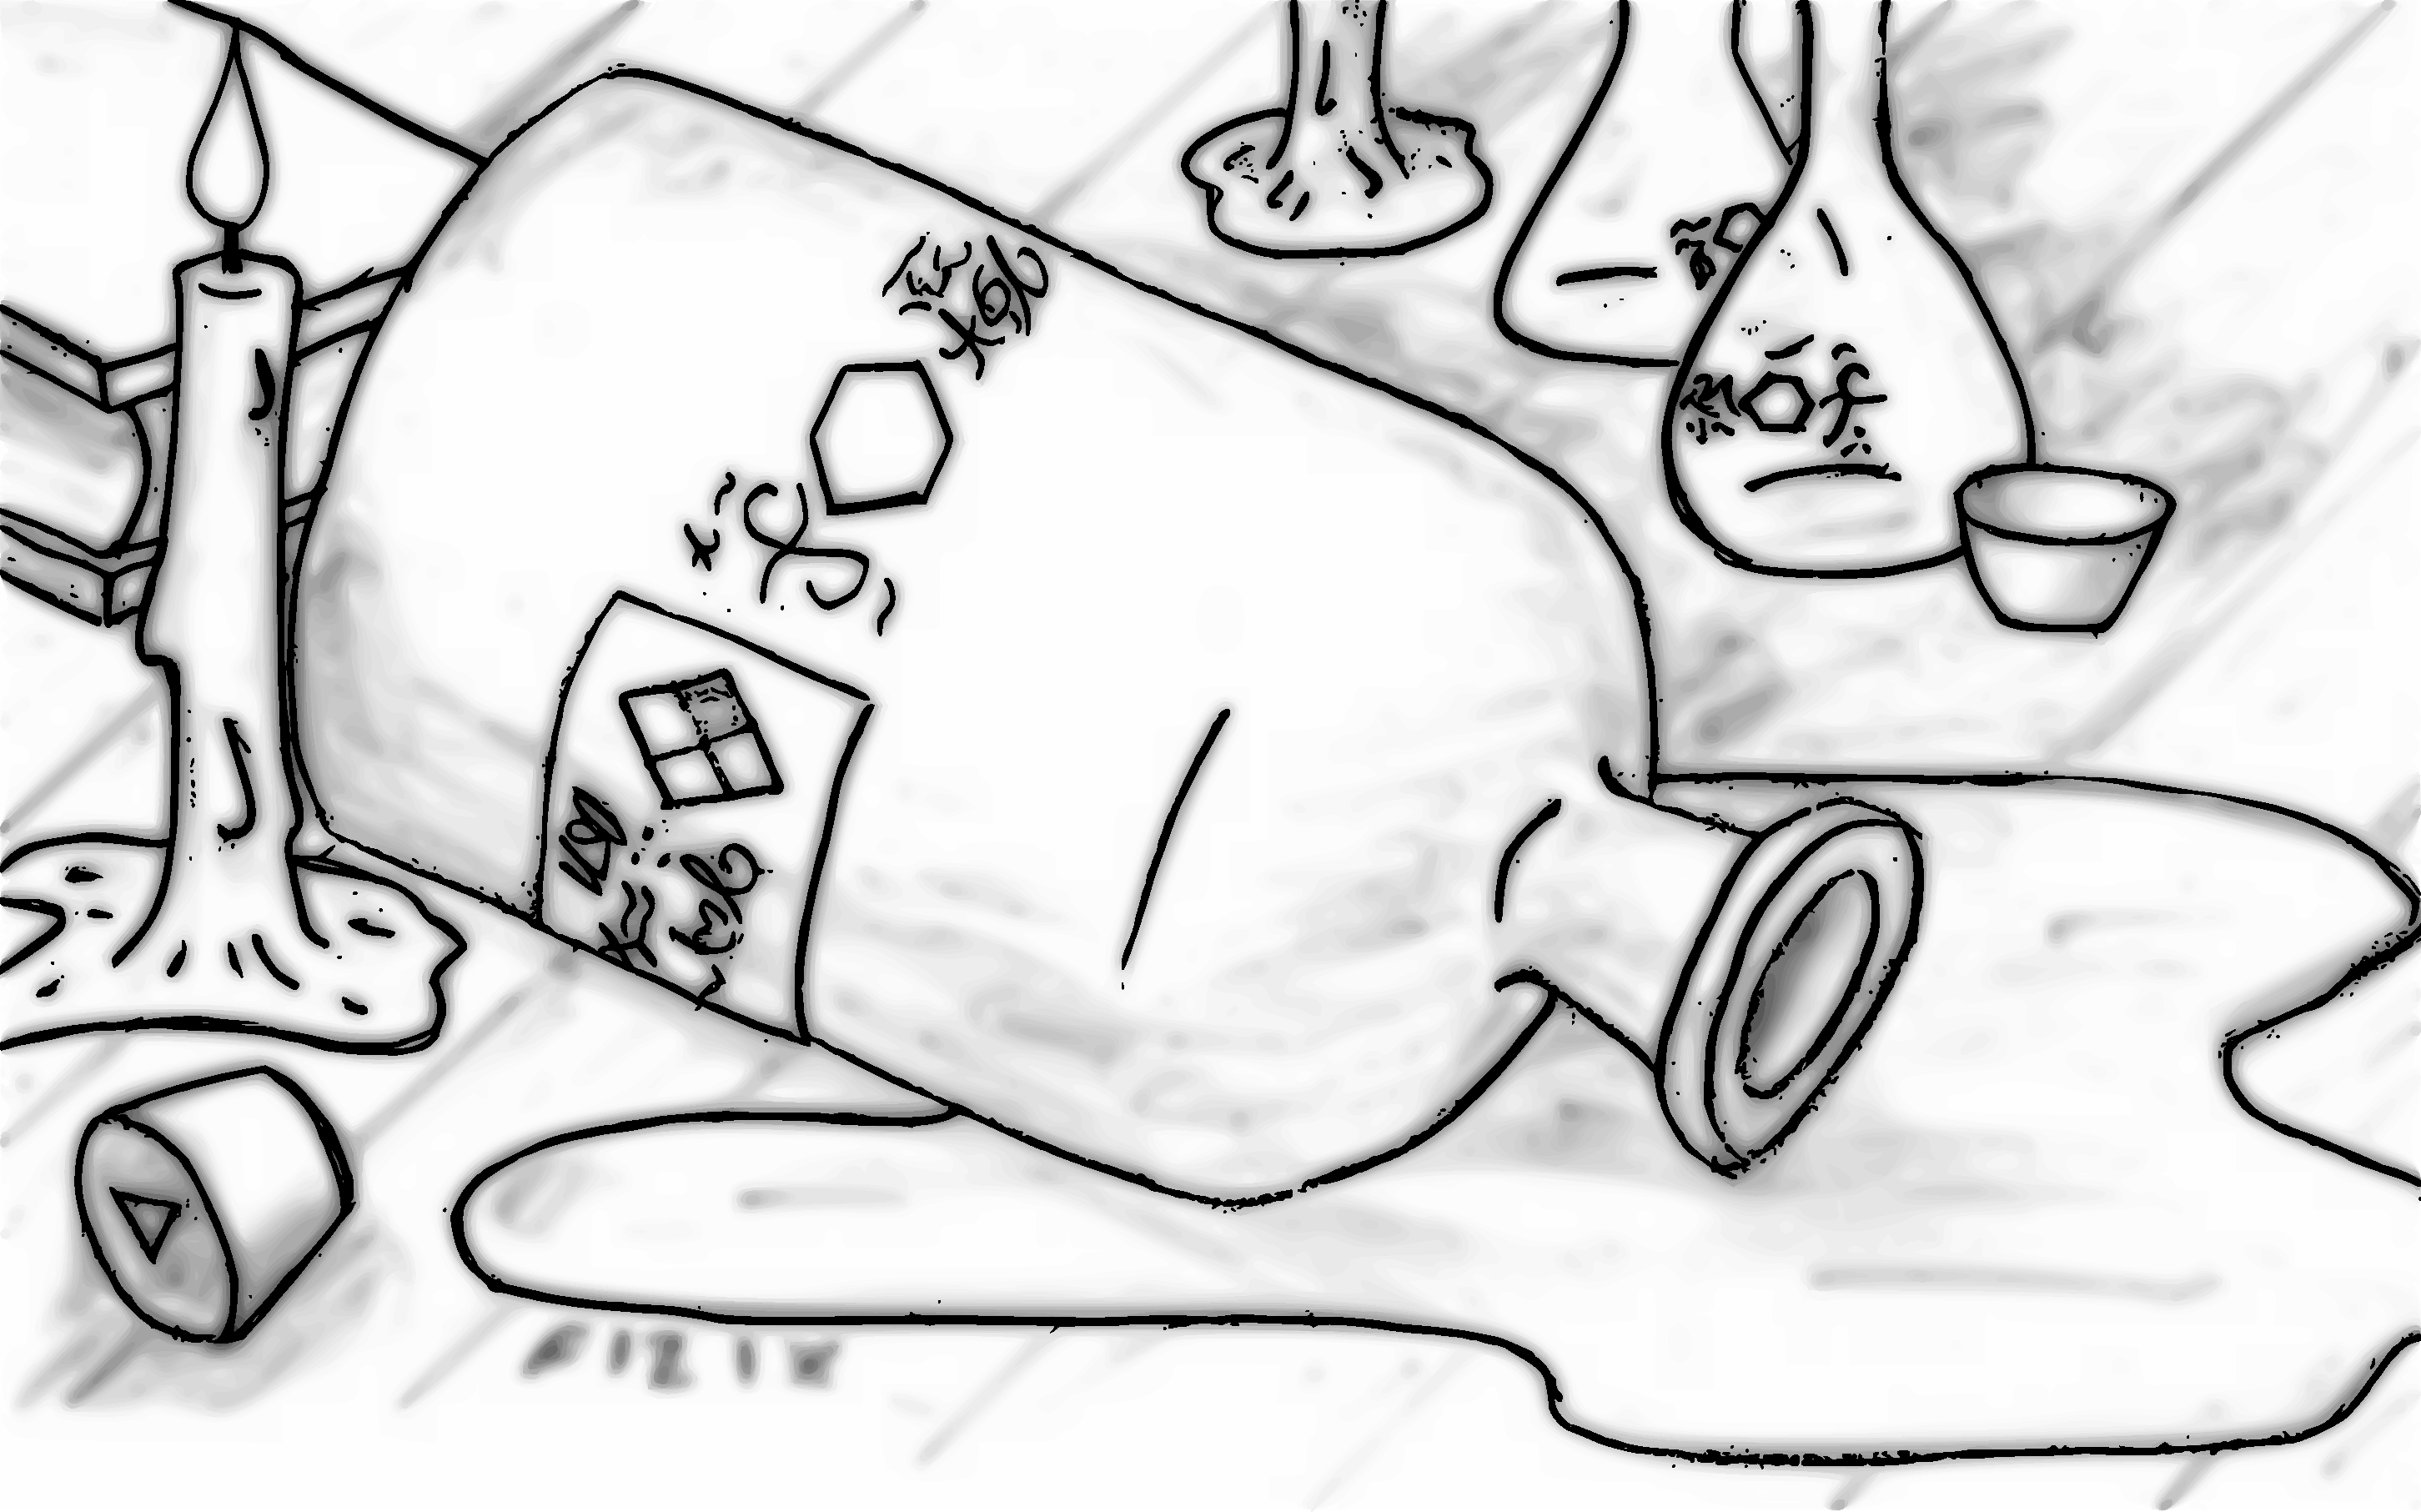
\includegraphics[width=\columnwidth]{alchemy.pdf}\label{alchemy}

\paragraph{Alchemy Jug:} This magical jug has the power to create a variety of mundane liquids upon the speaking of the proper command word.  One type of liquid can be created up to seven times each day.  The quantity of liquid created each time is dependent on the type of liquid.  The liquid can be poured from the jug at a maximum rate of two gallons per round.

\noindent \begin{tabular}{|p{.45\columnwidth}|p{.45\columnwidth}|}
\hline
Liquid	& Amount \\
\hline\hline
\rowcolor[gray]{0.9}Alcohol	& 1 gill (4 oz.) \\
Ammonia	& 1 quart \\
\rowcolor[gray]{0.9}Aqua regia	& 2 gills (8 oz.) \\
Beer	& 4 gallons \\
\rowcolor[gray]{0.9}Chlorine	& 8 drams (1 oz.) \\
Cyanide	& 4 drams ($^1$/$_2$ oz.) \\
\rowcolor[gray]{0.9}Oil	& 1 quart \\
Vinegar	& 2 gallons \\
\rowcolor[gray]{0.9}Water, fresh	& 8 gallons \\
Water, salt	& 16 gallons \\
\rowcolor[gray]{0.9}Wine	& 1 gallon \\
\hline
\end{tabular}

\end{multicols}

\noindent \begin{longtable}{|p{.05\textwidth}|p{.9\textwidth}|}
\multicolumn{2}{c}{Bag of Beans} \\
\hline
1d20	& Effect \\
\hline\hline
\endfirsthead
\multicolumn{2}{c}{\textit{\ldots continued from previous page}} \\
\hline
1d20	& Effect \\
\hline\hline
\endhead
\hline
\multicolumn{2}{r}{\textit{continued on next page \ldots}}\\
\endfoot
\hline
\endlastfoot
\rowcolor[gray]{0.9}1	& A chaotic evil treant springs from the ground and attacks creatures starting with the closest. \\
2	& A rope grows up to a height of 30 feet and leads to an inter-dimensional space as if a \textit{rope trick} spell had been cast.  The space remains for four hours, after which the rope becomes a \textit{rope of climbing}. \\
\rowcolor[gray]{0.9}3	& Flowers spring from the ground in a 120 yard radius.  During the following round, they emit a poisonous gas that causes any creatures that breathe it to fall asleep for 1d12 rounds (no save is allowed, creatures that don't sleep or breath are immune).  1d4~+~1 of those creatures who are put to sleep (chosen randomly by the GM) are granted a \textit{limited wish} based on their dreams.  The GM asks each affected player what their character dreamed about and grant a \textit{limited wish} based on that. \\
4	& When the bean is planted, the ground begins to rumble.  During the following round, a herd of mastodons appear and stampede toward the bean.  Their distance from the bean is determined by the environment (some locations would prohibit a sizable herd), but they always appear at the edge of the bean planter's vision.  The mastodons are otherwise normal animals and will either settle in the area, migrate elsewhere, or die off based on the environment. \\
\rowcolor[gray]{0.9}5	& A one-story tavern slowly rises from the ground, taking one round to fully assemble itself.  The tavern is fully furnished and occupied by \textit{unseen servants} who prepare a \textit{heroes' feast} on command.  The tavern remains for 3d4 days before vanishing.  If there isn't enough room for the tavern to grow, the bean is wasted. \\
6	& A burning bush grows from the ground with magic berries that act as \textit{fire seeds}.  1d4 acorn grenades and 2d4 holly berry bombs can be harvested from the bush. \\
\rowcolor[gray]{0.9}7	& A random creature emerges from the ground as if an \textit{iron flask} was opened.  The creature is angry and attacks any living creatures in sight.  If no creature is rolled on the first try, roll until one does; however, this creature is an illusory as if created by spectral force. \\
8	& A 20-foot tall tree springs from the ground.  24 apple-like fruits grow from the tree.  If the fruit is destroyed in any way, a random item from a \textit{robe of useful items} was used appears.  The tree and any remaining fruit vanishes after 48 hours, but any fruit that was picked and/or items that were created are permanent. \\
\rowcolor[gray]{0.9}9	& 1d4~+~3 eggs the same size as chicken eggs spring from the ground.  Any creature who eats an entire egg must save vs. poison.  If this save is successful, the creature gains one point to his intelligence score, otherwise it dies.  If an egg is split among multiple creatures or the yoke is separated from the white, it functions as a normal, nourishing egg. \\
10	& A massive beanstalk grows into the sky until it reaches a height of 5,000 feet.  The top of the beanstalk ends in the Elemental Plane of Air leading to a sky giant's castle.  If planted inside a normal, above-ground structure, the beanstalk destroys it.  If planted deep underground or in any other location where it can't break through the ceiling, the beanstalk dies. \\
\rowcolor[gray]{0.9}11	& A hostile earth elemental emerges from the ground and immediately switches minds with the bean's planter.  The hostile earth elemental attacks with any weapons the creature carries or wears but can't use any spells, and its intelligence remains the same.  If either or both of the bodies are destroyed, the effect is permanent and can't be reversed. \\
12	& An oak tree springs from the ground and produces 10d10 fruit made from a variety of precious materials such as ivory, jade, and amber.  Each ``fruit" is worth 10d10gp.  The tree is a mundane oak tree otherwise and doesn't radiate magic. \\
\rowcolor[gray]{0.9}13	& A \textit{big grasping hand} and a \textit{big clenched fist} rise from the ground as if the spells were cast.  They attack random creatures that are hostile to the planter of the bean within 90 feet and last 12 rounds. \\
14	& A young, adult red dragon emerges from the ground and begins to attack the closest creatures.  Its heart is a deep, red ruby the size of a human head, which acts as a fully charged \textit{wand of fireballs}. \\
\rowcolor[gray]{0.9}15	& Nothing seems to happen.  The weather changes randomly  in a 1d4 mile radius every 4d12 minutes as if \textit{control weather} had been cast.  The effect is permanent until \textit{dispel magic} is cast successfully at the site where the bean was planted. \\
16	& A map to a guarded treasure rises from the ground in the form of a finely embroidered tapestry.  The tapestry provides clues as to what challenges and treasure may be found. \\
\rowcolor[gray]{0.9}17	& A throne rises from the ground.  It can seat one human-shaped creature.  The throne has the power to transport that creature to any plane that they wish.  This power works 1d4 times before the throne disappears. \\
18	& The GM's choice of dinosaur emerges from the ground and behaves according to its nature. \\
\rowcolor[gray]{0.9}19	& Nothing seems to happen.  If the bean is dug up, it's discovered the bean has transformed into a 50 gp gem.  Further exploration reveals the entire area within a 5 mile radius has become a suitable site for gold mining. \\
20	& A huge, gaudy marble fountain with intricately crafted statues and frilly features rises from the ground.  The fountain contains 3d12 cp in its basin.  The fountain disappears after 12 rounds. \\
\end{longtable}

\begin{multicols}{2}

\paragraph{Bag of Beans:} This magical bag seems to belong to the same category of items as a \textit{wand of wonder}.  Only chaotically aligned creatures will truly prize a bag of this sort.  It is most often crafted in the form of a large sack of heavy cloth and usually contains 3d4 pebble-sized ``beans" when found.  The GM may determine that more or less beans are found.  Both the bag and the beans radiate magic if detect magic is cast.  In any case, only 1 or 2 of the beans contain beneficial powers.  Beneficial beans can create one or more useful items, bestow helpful effects upon the bag's owner, or contain other clearly beneficial powers.  The rest of the beans are bad beans, either summoning a random, angry, uncontrolled creature or casting an effective area spell.  It is highly unlikely that two bags will ever be found containing the same type of beans. 

To activate the power of a bean, it must be removed from the bag by hand, placed in dirt and watered.  In most cases, the power of the bean will manifest immediately with the creature or effect emerging from the ground where it was planted.  If a bean is removed by any other means, whether magical or mundane, or if one is taken out by hand and thrown, it immediately explodes inflicting 5d4 points of damage in a 10-foot radius around the one holding the bag.  If multiple beans are removed incorrectly at the same time (such as dumping the contents onto the ground), every bean removed explodes at once.  A successful save vs. spell reduces the damage by half.

When the last bean is planted (or explodes), the bag becomes a mundane sack.  All magical effects are cast at the 12\textsuperscript{th} level, unless otherwise specified.



\paragraph{Bag of Devouring:} This accursed bag is usually crafted in the form of an extra-large sack of heavy cloth.  It radiates magic if \textit{detect magic} is cast and will initially function as if it were a \textit{bag of holding} with a capacity of 250 lbs. or 30 cubic feet of material.  It is actually the visible mouthparts of a non-planar, extra-dimensional creature.  Turning the bag inside out dumps the current contents, closes the mouth and forces the bag to act as a mundane sack (though it still radiates magic). 

There's a 5\% cumulative chance each turn that items stored in the bag are eaten by the creature and expelled later into non-dimensional space causing them to be lost forever.  In addition, any time living flesh enters the bag (such as when someone puts their hand inside to retrieve an item), there's a 60\% chance that the creature attempts to eat him.  The base chance to avoid being eaten is 25\%, plus or minus 5\% for each point of the victim's strength---damage modifier score.  For example, a score of +2 would result in a 10\% bonus (or 35\% chance) not to get eaten.  A victim who fails this check is sucked completely into the bag, killed and eaten in one round, along with any other contents of the bag, to be expelled later.  Only a \textit{wish} spell or divine intervention may restore life to the victim.

If the GM wishes, the extra-dimensional creature can be hunted down and possibly even killed, but the GM must create statistics for the creature and determine the method necessary to reach the creature's non-planar home dimension.  If killed, the creature may contain a few random items (mostly mundane) from its most recent meal. 

\noindent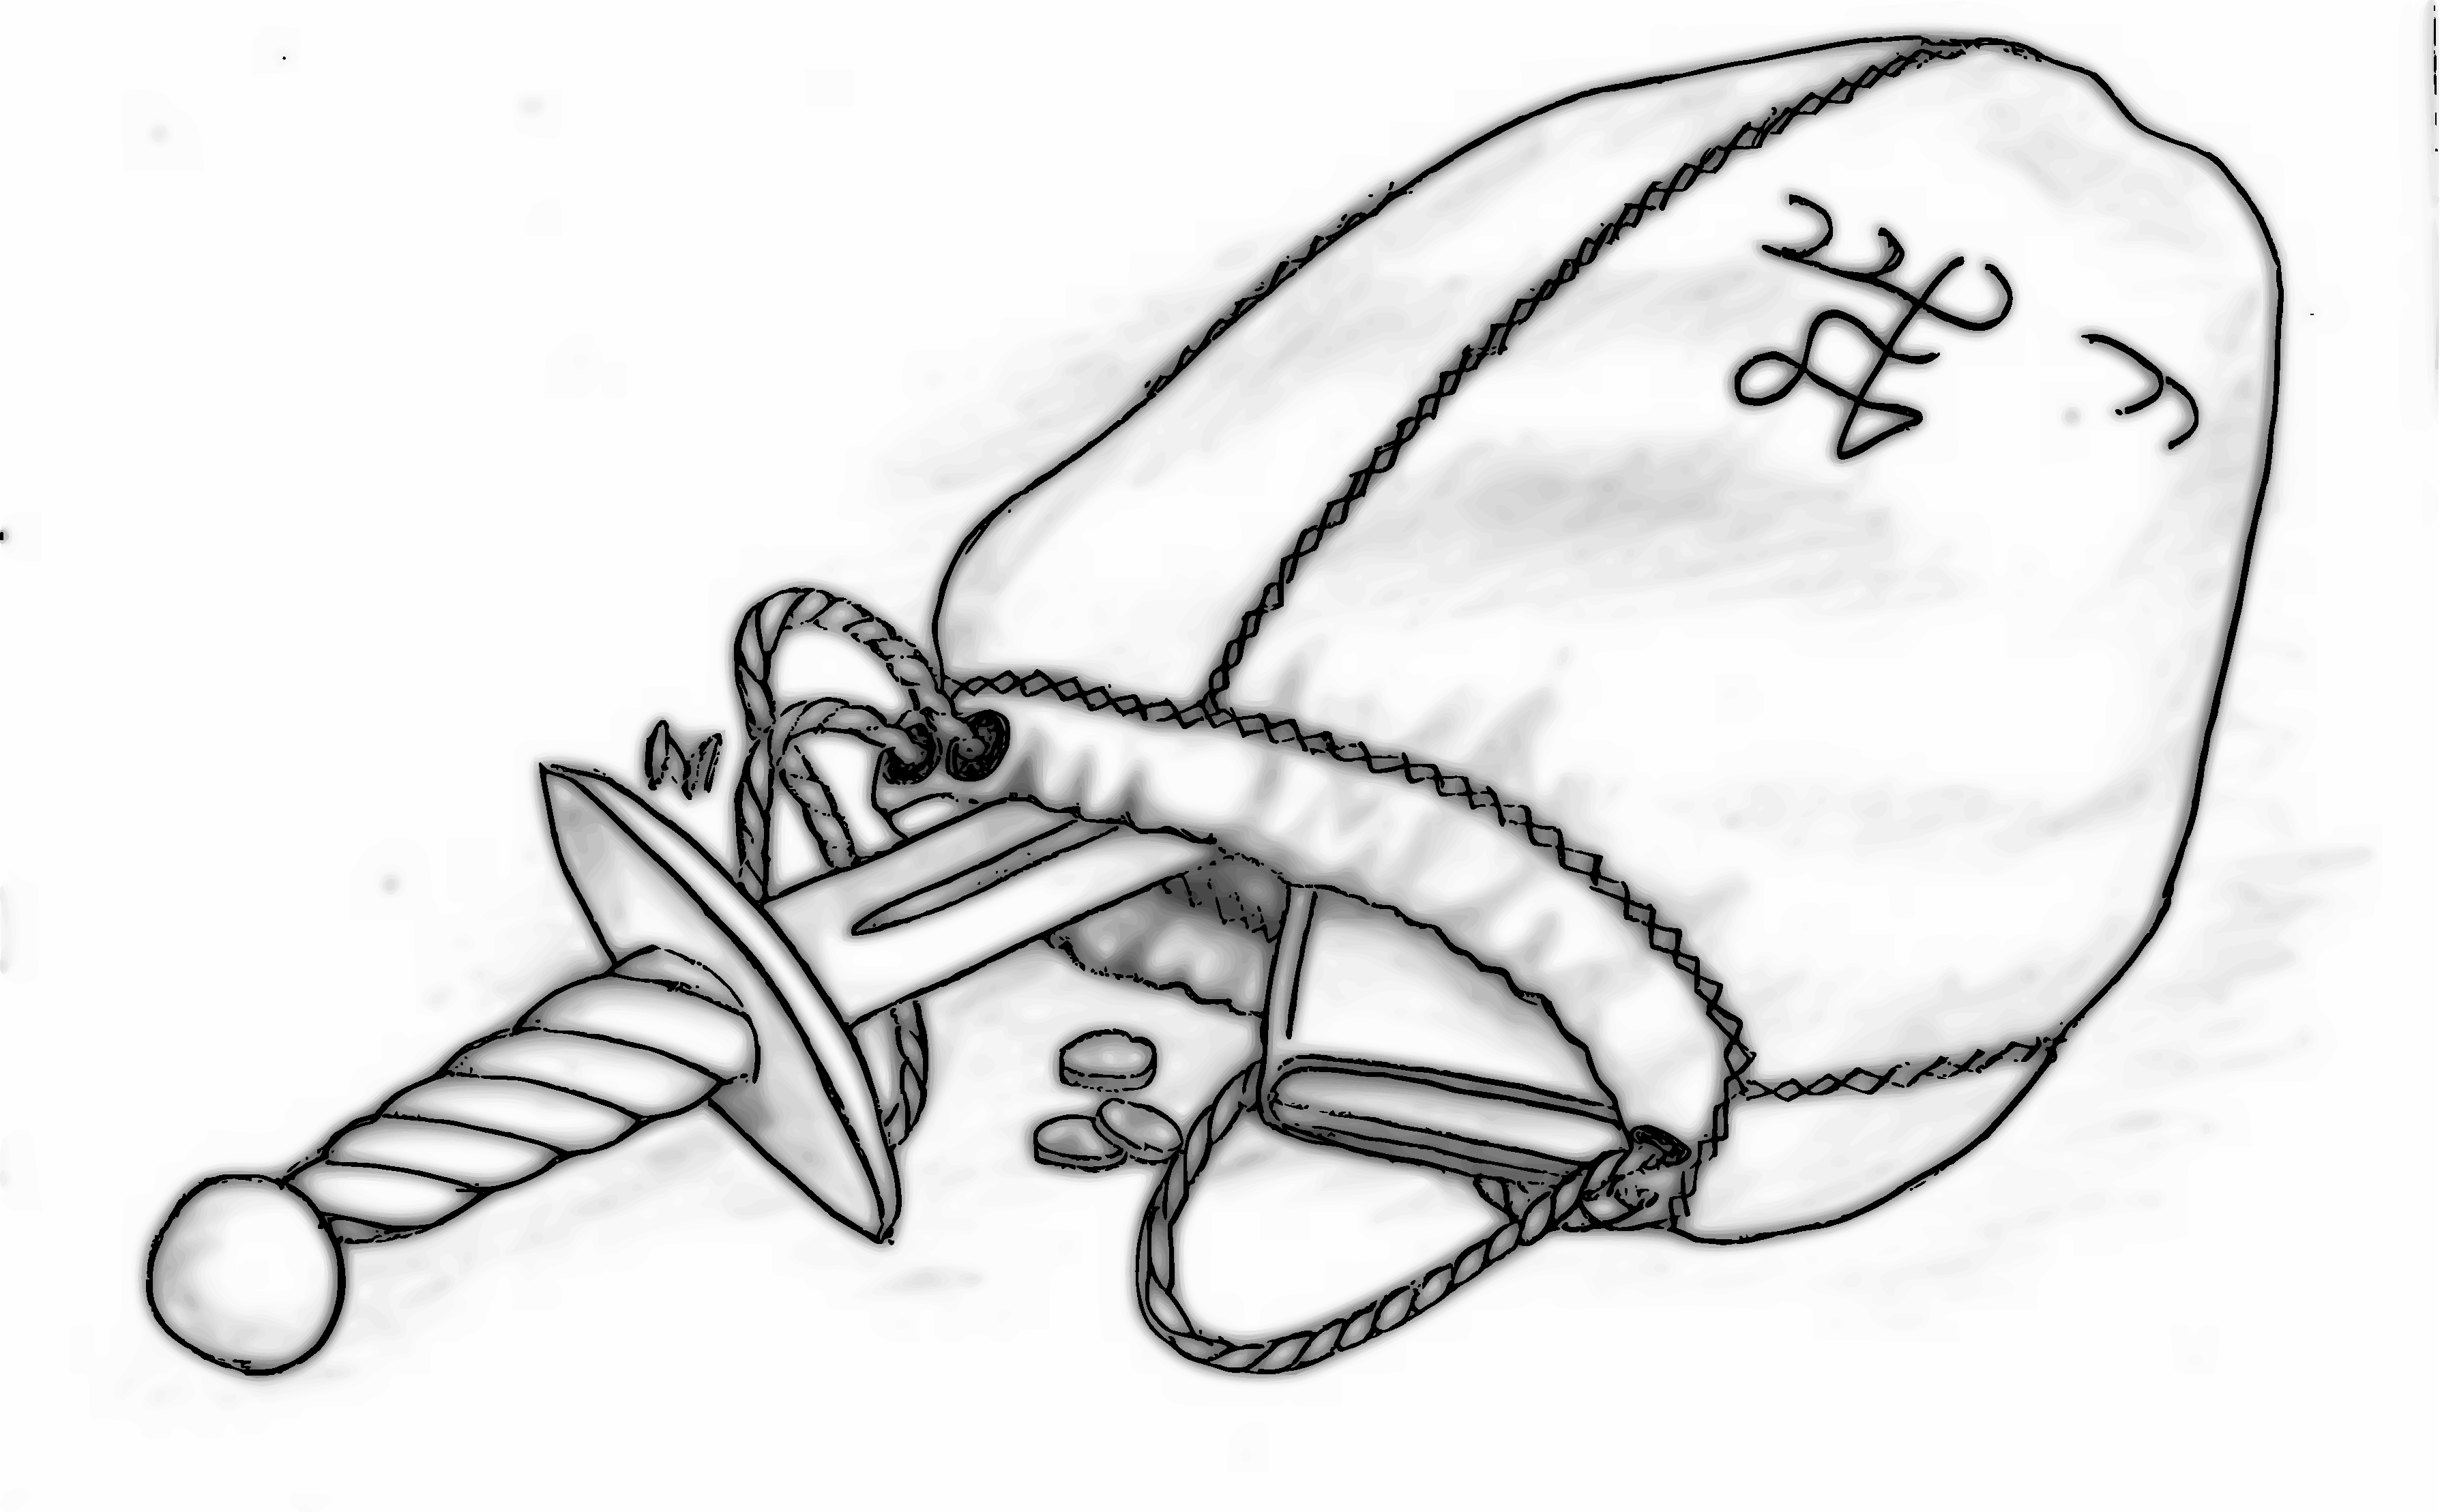
\includegraphics[width=\columnwidth]{bagofholding.pdf}\label{bagofholding}

\columnbreak

\paragraph{Bag of Holding:} This magical bag is crafted in the form of a mundane sack of heavy cloth, but radiates magic if \textit{detect magic} is cast.  The bag opens to a pocket dimension in Non-dimensional Space, and the inside is larger than the outside.  Turning the bag inside out dumps its contents and forces it to act as a mundane sack (though it still radiates magic).  The bag always weighs a fixed amount whether its non-planar space is full or empty.  There are several known varieties of this bag.  The size and weight of the bag, as well as its internal weight limit and volume depends on the type of bag found.  The GM may choose the type of bag or roll 1d100 and consult the following table.

\noindent \begin{tabular}{|p{.12\columnwidth}|p{.15\columnwidth}|p{.13\columnwidth}|p{.15\columnwidth}|p{.2\columnwidth}|}
\hline
1d100	& Common External Size*	& Bag's Weight	& Weight Limit	& Internal Volume \\
\hline\hline
\rowcolor[gray]{0.9}01--28	& Small or large		& 5 lbs.	& 50lbs.	& 10 cu. ft. \\
29--43	& Small or large		& 10 lbs.	& 100 lbs.	& 15 cu. ft. \\
\rowcolor[gray]{0.9}44--57	& Large or extra-large	& 10 lbs.	& 150 lbs.	& 20 cu. ft. \\
58--69	& Large or extra-large	& 15 lbs.	& 200 lbs.	& 25 cu. ft. \\
\rowcolor[gray]{0.9}70--79	& Extra-large			& 15 lbs.	& 250 lbs.	& 30 cu. ft. \\
80--87	& Extra-large			& 15 lbs.	& 500 lbs.	& 70 cu. ft. \\
\rowcolor[gray]{0.9}88--93	& Extra-large			& 35 lbs.	& 1,000 lbs.	& 150 cu. ft. \\
94--97	& Extra-large			& 60 lbs.	& 1,500 lbs.	& 250 cu. ft. \\
\rowcolor[gray]{0.9}98--00	& Extra-large			& 80 lbs.	& 2,000 lbs.	& 350 cu. ft. \\
\hline
\end{tabular}
\noindent\begin{tabular}{p{.95\columnwidth}}
*The GM may determine that an object cannot fit into the bag if it does not fit into the opening of a standard sack of the appropriate size. \\
\end{tabular}\vspace{.5em}

The bag begins to appear full externally as its internal volume begins to fill.  If the bag's weight limit or internal volume is exceeded or a sharp object pierces it (from inside or out), the bag is ruined and its contents are lost forever in non-dimensional space.  Placing a \textit{bag of holding} into a \textit{portable hole} sucks the \textit{bag of holding}, the \textit{portable hole}, and all their contents through an extra-dimensional rift into the Astral Plane, to be lost forever.  If a \textit{portable hole} is placed in a \textit{bag of holding} it sucks the \textit{bag of holding}, the \textit{portable hole}, all their contents, plus everything in a 10-foot radius through an extra-dimensional rift into the Astral Plane, to be lost forever.

\paragraph{Bag of Transmuting:} This accursed bag is crafted in the form of a mundane sack of heavy cloth, but radiates magic if \textit{detect magic} is cast.  The bag initially functions as if it were a \textit{bag of holding} of any random type, but after 1d4~+~1 days all precious metal and gemstones within the bag are changed into common metal and worthless rocks.  Magical items (other than artifacts and relics) become permanently mundane and worthless without the benefit of a save.  Turning the bag inside out dumps its contents and forces it to act as a mundane sack (though it still radiates magic).

\paragraph{Bag of Tricks:} This magical bag is most often crafted in the form of a mundane tiny sack, but radiates magic if \textit{detect magic} is cast.  When the bag is otherwise empty, anyone reaching inside of it feels a small, fuzzy ball.  When the ball is removed from the bag and thrown up to 20' away, a randomly generated animal is created.  Only one animal can be created at a time.  The animal understands, obeys and fights to the best of its ability for the one who created it.  The creator can order it back into the bag at any time, or it will remain in existence for one turn or until slain.  Up to 10 animals can be created per week.  Turning the bag inside out causes the furry ball to vanish and forces the bag to act as a mundane sack (though it still radiates magic).  

There are three known varieties of these bags, each of which produces a different collection of animals.  To determine the bag found, roll 1d10.  On a 1--5 the bag is type A, on 6--8 the bag is type B, and on 9--10 the bag is type C.

\end{multicols}

\noindent \begin{tabular}{|p{.05\textwidth}|p{.15\textwidth}|p{.05\textwidth}|p{.05\textwidth}|p{.05\textwidth}|p{.5\textwidth}|}
\multicolumn{6}{c}{Bag of Tricks} \\
\multicolumn{6}{c}{Type A (1-5)} \\
\hline
1d8	& Animal	& AC	& HD	& HP	& Attack (Damage) \\
\hline\hline
\rowcolor[gray]{0.9}1	& Weasel		& 6		& $^1$/$_2$	& 2		& Bite (1) \\
2	& Skunk		& 9		& $^1$/$_2$	& 2		& Musk \\
\rowcolor[gray]{0.9}3	& Badger		& 4		& 1~+~2		& 7		& 2 claws (1d2)~+~bite (1d3) \\
4	& Wolf		& 7		& 2~+~2		& 12	& Bite (1d4~+~1) \\
\rowcolor[gray]{0.9}5	& Lynx, giant	& 6		& 2~+~2		& 12	& 2 claws (1d3)~+~2 rear claws (1d2)~+~bite (1d4) \\
7	& Boar		& 7		& 3~+~3		& 18	& Tusks (1d10~+~2) \\
\rowcolor[gray]{0.9}8	& Stag, giant	& 7		& 5			& 25	& Headbutt (4d4) or 2 hooves (1d4) \\
\hline
\end{tabular}

\noindent \begin{tabular}{|p{.05\textwidth}|p{.15\textwidth}|p{.05\textwidth}|p{.05\textwidth}|p{.05\textwidth}|p{.5\textwidth}|}
\multicolumn{6}{c}{Type B (6-8)} \\
\hline
1d8	& Animal	& AC	& HD	& HP	& Attack (Damage) \\
\hline\hline
\rowcolor[gray]{0.9}1	& Rat		& 7& 	$^1$/$_2$	& 2	& Bite (1) \\
2	& Owl		& 7	& $^1$/$_2$	& 3	& 2 talons (1d3) \\
\rowcolor[gray]{0.9}3	& Dog		& 7	& 1~+~1		& 6	& Bite (1d6) \\
4	& Goat		& 7	& 1~+~1		& 8	& Headbutt (1d6) \\
\rowcolor[gray]{0.9}5	& Ram		& 6	& 2			& 10	& Headbutt (1d4~+~1) \\
6	& Bull		& 7	& 4			& 20	& 2 horns (1d6) \\
\rowcolor[gray]{0.9}7	& Brown Bear	& 6	& 5~+~5	& 30	& 2 claws (1d6)~+~hug (2d6) or bite (1d8) \\
8	& Lion		& 5	& 5~+~2		& 28	& 2 claws (1d4)~+~rear claws (1d6~+~1) or bite (1d10) \\
\hline
\end{tabular}

\noindent \begin{tabular}{|p{.05\textwidth}|p{.15\textwidth}|p{.05\textwidth}|p{.05\textwidth}|p{.05\textwidth}|p{.5\textwidth}|}
\multicolumn{6}{c}{Type C (9-10)} \\
\hline
1d8	& Animal	& AC	& HD	& HP	& Attack (Damage) \\
\hline\hline
\rowcolor[gray]{0.9}1	& Jackal	& 7	& $^1$/$_2$	& 2	& Bite (1d2) \\
2	& Eagle		& 7	& 1		& 5	& 2 talons (1d2) \\
\rowcolor[gray]{0.9}3	& Baboon	& 7	& 1~+~1	& 6	& Bite (1d4) \\
4	& Ostrich	& 7	& 3		& 15	& Kick (1d8) \\
\rowcolor[gray]{0.9}5	& Leopard	& 6	& 3~+~2	& 17	& 2 claws (1d3)~+~2 rear claws (1d4) or bite (1d6) \\
6	& Jaguar	& 6	& 4~+~2	& 21	& 2 claws (1d3)~+~2 rear claws (1d4~+~1) or bite (1d8) \\
\rowcolor[gray]{0.9}7	& Buffalo	& 7	& 5		& 25	& 2 horns (1d8) \\
8	& Tiger		& 6	& 5~+~5	& 30	& 2 claws (1d4~+~1)~+~2 rear claws (2d4) or bite (1d10) \\
\hline
\end{tabular}

\begin{multicols}{2}

\paragraph{Beaker of Plentiful Potions:} This magical beaker is crafted in the form of a mundane piece of alchemist's laboratory equipment and sealed with an ordinary cork.  However, it radiates magic if \textit{detect magic} is cast and has the power to create up to 1d4~+~1 randomly determined potions and/or oils.  Any type of potion or oil is possible, including poisoned and other accursed potions, and the same type may be determined twice.  The beaker creates 1d4~+~1 doses of each type of potion generated.  Record the names of the potions and the number of doses per potion in the order that they are generated, as they will be poured from the beaker one dose per round in that order. 

If the beaker creates only two types of potions, it can dispense all of the doses of both potions up to three times per week but no more than once per day.  If three types of potions are created, it can dispense all of the doses up to twice per week but no more than once each per day.  If four or five potions are created, it can dispense all of the doses once per week.  

The beaker gradually loses its magic after its sealed stopper is first removed.  Each month thereafter, it permanently loses the power to create one randomly determined potion.  

\paragraph{Decanter of Endless Water:} This magical decanter is crafted in the form of an inexpensive vessel to serve water and sealed with an ordinary cork.  It radiates an aura of magic if \textit{detect magic} is cast.  When the stopper is removed and a specific magic command is spoken, the decanter exhibits one of the following powers in either fresh or salt water.  Another specific command word must be spoken to make the power stop.

\underline{Stream:} When this power is activated, the decanter pours forth 1 gallon per round.

\underline{Fountain:} When this power is activated, the decanter projects a light stream 5 foot long, pouring forth 5 gallons per round.

\underline{Geyser:} When this power is activated, the decanter sprays a heavy stream 20 foot long, pouring forth 30 gallons per round.  The geyser creates backpressure.  If the user is not braced, balanced or otherwise prepared for the force of the water, the user is knocked back and the GM may require that he must roll a successful wisdom check to continue to hold on to the decanter.  A dropped decanter with its geyser power activated skitters across the ground at a speed of 15 to 18, depending on the surface.

Man-sized or smaller creatures caught in the path of the geyser must roll a strength check each round or be knocked prone, while tiny-sized or smaller vermin (insects and animals) are killed instantly.

It may be possible to use the geyser power of the decanter as a method of propulsion under the right conditions.  Underwater, in frictionless or zero gravity settings, a man-sized user would be pushed at a speed of 6, huge and gargantuan users at a speed of 3, small users at a speed of 9 and tiny users at a speed of 12.  Underwater or in other 3 dimensional spaces, the user may be treated as a flier an SC1 and MC4.  The constant flow of water can also be used by clever engineers to power small water powered devices.

\paragraph{Efreeti Bottle:} This magical bottle is most often crafted from bronze or brass, with a lead stopper sealed with strange arcane symbols.  A small wisp of smoke may be seen to escape the bottle from time to time, and the bottle radiates magic if \textit{detect magic} is cast.  When the sealed stopper is removed, an efreeti is immediately released.  10\% of the time, the efreeti is hostile and attacks the user.  Another 10\% of the time, the efreeti grants the user three \textit{wishes} before returning to his home plane.  The remaining 80\% of the time, the efreeti serves the user for 1,001 days before returning to its home plane.

\noindent
\includegraphics[width=3.6in, height=1in]{testblock.pdf}

\paragraph{Everfull Purse:} This magical purse is most often crafted in the form of a mundane, tiny sack or small belt pouch, but radiates magic if \textit{detect magic} is cast.  When found, it will always contain a number of coins of various metal and possibly a few small gemstones.  The purse becomes permanently mundane if left empty or inside out for more than 1d4 rounds, however, if at least one coin or gemstone of an appropriate type is left inside, the purse will create 25 more of that type of coin (and/or 25 more gemstones) each day.  There are 3 known varieties of this purse.  The GM should roll 1d100 to determine which type is found.  The type of purse determines the types of coins or gemstones it can create each day.  This table can also indicate the number and types of coins and/or gemstones found inside the purse, but that number can be different depending upon its use by its previous owner.  It can contain coins and gemstones that it is unable to create without affecting its power.

\noindent \begin{tabular}{|p{.12\columnwidth}|p{.08\columnwidth}|p{.08\columnwidth}|p{.08\columnwidth}|p{.08\columnwidth}|p{.08\columnwidth}|p{.13\columnwidth}|}
\hline
1d100	& CP	& SP	& EP	& GP	& PP	& Gems* \\
\hline\hline
\rowcolor[gray]{0.9}01--50	& --	& 26	& 26	& 26	& --	& -- \\
51--90	& 26	& --	& 26	& --	& 26	& -- \\
\rowcolor[gray]{0.9}91--00	& 26	& --	& 26	& --	& --	& 26 \\
\hline
\end{tabular}
\noindent\begin{tabular}{p{.95\columnwidth}}
*Ornamental, semi-precious or fancy gemstones, up to 100gp maximum value each \\
\end{tabular}\vspace{.5em}

\paragraph{Eversmoking Bottle:} This magical bottle is most often crafted in the form and appearance of an \textit{efreeti bottle}, but when the sealed stopper is removed, thick, opaque smoke billows out.  The smoke instantly fills 50,000 cubic feet in one round and 10,000 cubic feet each additional round, until 120,000 cubic feet of smoke feet pour out or a command word is spoken and the jug is resealed.  The smoke dissipates only after the bottle is resealed, regardless of wind or weather.

\paragraph{Flask of Curses:} Though commonly called a flask, this accursed item is just as often crafted in the form of any other beneficial magical bottle, beaker, decanter, or jug.  It radiates magic but does not reveal its curse if \textit{detect magic} is cast.  Opening its sealed stopper inflicts a curse upon the user and his associates.  The GM must determine the nature of the curse.  It may simply cast the reverse of a \textit{bless} spell upon the user and his allies, it could release a powerful creature that immediately attacks the user and his allies, or the GM may determine the nature of the curse by referring to the suggestions given for a \textit{cursed scroll}.  Each flask holds only a single curse.  Once its curse is released, the flask becomes a mundane object of the appropriate type.

\paragraph{Handy Haversack:} This magical haversack is crafted in the form of a well-used yet well-made backpack of finely tanned leather with brass rings and buckles.  It is made with one larger central pouch and two smaller side pouches.  Each pouch opens to a pocket dimension in Non-dimensional Space, and the inside of each is larger than the outside.  The central pouch (which would normally hold only 30 pounds of gear) holds up to 80 pounds within eight cubic feet.  The two side pouches (which would normally hold only 10 pounds each) hold up to 20 pounds within two cubic feet each.  Whenever the wearer reaches into the correct pouch and speaks the name of a desired item, that item (assuming the item is within that pouch) shuffles to the top of the other items.  The haversack and all items inside gain a  +2 bonus on all saving throws, however in all other ways it acts as a \textit{bag of holding}.

\paragraph{Iron Flask:} These magical flasks are crafted of wrought iron, usually inlaid with silver runes, with a brass stopper sealed with strange arcane symbols.  The power of the flask allows its user to attempt to trap any extra-planar creature and enforce the creature's servitude.  When initially found, the GM should roll 1d100 to determine whether the flask is empty or already holds an extra-planar creature.
 
\noindent \begin{tabular}{|p{.3\columnwidth}|p{.6\columnwidth}|}
\hline
1d100	& Contents \\
\hline\hline
\rowcolor[gray]{0.9}01--50	& Empty \\
51--54	& Air elemental \\
\rowcolor[gray]{0.9}55--65	& Djinni \\
66--69	& Earth elemental \\
\rowcolor[gray]{0.9}70--72	& Efreeti \\
73--76	& Fire elemental \\
\rowcolor[gray]{0.9}77--86	& Invisible stalker \\
87--89	& Rakshasa \\
\rowcolor[gray]{0.9}90--93	& Salamander \\
94--97	& Water elemental \\
\rowcolor[gray]{0.9}98--99	& Wind walker \\
00	& Xorn \\
\hline
\end{tabular}

If the flask is empty, one extra-planar creature of the user's choice within 60 feet may be trapped inside the flask, unless its magic resistance overcomes the effect (as applicable) or it makes a successful save vs. spell when the flask is unsealed and a command word spoken.  

If the user speaks the command word while freeing a trapped creature, the creature can be forced to serve the user of the flask for one turn or perform a minor service requiring no more than one hour.  If the user of the flask frees a creature without speaking the command word, the GM should roll to determine the creature's reaction to the user.  

If the user attempts to trap the same creature in the flask more than once, it gains a cumulative +2 bonus to its saving throw and immediately becomes very angry and hostile toward the user.

\paragraph{Portable Hole:} This magical circle of cloth is crafted from the webs of a phase spider interwoven with strands of the Ethereal Plane and beams of light from the Astral Plane.  It can be folded up to be as small as a handkerchief, but when opened fully the cloth is 6 feet in diameter.  When spread upon any surface, it opens into a non-planar space, 10 feet deep, within Non-dimensional Space.  This hole can be closed from inside or out by simply taking hold of the edges of the cloth and folding it up.  Either way, the entrance disappears, but anything inside the hole remains in the non-planar space. 

The only air in the non-planar space is that which enters when it is opened.  The non-planar space contains enough air to supply one man-sized or two small-sized creatures for 1 turn.  The cloth does not accumulate weight even if its non-planar space is filled.  Each portable hole opens on its own particular non-planar space.  

Placing a \textit{bag of holding} into a \textit{portable hole} sucks the \textit{bag of holding}, the \textit{portable hole}, and all their contents through an extra-dimensional rift into the Astral Plane, to be lost forever.  If a \textit{portable hole} is placed in a \textit{bag of holding} it sucks the \textit{bag of holding}, the \textit{portable hole}, all their contents, plus everything in a 10-foot radius through an extra-dimensional rift into the Astral Plane, to be lost forever.

\paragraph{Pouch of Accessibility:} This magical pouch is crafted in the form of a mundane large belt pouch, but contains 30 pockets inside it.  Each pocket opens to a non-planar space within Non-dimensional Space capable of holding up to 10 pounds or one cubic foot of volume.  The pouch weighs 1 pound when empty and 4 pounds when its non-planar spaces are filled.  The user can summon an item to the top of the pouch by reaching in and speaking the item's name.  In all other ways the pouch acts as a \textit{bag of holding}.

\subsection{CANDLES, DUSTS \& STONES}

\index{Wondrous Items!Candles, Dusts, \& Stones}Mundane candles serve as light sources while reading or for lighting the way while walking through darkened halls.  Candles are also commonly used in religious services for illumination while reading the sacred texts, symbolic adornment or to aid in prayer and meditation.  Two types of candles are listed on the standard equipment tables, inexpensive tallow candles and the more expensive wax candles.  Tallow candles consist of animal fats and are often used by commoners.  Mundane wax candles are usually made from beeswax (either from normal or giant-sized bees), but magical candles can be made from more exotic sources, such as spermaceti, or bayberry.  Only candles that have been specially made from the purest grade of the correct wax by an expert candle maker and enhanced with the proper incense, perfume, oil, or herbs can be used to craft magical candles.  Wicks for mundane candles are typically made of thin strips of cloth or cord, while those for magical candles are made of woven silk.

Mundane dusts and powders that may be known to the player characters include such things as talc, flour, pepper, various salts, metallic flakes, powdered herbs, sand or even normal dirt.  If the GM allows, some combinations of otherwise mundane dusts and powders may have alchemical or medicinal effects (refer to ointment).  Mundane dusts and powders are similar in use, but dust is less absorbent and usually has lighter and smaller particles than powder giving dust a larger dispersion area.  If in doubt whether a mundane substance is a dust or a powder, the GM has the final say.  

Dusts and powders can be kept in any small box or bowl with a hinged lid (refer to ointment).  When kept in this manner, they may be poured directly onto a willing target or thrown at an opponent.  A handful of dust may be thrown to form a cloud with a 10-foot radius up to 10 feet away, and a handful of powder may be thrown to affect a single individual up to 5 feet away.  Oftentimes, however, they are found in tiny pouches made of cloth or paper.  The dust or powder can be shaken out of the pouch to cover the surrounding area.  Dust spreads into a cloud with a 10-foot radius around the user, and powder spreads into a cloud with a 5-foot radius.  When dusts and powders are spread in this manner, they can easily affect the user, either intentionally or accidentally.  Resourceful characters will sometimes repackage dusts and powders into hollow, stoppered blow tubes, 2 to 6 inches long, made of glass, metal, bone, wood or similar materials.  When the stoppers are removed and the blow tube is blown into, it causes the dust to form into a cone-shaped cloud 20 feet long and 10 feet wide at its widest point.  Powder blown through a blow tube forms a cone-shaped cloud 10 feet long and 5 feet wide.  When blown through a tube, dusts and powders have no chance to affect the user unless he immediately enters the cloud or some other condition such as the wind or limited space causes him to be covered by it.  A cloud of dust or powder (regardless of the dispersion method) lasts only for the remainder of the round.  Magical dusts and powders may follow similar guidelines given above, or they may be so powerful or have specific effects that special procedures must be followed.  The particular methods of dispersion for each are described in their descriptions.

Mundane glues are various substances, usually in liquid or paste form, that cause objects to stick together.  Thinner objects are generally easier to glue together than thicker objects, but the material of the objects must also be considered.  Once the substance is placed between the objects to be glued together, it must harden either by evaporation or by alchemical reaction.  Mundane glue is used when making compound bows, crossbows, arrows, spears and similar weapons.  It is made from a wide variety of natural substances such as birch-bark-tar, spruce-gum and animal fat, animal bones and teeth, egg whites, etc.  Mundane solvents are various substances that dissolve or break down other substances.  Common mundane solvents include various types of alcohol, turpentine and vinegar.  Magical glues and solvents are crafted to exaggerate these substance's natural properties.

Mundane incense is a combination of powdered herbs and chopped flower petals that are formed into small, rectangular cubes.  The cube of incense is then mixed with alcohol and burned or mixed with water and boiled in a small censer to give off a scent.  Magical incense releases its power (and its scent) as it is burned or boiled.

\textit{Ioun stones} are a special type of magical stone.  Their description and use are fully described below.  The GM is advised that these magical stones are generally rare, unusual and harder to find than the magic item tables would imply.

Ointments, whether mundane or magical, are usually found in jars or small boxes made of wood, metal, ivory, ceramic, glass, crystal or similar materials, complete with lids and cotton applicators.  Mundane ointments are creamy herbal remedies or medicinal salves and unguents.  Touted to stop hair loss and snoring or to cure pink eye and other common ailments, they are of little use or value to the average group of player characters.  It is up to the GM as to the effectiveness of any mundane ointments; however, many creatures prize magical ointment.

Pigments are a form of paint made from colorful powders mixed with a fluid such as water or oil.  They are stored in small pots made from glass, ceramic or similar material and sealed with a cork.

Magical stones are crafted from or appear to be common pieces of rock.  

\noindent \begin{minipage}{\columnwidth}
\captionof{table}{Candles, Dusts, and Stones}
\noindent \begin{tabular}{|p{.12\columnwidth}|p{.5\columnwidth}|p{.23\columnwidth}|}
\hline
1d20	& Item	& XP \\
\hline\hline
\rowcolor[gray]{0.9}1	& Candle of Invocation (Priest)	& 1,000/candle \\
2	& Dust of Appearance	& 1,000 \\
\rowcolor[gray]{0.9}3	& Dust of Disappearance	& 2,000 \\
4	& Dust of Dryness	& 1,000 \\
\rowcolor[gray]{0.9}5	& Dust of Illusion	& 1,000 \\
6	& Dust of Sneezing and Choking	& Accursed \\
\rowcolor[gray]{0.9}7	& Dust of Tracelessness	& 500 \\
8	& Incense of Meditation (Priest)	& 500 \\
\rowcolor[gray]{0.9}9	& Incense of Obsession (Priest)	& Accursed \\
10	& Ioun Stones	& 300/stone \\
\rowcolor[gray]{0.9}11	& Marvelous Pigments	& 500/pot \\
12	& Miracle Ointment	& 500 \\
\rowcolor[gray]{0.9}13	& Philosopher's Stone (Wizard)	& 1,000 \\
14	& Smoke Powder	& -- \\
\rowcolor[gray]{0.9}15	& Sovereign Glue	& 1,000 \\
16	& Stone of Controlling Earth Elementals	& 1,500 \\
\rowcolor[gray]{0.9}17	& Stone of Good Luck (Luckstone)	& 3,000 \\
18	& Stone of Weight (Loadstone)	& Accursed \\
\rowcolor[gray]{0.9}19	& Universal Solvent	& 1,000 \\
20	& GM's Choice	& -- \\
\hline
\end{tabular}

\end{minipage}

\paragraph{Candle of Invocation:} These magical candles are crafted in the form of mundane, tapered wax candles of the sort appropriate for use during the religious ceremonies of any one of the 9 alignments.  Usually found singly, but sometimes found in matched pairs, these candles are between 8 to 12 inches long and between $^1$/$_2$ to 1 inch thick.  The candles radiate magic if \textit{detect magic} is cast and radiate the alignment of the priest who crafted them if \textit{detect good or evil} or similar is cast.

If any priest (including a druid) of the same alignment lights a candle, he immediately gains 2 levels (if multi or dual classed only priest levels are affected).  He gains all of the benefits of being higher level including better chances to turn or dominate the undead and to cast additional spells of levels previously before unknown.  The first time a candle is lit on a particular day, the GM should allow the player a few minutes of real time to choose the additional spells granted by its power.  The priest retains these benefits for as long as the candle burns somewhere within a 25-foot radius of the priest (the candle can be placed in a shelter, such as a lantern, to protect the flame).  Each candle burns for up to four hours, but can be extinguished by any normal means for later use.  The GM must keep precise track of every round (or minute) that the candle burns.  The bonus levels can be gained multiple times per day, but the bonus spells are only gained once. 

While the candle is burning a priest can use its power to create an extra-dimensional \textit{gate}, but doing so completely consumes the remainder of the candle.  The extra-dimensional creature that responds to the \textit{gate} will be of the candle's alignment.  Otherwise, the GM has a few options as to how to handle the specifics of this power.  He may base the chance of successfully creating the \textit{gate} upon the percentage of candle that remains when the \textit{gate} power is activated.  For example, a previously unburned candle has a 100\% chance of successfully creating the \textit{gate} while a candle that has previously burned for 3 hours has only a 25\% chance of success.  Optionally, the GM may always allow the \textit{gate} power to function but determine the strength of the creature attracted to it based upon the amount of candle remaining, so that a full candle will attract a very powerful extra-planar being while a stub of a candle will attract only weaker varieties.  In either case, the GM may also determine that the extra-planar creature only remains for the amount of time that was left on the candle when the \textit{gate} was created, up to 4 hours maximum.

If a character other than a priest lights a candle matching his alignment, it generates a favorable aura for that particular character.  The GM must determine the nature of the favorable aura on a case-by-case basis, but the power usually manifests as minor divine intervention in the form of a +1 bonus to all saving throws, to hit or on damage rolls when battling an enemy with diametrically opposed alignment.

If a character lights a candle of a different alignment than his own, the candle may inflict an unfavorable aura upon him for a minimum of 1 turn.  The GM should determine the negative effects based upon how different the alignments are with the most severe penalties inflicted upon priests of a diametrically opposed alignment.

\paragraph{Dust of Appearance:} This magical dust seems mundane but radiates magic if \textit{detect magic} is cast.  Upon close inspection, the dust is revealed to be very fine, very light and to have a metallic quality.  It is commonly found in silk pouches or bone blow tubes.  A pouch can be shaken out to cover a 10-foot radius area around on the user, a tube can be blown in a cone-shaped cloud 15-foot wide, 20 feet long, and a handful may be thrown to form a cloud with a 15-foot radius up to 10 feet away.  Typically, 5d10 handfuls (whether in pouches or tubes) are found together.

When dispersed, all objects in the effective area are coated with a glittery coating, which instantly reveals invisible, out-of-phase, astral, ethereal, or hidden creatures.  The dust will not cling to doubles created by \textit{mirror image} or \textit{projected image}, revealing their illusory nature, and negates the effects of a \textit{cloak of displacement}, \textit{cloak of elvenkind}, or \textit{robe of blending}.  The effects last for 2d10 turns.

\paragraph{Dust of Disappearance:} This magical dust appears in all ways to be \textit{dust of appearance} and is packaged and dispersed in the same manner and quantity.  However, this dust causes all creatures and objects in the effective area to become invisible.  This effect is an advanced form of \textit{improved invisibility}.  The invisible creatures and objects cannot be seen by any normal or magical sight, including infravision or \textit{detect invisibility}, although \textit{dust of appearance} counters the effects.  The GM may also make exceptions for a dragon's \textit{detect invisibility} power, \textit{true seeing} or similar powerful effect.  The effects last 2d10 turns if dispersed over an area of effect normally, or 1d10~+~10 turns if a whole pouch is carefully poured onto a single creature or object.

\paragraph{Dust of Dryness:} This magical dust appears as mundane house dust, possibly mixed with ash, and is always found packaged in waterproofed pouches.  It radiates magic if \textit{detect magic} is cast and has the power to absorb liquids that are mostly composed of water, whether fresh, salt, brackish or even alkaline in nature, but it has no affect on other liquids.  Each pouch holds 1d6+4 pinches of dust.  The dust has 3 useful powers.

\underline{Portable Storage:} A pinch of this dust can be dropped as a unit into a pool of water, where it will absorb up to a cubic yard (about 200 gallons) of the liquid and then harden into a marble-sized pellet.  If any liquid remains, the pellet will float upon it, otherwise the pellet can be found where to pool once was.  If the pellet is thrown against a hard surface, it breaks open and releases the water.  

\underline{Water to Dust:} If a pinch of this dust is thrown over a wider area, it absorbs up to 15 cubic yards of water (about 3030 gallons) and then becomes mundane.  If the GM allows, this power can be used to quell minor rainstorms, of either magical or mundane nature.

\underline{Elemental Bane:} If a pinch of this dust is dropped, thrown or sprinkled onto a creature from the Elemental Plane of Water or a creature that is otherwise mostly composed of water, the creature must make a save vs. spell.  A successful save inflicts 5d6 points of damage upon the creature, while a failed save indicates that the creature is destroyed.

\paragraph{Dust of Illusion:} This magical dust seems to be mundane graphite or chalk dust but radiates magic if \textit{detect magic} is cast.  Upon close inspection, the dust changes color and outward appearance.  It is always found packaged in pouches.  Each pouch holds 1d10~+~10 pinches of dust.  This dust has the power to make a creature appear to be any other creature of similar shape, with a size variance of up to 50\% either larger or smaller.  If a pinch of this dust is sprinkled upon a creature while the one who sprinkles it thinks of the new form, the creature's appearance changes to become the new form.  Unwilling creatures are allowed a saving throw vs. spell to avoid the effect.  

The effect produces only a visual illusion and does not create olfactory, audible or other components.  The effect lasts 1d6~+~6 hours or until a successful dispel magic is cast.  

\paragraph{Dust of Sneezing and Choking:} This accursed dust appears in all ways to be \textit{dust of appearance} and is packaged in the same manner and quantity.  However, regardless of the packaging and dispersion method used, the dust immediately spreads into a cloud with a 20-foot radius around the user.  All air-breathing creatures in the effective area (including the user) must save vs. poison successfully or be killed instantly.  Those that don't die immediately from the effects of the dust begin to sneeze and cough uncontrollably, unable to perform any other actions for 5d4 rounds.

\textit{Dust of Tracelessness:} This magical dust appears as mundane house dust, possibly mixed with cobwebs, and is always found packaged in pouches.  It radiates magic if detect magic is cast.  Each pouch holds 1d12~+~12 pinches of dust.  This dust has the power to cover and conceal the signs of passage through an area.  It becomes mundane 1 round after being dispersed.  The dust has two uses:

\underline{Abandoned Room:} If a pinch of this dust is tossed into a room of up to 1,000 square feet, the room and the contents of the room become dusty, dirty, and covered with cobwebs, as if no one has entered the area for at least 10 years.

\underline{Abandoned Trail:} If a pinch of this dust is sprinkled along a trail, all evidence of passage for up to 12 large-sized mounts and 12 man-sized riders (or the equivalent number of smaller and larger creatures such as 9 huge- sized, 18 large-sized, 36 man-sized, 72 small-sized, 144 tiny-sized, etc.) is erased for up to a mile.

\paragraph{Incense of Meditation:} This magical incense appears in all ways to be mundane until it is lit; even a \textit{detect magic} spell will not reveal its magical aura.  However, when lit, a block of this incense produces a sweet scent and pearly white smoke that are instantly recognizable as magical by any priest, including druids, of 6\textsuperscript{th} level or higher.  Typically, up to 2d4 blocks of incense are found together.  Each block burns for eight hours.

If a priest of any level burns a block of this incense while praying and meditating for spells the entire eight hours, the power of the incense causes the priest's spells to produce the maximum possible effects, and all saving throws against his spells suffer a $-1$ penalty.  In addition, if the priest is called upon to \textit{raise} or \textit{resurrect} a creature from the dead, its constitution---resurrection survival score gains a bonus equal to $^1$/$_2$ of the chance to fail (round up).  For example, a creature with a 50\% resurrection survival score would gain a 25\% bonus and have a 75\% score, while a creature with 95\% would gain a 3\% bonus and have 98\%, etc.  These effects remain for 24 hours.

\paragraph{Incense of Obsession:} This accursed incense is crafted to be identical in all ways to \textit{incense of meditation} and 2d4 blocks are usually found together.  The incense will burn for up to 8 hours, but its curse takes hold of the priest after the first hour.  

A priest who prays and meditates for spells while the incense burns will only be deluded into believing that his spells have been enhanced by the power of the incense.  Instead, the curse causes the priest to become obsessed with his ability to cast spells.  If the priest is a druid, he will also be obsessed with any other magical class abilities he may possess.  He is magically compelled to cast his spells and/or use his abilities, even when doing so is not necessary or would have no effect.  The priest will remain obsessed for 24 hours, or until all of his spells have been cast and all of his magical abilities have been used.  The GM may enforce this compulsion however he feels appropriate.  He may allow the priest to act normally until a stressful situation arises, or he may force the priest to cast a spell or perform a magical ability at any random time throughout the day.  The priest will not willingly part with the incense and will desire to burn another block at the earliest opportunity to pray for spells, even if he must do so secretly.

\paragraph{Ioun Stones:} Most knowledgeable sages now believe that these magical stones were among the first types of magical items ever crafted.  A typical stone is crafted in the form of a nearly valueless ornamental gemstone.  Typically, up to 1d10 stones are found together and up to 10 can be used by the same creature simultaneously.  They radiate magic if detect magic is cast.  Each stone must be held one at a time and released to activate its power.  They must be free-floating and allowed to orbit within 3 feet of their owner's head in order to function.  The stones will continue to float unimpeded (forming something that looks rather like a dim halo) unless forcefully grabbed.  The user may voluntarily grab and stow each stone but doing so deactivates its power.  An opponent may attempt to grab one of the stones by hand or snatch one with a net to remove it from its orbit and deactivate it.  The stones have an AC of $-4$, 10 hit points, and save as hard metal with a +3 bonus to all saves.  There are 15 known varieties of these stones, each with its own specific power.  The GM should roll 1d20 for each stone found to determine its powers.

\noindent \begin{tabular}{|p{.11\columnwidth}|p{.3\columnwidth}|p{.44\columnwidth}|}
\hline
1d20	& Description	& Effect \\
\hline\hline
\rowcolor[gray]{.9}1	& Pale blue rhomboid	& Provides +1 to strength (maximum of 18)$^1$ \\
2	& Scarlet and blue sphere	& Provides +1 to intelligence (maximum of 18)$^2$ \\
\rowcolor[gray]{.9}3	& Incandescent blue sphere	& Provides +1 to wisdom (maximum of 18)$^3$ \\
4	& Deep red sphere	& Provides +1 to dexterity (maximum of 18)  \\
\rowcolor[gray]{.9}5	& Pink rhomboid	& Provides +1 to constitution (maximum of 18)$^4$ \\
6	& Pink and green sphere	& Provides +1 to charisma (maximum of 18)$^5$ \\
\rowcolor[gray]{.9}7	& Pale green prism	& Provides +1 class level$^6$ \\
8	& Clear spindle	& Sustains creature without food and water \\
\rowcolor[gray]{.9}9	& Iridescent spindle	& Sustains creature without air \\
10	& Pearly white spindle	& Regenerates 1 hit point of damage per turn$^7$ \\
\rowcolor[gray]{.9}11	& Pale lavender ellipsoid	& Absorbs 4th level or lower wizard (3rd level or lower priest) spells$^8$ \\
12	& Lavender and green ellipsoid	& Absorbs 8th level or lower wizard (6th level or lower priest) spells$^8$ \\
\rowcolor[gray]{.9}13	& Vibrant purple prism	& Stores 2d6 levels of spells$^9$ \\
14	& Dusty rose prism	& Provides $-1$ bonus to AC, +1 to saving throws$^1$$^0$ \\
\rowcolor[gray]{.9}15--20	& Dull grey any shape	& Burned out- but possibly still magical$^1$$^1$ \\
\hline
\end{tabular}

Certain varieties of ioun stones require additional explanations.  

$^1$ A pale blue rhomboid increases a warrior's exceptional strength to the middle of the next higher exceptional strength category, up to 18/00 max (refer to Strength). 

$^2$ A scarlet and blue sphere increases a wizard's intelligence---learn spells score, but he cannot try to learn a spell that he has failed to learn before until he gains a new level of experience.  His intelligence---max spell level and max number scores are also increased.  However, if a wizard learns a new spell and writes it into his spell book while using the stone, he may not be able to memorize or cast it without using the stone or similar aid.  If any creature learns a new language while using this stone, he may not remember it unless he uses the stone or similar aid.  

$^3$ An incandescent blue sphere increases a priest's wisdom---bonus spell score.  The stone must be used while the priest prays for his spells, and the stone or similar aid must be used when the bonus spells are cast.

$^4$ A pink rhomboid will not orbit the head of a dead creature so cannot be used to increase a creature's constitution---resurrection chance score.  

$^5$ A pink and green sphere increases any creature's charisma---max henchmen score.  Any additional henchmen gained by the power of the stone, will not remain in association with the creature without use of the stone or similar aid.

$^6$ A pale green prism grants only a single level.  A dual-classed character gains the additional level in his active class.  A multi-classed character gains the additional level in the class in which he has the highest level.  Only 4 may be cumulative with each other.

$^7$ A pearly white spindle works like a \textit{ring of regeneration (troll-like)}.  It only regenerates damage suffered while the character is using the stone.  Only 3 may be cumulative with each other. 

$^8$ The pale lavender and the lavender and green ellipsoids work like a \textit{rod of absorption}, except that they do not store the spells' energy for later release.  A pale lavender ellipsoid can absorb 10d4 spell levels and a lavender and green ellipsoid can absorb 20d4 spell levels before becoming dull grey.

$^9$ A vibrant purple prism works like a \textit{ring of spell storing}.

$^1$$^0$ A dusty rose prism works like a \textit{ring of protection}.  The power of the stone is cumulative with all other protective items, except a \textit{ring of protection} and magical armor.  Only 5 may be cumulative with each other.

$^1$$^1$ A dull grey stone is the remains of a stone that has absorbed its maximum spell energy or was otherwise damaged beyond its 10 hp limit.  The GM may determine that these burned out stones have a special use in his world.  Such stones still radiate magic and orbit their user's head.

\paragraph{Marvelous Pigments:} This magical pigment is usually found in mundane pots.    Typically, 1d4 pots are found together, often with a mundane paintbrush about 1 foot long.  The color of the pigment in each pot does not affect its power and the GM is free to select any color(s) desired.  The pigment radiates magic if \textit{detect magic} is cast.

The pigment has the power to create permanent, solid 3 dimensional object(s) or empty space(s) when it is used to paint an image of the object(s) or space(s) onto a flat surface (floor, wall, ceiling, door, etc.).  It can create any mundane, inanimate objects, including non-mobile plants, edible food and objects such as non-magical weapons and armor with a total value of less than 2,000 gp, or it can create an empty space such as a small room including a door if desired, a cavern complete with dripping stalactites or a pit covered with flimsy materials.  The pigment cannot create any form of animated living, undead or constructed creature.  Nor can it create singly valuable objects.  Precious metals and gemstones created by the pigment appear to be real but are invariably fake and made of common materials such as lead, tin, brass, common bone, crystal and glass.  The painter does not require any artistic talent to activate the power of the pigment.  Once the image is painted, the painter simply concentrates on the image, and the pigment forms itself into the desired object(s) or empty space(s).

Each full pot contains enough pigment to paint one image of a large object or room-sized empty space, or several images of smaller empty spaces and objects, covering 100 square feet.  The pigment then creates the space(s) or object(s) up to 1,000 cubic feet in size.  For example, an empty 10'~$\times$~10'~$\times$~10' pit, room or cavern can be created by painting a 10'~$\times$~10' image of it.  It requires 1 turn to paint an image of the maximum 100 square foot size and only 1 round to paint an image 10 square foot in size (2'~$\times$~5' or about the size of a bastard sword and a few daggers, for instance).  The GM must adjudicate the results carefully and keep a detailed record of how much pigment has been used.  If the painter depicts a 10'~$\times$~10' cavern packed with weapons and armor, a 10'~$\times$~10' room complete with a shrine and altar to his deity, or a 10'~$\times$~10' pit filled with spikes, 2 full pots of pigment and 2 turns are required to paint the image. 

\paragraph{Miracle Ointment:} This magical ointment is usually found in a small jar or box about 3 inches in diameter and 1 inch deep, containing up to five applications.  Typically, 1d3 jars are found together, each weighing $^1$/$_2$ lb.  

If applied to any wounded creature, the ointment cures 1d4~+~8 hit points of damage (as \textit{cure light wounds}).  If applied to a poisoned wound, diseased area, or swallowed by a poisoned or diseased creature, the ointment also detoxifies the poison (as \textit{neutralize poison}), removes the disease (as \textit{cure disease}) or does both, as necessary.

\paragraph{Philosopher's Stone:} This rarely seen magical stone is crafted in the form of a mundane, sooty piece of black rock.  It radiates a faint aura of magic of an unknown school if \textit{detect magic} is cast.  

If the stone is broken open, a geode-like cavity is revealed at the stone's heart.  This cavity is lined with magical quicksilver that permanently transmutes base metals (iron and lead) into silver and gold.  The special nature of this stone allows any wizard, including specialist mages normally barred from the school of transmutation, to activate the power of the magical quicksilver.  The GM may also allow master alchemists and top sages in the field of alchemy to activate the quicksilver.  The quicksilver from a single stone is sufficient to turn 1d10~$\times$~50 pounds of iron into silver, or 1d10~$\times$~10 pounds of lead into gold.  Once the stone is broken opened, the quicksilver becomes mundane within 24 hours, and if any portion of the quicksilver is activated, the remainder immediately becomes mundane.  Therefore, the fluid must be activated within the first 24 hours, and it may only be activated once.

There are 2 other known, but very rare varieties of this stone containing other magical substances.  If the GM decides that one of these rare varieties is found, he should roll 1d100 to determine its type.

\noindent \begin{tabular}{|p{.12\columnwidth}|p{.25\columnwidth}|p{.48\columnwidth}|}
\hline
1d100	& Magical Substance	& Power \\
\hline\hline
\rowcolor[gray]{.9}01-75	& Green rejuvenation salt	& Creates 1d4 potions of longevity \\
76-00	& White powder of life	& Creates an elixir of life when mixed with a potion of longevity.  The elixir is able to resurrect any dead human or demi-human, as long as he has been dead for a week or less. \\
\hline
\end{tabular}

Like the more common variety, the stones allow the substance to be used by any wizard (and possibly master alchemists and sages), and the magical substances become mundane under the same conditions and time limitations.

\paragraph{Smoke Powder:} This magical powder is almost never found in its final, usable form.  It is the fantasy counterpart of black powder, and as such it is a new, dangerous and relatively rare substance.  To reduce the chance of accidents during storage and transport, especially when dealing with large amounts, the powder is kept as two separate alchemical components.  One is a granular, steel blue powder, and the other is in the form of a fine, white powder.  Alone, the substances are mundane and inert, but when combined in equal portions, the resulting powder becomes magical and explosive.  The two substances are usually mixed only in small amounts as needed.  The powder is then placed in a tiny, waterproof sack or specially made powder horn.  A typical pouch or powder horn contains 3d6 tablespoons of premixed powder.  When the magical mix is placed in contact with a flame, it violently explodes producing a large amount of energy accompanied by a bright flash of light, loud noise and smoke.  A tablespoon of powder is considered one charge for use in an arquebus.  In the form of a large firecracker, 1 charge causes 1d2 points of damage in a 1-foot radius.  Each additional charge increases the number of damage dice proportionately.  A bomb containing 15 charges causes 15d2 damage and explodes in a 5-foot radius.  25 or more charges cause 25d2 or more damage and explode in a 15-foot radius.  Bombs can also be thrown, placed or dropped to cause structural damage to objects and fortifications.  The GM may introduce other magical or alchemical items that use the properties of this powder or its mundane components in different ways.

\paragraph{Sovereign Glue:} This magical glue appears as an amber-colored, viscous fluid.  It radiates magic if \textit{detect magic} is cast.  Its bonding power is so strong that it can only be stored in a flask coated with \textit{oil of slipperiness}.  This oil must be replaced within 1 round each time the glue is used or the glue will stick to the inside of the flask and be ruined.  A flask typically holds 1d10 ounces of glue.  Each ounce can cover a surface area of about one square foot.  The glue will permanently bond virtually any two objects regardless of what they are made of, but requires one round to set.  If the objects are separated before the glue sets, the glue immediately finishes setting.  Once the glue has set, it becomes mundane.  Using force to separate the objects after the glue has set will only break the weaker of the two objects.  Only \textit{oil of etherealness} or \textit{universal solvent} can dissolve this glue once it has set.

\noindent
\includegraphics[width=3.6in, height=5in]{testblock.pdf}

\paragraph{Stone of Controlling Earth Elementals:} This magical stone is crafted in the form of an oddly shaped, roughly polished common rock.  It radiates magic if \textit{detect magic} is cast.  Once per day, the stone has the power to summon an earth elemental.  When the stone is held over an area of natural earth or stone of at least 4 square feet and with a volume of at least 4 cubic yards and a command word spoken, the elemental appears in 1d4 rounds.  In natural earth, including mud and clay, a 12 HD elemental is summoned, while in natural stone or sand an 8 HD elemental is summoned.  Earth elementals cannot be summoned from worked stone. 

\paragraph{Stone of Good Luck (Luckstone):} This magical stone is crafted in the form of a roughly polished ornamental gemstone (typically an agate).  It radiates magic if \textit{detect magic} is cast.  Just by carrying this stone, its owner gains a +1 bonus on all saving throws, as well as any ability checks or other rolls required to avoid slipping, falling, dodging, and other negative consequences.  It does not affect attack, damage, or spell failure rolls, but a deceased creature can use the stone to gain a 5\% bonus to its constitution---resurrection survival score (maximum of 100\%) or to affect the results of a \textit{reincarnate} spell by up to 5\% in either direction.  If the owner of the stone is ever in competition for a magical item or other treasure against another creature, he also gains a 1d10\% bonus on his die roll to gain the item.  Multiple stones do not stack.

\paragraph{Stone of Weight (Loadstone):} This accursed stone is most often crafted in the form of a \textit{luckstone}.  It radiates magic if \textit{detect magic} is cast, but its curse is not activated until its owner is in a stressful situation (such as combat or pursuit).  The curse of the stone then reduces its owner's movement value and number of attacks per round by 50\%.  The stone cannot be thrown away or destroyed.  It always returns to the owner's possession.  A \textit{dispel evil} spell cast on the stone will cause it to vanish.

\paragraph{Universal Solvent:} This magical solvent is crafted in the form of an oily fluid and stored in a potion vial or oil flask.  It radiates magic if \textit{detect magic} is cast, and when tested appears to have properties of both an \textit{oil of slipperiness} and a \textit{potion of delusion}.  If the solvent is applied to any form of glue (including \textit{sovereign glue}), cement, or other adhesive, sticky substance, the solvent immediately dissolves the substance and both become mundane.  A full vial or flask holds 27 applications.  Each application spreads to affect an area of one cubic foot.

If a full vial of this solvent is distilled under controlled conditions, 9 applications of concentrated \textit{universal solution} (also known as \textit{alkahest}) is created.  Each application can dissolve one cubic foot of organic or inorganic material as if a \textit{disintegrate} spell had been cast.  Its disintegration power is so strong that special handling methods are required.  It is usually distilled within a force field (such as one created by the \textit{floating disc} spell) and stored by the individual application in 9 gold-laced lead glass vials (or flasks).  A master craftsman must create the vials using an unusually high amount of gold and lead.  A standard vial (or flask) will hold the solution only if coated with \textit{oil of timelessness}.  No more than one application can be stored in any vial (whether made of gold-laced lead glass or coated with oil).  The vial can't be used again for any purpose.  

The GM must carefully adjudicate the results of using this solution in combat situations.  If thrown, treat a potion vial as if it were an indirect missile weapon.  A gold-laced, lead glass vial breaks as easily as a standard vial.  Any portion of any mundane objects caught in the effective area of one cubic foot per vial automatically dissolves.  Creatures are granted a saving throw vs. spell and magical items are granted a saving throw vs. \textit{disintegrate} to avoid the effects.  An object coated with \textit{oil of timelessness} is immune to the effects of this solution, but only once.  The solution then becomes mundane, the oil is ruined, and the object begins to age normally again.

\subsection{HOUSEHOLD ITEMS \& TOOLS}

\index{Wondrous Items!Household Items \& Tools}A brazier is a bowl or box made of metal and used to hold red-hot, flaming coals.  Mundane braziers range widely in size and form.  The largest among them are semi-permanent fixtures able to provide heat and light for a large room, but smaller, more portable braziers are most common.  These are used with a grill to cook food or to warm a person's feet.  A bed warmer is a type of small brazier mounted on a pole.  Small braziers are also hung from poles to provide dim light and heat over a small area.  Magical braziers can be any size and style as determined by the GM.  
 
A broom is a long wooden pole attached to a fan shaped blade made of straw or similar material with thread or a metal ring.  They are designed to sweep dust and dirt from floors and similar surfaces.  Magical brooms function the same as mundane brooms for this purpose.

Carpets and rugs are thick sheets of woven cloth found in various sizes.  They are designed not only for ornamentation, but also to warm and soften the surface upon which they are placed.  They are usually placed upon the floor but can be placed upon a wall like tapestries to cover windows, holes or cracks.  A tapestry is also commonly known as a wall rug.  
A mattock is a long handled digging tool similar to a pick with a long, narrow, slightly curved, metal shovel blade set perpendicular to the handle.

A maul is a type of long handled, heavy hammer with a large, flat, metal head made of lead or iron.

A spoon is an eating or cooking utensil made of various materials.

A mirror is a reflective surface usually made of either polished metal or silver-laced glass or crystal.  A commonly available, mundane, metal mirror is listed on the standard equipment tables.  A mirror's surface may be ornately decorated or completely plain.  Most magical mirrors are large and placed in a matching, mundane frame.  They are often crafted as permanent fixtures becoming mundane if forcefully moved. 

Mundane rope is found in one of two varieties, hemp or silk.  As shown on the standard equipment tables, hemp rope is much more common (less expensive) than silk rope.  While making hemp rope is a well-known craft, silk ropes are often more difficult to obtain.  In some campaign worlds, silk rope may have to be imported from far off lands, and local craftsmen will not know the secret of its manufacture.  Most magical ropes are obviously different than a mundane rope to all but the most inexperienced creatures; however, it is the determination of the GM whether a magical rope is crafted of hemp, silk or some other exotic material.  In any case, a magical rope must remain whole.  If a magical rope is ever broken or severed, all of its pieces become mundane.  Unless otherwise stated, a magical or accursed rope has AC $-2$ and 22 hit points.  The same creature must inflict 22 points of damage to the same small section with an edged weapon in order to successfully sever it.  Damage that doesn't destroy the rope repairs itself within 6 turns.    

A saw is a common cutting tool consisting of a metal blade with one or two sharpened, jagged edges affixed to one or two solid wooden handles.

A spade is a common digging tool consisting of a metal blade affixed to the end of a long wooden handle.

\noindent \begin{minipage}{\columnwidth}

\captionof{table}{Household Items and Tools}\label{tools}
\noindent \begin{tabular}{|p{.12\columnwidth}|p{.55\columnwidth}|p{.18\columnwidth}|}
\hline
1d20	& Item	& XP \\
\hline\hline
\rowcolor[gray]{.9}1	& Brazier of Commanding Fire Elementals (Wizard)	& 4,000 \\
2	& Brazier of Sleep Smoke (Wizard)	& Accursed \\
\rowcolor[gray]{.9}3	& Broom of Animated Attack	& Accursed \\
4	& Broom of Flying	& 2,000 \\
\rowcolor[gray]{.9}5	& Carpet of Flying	& 7,500 \\
6	& Mattock of the Titans (Warrior)	& 3,500 \\
\rowcolor[gray]{.9}7	& Maul of the Titans (Warrior)	& 4,000 \\
8	& Mirror of Life Trapping (Wizard)	& 2,500 \\
\rowcolor[gray]{.9}9	& Mirror of Mental Prowess	& 5,000 \\
10	& Mirror of Opposition	& Accursed \\
\rowcolor[gray]{.9}11	& Myrddin's Spoon	& 750 \\
12--13	& Rope of Climbing	& 1,000 \\
\rowcolor[gray]{.9}14	& Rope of Constriction	& Accursed \\
15	& Rope of Entanglement	& 1,500 \\
\rowcolor[gray]{.9}16	& Rug of Smothering	& Accursed \\
17	& Rug of Welcome (Wizard)	& 6,500 \\
\rowcolor[gray]{.9}18	& Saw of Mighty Cutting (Warrior)	& 2,000 \\
19	& Spade of Colossal Excavation (Warrior)	& 1,000 \\
\rowcolor[gray]{.9}20	& GM's Choice	& -- \\
\hline
\end{tabular}

\end{minipage}

\paragraph{Brazier of Commanding Fire Elementals:} This magical brazier appears to be mundane, but radiates magic if \textit{detect magic} is cast.  Any wizard with access to the school of conjuration can use the power of the brazier to summon a fire elemental once per day.  When the wizard spends a round lighting a fire in the brazier and speaks a command word, a 12 HD fire elemental appears immediately.  If sulphur is added to the fire before the command word is spoken, the summoned elemental receives a +1 hit point bonus to each hit die (maximum 9 hit points per die). 

\paragraph{Brazier of Sleep Smoke:} This accursed brazier is crafted in the form of a \textit{brazier commanding fire elementals} and radiates the same level and type of magic if \textit{detect magic} is cast.  However, when the wizard spends a round lighting a fire in the brazier and speaks the command word, a magical cloud of smoke fills a 10-foot radius around the brazier.  Any creature caught in the smoke falls into a deep, magical sleep unless they save vs. spell.  In addition, elves and half-elves retain their natural resistance.  Immediately after checking for resistance and rolling saving throws, a 12 HD fire elemental appears and begins attacking the nearest creature.  Only \textit{dispel magic} or remove curse will awaken a creature put to sleep by the curse of this brazier.

\paragraph{Broom of Animated Attack:} This accursed broom is crafted in the form of a common, mundane broom, but it radiates a faint aura of magic if \textit{detect magic} is cast and will act as a \textit{broom of flying} if an identify spell is cast upon it.  However, when the broom is sat upon as if to be ridden and the command word spoken, the curse is activated.  The broom immediately launches itself off the ground and into an erratic, unexpected maneuver, which throws off its rider from a height of 1d4 +5 feet.   No saving throw is allowed to avoid being thrown off.  The short fall usually causes no damage, but the victim is stunned and prone (qq.v.) for one round.  The broom immediately whips around and attacks the victim before he has a chance to recover.  It attacks as a 4 HD creature with AC 7, 18 hit points and makes four attacks per round, two attacks with the straw end and two with the handle.  The straw end automatically blinds the victim for one round on a successful hit, and the handle end causes 1d3 points of damage on a successful hit.  The broom continues to attack the victim until either the broom is destroyed or the victim is killed (causing the broom to revert to its normal, non-animated state).

\textit{Broom of Flying:}  This magical broom is crafted in the form of a common, mundane broom.  It radiates magic if \textit{detect magic} is cast.  When the broom is sat upon as if to be ridden and the command word spoken the broom has the power to fly.  The broom has a base movement value of 30 (speed class 3 (quick)) while carrying up to 182 pounds.  Every 14 additional pounds of weight carried above this limit reduces its movement value by 1, with a minimum base movement value of 2 (speed class 1 (slow)).  The broom has a maneuver class of 3 (average).  Upon speaking the proper command words, the broom can also be sent without a rider to a known and specifically named location or called to its owner from up to 300 yards away.  The brooms cannot hover and are difficult to control, so spell casting is not possible while flying.  The GM may allow most magical items. such as wands, rings, etc., to function normally.  The GM may also assign penalties, up to $-4$, to a rider's melee and ranged attacks until he has had plenty of practice controlling the broom with only his knees.

\paragraph{Carpet of Flying:} This magical carpet is crafted from durable material to appear to be an expensive, imported, yet otherwise mundane wall or floor covering with beautiful, exotic patterns (Refer to Commodities).  It radiates magic if \textit{detect magic} is cast.  Most local craftsmen do not know the secret of the carpet's special weave, so if it is damaged, it usually cannot be repaired except by magical means or by finding a craftsman who has learned the special weaving techniques.

This carpet has the power of flight.  Whenever anyone speaks the proper command word within hearing range of the carpet, the power of the carpet is activated.  The carpet begins to hover a few inches off the ground and awaits further instruction.  The speaker of the command word may now direct the carpet as he wishes by simply speaking to it.  

They have a maneuver class of 3 (average), but can hover or move at less than $^1$/$_2$ movement value and still remain flying.  At any speed, it is very easy for a rider or passenger to fall off the carpet making them generally unsuited for conducting melee combat, and any attempt to remedy this using straps or belts will cause the carpet to become mundane.  However, while hovering or moving at 12 or less (speed class 1 (slow)), they become ideal platforms for casting spells and launching missiles.  This makes these carpets highly sought after and valuable.  At movement values higher than 12, neither the rider nor any passengers can cast spells.  At any speed, the GM may allow the use of magical items and missile weapons but should apply penalties, up to $-4$, to ranged attacks at speeds higher than 12.    

They are crafted in 4 known sizes, each with its own weight limit and maximum aerial movement value.  The GM should roll 1d100 to determine the size of the carpet found.

\noindent \begin{tabular}{|p{.15\columnwidth}|p{.15\columnwidth}|p{.15\columnwidth}|p{.35\columnwidth}|}
\hline
1d100	& Size	& Capacity	& Speed \\
\hline\hline
\rowcolor[gray]{.9}01--20	& 3'~$\times$~5'	& 1 person	& 42 (speed class 4 (fast)) \\
21--55	& 4'~$\times$~6'	& 2 people	& 36 (speed class 3 (quick)) \\
\rowcolor[gray]{.9}56--80	& 5'~$\times$~7'	& 3 people	& 30 (speed class 3 (quick)) \\
81--00	& 6'~$\times$~9'	& 4 people	& 24 (speed class 2 (average)) \\
\hline
\end{tabular}

\paragraph{Mattock of the Titans:} This magical mattock is huge, measuring 10 feet long and weighing over 100 pounds.  Only a huge-sized or larger warrior with a strength score of 20 or higher can wield this mattock and activate its power.  For this purpose, most creatures are considered warriors unless they have rogue abilities or are able to cast spells.  Such a warrior can use the mattock to break apart up to 100 cubic feet of natural or man-made earthen structures or up to 20 cubic feet of rock in 1 turn.  The mattock inflicts 1d3 points of structural damage.  It can also be used as a club-type weapon (refer to weaponry groups, non-skilled penalties otherwise apply normally).  The mattock has a +3 enchantment bonus to attack rolls and inflicts a base 5d6 points of damage before the warrior's strength---damage modifier is added.

\paragraph{Maul of the Titans:} This magical maul is huge, measuring 8 feet long and weighing over 150 pounds.  Only a huge-sized or larger warrior with a strength score of 21 or higher can wield this maul and activate its power.  For this purpose, most creatures are considered warriors unless they have rogue abilities or are able to cast spells.  Such a warrior can use the mattock to drive stakes of up to 2 feet in diameter into natural earth at 4 feet per strike, striking twice each round.  The maul inflicts 1d4 points of structural damage, and automatically shatters wooden doors of up to 10 feet high, 4 feet wide, and 2 inches thick in one strike.  Two strikes are required if the door is bound in iron.  It can also be used as a club-type weapon (refer to weaponry groups, non-skilled penalties otherwise apply normally).  The maul has a +2 enchantment bonus to attack rolls and inflicts a base 4d10 points of damage before the warrior's strength---damage modifier is added.

\paragraph{Mirror of Life Trapping:} This magical mirror is crafted in the form of an expensive, yet mundane, mirror made of crystal.  It radiates magic if \textit{detect magic} is cast.  The mirror is usually about 2'~$\times$~2' in size and placed in a frame of wood or metal to be hung upon a wall.  It has the power to imprison victims within a timeless, non-dimension space.  Only a wizard, including any specialist mage, may activate the power of the mirror.  Most often a wizard will hang this mirror upon the wall as a trap.  He then activates it by speaking a command word, and it remains active until a second command word is spoken.  Only the wizard who activates the power of the mirror, nonliving constructs such as golems, and non-intelligent undead such as skeletons and zombies, are immune to the mirror's effects. 

The mirror contains 12~+~1d6 non-planar spaces located outside the reach of the Temporal Dimension.  Creatures who are not aware of the danger and approach within 30 feet of the mirror will automatically see their reflection.  Creatures who are aware of the danger, yet still approach within 30 feet of the mirror, have a 50\% chance of being unable to avoid seeing their reflection each round.  Those that see their reflection must roll a successful saving throw vs. spell, or each will be imprisoned in one of the mirror's non-planar spaces.  If the saving throw is unsuccessful, the creature's entire body (regardless of size) is pulled into the mirror.  However, inanimate objects and other nonliving matter cannot enter the mirror, so the creature's equipment (including anything worn or carried) remains behind.  

Thereafter, any wizard can speak a command word and bring the reflection of any imprisoned creature to the mirror's surface.  The creature is powerless to affect the world outside the mirror, and though it may speak normally and be spoken to, it may not wish to speak to the wizard.  The non-planar spaces within the mirror are numbered sequentially, and speaking a command that includes an imprisoned creature's cell number will free that creature.  If all the cells are filled and yet another victim is imprisoned, one previously imprisoned creature, chosen randomly, is released.  If the mirror is broken, all victims are released.
 
\paragraph{Mirror of Mental Prowess:} This magical mirror is crafted in the form of an expensive, yet mundane, mirror made of glass.  It radiates magic if \textit{detect magic} is cast.  The mirror is usually about 5'~$\times$~2' in size and placed in a frame of wood or metal to be hung upon a wall.  Upon speaking the proper command words, the user can activate any one of the following effects.

\underline{ESP:} The user of the mirror can read the thoughts of any creature reflected therein, as long as the user is within 25 feet of the mirror, even if those thoughts are in an unknown language.  Creatures without a language or animal intelligence transmit basic emotions.

\underline{Scrying:} The user can scry with the mirror as if it were a \textit{crystal ball with clairaudience}.  This power extends to other planes if the viewer is sufficiently familiar with them.

\underline{Through the Looking Glass:} The user may create a portal to visit other places.  He first views the location with the scrying power and then steps through the mirror to the location viewed.  This location includes other planes that the user is sufficiently familiar with to view with the scrying power.  Other creatures can follow the user through the mirror as desired.  An invisible portal remains on the other side where the user arrives, and he can return to his starting point through that portal.  Once he returns, the portal closes.  Otherwise, the portal closes automatically after 24 hours (trapping the user if he's still on the other side), and the user can also close it by speaking a command word.  Creatures have a chance to notice the portal just as they might notice a magical sensor from a scrying effect (refer to \textit{crystal ball}).  Any creature that steps through the portal appears in front of the mirror.

\underline{Query:} Once per week, the mirror will accurately answer one short question regarding a creature whose image is shown on its surface (refer to the \textit{legend lore} spell).  This can be done by mundane means as long as the user is within 25' of the mirror when the creature looks into it or through use of the mirror's scrying power.

\paragraph{Mirror of Opposition:} This accursed mirror is crafted in the form of a \textit{mirror of mental prowess}.  It radiates magic if \textit{detect magic} is cast.  Its curse creates a duplicate of any creature that sees its own reflection in its surface (refer to \textit{mirror of life trapping} to determine whether a creature sees itself).  The duplicate leaps out of the mirror and attacks the original.  The duplicate has all the possessions, powers, and abilities of the original.  Upon the defeat or destruction of either the duplicate or the original, the duplicate and its items disappear completely.  The mirror can be placed as a trap, but its curse makes it dangerous even to its user.

\paragraph{Myrddin's Spoon:} This magical spoon is crafted in the form of a simple, mundane eating utensil typically made from horn.  It radiates a dim aura of conjuration magic if \textit{detect magic} is cast.  If the shovel end of the spoon is placed into an empty dish, the vessel immediately fills with a thick, pasty gruel.  Although the gruel has a flavor similar to that of warm, wet cardboard, it is highly nourishing and contains everything necessary to sustain up to 4 man-sized, herbivorous, omnivorous, or carnivorous creatures each day.

\paragraph{Rope of Climbing:} This magical rope is usually crafted to be 60 feet long, yet no more than $^1$/$_2$" thick.  It weighs only 3 lbs. but can hold a ton and a half (3,000 lbs.) suspended off the ground.  It radiates magic if \textit{detect magic} is cast.  Upon command, the rope moves in any desired direction at a rate of 10 feet per round.  It will attach itself securely wherever its owner desires.  It can unfasten itself and return to the user in the same manner.  It will also unfasten itself if the weight limit is exceeded.  A \textit{rope of climbing} can also be commanded to knot or unknot itself.  This causes large knots to appear at 1-foot intervals along the rope.  Knotting the rope all but assures a successful climb but shortens it to 50-foot until the knots are untied.  The user must hold one end of the rope when any of its powers are activated.

\paragraph{Rope of Constriction:} This accursed rope is crafted in the form of a \textit{rope of climbing} (or \textit{rope of entanglement}) and radiates magic if \textit{detect magic} is cast.  However, when the user commands it to perform any action, its curse is activated.  It automatically constricts the user's body from the neck down and the bodies of up to 1d4 other creatures that are within 10 feet of the user.  The rope's victims must each roll a successful saving throw vs. spell or suffer 2d6 points of choking/crushing damage.  The rope continues to constrict its victims until they are dead.  A new saving throw is granted to avoid the damage each round.  The victims are unable to perform any actions (such as casting spells or trying to free themselves) until the curse is deactivated with a successful dispel magic or the rope is destroyed by cutting it.  

\paragraph{Rope of Entanglement:} This magical rope is crafted in the same form as the rope of climbing and radiates magic if \textit{detect magic} is cast.  When the user speaks the command word, the rope lashes forward 20 feet or upward 10 feet and \textit{entangles} multiple creatures within a 40-foot by 5-foot effective area.  The user makes no attack roll and there is no saving throw to avoid the effect.  Those entangled by it are partially constricted from the neck down and unable to move or cast spells until the rope is deactivated or destroyed, but the rope does not cause any damage to the creatures.  Those entangled are able to make melee attacks either against an adjacent opponent or against the rope with a $-4$ penalty, but only if they already hold the weapon.  The GM may determine that creatures may use an innate magical and missile attack or fire a preloaded and previously aimed missile weapon, but also at a $-4$ penalty.  The user can deactivate the rope by speaking a command word.  It can also be deactivated if a successful \textit{dispel magic} is cast upon it or be destroyed by cutting it.  If land-based creatures are entangled underwater, they will likely sink.  However, marine life is usually not so affected.  Up to eight man-sized creatures or their equivalent can be \textit{entangled}.  Use the following table to determine the equivalent number of creatures.

\noindent \begin{tabular}{|p{.45\columnwidth}|p{.45\columnwidth}|}
\hline
Size	& Value \\
\hline\hline
\rowcolor[gray]{.9}Tiny	& .33* \\
Small	& .5* \\
\rowcolor[gray]{.9}Medium	& 1 \\
Large	& 3 \\
\rowcolor[gray]{.9}Huge	& 4 \\
Gigantic	& 8 \\
\hline
\end{tabular}
\noindent\begin{tabular}{p{.95\columnwidth}}
*Round up \\
\end{tabular}\vspace{.5em}

\paragraph{Rug of Smothering:} This accursed rug is crafted in the form of the smallest \textit{carpet of flying} (3 feet by 5 feet) and radiates magic if detect magic is cast.  However, when the user sits or stands upon it and speaks the command word (or vice versa), the rug automatically wraps around his head and chest and starts to smother him.  The user gains no saving throw to avoid the effect and it will kill him within 1d4~+~2 rounds.  The rug can only be prevented from killing its victim by casting an \textit{animate object}, \textit{hold plant}, or \textit{wish} spell.

\paragraph{Rug of Welcome:} This magical rug is crafted with the form and function of the largest \textit{carpet of flying} (6 feet by 9 feet) and radiates magic if \textit{detect magic} is cast.  In addition to the power of flight, in the hands of a wizard, including specialist mages not restricted to the school of transmutation, this rug has the following powers:

\underline{Smother:} Upon speaking the proper command word, the wizard causes the rug to entrap an opponent of up to large-size that stands or sits upon it in the same manner as a \textit{rug of smothering}.  

\underline{Rug Wall:} Upon speaking the proper command word, the wizard causes the rug to stretch to a maximum size of 27 feet by 2 feet (while always remaining 54 square feet).  The rug then becomes rigid and as hard as steel with an AC 0, 100 hit points.  This power allows the rug to be employed as a bridge, blockade, etc.

\underline{Reduce:} Upon speaking the proper command word, the wizard causes the rug to shrink to half of its normal size (3 foot by 4$^1$/$_2$ foot), reducing its weight for easier transport.

\paragraph{Saw of Mighty Cutting:} This magical saw is crafted in the form of a large tree saw with an adamantine blade (12 feet by 1 feet) and a handle on each end.  It radiates magic if \textit{detect magic} is cast.  In the hands of one or more strong warriors, this saw has the power to slice through a 1 foot thick hardwood tree in three rounds, a 2 foot thick tree in one turn, and a 4 foot thick tree in three turns.  For this purpose, most creatures are considered warriors unless they have rogue abilities or are able to cast spells.  A warrior with a strength of 18/00 or higher can operate the saw alone, or two warriors each with a strength of 17 or higher can operate it together.  After operating the saw for one solid hour (six cumulative turns) of cutting, the warrior(s) must rest for an hour.

\paragraph{Spade of Colossal Excavation:} This magical spade is huge, measuring 8 feet long with a spade-like blade 2 feet wide and 3 feet long.  It radiates magic if \textit{detect magic} is cast.  Only a warrior with a strength score of 18 or higher can wield this spade and activate its power.  For this purpose, most creatures are considered warriors unless they have rogue abilities or are able to cast spells.  Such a warrior can use the spade to dig one cubic yard of normal earth in a single round.  Hard clay or gravel requires twice as long, while loose soil requires half the time.  The spade inflicts 1d2 points of structural damage.  After digging for 10 minutes (1 turn), the warrior must rest for five rounds.
 
\index{Wondrous Items!Musical Instruments}\subsection{MUSICAL INSTRUMENTS}

Musical instruments are divided into three broad categories with hundreds of variations within each grouping.  Percussion instruments include any instrument that produces sound when struck, either by hand or by using a specialized stick or soft mallet.  Stringed instruments are those that have one or more strings.  They produce sound when the strings are struck, plucked or stroked.  Wind instruments produce sound as air passes over and through reeds, tubes, and/or pipes.  Mundane musical instruments are often used for entertainment but can also be used as part of religious rites and ceremonies.  They can also be used for sounding an alarm and for communications on the battlefield or other terrain, sometimes over long distances.

The most common magical musical instruments are presented here.  While some require no skill to activate their power, others require their users to be skilled at playing the specific instrument.  Bards gain bonuses when using a magical musical item, even if the item is cursed.  Their powers rely on sound, so they cannot be activated within the effective area of a \textit{silence} spell or similar effect.  In addition, the sound may attract wandering monsters.  

Magical percussion instruments include chimes and drums.  These items are described under their separate entries.

Magical stringed instruments include harps and lyres.  Most magical harps are crafted in the form of a common portable variety.  They are crafted in a vaguely triangular shape.  Their frames are made from ornately crafted and gilded hardwood with a thick soundboard that rests against the harpist's shoulder.  A similarly crafted wooden body is held in place by the harpist's forearm.  The strings stretch from pegs in a soundboard to a curved neck that forms the top of the harp and holds the harp's tuning pins.  The neck attaches the soundboard to a curved, outer arm that the harpist holds with his hand.  This outer arm attaches to the harp's body completing the harp.  They tend to be small, only about 2 feet in height, but have up to 2-dozen metal strings.  Lyres can be thought of as the forerunner to the harp.  Like a magical harp, magical lyres tend to be small and portable.  They are usually crafted with a curved base, two outward curving arms and a straight crossbar at the top.  Lyres are roughly circular or square in shape.  It has up to a dozen strings that run from the cross bar down to a sound box mounted to the base.

Magical wind instruments include horns and pipes.  Magical horns include natural trumpets and bugles, including those made from more exotic materials such as seashells and animal horn.  Natural trumpets and bugles are both brass instruments without valves and are played in the same manner, but there are subtle differences between the two.  These differences cause the trumpet to produce bright, brash or strident notes, while the bugle produces darker, mellower notes.  Most magical pipes are crafted in the form of a set of panpipes.  This instrument, also known as the pan flute, consists of 5 or more pipes of gradually increasing length (and possibly increasing diameter as well) bound together side-by-side.  The pipes are usually made of wood, metal or bamboo and closed at one end. However, a more exotic material, like glass or ceramic, is possible.  Air is blown across the top of the open ends to produce sound. 

\noindent \begin{minipage}{\columnwidth}

\captionof{table}{Musical Instruments}
\noindent \begin{tabular}{|p{.15\columnwidth}|p{.5\columnwidth}|p{.2\columnwidth}|}
\hline
1d20	& Item	& XP \\
\hline\hline
\rowcolor[gray]{0.9}1	& Chime of Hunger	& Accursed \\
2	& Chime of Interruption	& 2,000 \\
\rowcolor[gray]{0.9}3	& Chime of Opening	& 3,500 \\
4	& Drums of Deafening	& Accursed \\
\rowcolor[gray]{0.9}5	& Drums of Panic	& 6,500 \\
6	& Harp of Charming	& 5,000 \\
\rowcolor[gray]{0.9}7	& Harp of Discord	& Accursed \\
8	& Horn of Blasting	& 1,000 \\
\rowcolor[gray]{0.9}9	& Horn of Bubbles	& Accursed \\
10	& Horn of Collapsing	& 1,500 \\
\rowcolor[gray]{0.9}11	& Horn of Fog	& 400 \\
12	& Horn of Goodness/Evil	& 750 \\
\rowcolor[gray]{0.9}13	& Horn of the Tritons (Bard/Priest/Warrior)	& 2,000 \\
14	& Horn of Valhalla	& 1,000 \\
\rowcolor[gray]{0.9}15	& Lyre of Building	& 5,000 \\
16	& Pipes of Haunting	& 400 \\
\rowcolor[gray]{0.9}17	& Pipes of Pain	& Accursed \\
18	& Pipes of Sounding	& 1,000 \\
\rowcolor[gray]{0.9}19	& Pipes of the Sewers	& 2,000 \\
20	& GM's Choice	& -- \\
\hline
\end{tabular}

\end{minipage}

\paragraph{Chime of Hunger:} This accursed chime is crafted in the form of a \textit{chime of opening}, and when first found it functions as such for 1d4~+~1 uses before its curse is activated.  It radiates magic if \textit{detect magic} is cast.  Striking the chime when the curse is active causes all creatures within 60 feet, including the user, to become ravenously hungry.  This causes them to immediately stop what they're doing, drop everything they're holding and start to eat their personal store of food.  If they have no food with them, they run to the location where the chime was struck and attack any creature found there in order to kill and eat them.  The effect of the curse lasts for at least one round.  At the beginning of each round after the first, the affected creatures are granted saving throws vs. spell.  A successful save breaks the curse for that creature only.  

In the hands of a bard, the range of the chime's curse is extended 10 additional feet per level of the bard.

\paragraph{Chime of Interruption:} This magical chime is crafted in the form of a \textit{chime of opening}.  It radiates magic if \textit{detect magic} is cast.  Striking the chime activates its power.  Its power can only be activated once per turn.  When activated, the chime sounds with a deep, full, reverberating note for three full rounds.  While the chime is sounding, spell casters within a 30-foot radius who attempt to cast any spell that includes a verbal component must roll a successful saving throw vs. breath weapon.  A failed saving throw indicates the spell is wasted.  When the sound of the chime fades, its power becomes dormant for seven rounds.  If struck again before the seventh round passes, no sound is created, and the chime will become dormant for another full turn.

When a bard strikes this chime, spell casters in the effective area suffer a $-1$ penalty to their save per every 3 levels of the bard.  

\paragraph{Chime of Opening:} This magical chime is crafted in the form of a one-foot long, hollow tube made of mithral.  It radiates magic if \textit{detect magic} is cast.  When struck, the charm is activated, and the chime sounds with a clear tone that has the power to open locks, lids, doors, valves, and other portals.  The chime also functions against mundane bars, shackles, chains, bolts, etc. and automatically dispels a \textit{hold portal} spell or even a \textit{wizard lock} cast by a wizard of lower than 15\textsuperscript{th} level. 

The chime must be pointed at the item or gate to be loosed or opened (which must be visible and known to the user).  The chime is then struck, and in 1 round the target lock is unlocked, the shackle is loosed, the secret door is opened, or the lid of the chest is lifted.  Each time the chime is activated, it opens only one form of lock.  If a chest is chained, padlocked, locked, and \textit{wizard locked} (by a wizard of lower than 15\textsuperscript{th} level), it takes four activations to unlock the chest and a 5\textsuperscript{th} to actually open it.  An unused chime can be activated a total of 1d8~$\times$~20 times before it cracks and becomes useless.

When a bard activates this chime, he has the option to attempt to destroy the lock, lid, door, valve, or portal, rather than to simply unlock or open it.  His chance to successfully destroy the item is equal to 5\% per level of the bard, with a maximum chance of success of 95\% at 19\textsuperscript{th} level.

\paragraph{Drums of Deafening:} These accursed drums are crafted in the form of the \textit{drums of panic}.  They radiate magic if \textit{detect magic} is cast.  Their dual-natured curse is activated when both drums are struck simultaneously.  All creatures, including the user, within 70 feet are permanently deafened unless a \textit{heal} spell or similar magic is used to repair their broken eardrums.  Creatures within 10 feet of the drums are stunned for 2d4 rounds.

A bard is able to activate each portion of the curse separately.  If the drum on the left is struck, the stunning curse is activated.  Striking the drum on the right activates the deafening curse.

\paragraph{Drums of Panic:} This set of magical drums is crafted in the form of mundane timpani (or kettle) drums, each approximately 1$^1$/$_2$ foot in diameter.  Together with their mundane stand, they form a medium-sized object.  Their power is activated when both are struck simultaneously.  When their power is activated, all creatures within 120 feet (except those within a safe zone comprising the innermost 20-foot radius) must roll a successful save vs. spell or become panicked.  Creatures with an intelligence score of 2 suffer a $-2$ penalty to their save and creatures with an intelligence score of 1 suffer a $-4$ penalty.  Those affected will move as quickly as possible directly away from the drums for at least one full turn.  If they run into a corner or other impassable object, they cower but will defend themselves if attacked while so trapped.  At the end of each turn spent panicked the creature gains another saving throw.  After making a successful save, the creature must rest for 3 rounds for every turn that it spent panicked.

If activated by a bard, he is able to create a safe zone of any size less than or equal to 20 feet that he desires, and those in the effective area suffer a $-1$ penalty to their save per every 3 levels of the bard.  

\paragraph{Harp of Charming:} This magical harp radiates magic if \textit{detect magic} is cast, and once per turn, it has the power to persuade others as if a \textit{mass suggestion} spell had been cast by a 12\textsuperscript{th} level caster.  A creature must be skilled in playing the harp to activate its power.  The harpist must roll a 1d20 when activating the power.  If a 20 is rolled, all those who can hear the harp become enraged (refer to the \textit{harp of discord}).

A bard skilled in playing the harp has the option to activate a power to affect a number of listeners equal to his level with the equivalent of a \textit{command} spell once per turn.

\paragraph{Harp of Discord:} This accursed harp is crafted in the form of a \textit{harp of charming} and functions as such half of the time.  The other half of the time, the harp plays excruciatingly off-key notes.  In this case, all those within 30 feet who can hear the harp automatically become enraged.  Those affected attack the harpist half of the time or the nearest other target the other half of the time.  The harpist only becomes affected by this rage if he is attacked.  The rage continues 1d4~+~1 after the music stops.

If a bard plays this harp and it produces the cursed effect, the rage lasts 2d4~+~2 rounds after the sounds stop. 

\paragraph{Horn of Blasting:} This magical horn is crafted in the form of a mundane natural trumpet, but radiates magic if \textit{detect magic} is cast.  It will function as a mundane trumpet until activated by a specific command word or phrase and sounded.  This horn is designed for use in battle to destroy both troops and nearby fortifications.  When activated, two simultaneous effects occur.

\underline{Cone of Sound:} The effective area is a cone emitted from the horn, 120 feet long by 30 feet wide.  Those within the effective area must make a successful saving throw vs. spell or suffer 1d10 points of damage, be stunned for two rounds, and deafened for four rounds.  A successful save allows the creature to avoid the damage and reduce the duration of the other two effects by half. 

\underline{Ultrasonic Wave:} The effective area is a wave of sound emitted from the horn, up to 100 feet long but only 1 foot wide, that is outside the normal range of hearing.  This blast has little to no effect on most creatures (unless they have specialized hearing) or the items they carry or wear.  However, it causes damage equal to that of a large catapult missile to structures and similar or related objects (like life-sized statues, siege engines, portcullises, drawbridges, etc.), whether they are made of metal, stone, wood or other materials.  The wave stops when it hits the first structure or appropriate object in its path.  A structure or object hit by the wave suffers a $-2$ penalty to its structural saving throw or saving throw vs. crushing blow as applicable.

Each time the horn is sounded, there's a cumulative 2\% chance that it cracks and breaks apart, becoming useless and mundane.  If the horn is activated more than once a day, there's a cumulative 10\% chance that it violently explodes inflicting 5d10 points of damage to the trumpeter.

When activated by a bard, the horn only has a 1\% cumulative chance to break apart, and only a 5\% cumulative chance to explode if activated more than once a day.

\paragraph{Horn of Bubbles:} This accursed horn is usually crafted in the form of a mundane natural trumpet or bugle.  It radiates magic if \textit{detect magic} is cast and appears to be one of the beneficial, magical horns if an \textit{identify} spell is cast upon it.  However, when it is sounded, the horn-blower is automatically cursed.  If the horn-blower is currently under lethal attack, he is immediately surrounded by a mass of bubbles that blinds him for 2d10 rounds.  Otherwise, the curse will remain dormant until the next time the creature is attacked with deadly force.  The horn does not attach itself to a single victim, so it can be sold, given away or even thrown away normally.  Multiple creatures may be cursed in this way before they know the nature of its curse.  If a \textit{remove curse} is cast upon the horn, it becomes an inexpensive, mundane instrument of the appropriate type.

Once a bard learns the horn's true nature, he is able to coax a beneficial effect from the accursed horn, but doing so carries a great risk of personal danger.  If a bard sounds this horn, he causes it to fire out a cone of bubbles 30 feet long and 30 feet wide, which blinds all creatures in the effective area for 2d10 rounds unless they make a successful saving throw vs. spells.  However, when doing so the bard has a 5\% chance to be sucked into the horn and fired out as the cone of bubbles!  There is no save against this tragic event, and after the last bubble pops within 2d10 rounds, the bard will die irrevocably (aside from divine intervention).  Otherwise, the bard can only be saved from death if either a \textit{wish} spell or a \textit{limited wish} spell immediately followed by a \textit{polymorph any object} spell is cast before the last bubble pops.

\paragraph{Horn of Collapsing:} This magical horn is usually crafted in the form of a mundane bugle.  It radiates magic if \textit{detect magic} is cast.  The horn must be activated by pointing it at a desired section of the ceiling between 30 and 60 feet away, speaking a specific command word or phrase, and then blowing into it.  When done properly, up to a 20-foot diameter section of ceiling or other overhead structure collapses.  When activated outdoors, it collapses rocky ledges or outcroppings and causes rockslides.  2d6 rocks about the size of a human's fist fall upon creatures under the affected area, inflicting 1d6 points of damage per rock.  Activating the horn inside of a building causes its ceiling to collapse, inflicting 3d12 points of damage to creatures under the affected area.  When activated underground, the ceiling collapses, inflicting 5d4 points of damage per ten feet of the height of the ceiling.  At the GM's discretion, a second command word or phrase allows the horn to be played as if it were a mundane instrument.  If the horn-blower does not speak the proper command before blowing into the horn, the ceiling will collapse upon him with the same effects.  Even if the command word or phrase is spoken properly, there's still a 10\% chance that the ceiling will collapse upon him rather than as intended.

Once a bard speaks the proper command, there's only a 5\% chance that the ceiling will collapse upon him rather than as intended.

\paragraph{Horn of Fog:} This magical horn is crafted in the form of a small mundane bugle, but it radiates magic if \textit{detect magic} is cast. When sounded, it produces a thick cloud of fog with the same effects as a \textit{fog cloud} spell.  Each round spent blowing the horn spews forth a 10-foot cube of fog.  The fog cloud travels 10 feet each round in a straight line, unless blocked by something substantial such as a wall.  If any pause of one round or more is taken, the fog dissipates within 2d4 rounds.  When blowing is restarted, a new \textit{fog cloud} is created.  The horn produces a deep, foghorn-like sound, with the note dropping abruptly to a lower register at the end of each blast.  

Rather than producing fog, bards have the option to cause 1" of rain to fall per round over a 10-foot by 10-foot area.  The water so produced can be used for drinking or cooking, to extinguish mundane fires or to create a small pond.

\paragraph{Horn of Goodness/Evil:} This magical horn is crafted in any form of mundane bugle, natural trumpet or exotic horn that is used during common religious ceremonies.  It radiates magic if \textit{detect magic} is cast, and usually radiates an aura of alignment if \textit{detect good/evil} or \textit{know alignment} is cast.  Its alignment matches that of its most recent horn-blower, but will either be good or evil.  The horn's power is only activated the first time it is blown into on any given day.  If a good-aligned creature activates the power of the horn, all allies in a 10-foot radius are affected by a \textit{protection from evil} spell for 10 rounds.  If activated by an evil-aligned creature, all allies in a 10-foot radius are affected by a \textit{protection from good} spell for 10 rounds.  If a neutral-aligned creature (except a bard, see below) is the first to blow this horn on the given day, nothing happens and the horn does not radiate alignment until once more activated by a good or evil creature.

Bards gain no special abilities when blowing this magical horn.  In fact, this horn is known to carry a curse that specifically targets neutral-aligned bards.  If a neutral-aligned bard activates the horn, his alignment immediately becomes either neutral good or neutral evil (50\% chance for either), and the horn acts appropriately.

\paragraph{Horn of the Tritons:} This magical horn is most often crafted in the form of a natural conch shell.  It radiates magic if \textit{detect magic} is cast.  Its powers can only be activated by bards, priests (including druids), or warriors (including rangers and paladins).  Once per day, the horn can produce any one of following three effects.  A command word is not necessary, but the proper series of notes must be sounded in an easy to play pattern.

\underline{Calm the Sea:} This power calms any rough waters within a one-mile radius.  Additionally, water elementals and water weirds in the effective area are automatically sent back to their plane of origin.

\underline{Summon Ally from the Sea:} When this power is activated in an area where hippocampi, giant sea horses and sea lions are commonly found, the GM must roll 1d6.  If a 1 or 2 is rolled, 5d4 hippocampi will appear.  A roll of 3, 4 or 5 results in 5d6 giant sea horses, and a 6 results in 1d10 sea lions.  The summoned creatures are friendly and obey orders to the best of their intelligence.

\underline{Repel Sea Creatures:} This power causes all marine creatures with animal or lower intelligence within hearing range of the horn to suffer a $-5$ penalty on their attack rolls for 3d6 turns.  They must also roll a saving throw vs. spell.  A failed save indicates the creatures will also attempt to flee at its fastest possible movement until the horn-blower is out of range of their senses.

Bards gain no special abilities when activating this horn.  However, it is highly prized by tritons, as they can activate the horn three times per day.  Tritons can also hear any activation of the horn's powers within a three miles radius.

\paragraph{Horn of Valhalla:} These magical horns are crafted in the form of large, curved, mundane horns from animals common to the northern steppes and banded in metal.  They radiate magic if \textit{detect magic} is cast.  They have the power to summon a number of berserk warriors.  Once per every seven days, speaking the proper command word or phrase and sounding one of these horns activates its power, however, only those of certain character classes can activate the power of the more powerful horns.  When the horn is activated properly, these warriors fight for the horn-blower, but if activated by a creature of a prohibited class, the warriors attack the horn-blower.

There are four known variations of this horn, and each is banded with a specific metal.  The type of horn determines the number of warriors and their fighter level.  Each warrior has an AC 4, an average of 6 hit points per level, and 2 attacks per round while armed with either a sword and spear or a battle axe and spear (50\% chance for either).  They will fearlessly fight any opponents that the horn-blower commands for 6 turns or until they or their opponents are slain.  The GM may roll 1d20 to determine the type of horn found.

\noindent \begin{tabular}{|p{.1\columnwidth}|p{.1\columnwidth}|p{.25\columnwidth}|p{.35\columnwidth}|}
\hline
1d20	& Type	& Number (level)	& Classes \\
\hline\hline
\rowcolor[gray]{0.9}1--8	& Silver	& 2d4~+~2 (2nd level)	& No restrictions \\
9--15	& Brass	& 2d4~+~1 (3rd level)	& Priest, Warrior, Rogue \\
\rowcolor[gray]{0.9}16--18	& Bronze	& 2d4 (4th level)	& Priest, Warrior \\
19--20	& Iron	& 1d4~+~1 (5th level)	& Warrior \\
\hline
\end{tabular}

Half of all known varieties of this horn radiate an aura of either good or evil when \textit{detect good/evil} or know alignment is cast.  If the horn-blower's alignment is the opposite of the horn's alignment, the warriors will attack the horn-blower.  Neutral-aligned creatures can activate a horn of either alignment.  
 
Bards of at least 5\textsuperscript{th} level can activate the powers of a bronze horn, and at 10\textsuperscript{th} level they gain the ability to activate the powers of the iron horn.

\paragraph{Lyre of Building:} This magical lyre is crafted so as to appear to be completely mundane.  It does NOT radiate magic if \textit{detect magic} is cast; however, it is a very powerful musical instrument with two powers that can be activated separately.  

\underline{Damage Control:} This power of the lyre can be activated once per day.  When activated, it rebuilds and repairs any structural damage caused by the effects of a \textit{horn of blasting} or \textit{disintegrate} spell.  It can also repair the damage caused by up to three attacks from a battering ram (or other bludgeoning siege weapon) or up to six attacks from an earth elemental.

\underline{New Construction:} This power of the lyre can be activated for three turns, once per week.  When activated, it builds new structures, such as walls and buildings, mines, tunnels, trenches, or other man-made constructions.  The necessary building materials must be available, and any excavated dirt still takes up space somewhere.  For every turn that this power is active, it produces the equivalent of 24 hours of expert labor from 100 men.  

Activating the lyre does not require a command word, but its powers only activate when the proper tune is played.  A creature does not necessarily have to be skilled at playing the lyre to learn these tunes, but if the tune is played incorrectly, there is a 20\% chance that the power of the lyre fails completely.  Each time the lyre is activated, the lyrist must roll a 1d20.  If the lyrist is not skilled at playing the lyre, he will play the tune incorrectly on a roll of 1--3.  Those who are skilled at the lyre play the tune incorrectly only if a 1 is rolled.  During combat or other similar stressful situation, the tune is played incorrectly if a non-skilled lyrist rolls a 1--10 or if a skilled lyrist rolls a 1--7.

A bard can activate the power of damage control once per day per every 5 levels of the bard.  When a bard activates the power of new construction, he gains the labor equivalent to 100~+~10 men per level of the bard.  A bard plays the proper tune as if he is skilled with the lyre, even if he is not.  In addition, if a bard does play the tune incorrectly, he is granted a saving throw vs. paralyzation.  If this save is successful, the bard resumes playing the tune properly without a chance that the lyre's power fails. 

\paragraph{Pipes of Haunting:} This magical set of pipes is crafted in the form of a mundane pan flute, but radiates a faint aura of magic if \textit{detect magic} is cast.  Activating this set of pipes does not require a command word, but its powers only activate when the proper tune is played.  A creature must be skilled at playing the pan flute in order to play the proper tune.  When played properly, the pipes produce a haunting melody that seems to originate up to 30 feet away from the piper.  Those who can hear the music but are not aware of its true source must roll a successful saving throw vs. spell or become uneasy and easily frightened.  Those who fail their save suffer a $-2$ penalty to any morale checks (PCs are not affected by this morale penalty) and a $-1$ penalty to any surprise rolls.

A bard can play the proper tune as if he is skilled with the pipes, even if he is not.  In addition, a bard has the option to play a terrifying melody.  Those who hear the music but are not aware of its true source must roll a saving throw vs. spell.  If the save is successful, the creature becomes uneasy and easily frightened (as above), but if the save is failed, the creature is affected by the equivalent of a \textit{fear} spell. 

\paragraph{Pipes of Pain:} This set of accursed pipes is crafted in the form of any one of the beneficial magical pipes.  Its dual-natured curse is automatically activated as soon as a creature that is skilled at playing the pan flute starts to play it.  When played, the pipes produce the most beautiful, accursed melody that anyone has ever heard.  Everyone within 30 feet of the pipes, including the piper, must make a successful saving throw vs. spell to avoid being cursed.  If the save fails, the affected creature can not attack or perform any other action for as long as the pipes are played.   The piper can stop playing the accursed melody at any time.  However, as soon as he stops, the pipes namesake curse goes into affect.  Those that failed the save vs. spell are now suddenly stricken with intense pain, suffering 1d4 points of damage each round for 2d4 rounds.  Thereafter, those same creatures suffer a $-2$ penalty to attack rolls and saving throws.  The curse can only be removed by either a \textit{forget} spell or a \textit{remove curse} spell cast upon the victim.

A bard can play a set of these pipes as if he is skilled with the pan flute, even if he is not.  In addition, when played by a bard the range of the curse is doubled to 60 feet.  All saving throws to avoid the curse (even the bard's own saving throw) gain a penalty of $-1$ per 3 levels of the bard.

\paragraph{Pipes of Sounding:} This magical set of pipes is crafted in the form of a mundane pan flute, but radiates magic if \textit{detect magic} is cast.  Activating this set of pipes does not require a command word; its power activates when it is played properly.  A creature must be skilled at playing the pan flute in order to activate its power.  When played properly, the pipes can produce a multitude of common, mundane sounds.  The sounds seem to originate up to 60 feet away from the piper.  The pipes can mimic voices but cannot create intelligible sentences or words.  Examples include: bird calls, creaking, crying, footsteps, laughter, moaning, mumbling voices, running water, screaming, whistling, wind blowing, yelling, etc. 

A bard can play a set of these pipes as if he is skilled with the pan flute, even if he is not.  In addition, he can produce sounds that are up to 8 times louder (for example: 8 men laughing, moaning or yelling), but individual words are still indistinguishable.
 
\paragraph{Pipes of the Sewers:} This magical set of pipes is crafted in the form of a mundane pan flute and almost always made of wood.  It radiates magic if \textit{detect magic} is cast.  Activating this set of pipes does not require a command word; its power activates when the proper melody is played.  A creature must be skilled at playing the pan flute in order to activate its power.  When the proper melody is played, the power of the pipes calls up to 1d6~$\times$~10 giant rats (80\%) or 3d6~$\times$~10 normal rats (20\%) from up to 400 feet away.  

The rats arrive at the piper's location after a one round delay per 50 feet of distance crossed.  The piper must continue playing the proper melody; even after all of the rats appear.  The rats are 95\% likely to obey the piper's telepathic commands so long as he continues to play the proper melody.  If the piper stops playing the proper melody, the rats immediately stop obeying the piper and return from whence they came.  If the same rats are called upon more than once, there's a 70\% chance that they obey the piper and a 30\% chance that they attack him instead.  

If the piper attempts to call rats that are already under the control of another creature, he is granted a 30\% chance to take control of them away from the other creature each round that he plays the proper melody.  If control of the rats is successfully transferred to the piper, the other creature only has a 30\% chance per attempt to resume control, as long as the piper plays the proper melody on the pipes.

A bard can play the proper tune as if he is skilled with the pipes, even if he is not.  In addition, if there are no rats within 400 feet, the bard has the option to call upon rats from ``somewhere else".  The rats called upon in this way are \textit{teleported} to the bard's location after 8 rounds have passed.

\index{Wondrous Items!Odd Curios}\subsection{ODD CURIOS}

This is a collection of mismatched magical items.  They are often obscure items with weird or unique powers. Some are common items with common powers that did not fit into their appropriate category above, and others are extremely well known and highly sought after magical items.  Due to their unusual or unique nature, many of them will be described in their individual entries.  A few require additional notes.

A censer can also be called a thurible.  It is a metal container with a flat base, a bowl in the center to hold smoking incense, and an ornately carved and perforated lid.  Three equally spaced chains allow the censer to be held in hand or suspended from a pole as the incense burns.

Characters who wear two different magical eye lenses become temporarily insane for 2d4 turns.  The wearer is able to remove the magical eye lenses when this duration ends.  If he chooses not to do so, the insanity resumes after one turn passes.

\noindent \begin{minipage}{\columnwidth}

\captionof{table}{Odd Curios (1d6)}
\noindent \begin{tabular}{|p{.15\columnwidth}|p{.5\columnwidth}|p{.2\columnwidth}|}
\multicolumn{3}{c}{Sub-Table A (1-6)} \\
\hline
1d20	& Item	& XP \\
\hline\hline
\rowcolor[gray]{0.9}1	& Apparatus of the Crab	& 8,000 \\
2--3	& Boat, Folding	& 10,000 \\
\rowcolor[gray]{0.9}4	& Bowl of Commanding Water Elementals (Wizard)	& 4,000 \\
5	& Bowl of Watery Death (Wizard)	& Accursed \\
\rowcolor[gray]{0.9}6	& Censer of Controlling Air Elementals (Wizard)	& 4,000 \\
7	& Censer of Summoning Hostile Air Elementals (Wizard)	& Accursed \\
\rowcolor[gray]{0.9}8--9	& Crystal Ball (Wizard)	& 1,000 \\
10	& Crystal Hypnosis Ball (Wizard)	& Accursed \\
\rowcolor[gray]{0.9}11	& Cube of Force	& 3,000 \\
12--13	& Cube of Frost Resistance	& 2,000 \\
\rowcolor[gray]{0.9}14	& Cubic Gate	& 5,000 \\
15	& Deck of Illusions	& 1,500 \\
\rowcolor[gray]{0.9}16	& Deck of Many Things	& -- \\
17	& Eyes of Charming (Wizard)	& 4,000 \\
\rowcolor[gray]{0.9}18	& Eyes of Minute Seeing	& 2,000 \\
19	& Instant Fortress	& 7,000 \\
\rowcolor[gray]{0.9}20	& GM's Choice	& -- \\
\hline
\end{tabular}

\end{minipage}

\noindent \begin{tabular}{|p{.15\columnwidth}|p{.5\columnwidth}|p{.2\columnwidth}|}\multicolumn{3}{c}{Sub-Table B (4-6)} \\
\hline
1d20	& Item	& XP \\
\hline\hline
\rowcolor[gray]{0.9}1	& Eyes of Petrification	& Accursed \\
2	& Eyes of the Eagle	& 3,500 \\
\rowcolor[gray]{0.9}3	& Feather Token	& 1,000 \\
4--5	& Figurine of Wondrous Power	& 100/HD \\
\rowcolor[gray]{0.9}	& Horseshoes of a Zephyr	& 1,500 \\
7--8	& Horseshoes of Speed	& 2,000 \\
\rowcolor[gray]{0.9}9	& Iron Bands of Binding	& 750 \\
10	& Lens of Detection	& 250 \\
\rowcolor[gray]{0.9}11--12	& Quiver of Many Missiles	& 1,500 \\
13	& Sheet of Smallness	& 1,500 \\
\rowcolor[gray]{0.9}14	& Sphere of Annihilation (Wizard)	& 4,000 \\
15	& Stone Horse	& 2,000 \\
\rowcolor[gray]{0.9}16	& Well of Many Worlds	& 6,000 \\
17--18	& Wind Fan	& 500 \\
\rowcolor[gray]{0.9}19	& Wings of Flying	& 750 \\
20	& GM's Choice	& -- \\
\hline
\end{tabular}

\paragraph{Apparatus of the Crab:} This magical apparatus is crafted in the form of a large, sealed barrel made of iron.  However, it radiates magic if \textit{detect magic} is cast, and when fully activated resembles a mechanical lobster.  There's a hatch in one end of the barrel.  Treat discovery of the hatch as if it were a secret door.  Once opened, the hatch reveals a space large enough for two man-sized creatures to fit comfortably inside. Inside are ten unmarked levers.  Each lever activates and deactivates a different function as shown on the table.    

\noindent \begin{tabular}{|p{.15\columnwidth}|p{.75\columnwidth}|}
\hline
Lever	& Function \\
\hline\hline
\rowcolor[gray]{0.9}1	& Extend or retract legs and tail \\
2	& Uncover or cover forward porthole \\
\rowcolor[gray]{0.9}3	& Uncover or cover side portholes \\
4	& Extend or retract pincers and feelers \\
\rowcolor[gray]{0.9}5	& Snap pincers \\
6	& Move forward or backward \\
\rowcolor[gray]{0.9}7	& Turn left or right \\
8	& Open or close ``eye" with \textit{continual light} inside \\
\rowcolor[gray]{0.9}9	& Rise or submerge in water \\
10 	& Open or close hatch \\
\hline
\end{tabular}

No lever may be operated more than once per round, but each man-sized operator may operate two levers per round, one in each hand.  If two man-sized (4 small sized or 8 tiny sized) operators work together, the apparatus can move and attack in the same round.  

The apparatus can walk on land or swim submerged in depths of up to 900 feet underwater.  While submerged, it holds 1d4~+~1 hours worth of air for its two operators or 2d4~+~2 hours for a single operator.  It is extremely slow with a normal speed of 3, but its tail provides a backward speed of 6 underwater.  It can rise, submerge or otherwise turn 30 degrees per round.  

Its two pincers extend four feet, and its feelers may automatically target up to two random opponents from among those that are in front of the forward porthole or beside their respective side porthole.  The pincers inflict 2d6 points of damage on a successful hit.  Each pincer has a base 25\% chance to hit a targeted opponent.  The pincers' attacks ignore all armor class modifiers except the opponent's dexterity-AC modifier.  Each $-1$ AC bonus due to high dexterity equals a $-5$\% penalty to the chance that the apparatus hits the opponent, and each +1 AC penalty due to low dexterity equals a +5\% bonus to the apparatus' chance to hit.

The apparatus has AC 0 and begins to leak after sustaining 100 points of structural damage.  200 points of structural damage completely caves in a side and disables the apparatus until it can be repaired.  Repairs will require high-level magic such as a wish spell or the slow, painstaking efforts of a master armorer.  

\paragraph{Boat, Folding:} This magical boat is crafted in the form of a small wooden box, one foot long, a half foot wide, and a half foot deep.  It can be used as a mundane box to store items, but radiates magic if \textit{detect magic} is cast.  When the proper command word or phrase is spoken, it has the power to transform into two different kinds of boat.  Any items stored inside the box when the command is spoken will be found inside the boat after the transformation.

\underline{Curragh:} The box transforms into a small riverboat, 10 feet long~$\times$~4 feet wide~$\times$~2 feet deep.  It has two oars, an anchor, a mast, and a lateen sail and can comfortably hold four man-sized creatures and up to 600 lbs. of cargo.

\underline{Barge:} The box transforms into a small barge, 24 feet long~$\times$~8 feet wide~$\times$~6 feet deep.  It has a single set of rowing seats, ten oars, a steering oar, anchor, deck cabin, mast, and square sail.  The barge can comfortably hold fifteen man-sized creatures and up to 3000 lbs. of cargo.

Upon a third command word or phrase, the boat returns to the form of a wooden box at any time.  Any items stored inside the boat when the command is spoken will be found outside of the box after the transformation.  If destroyed in any form, the boat becomes a mundane pile of wood.

\paragraph{Bowl of Commanding Water Elementals:} This magical bowl is crafted in the form of a large, mundane, yet rather valuable eating dish.  Made from blue or green semi-precious stone (such as malachite, lapis lazuli, or even jade), it is about one foot in diameter, half a foot deep, and relatively fragile.  It radiates magic if \textit{detect magic} is cast.  Any wizard with access to the school of conjuration can use the power of the bowl to summon a water elemental once per day.  If the wizard spends one round filling the bowl with water and speaking the command word or phrase, a water elemental with 12 HD immediately appears.  If seawater is used, the summoned elemental receives a +2 hit point bonus to each hit die (maximum 8 hit points per die).

\paragraph{Bowl of Watery Death:} This accursed bowl is crafted in the form of a \textit{bowl of commanding water elementals} and radiates the same level and type of magic if \textit{detect magic} is cast.  However, as soon as any wizard fills it with water and speaks the command word, the bowl's curse is activated.  The wizard must make a successful save vs. spell or be shrunk to the size of an ant and dropped into the center of the bowl.  If the bowl is filled with seawater there is a $-2$ penalty to the wizard's saving throw.
 
If the wizard falls victim to the curse, he will drown in 1d6~+~2 rounds unless he is saved by one of the following magical means.  Pouring a \textit{potion of sweet water} into the water immediately grants a second saving throw to avoid the curse.  Casting an \textit{animal growth}, \textit{enlarge} or \textit{wish} spell or pouring a \textit{potion of growth} into the water frees the wizard and returns him to his normal size.  He cannot be physically saved from drowning in the bowl even if the water is removed.  Wizards who are not saved in time die irrevocably (aside from divine intervention).

\paragraph{Censer of Controlling Air Elementals:} This magical censer is crafted in the form of a mundane yet valuable thurible made of gold, about 6 inches wide and 1 inch high, such as that used in common religious ceremonies.  It radiates magic when \textit{detect magic} is cast.  Any wizard with access to the school of conjuration can use the power of the censer to summon an air elemental once per day.  If the wizard spends one round filling the censer with incense, lighting it, and speaking the command word or phrase, an air elemental with 12 HD immediately appears.  If incense of meditation is burned, the summoned elemental receives a +3 hit point bonus to each hit die (maximum 11 hit points per die) and is compelled to obey the wizard's every spoken command.  However, if the magical incense is extinguished while the elemental still exists, the elemental will attack the wizard.

\paragraph{Censer of Summoning Hostile Air Elementals:} This accursed censer is crafted in the form of a \textit{censer of controlling air elementals} and radiates the same level and type of magic if \textit{detect magic} is cast.  However, as soon as any wizard fills it with incense, lights it and speaks the command word, the censer's curse is activated.  The censer summons 1d4 angry air elementals with 12HD each, one per round.  They immediately attack any and all creatures that they can see in the immediate area, starting with the wizard who summoned them.  The incense continues to burn indefinitely until either the wizard or the elementals are slain.
 
\paragraph{Crystal Ball:} This magical crystal ball is crafted in the form of a 6-inch sphere made of clear crystal.  It radiates magic if \textit{detect magic} is cast.  The \textit{crystal ball} is the most common form of permanent scrying device.  Any wizard, including any specialist mage, can activate its power to scry upon a specific subject regardless of distance, possibly even across the planes of existence.

\noindent \begin{tabular}{|p{.75\columnwidth}|p{.15\columnwidth}|}
\hline
Wizard's Knowledge of Subject	& Base Chance \\
\hline\hline
\rowcolor[gray]{.9}The subject is well known personally to the wizard	& +100\% \\
The subject is barely known personally to the wizard	& +85\% \\
\rowcolor[gray]{.9}An accurate portrait of the subject is available to the wizard	& +50\% \\
A body part from the subject is in the wizard's possession	& +50\% \\
\rowcolor[gray]{.9}An item owned by the subject is in the wizard's possession	& +25\% \\
A full verbal description of the subject is available to the wizard	& +20\% \\
\rowcolor[gray]{.9}A brief verbal description of the subject is available to the wizard	& +20\% \\
\hline
\end{tabular}

These categories can be combined, but the maximum modified chance of is 100\%.  In addition, a $-25$\% penalty is applied to this if they are on different planes of existence, with a maximum modified chance of 75\%.  For example, if the wizard barely knows the subject personally (+85\%), but has an accurate portrait of the subject in his possession (+50\%), he has a 100\% modified chance to scry upon the subject.  If the same subject is on another plane, the modified chance of scrying is then reduced to 75\% (maximum).

The wizard can benefit from the spells \textit{comprehend languages}, \textit{read magic}, \textit{infravision}, and \textit{tongues} to help him see or decipher languages through the crystal ball.  The wizard can cast \textit{detect magic} and \textit{detect evil/good} through the \textit{crystal ball} with a chance of success equal to 5\% per caster level.

There is no limit to the number of attempts to scry upon a subject, but the modified chance to scry the subject also indicates how often and for how long the wizard can safely do so.
 
\noindent \begin{tabular}{|m{.35\columnwidth}|m{.25\columnwidth}|m{.25\columnwidth}|}
\hline
Modified Chance	& Frequency	& Viewing Period \\
\hline\hline
\rowcolor[gray]{.9}24\% or less	& 1 times/day	& 10 rounds \\
25\% to 49\%	& 1 time/day	& 15 rounds \\
\rowcolor[gray]{.9}50\% to 74\%	& 1 times/day	& 3 turns \\
75\% to 89\%	& 2 times/day	& 3 turns \\
\rowcolor[gray]{.9}90\% to 99\%	& 3 times/day	& 3 turns \\
100\%	& 3 times/day	& 6 turns \\
\hline
\end{tabular}

If the wizard successfully scrys upon the subject more often in a day or for a longer viewing period than is listed above, he must roll a successful saving throw vs. spell each round.  A failed save results in a permanent loss of one point of intelligence, and the wizard becomes permanently insane.  Only a \textit{heal} spell will remove the insanity.  

Half of all known crystal balls have additional spell-like powers that continuously function as if the equivalent spell was cast by a 10\textsuperscript{th} level spell caster.  However, only a generalist mage or a diviner can detect and activate these additional powers.  To determine whether a particular crystal ball has any additional powers, roll 1d100 and refer to the following table.
 
\noindent \begin{tabular}{|p{.35\columnwidth}|p{.55\columnwidth}|}
\hline
1d100	& Power \\
\hline\hline
\rowcolor[gray]{.9}01--50	& None \\
51--75	& \textit{Clairaudience} \\
\rowcolor[gray]{.9}76--90	& ESP \\
91--00	& \textit{Telepathy}* \\
\hline
\end{tabular}
\noindent\begin{tabular}{p{.95\columnwidth}}
*As \textit{helm of telepathy}, but communication only with no power to implant a \textit{suggestion}. \\
\end{tabular}\vspace{.5em}

\textit{Crystal balls} (and certain other divination spells) create an invisible scrying sensor (refer to \textit{wizard eye}) during a successful scrying attempt.  This sensor appears in a location that gives an unobstructed view of the subject, no less than 5 feet and no more than 30 feet from the subject.  The view is closely focused showing details of the subject and any creatures or objects in its immediate vicinity, but the view behind the subject is fuzzy and the details aren't clear.

Each round, creatures with intelligence score of 12 or higher have a chance of noticing the scrying sensor.  The creature's class determines its base chance to notice the sensor.  For this purpose, most creatures are considered warriors unless they have rogue abilities or are able to cast spells.  Noticing the sensor does not reveal who or what is doing the scrying.  

\noindent \begin{tabular}{|p{.45\columnwidth}|p{.45\columnwidth}|}
\hline
Class	& Base Chance \\
\hline\hline
\rowcolor[gray]{.9}Fighter	& 2\% \\
Paladin	& 6\% \\
\rowcolor[gray]{.9}Ranger	& 4\% \\
Bard	& 3\% \\
\rowcolor[gray]{.9}Thief	& 6\% \\
Mage or Priest	& 8\% \\
\hline
\end{tabular}

The subject gains a +1\% bonus per level of experience or HD, and for each point of his intelligence score above 12, the creature gains an additional bonus to his base chance of noticing the scrying sensor. 
 
\noindent \begin{tabular}{|p{.35\columnwidth}|p{.55\columnwidth}|}
\hline
Int	& Bonus \\
\hline\hline
\rowcolor[gray]{.9}13	& +1\% \\
14	& +3\% \\
\rowcolor[gray]{.9}15	& +6\% \\
16	& +10\% \\
\rowcolor[gray]{.9}17	& +15\% \\
18	& +21\% \\
\rowcolor[gray]{.9}19	& +28\% \\
20	& +36\% \\
\rowcolor[gray]{.9}21	& +45\% \\
22	& +55\% \\
\rowcolor[gray]{.9}23	& +66\% \\
24	& +78\% \\
\rowcolor[gray]{.9}25	& +91\% \\
\hline
\end{tabular}

For example, a 10\textsuperscript{th} level priest with an intelligence score of 17 would have a 33\% chance to notice the scrying sensor each round (8\% for being a priest, +15\% for intelligence 17, and +10\% for being 10\textsuperscript{th} level).  

The scrying sensor generally follows and stays focused on the subject, but the GM may allow the wizard to move the sensor.  If the GM allows this, the wizard must roll 1d20 each time he moves the sensor.  If he rolls a 1, he has made a mistake and the sensor has moved, but is now facing a random direction from a random location.

If the wizard can determine the subject's location, he can attempt to \textit{teleport} to it as long as the area is on the same plane of existence and not otherwise protected from magical entry.  Treat the location as ``viewed once" if the wizard has never seen it before.  If he spends at least five minutes studying the location through the \textit{crystal ball}, it is treated as ``seen casually".  If he scrys the same location repeatedly over a period of weeks, it is treated as ``studied carefully", and if he scrys it repeatedly over a period of months, it is treated as ``very familiar".

A successful \textit{dispel magic} spell cast in the effective area of the scrying sensor causes the \textit{crystal ball} to cease functioning for one day.  

Optionally, the GM may allow the scrying powers of a \textit{crystal ball} (but not any additional spell-like powers) to be activated by any priests, including druids, or he may opt to create other scrying devices specifically for priests in the form of water basins and mirrors that function as normal crystal balls.

\paragraph{Crystal Hypnosis Ball:} This accursed crystal ball is crafted in the form of an ordinary, beneficial \textit{crystal ball} and radiates magic if \textit{detect magic} is cast.  However, this is a highly dangerous item.  The GM secretly selects a unique powerful being that controls the \textit{crystal ball}.  This powerful being (who is usually, but not necessarily, evil) determines what the victim sees through the \textit{crystal ball} and subtly influences his thoughts and/or actions.  It may be an extra-planar creature of demigod status or higher, a powerful undead such as a vampire or lich, or even a high-level NPC wizard or priest.  Regardless of who or what controls it, this \textit{crystal ball} never radiates an aura of alignment.  When the victim attempts to scry upon a subject, treat the attempt as if an ordinary \textit{crystal ball} is being used.  However, if the victim successfully scrys his subject, the powerful being intercepts the magical emanation returning from the scrying sensor and changes it to suit his own purposes.  In addition, the victim automatically comes under the effect of a hypnotism spell, without benefit of a saving throw.  The effect is telepathic in nature, so the being does not need to know the victim's language in order to plant the suggestion.

The GM is given great latitude when employing this accursed item, both in the degree of change in the victim's view of his subject through the crystal ball and in the nature of the suggestion.  These effects usually start very subtly and are barely noticeable, but eventually the victim becomes the being's unwitting or even sycophantic servant.  Each use allows the being to exert an ever more powerful influence over his victim (turning him against his friends, causing him to form new alliances, influencing him to avoid actions that would be detrimental to the being or to take actions that would benefit the being, etc.).  The GM may cause a very slow transformation or an extremely quick conversion, as desired.  Since there is no saving throw to avoid the effect and the victim is unaware of the being's influence, the GM may also take into account relative power levels between the being who controls the \textit{crystal ball} and his victim, reflected in levels of experience or HD, intelligence and wisdom scores, and other factors.  

\paragraph{Cube of Force:} This magical cube is crafted in the form of a large die, about $^3$/$_4$ of an inch across each side, made of ivory, bone, or any hard mineral.  It radiates magic if \textit{detect magic} is cast, and has the power to create a special \textit{wall of force}, 10'~$\times$~10'~$\times$~10', around the creature holding the cube.  This cube-shaped force field moves with the creature and blocks the attack forms and objects shown on the table below.  These blocked attack forms and objects cannot enter or leave the cube.  The possessor presses one side of the cube to activate a particular type of force field or to deactivate the cube.  The cube is crafted with 36 charges, which are renewed each day.  Each type of force field expends a certain number of charges to maintain every turn, or portion thereof, that it is in operation.  Also, when a force field is active, the holder's movement value is limited to the maximum given on the table.

\noindent \begin{tabular}{|p{.08\columnwidth}|p{.16\columnwidth}|p{.18\columnwidth}|p{.38\columnwidth}|}
\hline
Side	& Charges per turn	& Maximum Movement	& Effect \\
\hline\hline
\rowcolor[gray]{.9}1	& 1	& 1	& Blocks gas and wind \\
2	& 2	& 8	& Blocks nonliving matter \\
\rowcolor[gray]{.9}3	& 3	& 6	& Blocks living matter \\
4	& 4	& 4	& Blocks magic \\
\rowcolor[gray]{.9}5	& 6	& 3	& Blocks all things \\
6	& 0	& Normal	& Deactivates cube \\
\hline
\end{tabular}

Certain attack forms and spells affect the integrity of the force field and expend additional charges when the specific type of force field is active. 

\noindent \begin{tabular}{|p{.75\columnwidth}|p{.15\columnwidth}|}
\hline
Attack or spell	& Extra Charges \\
\hline\hline
Siege missiles	& 1 \\
Hot normal fires	& 2 \\
\rowcolor[gray]{.9}\textit{Horn of blasting}	& 6 \\
\textit{Delayed blast fireball}	& 3 \\
\rowcolor[gray]{.9}\textit{Disintegrate}	& 6 \\
\textit{Fireball}	& 3 \\
\rowcolor[gray]{.9}\textit{Fire storm}	& 3 \\
\textit{Flame strike}	& 3 \\
\rowcolor[gray]{.9}\textit{Lightning bolt}	& 4 \\
\textit{Meteor swarm}	& 8 \\
\rowcolor[gray]{.9}\textit{Passwall}	& 3 \\
\textit{Phase door}	& 5 \\
\rowcolor[gray]{.9}\textit{Prismatic spray}	& 7 \\
\textit{Wall of fire}	& 2 \\
\hline
\end{tabular}

Siege missiles are treated as non-living matter, so this additional charge is expended when force field number 2 or 5 is active.  Hot normal fires are treated as a gas, so this additional charge is expended when force field number 1 or 5 is active.  All other effects are magical in nature, so those additional charge is expended when force field number 4 or 5 is active. 

\paragraph{Cube of Frost Resistance:} This magical cube is crafted in the form of a \textit{cube of force}, and radiates magic if \textit{detect magic} is cast.  Pressing any side activates or deactivates the cube's power.  It also creates a special \textit{wall of force}, 10'~$\times$~10'~$\times$~10', around the creature holding the cube (or on the cube itself, if the item is placed on a surface after activation).  Its cube-shaped force field can also move with the creature.  However, the temperature within the force field is always at least 65$^\circ$F.  The force field offers no protection against heat or fire, but absorbs all cold-based attacks (including natural cold, spells and breath weapons).  If the field is subjected to more than 50 points of cold damage in 1 turn, it collapses and the power cannot be reactivated for 1 hour.  If the field absorbs more than 100 points of cold damage in 1 turn, the cube is destroyed.  Extremely cold temperatures (below 0$^\circ$F) automatically inflict damage to the force field each turn.  The field suffers 2 points of damage if the temperature is between $-1^\circ$F and $-10^\circ$F, 4 points per turn if the temperature is between $-11^\circ$F and $-20^\circ$F, 6 points per turn if its between $-21^\circ$F and $-31^\circ$F, 8 points per turn if its between $-31^\circ$F and $-40^\circ$F, etc.  This damage counts against the total amount of cold damage that can be absorbed in that turn before the field collapses or the cube is destroyed.

\paragraph{Cubic Gate:} This magical cube is crafted in the form of a \textit{cube of force}, but is most often made of carnelian.  It radiates magic if \textit{detect magic} is cast.  The six sides of the cube are each linked to a specific plane of existence.  One side of the cube is always linked to the cube's home plane (usually the Prime Material), but a spell caster chooses the other 5 planes when he crafts the cube.  When found randomly, these 5 planes will be of the GM's choosing.  If a side of the cube is pressed once, it opens (or closes) a \textit{gate} to a random location on the plane that is linked to that side.  There's a 10\% chance per turn that the gate is left open for a creature from that plane to come through it.  If a side of the cube is pressed twice, the holder of the cube and all creatures in a 5-foot radius are drawn through the \textit{gate} to a random location on that plane, without benefit of a saving throw.  Only one \textit{gate} can be activated at a time.  Opening a new \textit{gate} closes any previously opened \textit{gates}.

\paragraph{Deck of Illusions:} This deck of magical cards is typically found in a mundane box made of ivory, leather, or wood.  A standard full deck has 4 banner cards (aces), 12 court cards (king, queen and jack), and 16 numeral cards (2, 8--10), plus a joker and a jester card, for a total of 34 cards divided into 4 suits.  Each card is made from 6 sheets of paper or parchment glued together, gilded and hand painted.  The suits can be any four objects or creatures that follow a theme.  There are many themes and many variations on each theme.  A few of the more common themes include pastoral hunting (for example: ducks, falcons, stags and hounds), military or monarchal (swords, shields, orbs and scepters), astrological (suns, moons, stars, comets) and elemental (stones, censers, braziers and bowls).  Each card radiates magic if \textit{detect magic} is cast, but they must be kept together within their original box to maintain their magical energies.  If a card is not returned to its box with the others, most often becomes mundane, especially if the card is carried in a pouch or pocket. However, if simply dropped or otherwise accidentally left behind, the GM may determine the card spontaneously activates, possibly long after the owner of the deck has left the area.  It has all the characteristics of a normal activation and cannot move beyond 30 feet of its card, but otherwise the illusory creature's actions and motives are up to the GM.

The power of only one card can be activated each round.  To activate the power of a card, the deck is removed from the box and shuffled.  A card is then drawn at random and thrown to the ground.  The deck must be reshuffled before a second card can be drawn.  The card on the ground creates one or more quasi-real, illusory creatures (refer to the \textit{shades} spell).  The illusory creature(s) cannot move more than 30 feet away from where the card landed, but otherwise moves and acts as if it were real.  At all times it obeys the telepathic desires of the creature that drew the card.  The illusion remains until it is slain, a successful \textit{dispel magic} is cast upon it or the card is picked up, at which time the card becomes mundane, and the image on its surface vanishes. 

\end{multicols}

\noindent \begin{tabular}{|p{.02\textwidth}p{.18\textwidth}|p{.02\textwidth}p{.18\textwidth}|p{.02\textwidth}p{.18\textwidth}|p{.02\textwidth}p{.18\textwidth}|}
\multicolumn{8}{c}{Deck of Illusions} \\
\hline
\multicolumn{2}{|l|}{Hearts}	& \multicolumn{2}{l|}{Diamonds}	& \multicolumn{2}{l|}{Spades}	& \multicolumn{2}{l|}{Clubs} \\
\hline\hline
\rowcolor[gray]{.9}A\ding{170}	& Red dragon	& A\ding{169}	& Gazer	& A\ding{171}	& Lich	& A\ding{168}	& Iron golem \\
K\ding{170}	& Fighter~+~4 guards	& K\ding{169}	& Wizard~+~apprentice	& K\ding{171}	& Cleric~+~2 acolytes	& K\ding{168}	& Thief~+~3 cohorts \\
\rowcolor[gray]{.9}Q\ding{170}	& Female wizard	& Q\ding{169}	& Night hag	& Q\ding{171}	& Medusa	& Q\ding{168}	& Pixies \\
J\ding{170}	& Druid	& J\ding{169}	& Harpy	& J\ding{171}	& Paladin	& J\ding{168}	& Bard \\
\rowcolor[gray]{.9}10\ding{170}	& Cloud giant	& 10\ding{169}	& Fire giant	& 10\ding{171}	& Frost giant	& 10\ding{168}	& Hill giant \\
9\ding{170}	& Ettin	& 9\ding{169}	& Ogre mage	& 9\ding{171}	& Troll	& 9\ding{168}	& Ogre \\
\rowcolor[gray]{.9}8\ding{170}	& Bugbear	& 8\ding{169}	& Gnoll	& 8\ding{171}	& Hobgoblin	& 8\ding{168}	& Orc \\
2\ding{170}	& Goblin	& 2\ding{169}	& Kobold	& 2\ding{171}	& Goblin	& 2\ding{168}	& Kobold \\
\rowcolor[gray]{.9}Jo 	& \multicolumn{3}{l|}{one who drew the card}	& Je	& \multicolumn{3}{l|}{one who drew the card with its sex reversed} \\
\hline
\end{tabular}

\vspace{1em}

\noindent \begin{tabular}{|p{.03\textwidth}p{.17\textwidth}|p{.03\textwidth}p{.17\textwidth}|p{.03\textwidth}p{.17\textwidth}|p{.03\textwidth}p{.17\textwidth}|}
\multicolumn{8}{c}{Deck of Many Things} \\
\hline
\multicolumn{2}{|l|}{Hearts}	& \multicolumn{2}{l|}{Diamonds}	& \multicolumn{2}{l|}{Spades}	& \multicolumn{2}{l|}{Clubs} \\
\hline\hline
\rowcolor[gray]{.9}K\ding{170}	& Throne	& K\ding{169}		& Sun		& K\ding{171}		& Ruin		& K\ding{168}		& The Void** \\
Q\ding{170}	& Key		& Q\ding{169}		& Moon		& Q\ding{171}		& Euryale	& Q\ding{168}		& Flames \\
\rowcolor[gray]{.9}J\ding{170}	& Knight	& J\ding{169}		& Star		& J\ding{171}		& Rogue		& J\ding{168}		& Skull \\
2\ding{170}*	& Gem		& 2\ding{169}*	& Comet		& 2\ding{171}*	& Balance	& 2\ding{168}*	& Talons \\
\rowcolor[gray]{.9}A\ding{170}*	& Fates		& A\ding{169}*	& Vizier	& A\ding{171}*	& Donjon**	& A\ding{168}*	& Idiot \\
Je 	& \multicolumn{3}{l|}{Jester}	& Jo	& \multicolumn{3}{l|}{Joker (or Fool)} \\
\hline
\end{tabular}

\noindent\begin{tabular}{p{.95\columnwidth}}
*Aces and deuces are the optional cards found in a 22-card deck. \\
**Drawing either the Donjon or The Void card causes the deck to vanish. \\
\end{tabular}\vspace{.5em}

\begin{multicols}{2}

It is common practice to facilitate game play by building a simulated deck using an old deck of modern playing cards.  Finding a full deck of these magical cards is an unusual occurrence.  Accounting for use by previous owners, many decks will be missing 1d20 cards.  The GM must determine which cards are missing when he builds the simulated deck.  Each time the player activates a card it is removed from the simulated deck.  The cards of a full deck and the most common illusions they create are summarized on the following table.

The GM is free to create his own table, so that illusory effects of each particular deck may differ from one another.    

\paragraph{Deck of Many Things:} This magical deck of cards is typically found in a mundane box made of ivory, leather, or wood, or even a simple, but durable, leather pouch.  They are crafted in the form of thin ivory or stiffened vellum plaques.  A full deck has 14 cards 75\% of the time and 22 cards the remaining 25\% of the time.  An entire deck radiates magic if \textit{detect magic} is cast (individual cards do not), and the cards absolutely must be kept together within their original box or pouch to maintain their magical energies. The entire deck will become mundane if a single card is not returned to its box or pouch with the others, or if a card is drawn from a deck with any cards (other than the joker and/or jester) missing.  

Each is engraved and hand-painted with a single symbolic image, surrounded by glyphs, runes, and sigils.  The deck represents a suit of trump cards, also known as the 5\textsuperscript{th} suit or the Major Arcana cards.  These cards are extremely powerful, with both beneficial and baneful effects.  Only the power of one card can be activated each round.  To activate the power of a card, a creature must remove the deck from its box or pouch and shuffle it.  The creature must then announce the number of cards that it intends to draw from the deck and draw that number of cards at random. Only jokers and jesters are discarded when drawn; all other cards are replaced before the deck is reshuffled.  The deck must be reshuffled before each card is drawn, allowing the same card to be drawn twice.  A card's powers take effect immediately, and all cards must be drawn within 1 hour of each other.  If the creature does not willingly draw its next card by the end of the hour (or is somehow prevented from doing so), a random card flips out of the deck and immediately affects the creature, wherever it may be. Once all cards are drawn, a creature may never draw again from the same deck (unless additional draws are granted by drawing the joker, jester, or idiot cards).

It is common practice to facilitate game play by building a simulated deck using an old deck of modern playing cards.  A modern deck of cards does not have a trump suit (only the jokers remain), so the simulated deck substitutes face cards, aces and deuces.  Finding a full magical deck of these cards, either the 14 or 22-card variety, is rather common since only the jokers and jesters are ever discarded.  The cards of a full deck and their equivalent cards in a simulated deck are summarized on the following table. 

\vspace{1em}

\noindent \textbf{Beneficial Cards}

\vspace{1em}

\underline{Throne (K\ding{170}):} The drawer of this card gains a charisma score of 18 and a small keep.  If the drawer's charisma score is already 18 or higher, he gains an additional +5 bonus on all charisma-based encounter and loyalty reactions.  Racial modifiers may still apply.  If the drawer already owns a stronghold, the keep that he gains will be near to it.

\underline{Key (Q\ding{170}):} The drawer of this card gains a treasure map and a non-cursed magical weapon.  The GM must prepare a treasure map (Refer to Map Scrolls).  The magical weapon will be one that the drawer is skilled in the use of.  The GM should choose a suitable magical weapon or roll on the magical weapons tables until a suitable weapon is determined.

\underline{Knight (J\ding{170}):} The drawer of this card gains the service of a loyal 4\textsuperscript{th} level fighter.  The fighter is of the same race, gender and alignment as the drawer. When the GM rolls the fighter's ability scores, he adds +1 to each ability score (to a maximum score of 18 or 18/00).  He will serve the drawer as a henchman for life. 

\underline{Gem (2\ding{170}):} The drawer of this card gains either 20 pieces of jewelry made of gold and gems and worth 2,500 gp each, or 50 gemstones worth 1,000 gp each, 50\% chance for either (Refer to the sections on Gemstones and Jewelry).  The drawer also gains 50,000 XP or the amount needed to allow the drawer to gain one level of experience (whichever is lower).  This card is only present in the larger deck of 22 cards.

\underline{Fates (A\ding{170}):} The drawer of this card gains the one-time ability to avoid any situation, even if it occurs immediately and instantaneously or if it happened in the past.  The fabric of reality is unraveled and respun, but only the drawer is prevented from being involved in a given situation, not his allies or associates (aside from a familiar, if any).  The card has no power to make a desired situation to occur.  It is suggested that the drawer must use this power within one year of drawing the card.  This card is only present in the larger deck of 22 cards.

\underline{Sun (K\ding{169}):} The drawer of this card gains a non-cursed miscellaneous magical item that he can use and 50,000 XP.  The GM should choose a suitable magical item or roll on the magical items tables until a suitable item is determined.

\underline{Moon (Q\ding{169}):} The drawer of this card gains 1d4 \textit{wishes} equivalent to the wizard spell.  The drawer receives a moonstone gem with a gleaming point of light representing each \textit{wish}.  These \textit{wishes} must be used within a number of turns equal to the number of \textit{wishes} gained.  The moonstone vanishes at the end of the allotted time.

\underline{Star (J\ding{169}):} The drawer of this card gains 2 points to his prime requisite ability.  If his prime requisite ability score is already 18 or higher, the bonus is applied (singly or separately) to another ability score chosen in the following order: constitution, charisma, wisdom, dexterity, intelligence, and strength.  

\underline{Comet (2\ding{169}):} The drawer of this card gains one level if he is able to defeat the next worthy adversary that he encounters.  He must single-handedly defeat the next hostile creature (or group of creatures) that he encounters which has (or have) combined HD or levels equal to or greater than his own, or the benefit is lost.  If the drawer is successful, he gains enough XP to advance one level and be midway to the next.  This card is only present in the larger deck of 22 cards.

\underline{Vizier (A\ding{169}):} The drawer of this card gains the one-time ability to know the answer to any single question or solve any one problem fully and without fail.  This ability draws upon supernatural wisdom (similar to the \textit{vision} spell, but it always provides the most favorable results).  It is suggested that the drawer must use this ability within one year of drawing the card.  This card is only present in the larger deck of 22 cards.

\underline{Jester:} The drawer of this card must choose between gaining either 10,000 XP or gaining 2 additional draws from the deck.  This card vanishes when drawn.

\vspace{1em}

\noindent \textbf{Baneful Cards}

\vspace{1em}

\underline{Ruin (K\ding{171}):} The drawer of this card loses all of his material wealth and property.  The power of this card instantly strips the drawer of every valuable item that he owns, aside from magical items, regardless of where they are stored or who is guarding them.  All coins, writs of account, gems, jewelry, trade goods, commodities, artistic treasures, and deeds to land and buildings simply vanish to reappear in ``lost" hoards or in the possession of someone else.  Everyone except the drawer, everywhere, forgets any memories of his previous ownership at once.  

\underline{Euryale (Q\ding{171}):} This card carries the image of a powerful, immortal medusa.  The drawer of this card is cursed with a permanent $-3$ penalty to his saving throws vs. petrification.  This curse can only be removed by the activation of a Fates card or divine intervention.

\underline{Rogue (J\ding{171}):} The drawer of this card gains a powerful, yet mortal, enemy.  If the drawer has any henchmen, one chosen at random betrays him, becoming forever hostile against his formerly trusted associate and mentor.  If the character has no henchmen, he instead acquires the enmity of a powerful non-player character.  The drawer will not know who has turned against him until it is too late to avoid an attack.

\underline{Balance (2\ding{171}):} The drawer of this card instantly changes to a radically different alignment.  This card is only present in the larger deck of 22 cards.

\underline{Donjon (A\ding{171}):} The drawer of this card is imprisoned, either magically or physically, at the GM's option.  All of his equipment is magically taken from him and the GM must determine whether it's recoverable.  Imprisoned spell casters lose all memorized spells, and priests cannot contact their deity to regain them.  When this card is drawn, the deck vanishes and the drawer gains no more cards even if required to draw more.  This card is only present in the larger deck of 22 cards. 

\underline{The Void (K\ding{168}):} This card carries an image of inky blackness.  When drawn, the drawer's spirit or soul (as applicable) is trapped in a prison.  The GM must determine where this prison is located and who or what controls it.  This prison is most likely within extra-planar space, but could be on an alternate prime material plane or even in an alternate dimension.   The drawer's body functions but acts as a mindless construct, speaking only when spoken to and answering every question literally.  A \textit{wish} cannot reunite the drawer's mind with his body, but it can reveal its location.  When this card is drawn the deck vanishes, and the drawer gains no more cards even if required to draw more.

\underline{Flames (Q\ding{168}):} The drawer of this card gains a powerful extra-planar enemy.  This creature will hate the drawer for entirely irrational reasons, and will take every opportunity to attack or harass him until one or the other is dead. 

\underline{Skull (J\ding{168}):} The drawer of this card must defeat a minor Death or die permanently.  The GM may decide that not even divine intervention can reverse this death.  

The minor Death appears in the form of a wraith-like creature.  It is considered an undead creature with regards to spell immunity and is immune to cold, fire, and electricity, but it cannot be turned.  It moves via perfect teleportation even across planes, able to follow a victim anywhere without effort.  It has an AC of $-4$, 33 hp and attacks with a scythe once per round.  However, it always strikes first, automatically hits and inflicts 2d8 points of damage per hit.  The user must fight the Death single-handedly.  If any creature assists him, even to cast healing spells upon him, that creature must also fight a minor Death.  

\underline{Talons (2\ding{168}):} The drawer of this card loses all of his magical items.  The power of this card instantly strips the drawer of every magical item that he owns, regardless of where they are stored or who is guarding them.  These items simply vanish to reappear in ``lost" hoards or in the possession of someone else.  Everyone except the drawer, everywhere, forgets any memories of his previous ownership at once.  This card is only present in the larger deck of 22 cards.

\underline{Idiot (A\ding{168}):} The drawer of this card immediately loses 1d4 points of intelligence, but also gains the option to draw an additional card.  This card is only present in the larger deck of 22 cards.

\underline{Joker (or Fool):} The drawer of this card loses 10,000 XP and must draw an additional card.  This draw is not optional.  This card vanishes when drawn.

\paragraph{Eyes of Charming:} This pair of magical eyes is crafted in the form of two crystal lenses that fit over their wearer's eyes.  Each lens radiates magic if \textit{detect magic} is cast.  When worn by a wizard, including any specialist mage with access to the school of enchantment, they have the power to \textit{charm} one person per round by simply gazing into the person's eyes.  Refer to the wizard's version of the \textit{charm} spell, but treat it as a gaze attack.  Elves and half-elves are granted their normal resistance, and all victims are granted a saving throw vs. spell, with a $-2$ penalty if both lenses are worn or a +2 bonus if only one lens is worn.

\paragraph{Eyes of the Eagle:} This pair of magical eyes is crafted in the form of two crystal lenses that fit over their wearer's eyes.  Each lens radiates magic if \textit{detect magic} is cast.  They have the power to enhance the wearer's vision by 100 times at distances beyond 1 foot.  For example, the wearer can see an object from 100 feet away as if it were only 1 foot away.  Something 1,000 feet away could be seen as if it were only 10 feet away.  If wearing only one lens, the wearer will suffer vertigo and act as if he is stunned until he covers the other eye.

\paragraph{Eyes of Minute Seeing:} This pair of magical eyes is crafted in the form of two crystal lenses that fit over their wearer's eyes.  Each lens radiates magic if \textit{detect magic} is cast.  They have the power to enhance the wearer's vision by 100 times at distances closer than 1 foot, allowing great magnification of even the tiniest details.  An object that is only $^1$/$_1$$_0$$_0$ of an inch tall would appear to be 1 inch tall.  The details of a one-inch tall item could be examined as if it were 100 inches tall.  

Being able to see such detail allows the wearer to note tiny seams, cracks, or minute marks, revealing secret compartments, hidden joints and such things as the impression left from writing.  If wearing only one lens, the other eye must be covered or the wearer will suffer vertigo and act as if he is stunned until he covers it.

\paragraph{Eyes of Petrification:} This pair of lenses is crafted in the form of any one of the other pairs of beneficial, magical eyes.  75\% of these lenses are known to carry a terrible curse.  When either one or both are worn, the accursed lenses instantly turn the wearer to stone.  The effect is permanent until a \textit{remove curse} spell is cast upon the lenses (causing them to become mundane) followed by a successful \textit{transmute stone to flesh} cast upon the victim.  The other 25\% of these lenses are known to be beneficial, granting the wearer a gaze attack that functions like that of the basilisk.

\paragraph{Feather Token:} These magical tokens are crafted in the form of small, colorful feathers shaped into various forms and typically worn as accessories to another item of clothing such as a hat, boot, belt, girdle, sash, bracer, etc.  Each token radiates magic if \textit{detect magic} is cast.  Each token has 1 or 2 powers to suit a specific need, but can only be used once.  Its specific shape and color combination determines the nature of its powers.  To activate a token, the user must toss or drop it onto an appropriate surface while speaking the proper command word or phrase.  The GM may roll 1d20 and consult the table to determine which token has been found, and he is encouraged to include other varieties of tokens using the following list as a guideline.

\noindent \begin{tabular}{|p{.45\columnwidth}|p{.45\columnwidth}|}
\hline
1d20	Tokens \\
\hline\hline
\rowcolor[gray]{.9}1--4	& Anchor \\
5--7	& Bird \\
\rowcolor[gray]{.9}8--10	& Fan \\
11--13	& Swan Boat \\
\rowcolor[gray]{.9}14--18	& Tree \\
19--20	& Whip \\
\hline
\end{tabular}

\underline{Anchor:} When activated, this token is dropped over the side of a water-borne craft.  Its power then renders that craft immobile for 24 hours or until commanded to release.

\underline{Bird:} When activated, this token is tossed into the air.  This token has two powers, activated by separate command words.  Each power has a duration of 24 hours.  The first power automatically drives away any hostile birds.  The second power is much more impressive, requiring an open area of at least 70'~$\times$~100' to activate.  The token transforms into a flying craft for up to 24 hours that is the size and shape of the largest known roc.

\underline{Fan:} When activated, this token is dropped onto the deck of a sailing ship.  The token transforms into a huge, flapping fan for 8 hours or until commanded to stop.  The fan creates a 25 mph breeze strong enough to propel the ship.  This breeze cannot increase existing wind speeds.  The token can, however, be used to lessen existing winds around the ship by 25 mph (but stormy waves are not affected).  This token does not function on land.

\underline{Swan boat:} When activated, this token is dropped into a large body of water.  This token transforms into a large, swan-shaped boat for 24 hours.  The boat is about 30 feet long and has a movement value of 24.  It can carry eight large-sized creatures and their gear or 32 man-sized creatures (or the equivalent of about 6,000 lbs.). 

\underline{Tree:} When activated, this token is dropped onto any soil surface with an area of at least 10'~$\times$~10'.  It is best suited for outdoor use, as the token transforms into a living oak tree, up to 60-foot tall.  Its trunk is 6 feet across and its foliage is up to 40 feet across.  The roots penetrate the ground and the tree is permanent, but it can be cut down, killed, die of natural causes, etc.

\underline{Whip:} When activated, this token is tossed into the air.  The token transforms into a huge leather whip for up to 6 turns or until commanded to vanish.  It wields itself against any opponent desired just like a \textit{sword of dancing}.  The whip has a THACO of 12 and attacks with a +1 enchantment bonus to hit and damage rolls, inflicting base 1d6 damage on a successful hit.  A successful hit also binds the whip around its victim for 1d6~+~1 rounds unless he rolls a successful save vs. spell.  The whip attacks without being held, hovering in place and able to move up to 30 feet away from the user.  Treat the whip as if it were magical rope for the purposes of cutting or damaging it.
 
\paragraph{Figurines of Wondrous Powers:} These magical figurines are crafted in the form of tiny statuettes of animals about an inch high (unless stated otherwise).  Each radiates magic if \textit{detect magic} is cast.  When thrown to the ground and a command word spoken, a figurine grows to become a living creature that obeys and serves their owner.  If the figurine is destroyed in statuette form, it becomes permanently mundane.  If killed while in living form, it reverts to statuette form to be re-activated at a later time.  There are several varieties of these figurines.  The GM may roll 1d100 and consult the table to determine which figurine has been found, and he is encouraged to include other varieties of figurines using the following list as a guideline.

\noindent \begin{tabular}{|p{.45\columnwidth}|p{.45\columnwidth}|}
\hline
1d100	& Figurine \\
\hline\hline
\rowcolor[gray]{.9}01--15	& Ebony fly \\
16--30	& Golden lions \\
\rowcolor[gray]{.9}31--40	& Ivory goats \\
41--55	& Marble elephant \\
\rowcolor[gray]{.9}56--65	& Obsidian steed \\
66--85	& Onyx dog \\
\rowcolor[gray]{.9}86--00	& Serpentine owl \\
\hline
\end{tabular}


\underline{Ebony Fly:} This black figurine of a housefly animates and grows to the size of a pony.  It has an AC 4 and 4~+~4 HD.  It has a maneuver class 3 (average) and a base fly speed of 48 (speed class 4) when unburdened, 36 (speed class 3) when carrying up to 210 pounds, and 24 (speed class 2) when carrying up to its maximum of 350 pounds.  The figurine can only be activated up to three times per week, and for only up to 12 hours on a given day.  The fly reverts to its statuette form either after it is killed, 12 hours have elapsed or upon command.

\underline{Golden Lions:} These figurines are always found and activated in pairs.  They animate and grow to become adult male lions with AC 5, 5~+~2 HD, and all other abilities of a normal lion.  They can be activated once per day for up to 1 hour at a time.  If either lion is slain, the one slain immediately reverts to statuette form, and after the second reverts to statuette form, the figurines cannot be activated for one full week.  

\underline{Ivory Goats:} These figurines are always found in sets of three.  Each of the figurines has a slightly different appearance and different powers.  The figurines can be activated, either singly or as a trio, but each has its own use and limitations.

\textit{The Goat of Traveling}---The first figurine animates and grows into a fast and sturdy riding beast.  This goat has AC 6, 4 HD (24 hp), and 2 horn attacks per round (inflicting 1d8 damage per attack).  It has a base speed of 48 when carrying 280 pounds or less.  Its speed is reduced by 1 for each additional 14 pounds carried.  Generally, the figurine can be activated and returned to statuette form as often as desired, but cannot be active for more than 24 hours in any 7-day period.  If it has been active for a total of 24 hours in a 7-day period, the figurine reverts to statuette form and cannot be reactivated until the end of the 7-day period.  If it is slain, the figurine reverts to statuette form and cannot be reactivated for at least 24 hours.  In addition, the figurine becomes mundane after a cumulative total activation time of 72 hours.

\textit{The Goat of Travail}---The second figurine animates and grows into a massive beast, larger than a bull.  This goat has AC 0, 16 HD (96 hp), 2 hoof attacks (2d4~+~2 each), 2 horn attacks (2d6 each) and 1 bite attack (2d4) per round.  It has a base speed of 24.  It often charges an opponent, and may only employ its 2 horn attacks when it does so.  If a horn attack is successful during a charge attack, the goat gains a +6 bonus to damage.  Roll to hit and damage for each horn separately.  Generally, the figurine can be activated and returned to statuette form as often as desired, but cannot be active for more than 12 hours in any 30-day period.  If it has been active for a total of 12 hours in a 30-day period, the figurine reverts to statuette form and cannot be reactivated until the end of the 30-day period.  If it is slain, the figurine reverts to statuette form and cannot be reactivated for at least 24 hours.  In addition, the figurine becomes mundane after a cumulative total activation time of 36 hours.  

\textit{The Goat of Terror}---The third figurine animates and grows into a terrifying riding beast, the size of a large warhorse.  This goat has AC 2, 8 HD (48 hp), and a base speed of 36.  It has no attacks of its own, but a rider is able to use the goat's horns as weapons.  One of its horns functions as a +3 medium lance, while its other horn functions as a +6 long sword.  When ridden into combat, the goat emits an aura of terror in a 30-foot radius.  Opponents in the effective area must roll a successful saving throw vs. spell or lose 50\% of their strength and suffer a $-3$ penalty to attack and damage rolls (regardless of their reduced strength) until they leave the effective area.  The goat reverts to its statuette form when it is slain, all opponents in the immediate vicinity are slain or it is commanded to do so.  It can be activated once every two weeks, but becomes mundane after the third activation.

\underline{Marble Elephant:} This figurine is larger than the others and is about the size of a human fist.  It animates and grows to become an adult male elephant, fully obedient to the one who activated it and ready for use as a beast of burden, mount or combatant.  The figurine can be used four times per month for up to 24 hours at a time.  There are two types of these figurines found separately.  The GM may roll 1d100 to determine which type is found.

\noindent \begin{tabular}{|p{.45\columnwidth}|p{.45\columnwidth}|}
\hline
1d100	& Type \\
\hline\hline
\rowcolor[gray]{.9}01-90	& Normal elephant \\
91-00	& Prehistoric elephant \\
\hline
\end{tabular}

\underline{Obsidian Steed:} This figurine appears to be a small, shapeless lump of black stone.  Only careful inspection reveals that it vaguely resembles some form of quadruped.  On command, the near-formless piece of obsidian animates and grows into a fantastic mount.  Treat it as a heavy warhorse with the following additional powers usable once per round at will: \textit{fly} (at normal movement value) and \textit{plane shift} (either ethereal or astral).  The steed allows itself to be ridden, but if the rider is of good alignment, the steed is 10\% likely per activation to carry him to an evil outer plane and then return to its statuette form.  The figurine can be activated once per week for one continuous period of up to 24 hours.  Note that when the figurine becomes ethereal or astral, its rider and his gear follow suit.  Thus, the rider can travel to other planes via this means.

\underline{Onyx Dog:} This figurine animates and grows into creature with the same properties as a large male war dog and has exceptional olfactory and visual abilities.  It has an intelligence score of 8--10 and can speak common, but only obeys the one who activated it.  It has a 100\% base chance to track a creature with a $-10$\% penalty per hour beyond the first.  The GM can apply additional modifiers depending on the conditions (refer to the ranger's Tracking ability).  The dog has infravision 90'.  It can detect hidden creatures or objects (refer to the thief's Hide in Shadows ability) 80\% of the time, invisible creatures or objects 65\% of the time, and astral, ethereal, or out-of-phase creatures or objects 50\% of the time.  The figurine can be activated once per week for up to six continuous hours.
 
\underline{Serpentine Owl:} This figurine animates and grows into either an adult male horned owl or a giant owl depending upon the command word spoken.  In either form, the owl obeys commands from the one who activated it and can communicate with him via a form of telepathy, informing him of what it sees and feels within the limits of its intelligence.  The figurine can be activated once per day, with a maximum duration of 8 continuous hours.  However, after three transformations into giant owl form, the figurine becomes mundane.  In the form of a normal-sized owl, it has AC 7, HD $^1$/$_2$ (2d2 hp), flying speed 24 (Speed Class 2, Maneuver Class 2) and 2 talon attacks per round, inflicting 1d2 damage per hit.  It moves stealthily (refer to the thief's Hide in Shadows ability) with a base 95\% chance.  The owl's vision is twice as good as a human's in daylight, but it also has infravision 90' and can see in normal, outdoor, night-time conditions as if it were daylight.  Its hearing is superb, and any creature attempting to move stealthily within 60 feet of the owl suffers a 50\% reduction to its chance of success.  

\paragraph{Horseshoes of Speed:} These magical horseshoes are crafted in the form of a set of 4 mundane iron horseshoes; however, they radiate magic if \textit{detect magic} is cast and never wear out.  When worn by a hoofed, quadruped animal, they double its movement value.  The same animal must wear all four horseshoes to gain the full benefit of their power.  For every 20 miles that the animal is ridden over land, there's a 1\% chance that one of the horseshoes will fall off.  This will reduce the animal's movement value to only 1.5 times its normal rate until the horseshoe is found and reaffixed.  If more than one horseshoe is lost, no magical speed bonus is gained.

\paragraph{Horseshoes of a Zephyr:} These magical horseshoes are crafted in the form of the horseshoes of speed.  They radiate magic if \textit{detect magic} is cast and never wear out.  When worn by a hoofed, quadruped animal, they allow it to travel for up to 12 hours per day without actually touching the ground.  The animal's hooves are always around 4 inches above the ground, but it moves at its normal movement value and cannot defy gravity in any other way.  This means that nonsolid or unstable surfaces (such as water, ice, rubble, etc.) can be crossed, and that movement is possible without leaving tracks on any sort of ground.  The same animal must wear all four horseshoes to gain any benefit from their power.

\paragraph{Instant Fortress:} This magical cube is crafted in the form of a cube of force, but is most often made of metal.  It radiates magic if \textit{detect magic} is cast.  When activated by a spoken command word, the cube grows to form a tower 20 feet square and 30 feet high, with arrow slits on all sides and a crenellated battlement atop it.  The adamantine walls extend 10 feet into the ground, rooting it to the spot and preventing it from being tipped over.  Its walls are impervious to normal weapons other than catapults or similar siege weaponry.  The fortress can suffer up to 200 points of structural damage before collapsing.  Structural damage is cumulative, and the cube can only be repaired by a wish spell, which restores only 10 points of damage per casting.  The fortress has a small door that opens and closes instantly at the command of the one who activated it.  Otherwise, even \textit{knock} spells can't open the door.  The fortress can only be activated on solid ground with at least sufficient space above and below the surface to contain its final size.  The fortress springs up in just 1 round, with the door facing the one who activated it.  People and creatures nearby (except the one who activated it) must be careful not to be caught in the effective area of the fortress's sudden growth.  Anyone so caught takes 10d10 points of damage.  The GM may allow a successful save vs. petrification, modified by dexterity---surprise modifier, to reduce the damage by half.  

The fortress returns to its cube form when a third command word is spoken.  Creatures and objects left inside the fortress when it collapses are trapped in suspended animation (Refer to \textit{temporal stasis}).

\paragraph{Iron Bands of Binding:} This magical constriction device is crafted in the form of a rusty iron sphere about 3 inches in diameter.  Closer inspection reveals bandings on the globe.  It radiates a strong magical aura of indeterminate nature if \textit{detect magic} is cast.  Once per day, the sphere may be activated by the proper command word and hurled at an opponent.  The one who activated it makes a normal attack roll.  If he rolls a successful touch attack, the bands expand and then contract to bind the targeted creature.  A single huge-sized or smaller creature can be captured thus and held immobile until the command word is spoken to bring the bands into spherical form again.  A creature caught in the bands has one immediate chance to escape by successfully rolling a strength---bend bars check.  Success also destroys the iron bands and renders them mundane.

\paragraph{Lens of Detection:} This magical lens is crafted in the form of a mundane magnifying glass.  The whole object radiates magic if \textit{detect magic} is cast, and the lens must remain within its handle to function.  Looking through the lens allows its user to detect minute details as if he were wearing eyes of minute seeing, but with only $^1$/$_2$ the power or 50 times magnification.  In addition, when looking through the lens the user gains the ability to track as if he were a 5\textsuperscript{th} level ranger.

\paragraph{Quiver of Many Missiles:} This magical quiver is crafted in the form of a mundane quiver that holds about two dozen arrows.  It radiates transmutation magic if \textit{detect magic} is cast.  Closer inspection reveals three distinct sections; each opens to a pocket dimension in Non-dimensional Space, and the inside of each is larger than the outside.  The first and smallest section can contain up to sixty objects of the same general size and shape as an arrow.  The second, slightly longer section can hold up to eighteen objects of the same general size and shape as a javelin.  The third and longest section can contain as many as six objects of the same general size and shape as a bow (spears, staves, or the like).  Whenever the wearer reaches into the correct section and speaks the name of a desired item, that item (assuming it is within that section) shuffles to the top of the other items.  The quiver weighs 2 lbs. no matter what's placed inside of it, and acts as a \textit{bag of holding} in all other ways.

\paragraph{Sheet of Smallness:} This magical sheet of cloth is crafted in the form of a mundane yet well-made bed sheet, woven from high quality linen or silk and approximately a 6'~$\times$~6' square.  One side of the sheet is noticeably different than the other, with different embroidery patterns and/or different colors, and the sheet radiates an aura of transmutation if \textit{detect magic} is cast.  One side of the sheet has the power to shrink magical items.  Any magical item wrapped in this side of the sheet shrinks to $^1$/$_1$$_2$ its normal size.  Refer to the reverse form of the enlarge spell, reduce, for details regarding being shrunk more than 90\% in size, such as weight, speed, strength and other reductions.  A magical item does not function when in shrunken form.  Wrapping the shrunken magical item in the other side of the sheet returns it to its normal size.  The sheet can only affect one magical item at a time, and the change in size, whether shrinking it or returning it to full size, requires two rounds to complete.  The sheet has no effect on artifacts, relics, or living material.

\vspace{0.5em}

\begin{center}

\noindent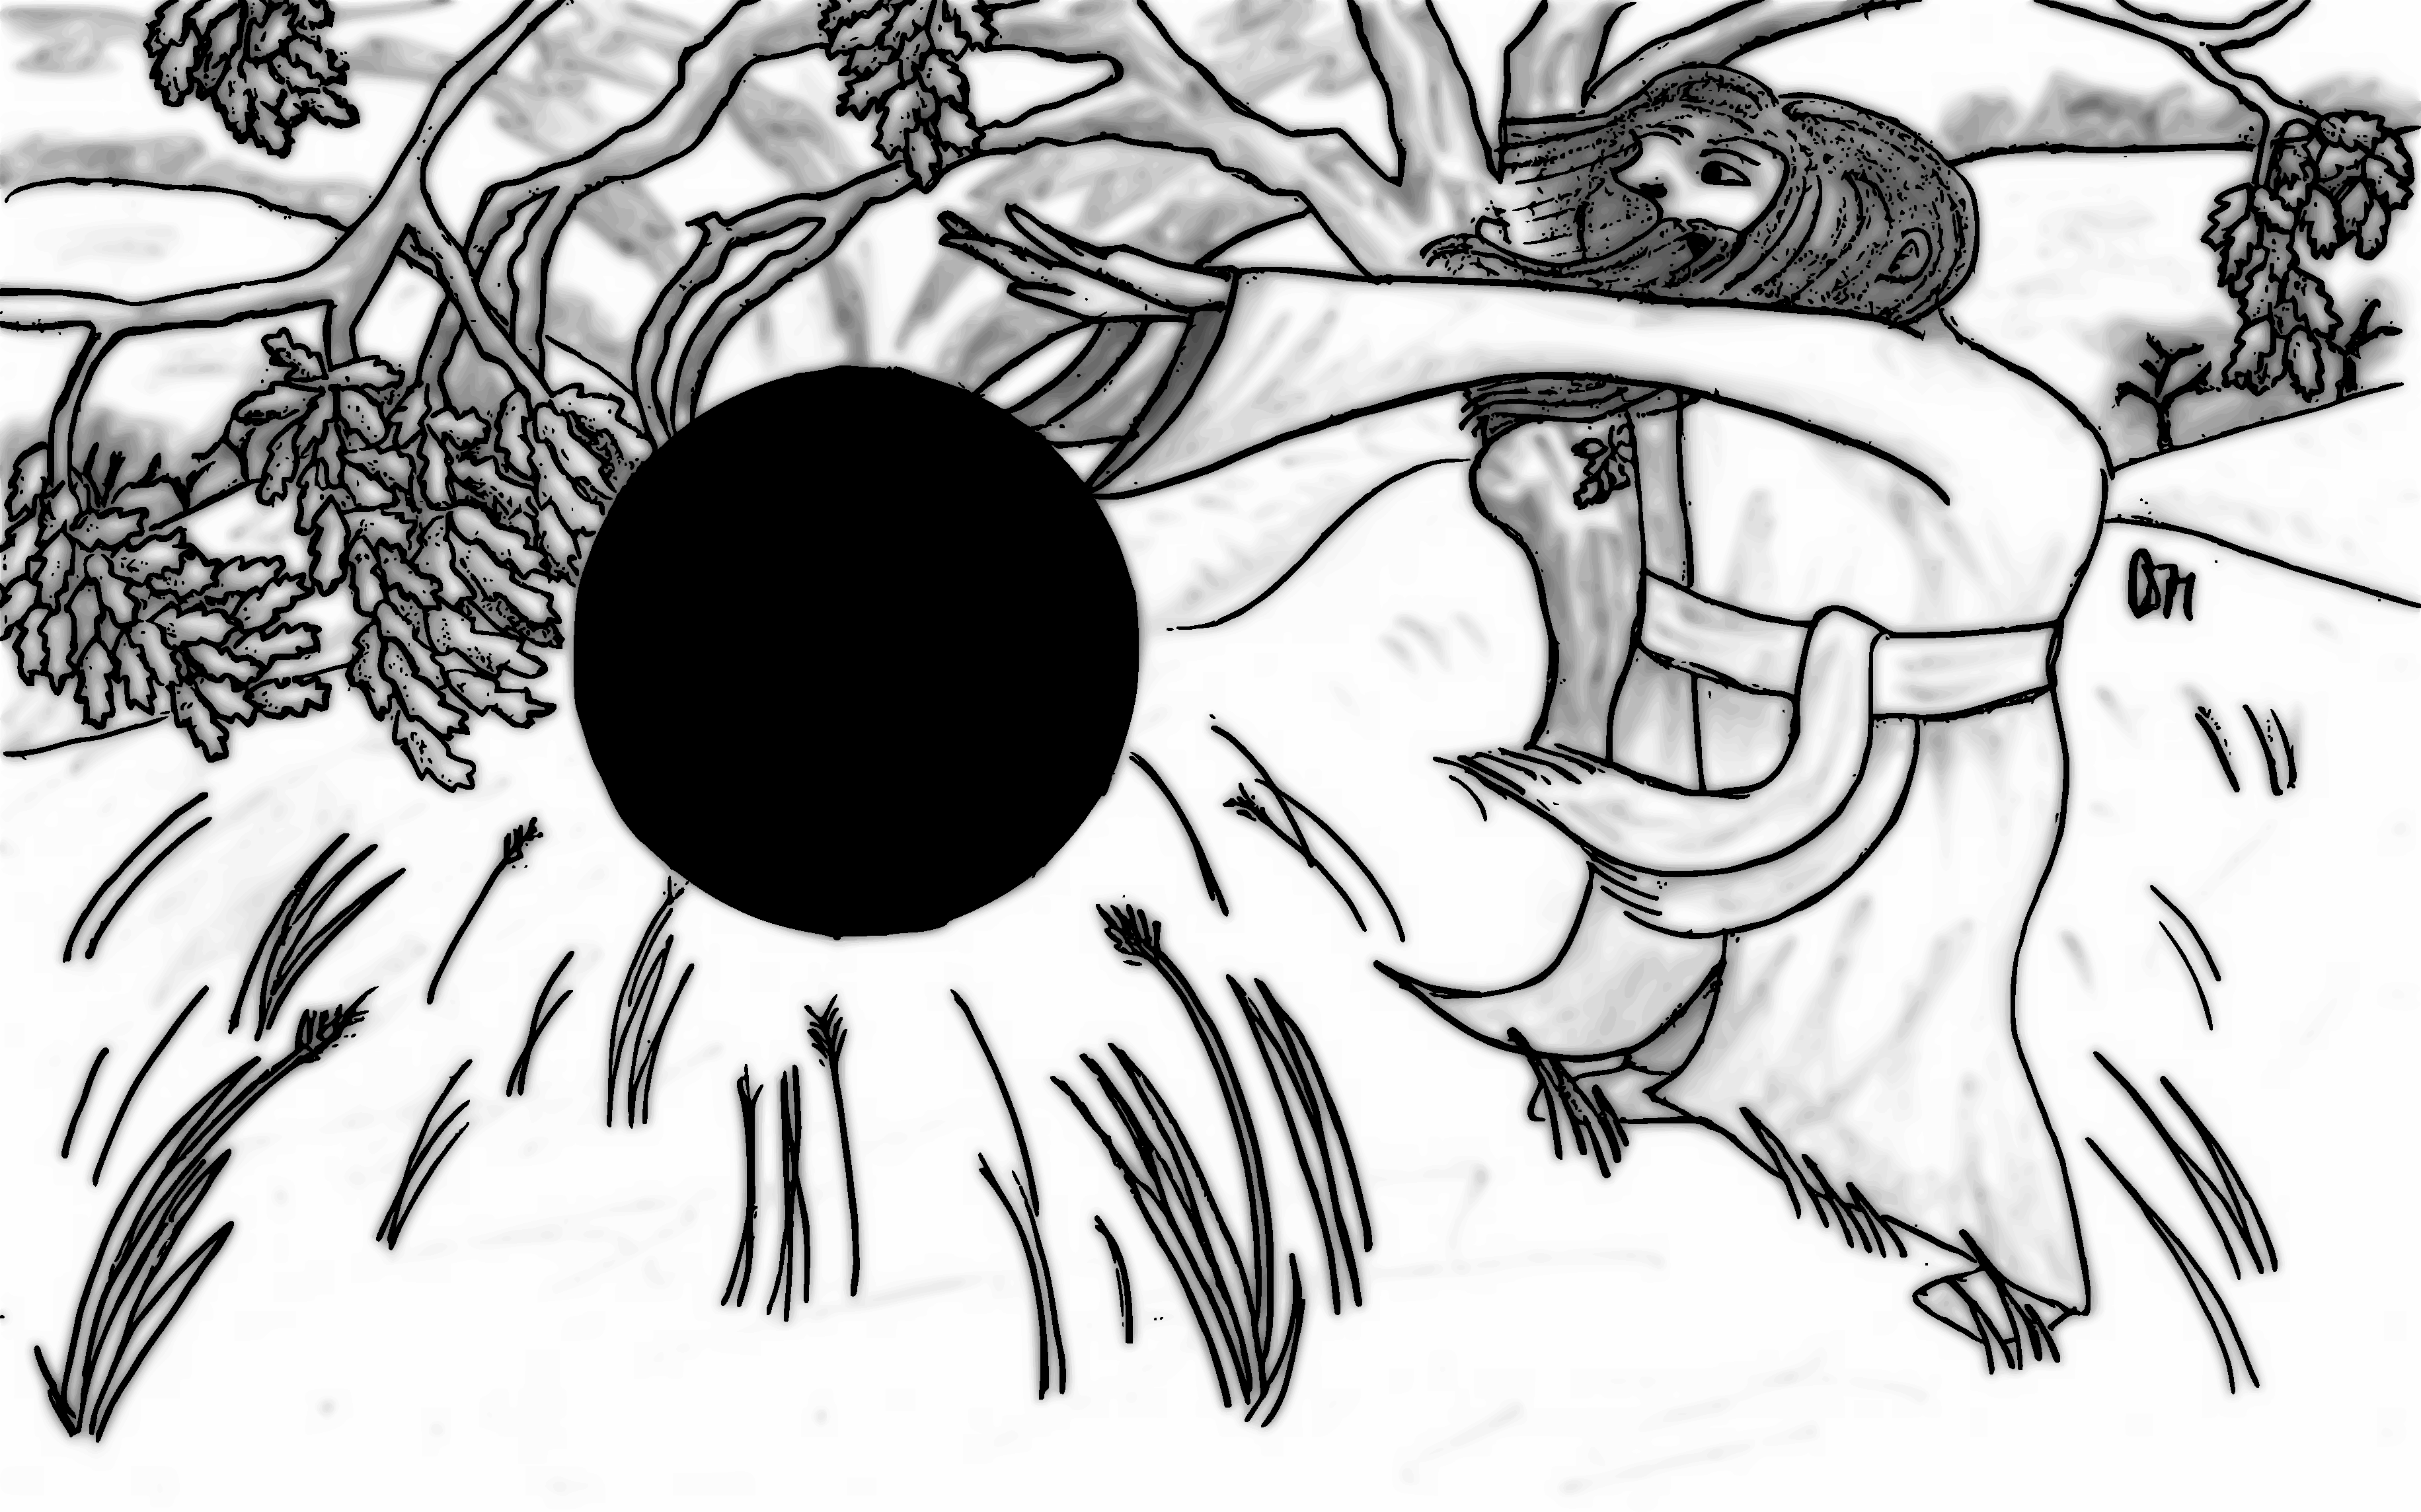
\includegraphics[width=0.95\columnwidth]{sphereofannihilation.pdf}\label{sphereofannihilation}

\end{center}

\paragraph{Sphere of Annihilation:} This magical sphere is a globe of absolute blackness, a ball of nothingness 2 feet in diameter.  The sphere has no mass or physical substance, so it has no gravity or other force of attraction, and is likewise unaffected by those forces.  When in static form, it remains in the same place relative to its surroundings.  The sphere radiates magic if \textit{detect magic} is cast, but it is actually a hole in the continuity of the multiverse.  Any matter that moves into contact with the sphere, or which the sphere moves into contact with, is instantly sent to Void-space: gone and utterly destroyed.  Void-space exists beyond the known limits of Dimensional Space.  

The sphere connects directly to Void-space, but its magic causes the pressure at its edge to equal the atmospheric or hydrostatic pressure outside.  This forms a pressure barrier permeable only by uniform motion on a macroscopic scale.  The random molecular motion of an atmospheric gas or liquid that usually surrounds a sphere does not break the pressure barrier; therefore a body of water or an atmosphere will flow around the sphere rather than be annihilated.  To cause the sphere to annihilate a gas or liquid, the substance can be blown or poured into the sphere, the sphere can be moved through the substance, or the sphere can be placed in front of a moving volume of a gas or liquid.    

A sphere cannot annihilate anything larger than 2' in diameter with a just single touch.  A sphere will bore a 2' diameter hole through a \textit{wall of force} or a physical wall such as a \textit{wall of stone}, \textit{wall or iron}, \textit{wall of ice}, etc. Hence, if a wizard controlling the sphere plunges it into the earth or into a castle wall, it bores a 2' hole instead of annihilating the entire item.  In a similar manner, a tiny-sized creature is small enough to be completely annihilated in one touch, but unless it falls completely into the sphere, a small-sized or larger creature may survive a single touch, suffering massive damage with up to a 2' section of their bodies missing.  Only the direct intervention of a deity can restore annihilated items or creatures, but lost limbs can be restored by a regenerate spell.  

If uncontrolled, the sphere is found in a motionless, static state, usually resting in mid-air.  However, by using mental effort to bend dimensional space around the sphere, any wizard, including specialty mages, can cause it to move.  In order to move the sphere, the wizard must first establish control over it.  Control of a sphere can be established from up to 40 feet away.  Once control is established, it can be maintained from a distance of 40 feet~+~10 feet per level of the wizard.  The sphere has a movement value based upon the level of the wizard controlling it, as shown on the table below.  The chance to establish control and maintain it each round is based on a combination of the wizard's intelligence and level. 
 
\noindent\begin{minipage}{\columnwidth} 
\noindent \begin{tabular}{|p{.3\columnwidth}|p{.3\columnwidth}|p{.25\columnwidth}|}
\hline
Wizard Level	& Movement Value	& Base Chance* \\
\hline\hline
\rowcolor[gray]{.9}up to 5\textsuperscript{th}	& 8'/round	& 15\% \\
6\textsuperscript{th} to 7\textsuperscript{th}	& 9'/round	& 20\% \\
\rowcolor[gray]{.9}8\textsuperscript{th} to 9\textsuperscript{th}	& 10'/round	& 30\% \\
10\textsuperscript{th} to 11\textsuperscript{th}	& 11'/round	& 40\% \\
\rowcolor[gray]{.9}12\textsuperscript{th} to 13\textsuperscript{th}	& 12'/round	& 50\% \\
14\textsuperscript{th} to 15\textsuperscript{th}	& 13'/round	& 60\% \\
\rowcolor[gray]{.9}16\textsuperscript{th} to 17\textsuperscript{th}	& 14'/round	& 70\% \\
18\textsuperscript{th} to 20\textsuperscript{th}	& 15'/round	& 75\% \\
\rowcolor[gray]{.9}21\textsuperscript{st}+	& 16'/round	& 80\% \\
\hline
\end{tabular}
\noindent\begin{tabular}{p{.95\columnwidth}}
*Every point of intelligence above 12 grants the wizard a 1\% bonus, increasing to 3\% for every point of intelligence above 15, up to a maximum of +12\% at intelligence 18. \\
\end{tabular}\vspace{.5em}
\end{minipage}

Simply attempting to establish control over the sphere sets it in motion.  If any attempt to establish or maintain control fails, the sphere uncontrollably pursues the wizard at the above listed movement value for at least 1d4 rounds.  Thereafter, the sphere continues to pursue the wizard if he remains within 30 feet of it.  If the wizard moves more than 30 feet away from it, the sphere becomes static again.  If the wizard has control over the sphere, he can command it to stop. 

If more than one wizard attempts to control the sphere simultaneously, they roll their checks in order from the wizard with the highest chance of success to the one with the lowest.  Each of their chances is reduced by 5\% per wizard attempting to control the sphere.  If all wizards fail their control checks, the sphere moves towards the one among them with the highest modified chance of success.  More than one wizard cannot cooperate to control a single sphere.

If a \textit{gate} spell is cast upon a sphere, there is a 50\% chance that the gate destroys the sphere in a harmless implosion, a 35\% chance that nothing happens, and a 15\% chance that a rip is opened through dimensional space, where everything within a 180-foot radius is sucked into the rip without benefit of a save and deposited onto another plane of existence, or possibly even somewhere as distant as an alternate multiverse.  

If a \textit{rod of cancellation} touches a sphere, they negate each other in a tremendous explosion.  Everything within a 60-foot radius takes 3d4 × 10 points of damage.  

These spheres are highly unpredictable, and the GM has several options in the unlikely event that two spheres are made to collide with each other.  The spheres may simply pass through each other as if the other was not there, they may merge and become a single larger sphere, or they may destroy each other.  Destruction of the spheres may result in a harmless implosion, a violent explosion, or a rip through dimensional space.  Similar results are possible if the sphere touches a \textit{bag of holding} or \textit{portable hole}.

A sphere will stop if it hits an \textit{anti-magic shell}, but \textit{dispel magic} and \textit{mage's disjunction} have no effect on it.  It is considered an artifact when subjected to any other effects.

\paragraph{Stone Horse:} This magical statue is crafted in the form of a life-sized figure of a horse. roughly hewn from some type of hard stone.  It radiates magic if \textit{detect magic} is cast.  When the command word is spoken, the statue animates but remains made of stone.   While animated, the statue is considered a construct against enchantment and illusionary effects, but makes any applicable saving throws against physical attacks as if it were a hard metal object.  Additionally, an animated statue can carry up to 1,000 pounds without encumbrance penalties and never requires water, food or rest.  

There are two known varieties of this statue:

\underline{The Courser:} When animated, this statue has a movement value of 24, AC 3, and 18 hit points.  It attacks as if it were a medium warhorse.

\underline{The Destrier:} When animated, this statue has a movement value of 18, AC 1, and 26 hit points.  It attacks as if it were a heavy warhorse.
 
If wounded or damaged, the statue can only be healed by casting \textit{transmute stone to flesh} upon it.  This transforms the statue into a living horse that radiates magic if \textit{detect magic} is cast.  While in flesh and blood form, it heals in the same manner as any real living creature, with a natural healing rate of 1 hit point per day.  When it is fully healed, it automatically returns to its non-animated statue form.  If the statue is destroyed or killed in any of its forms, it crumbles into dust.

\paragraph{Well of Many Worlds:} This strange, multi-dimensional device is crafted in the form of a \textit{portable hole} and radiates magic if \textit{detect magic} is cast.  When opened, the well establishes a direct connection to a randomly determined world anywhere within the multi-verse (another planet, a parallel Prime Material Plane, a different plane of existence, etc.), creating a two-way portal.  Anything entering the well is immediately transported to or from this other world.  It can be picked up, folded or rolled, just as a \textit{portable hole} can be, from either side of the portal.  However, if the center of the well is moved more than 3' away from its original position in any direction, a portal to another randomly determined world is created.  Once it is moved, the GM must decide whether placing the well within 3' of its original position will re-establish the link to the same world or not.  A return trip may prove to be difficult.

The well is reasonably stable, but under extraordinary circumstances (such as when a \textit{sphere of annihilation} enters the well or a creature casts a \textit{gate} upon it), the GM is free to determine the results as if it were a \textit{portable hole} or a \textit{sphere of annihilation}, as appropriate to the situation.

\paragraph{Wind Fan:} This magical fan is crafted in the form of a mundane, hand-held device used to create a cooling breeze.  It is usually made of wood and papyrus or cloth and painted with a colorfully detailed motif.  This fan radiates magic if \textit{detect magic} is cast, but is fragile with poor saving throws, especially vs. fire-based attacks.  If damaged in any way, it becomes a mundane item. 

By uttering the command word, its user causes the fan to generate air movement duplicating a \textit{gust of wind} spell cast by a 5\textsuperscript{th} level spell caster.  The fan can be used once per day with no risk.  If it is used more frequently, there is a 20\% cumulative chance per usage during that day that the device is damaged and becomes useless mundane tatters.

\paragraph{Wings of Flying:} This magical pair of wings is usually crafted in the form of a plain cloak made of common black cloth, but more exotic varieties may exist that are in the form of a long, elegant cape of feathers.  Once per day, the wearer can speak a command phrase to cause the cloak to turn into a gigantic pair (20-foot wing span) of bat or bird wings that allow the wearer and anything that he wears or carries (up to 500 total pounds) to fly.  As part of the command phrase, the wearer must include the maximum flight duration that the wings will remain active.  The specified flight duration indicates the wearer's maximum flight speed as shown on the following table.

\noindent \begin{tabular}{|p{.3\columnwidth}|p{.25\columnwidth}|p{.3\columnwidth}|}
\hline
Flight Duration	& Max Speed	& Speed Class \\
\hline\hline
\rowcolor[gray]{.9}2 turns	& 32	& 3---quick \\
3 turns	& 25	& 3---quick \\
\rowcolor[gray]{.9}4 turns	& 18	& 2---average \\
6 turns	& 15	& 2---average \\
\rowcolor[gray]{.9}8 turns	& 12	& 1---slow \\
\hline
\end{tabular}

The wings give their wearer maneuver class 3 (average).  He can use a weapon, shield or magical item while flying, but cannot cast spells or concentrate on controlling magical effects.  If the wearer lands for any reason, the wings return to the form of a cloak and the flight duration ends early.  

Flights lasting longer than one turn fatigue the wearer.  If the flight lasts more than a turn, the wearer can only move at $^1$/$_2$ his normal movement rate or slower for one hour.  If the flight lasts for the entire duration, the wearer must stop moving and rest, relax and/or sleep for one hour. 

\section{MAGICAL ARMOR \& SHIELDS}

\index{Armor!Magical Armor}\index{Magical Armor}Magical armor is 65\% likely to be man-sized, 20\% likely to be elf-sized, 10\% to be dwarf-sized, and 5\% to be gnome-sized or halfling-sized, unless specified in its description.  On the other hand, it may be assumed that magical armor can be adjusted to fit a variety of wearers, so a more lenient system would allow 85\% to fit any basically human-sized creature, including elves, half-elves and dwarves, while the remaining 15\% would fit any small-sized creature such as gnomes and halflings. The GM always has the option to use a different set of percentage chances to represent his particular campaign setting. 

Magical armor and shields radiate magic if \textit{detect magic} is cast and grant the wearer an enchantment bonus between +1 and +5.  The armor or shield's AC modifier is improved (i.e. lowered) by this amount.  Regardless of magical equipment or bonuses, the best AC a creature can have is $-10$; however, situational modifiers could still provide penalties to hit a creature with AC $-10$ when applicable.  

\index{Cursed Armor}Most accursed armor and shields radiate magic if \textit{detect magic} is cast but inflict AC penalties expressed as negative numbers. The armor or shield's AC modifier is decreased (i.e. raised) by this amount.  Regardless of magical equipment or bonuses, the worst AC a creature can have is 10; however, situational modifiers could still provide bonuses to hit the creature with AC 10 when applicable.  

Refer to Modifying Saving Throws for when to apply a magical armor's enchantment bonus (or an accursed armor's enchantment penalty) to its wearer's saving throws.

Magical armor weighs the same as mundane armor of the same type, but when worn its weight only counts toward a creature's strength-max weight score.  It is considered weightless when determining whether the creature wearing it suffers any encumbrance related penalties (refer to Encumbrance).  

To determine the type of magical armor or shield found, roll on Table B.44: Armor Type and determine its enchantment bonus (or penalty) by rolling on Table B.45: Enchantment Modifier.  

\noindent \begin{minipage}{\columnwidth}

\captionof{table}{Armor Type}\label{armortype}
\noindent \begin{tabular}{|p{.15\columnwidth}|p{.75\columnwidth}|}
\hline
1d20	& Armor \\
\hline\hline
\rowcolor[gray]{.9}1	& Banded mail \\
2	& Brigandine \\
\rowcolor[gray]{.9}3--5	& Chain mail \\
6	& Field plate \\
\rowcolor[gray]{.9}7	& Full plate \\
8	& Leather or padded \\
\rowcolor[gray]{.9}9--12	& Plate mail \\
13	& Plate mail (bronze) \\
\rowcolor[gray]{.9}14	& Scale mail \\
15--17	& Shield \\
\rowcolor[gray]{.9}18	& Splint mail \\
19	& Studded leather \\
\rowcolor[gray]{.9}20	& Special* \\
\hline
\end{tabular}
\noindent\begin{tabular}{p{.95\columnwidth}}
*Roll on Table \ref{specialarmors}: Special Armors. \\
\end{tabular}\vspace{.5em}

\end{minipage}

\noindent \begin{minipage}{\columnwidth}

\captionof{table}{Enchantment Modifier}\label{armorenchant}

\noindent \begin{tabular}{|p{.3\columnwidth}|p{.25\columnwidth}|p{.3\columnwidth}|}
\hline
1d20	& AC Adj.	& XP \\
\hline\hline
\rowcolor[gray]{.9}1--2	& $-1$	& Cursed \\
3--10	& +1	& 500 \\
\rowcolor[gray]{.9}11--14	& +2	& 1,000 \\
15--17	& +3	& 1,500 \\
\rowcolor[gray]{.9}18--19	& +4	& 2,000 \\
20	& +5	& 3,000 \\
\hline
\end{tabular}

\end{minipage}

\noindent \begin{minipage}{\columnwidth}

\captionof{table}{Special Armors}\label{specialarmors}

\noindent \begin{tabular}{|p{.15\columnwidth}|p{.5\columnwidth}|p{.2\columnwidth}|}
\hline
1d20	& Armor Type	& XP \\
\hline\hline
\rowcolor[gray]{.9}1--2	& Armor of Blending	& +500* \\
3--4	& Armor of Command	& +1,000* \\
\rowcolor[gray]{.9}5--6	& Armor of Missile Attraction	& Accursed \\
7--8	& Armor of Rage	& Accursed \\
\rowcolor[gray]{.9}9--10	& Elven Chain Mail	& ** \\
11--12	& Plate Mail of Etherealness	& 5,000 \\
\rowcolor[gray]{.9}13--14	& Plate Mail of Fear	& 4,000 \\
15--16	& Plate Mail of Vulnerability	& Accursed \\
\rowcolor[gray]{.9}17--18	& +1 Large shield, +4 vs. missiles	& 400 \\
19--20	& $-1$ Shield, missile attractor	& Accursed \\
\hline
\end{tabular}
\noindent\begin{tabular}{p{.95\columnwidth}}
*This experience is added to that from the armor's enchantment bonus. \\
**Refer to the item's description. \\
\end{tabular}\vspace{.5em}

\end{minipage}

\subsection{SPECIAL ARMOR DESCRIPTIONS}

\index{Armor!Magical Armor!Special Armor}Magical armor and shields that have additional powers are further described below.

\paragraph{Armor of Blending:} This magical armor is crafted in all combinations of mundane armor type and enchantment bonus (roll for type of armor and enchantment modifier, ignoring enchantment penalties).  It radiates magic if \textit{detect magic} is cast.  Speaking a command word causes the armor to disguise itself as mundane clothing.  The power is merely illusory in nature, and the armor retains all of its normal properties while disguised.  Only \textit{true seeing} (or similar effect) will reveal the disguised armor's true nature.

\paragraph{Armor of Command:} This magical armor can be crafted in any combination of mundane armor type and enchantment bonus (roll for type of armor and enchantment modifier, ignoring enchantment penalties), but it is obviously finely crafted and radiates a strong aura of magic if \textit{detect magic} is cast.  This armor has the power to grant its wearer a charisma score of 18 for the purposes of determining encounter reactions.  Racial modifiers may still apply.  If the wearer's charisma is already higher than or equal to 18, nothing is gained or lost.  In addition, allies within 360 feet of the wearer gain a +2 bonus to their morale score (PCs are not affected by this morale bonus).  The morale bonus is lost if the wearer hides or conceals himself in any way.  If a bard wears this armor, he is empowered with the ability to cast a \textit{command} spell once per day.  

\paragraph{Armor of Missile Attraction:} This accursed armor can be crafted in any combination of mundane armor type and enchantment bonus (roll for type of armor and enchantment modifier, ignoring enchantment penalties).  It radiates magic if \textit{detect magic} is cast and acts as an ordinary set of magical armor until hostile opponents are encountered.  Its curse then attracts missile weapons to the wearer's location.  The wearer is at least twice as likely to be a randomly selected target if missiles are fired into a crowd.  In mass combat situations where volleys of missiles are fired, the wearer always has the most missiles fired in his direction. Furthermore, the armor provides no enchantment bonus against such weapons.  Simple tests won't reveal its cursed nature.  Only a \textit{remove curse} spell allows the armor to be removed once the curse has been discovered.

\paragraph{Armor of Rage:} This accursed armor is crafted in the form and function of \textit{armor of command}, including granting its wearer an enchantment bonus.  However, its primary effect on people is quite the opposite.  When worn, the wearer suffers a $-3$ penalty to all charisma related encounter checks.  Allies within 360 feet of the wearer suffer a $-2$ penalty to their morale score (PCs are not affected by this morale penalty).  The curse is subtle and not immediately evident to the wearer or those affected.  Only a \textit{remove curse} spell allows the armor to be removed once the curse has been discovered.

\paragraph{Elven Chain Mail:} This magical armor is crafted in the form of finely made chain mail.  It radiates magic if \textit{detect magic} is cast and provides an enchantment bonus (roll for an enchantment modifier, ignoring enchantment penalties).  This armor is incredibly light and can be worn under normal clothing without revealing its presence.  Rogues can wear it, suffering only a few penalties to their class abilities, and elven fighter/mages can cast spells while wearing it without restriction.  The extremely rare armor can only be crafted by elves and is almost always custom made for an individual.  Therefore, it is rarely sized to fit anyone other than an elf or half-elf.

\noindent \begin{tabular}{|p{.15\columnwidth}|p{.75\columnwidth}|}
\hline
1d100	& Size \\
\hline\hline
\rowcolor[gray]{.9}01--10	& gnome/halfling \\
11--15	& dwarf \\
\rowcolor[gray]{.9}16--80	& elf/half-elf \\
81--95	& man-sized, up to 6' and 200 lbs. \\
\rowcolor[gray]{.9}96--00	& man-sized, up to 6.5' and 250 lbs. \\
\hline
\end{tabular}

The experience points rewarded for finding a suit of this armor is listed below.  This reflects the item's unique properties, value and rarity.
 
\noindent \begin{tabular}{|p{.45\columnwidth}|p{.45\columnwidth}|}
\hline
Bonus	& Exp \\
\hline\hline
\rowcolor[gray]{.9}+1	& 1,200 \\
+2	& 2,000 \\
\rowcolor[gray]{.9}+3	& 3,000 \\
+4	& 5,000 \\
\rowcolor[gray]{.9}+5	& 7,500 \\
\hline
\end{tabular}

\paragraph{Plate Mail of Etherealness:} This magical armor is crafted in the form and function of \textit{+5 plate mail}.  It radiates magic if \textit{detect magic} is cast, and upon command, its power allows the wearer and any nonliving items he wears and carries to become ethereal as if an \textit{oil of etherealness} had been applied.  While on the Ethereal Plane, the wearer cannot attack creatures on the Prime Material Plane.  A \textit{phase door} spell cast upon the wearer from either plane cancels the armor's power to remain ethereal, returning him and his gear to the Prime Material Plane (as applicable) and preventing the armor's power of etherealness from functioning for one full day.

Each suit of armor is crafted with 20 charges and cannot be recharged.  Each visit to the Ethereal Plane expends one charge.  Expending five charges reduces the armor's enchantment bonus by 1, until all 20 charges are expended and it becomes an ordinary suit of +1 plate mail.  As with all charged magical items, the armor may not have its full amount of charges when found, depending upon the frequency of its use by its former owner(s).

\paragraph{Plate Mail of Fear:}  This magical armor is crafted in the form and function of +1 plate mail.  It radiates magic if \textit{detect magic} is cast, and upon command, the armor radiates fear in a 30 foot radius.  All creatures in the effective area, except the wearer, must roll a successful save vs. spell or panic.  Those who fail their save run away from the wearer (or cower if backed into a corner) for 1d4~+~1 rounds.  

Each suit of armor is crafted with 2d2~+~3 charges.  Activating the fear aura expends one charge.  The armor cannot be recharged, but retains its +1 enchantment bonus even after all charges are expended.  As with all charged magical items, the armor may not have its full amount of charges when found, depending upon the frequency of its use by its former owner(s).

\paragraph{Plate Mail of Vulnerability:} This accursed armor is crafted in the form and function of ordinary magical plate mail.  It radiates magic if \textit{detect magic} is cast and initially provides an enchantment bonus (roll for an enchantment modifier, ignoring enchantment penalties).  However, when a hostile opponent strikes the wearer in battle, the armor's curse activates and its enchantment bonus reverses to apply a penalty to the wearer's AC and any applicable saving throws.  If a hostile opponent hits the wearer with a natural 20 on his attack roll, the armor shatters.  Otherwise, only a \textit{remove curse} spell allows the armor to be removed once the curse has been discovered 

\paragraph{+1 Large shield, +4 vs. missiles:} This large shield grants a +1 enchantment bonus to its bearer's AC against melee attacks and a +4 enchantment bonus against missile or hurled weapons.  In addition, the shield has a 20\% chance to negate \textit{magic missile} spells that target the bearer from either the front or rear, depending on how the shield is carried.

\paragraph{$-1$ Shield, missile attractor:} This accursed shield is crafted in the form and function of an ordinary +1 shield.  It radiates magic if \textit{detect magic} is cast and acts as an ordinary magical shield until hostile opponents are encountered.  Its curse then attracts missile weapons to the wearer's location.  The wearer is at least twice as likely to be a randomly selected target if missiles are fired into a crowd.  In mass combat situations where volleys of missiles are fired, the wearer always has the most missiles fired in his direction. Furthermore, the shield inflicts an enchantment penalty of $-1$ to the wearer's AC against all weapons, effectively canceling the shield's mundane bonus.   Simple tests won't reveal its cursed nature.  The shield will remain in its bearer's possession, reappearing if discarded or destroyed, until a \textit{remove curse} spell is cast upon it.

%\vspace{1em}

%\noindent
\includegraphics[width=\columnwidth]{axe2e.pdf}\label{axe2e}
 
\section{MAGICAL WEAPONS}

\index{Magical Weapons}\index{Weapons!Magical Weapons}Normal magical weapons radiate magic if \textit{detect magic} is cast and carry an enchantment bonus of between +1 and +5, which is added to the weapon's attack rolls and damage scores. However, it is unusual for any weapon other than a sword to carry an enchantment bonus of greater than +3.  

\index{Cursed Weapons}Most accursed weapons radiate magic if \textit{detect magic} is cast, but carry an enchantment penalty of between $-1$ and $-5$, which is subtracted from the weapon's attack rolls and damage scores. An accursed weapon's damage cannot be reduced below 1 hit point.  

Some special magical weapons specifically state whether or not they glow or otherwise give off light in their description.  Otherwise, the GM may determine that certain other magical weapons glow on a case-by-case basis, including swords, daggers, and any weapon with a +3 or higher enchantment bonus.  If a weapon is said to glow, it will shed light in a 5' radius whenever it is removed from its sheath.  The weapon will not glow until its wielder discovers that it is magical, but once the glow is activated, it cannot be deactivated until a new owner who is unaware of its power picks it up.

Magical swords are the most commonly found magical weapons and come in the greatest number of varieties.  Unless otherwise stated in the sword's description, 70\% of all known magical swords are long swords, 20\% are scimitars or broad swords (50\% chance for either), 5\% are short swords, 4\% are bastard swords, and 1\% are two-handed swords.  

When a magical weapon other than a sword is rolled that is commonly found in more than one variety, such as a mace, a flail, a pole arm, or a group of arrows or bolts, etc., the GM must determine the most appropriate weapon for the situation.  For example, if encountering a mounted warrior with a magical mace, it is likely that the mace is of the horseman's variety, while a warrior on foot would more likely be carrying a magical footman's mace.

Magical lances are almost always heavy lances.  
 
Ordinary magical hand-axes can be hurled with normal ranges, but when hurled they only add their enchantment bonus to their attack rolls, and not to their damage scores.  

Magical spears and arrows follow the same rules as their mundane counterparts (refer to Mundane Weapons \& Armor).

If two opponents wield weapons that allow them to strike before initiative is rolled, they attack each other simultaneously.

To determine the type of magical weapon found, roll on Table B.47: Weapon Type and determine its enchantment bonus (or penalty) by rolling on Table B.48: Enchantment Modifier.

\noindent \begin{minipage}{\columnwidth}

\captionof{table}{Weapon Type (1d6)}\label{weapontype}
\noindent \begin{tabular}{|p{.15\columnwidth}|p{.75\columnwidth}|}
\multicolumn{2}{c}{Sub-Table A (1--2)} \\
\hline
1d20	& Weapon (Quantity) \\
\hline\hline
\rowcolor[gray]{.9}1	& Arrow (4d6) \\
2	& Arrow (3d6) \\
\rowcolor[gray]{.9}3	& Arrow (2d6) \\
4--5	& Axe, Hand or Throwing \\
\rowcolor[gray]{.9}6	& Battle axe \\
7	& Bolt (2d10) \\
\rowcolor[gray]{.9}8	& Bolt (2d6) \\
9	& Bullet, Sling (3d4) \\
\rowcolor[gray]{.9}10--12	& Dagger \\
13	& Dart (3d4) \\
\rowcolor[gray]{.9}14	& Flail \\
15	& Javelin (1d2) \\
\rowcolor[gray]{.9}16	& Knife \\
17	& Lance \\
\rowcolor[gray]{.9}18--19	& Mace \\
20	& Special* \\
\hline
\end{tabular}

\end{minipage}

\noindent \begin{tabular}{|p{.15\columnwidth}|p{.75\columnwidth}|}
\multicolumn{2}{c}{Sub-Table B (3--6)} \\
\hline
1d20	& Weapon \\
\hline\hline
\rowcolor[gray]{.9}1	& Military Pick \\
2	& Morning Star \\
\rowcolor[gray]{.9}3	& Pole Arm or Pole Axe \\
4--5	& Scimitar \\
\rowcolor[gray]{.9}6--8	& Spear \\
9--17	& Sword \\
\rowcolor[gray]{.9}18	& Trident \\
19	& War Hammer \\
\rowcolor[gray]{.9}20	& Special* \\
\hline
\end{tabular}
\noindent\begin{tabular}{p{.95\columnwidth}}
*Roll on Table \ref{specialweapons}: Special Weapons. \\
\end{tabular}\vspace{.5em}
 
\noindent \begin{minipage}{\columnwidth}

\captionof{table}{Enchantment Modifier}\label{weaponenchantment}
\noindent \begin{tabular}{|p{.15\columnwidth}|p{.15\columnwidth}|p{.15\columnwidth}|p{.15\columnwidth}|p{.15\columnwidth}|}
\hline
1d20	& Sword	& XP	& Other	& XP \\
\hline\hline
\rowcolor[gray]{.9}1--2	& $-1$	& Cursed	& $-1$	& Cursed \\
3--10	& +1	& 400	& +1	& 500 \\
\rowcolor[gray]{.9}11--14	& +2	& 800	& +1	& 500 \\
15--17	& +3	& 1,400	& +2	& 1,000 \\
\rowcolor[gray]{.9}18--19	& +4	& 2,000	& +2	& 1,000 \\
20	& +5	& 3,000	& +3	& 2,000 \\
\hline
\end{tabular}

\end{minipage}
 
\noindent \begin{minipage}{\columnwidth}

\captionof{table}{Special Weapon (1d10)}\label{specialweapons}
\noindent \begin{tabular}{|p{.12\columnwidth}|p{.55\columnwidth}|p{.18\columnwidth}|}
\multicolumn{3}{c}{Sub-Table A (1--3)} \\
\hline
1d20	& Item	& XP \\
\hline\hline
\rowcolor[gray]{.9}1	& Arrow of Direction	& 2,500 \\
2	& +3 Arrow of Slaying	& 250 \\
\rowcolor[gray]{.9}3	& +2 Axe of Far Throwing	& 750 \\
4	& Axe of Return	& * \\
\rowcolor[gray]{.9}5--6	& +1 Bow	& 500 \\
7	& +3 Crossbow of Accuracy	& 2,000 \\
\rowcolor[gray]{.9}8	& +1 Crossbow of Distance	& 1,500 \\
9	& +1 Crossbow of Speed	& 1,500 \\
\rowcolor[gray]{.9}10--11	& +1 Dagger, +2 vs. Small-sized or Smaller Creatures	& 300 \\
12--13	& +2 Dagger, +3 vs. Large-sized or Larger Creatures	& 300 \\
\rowcolor[gray]{.9}14	& +2 Dagger, Long Tooth	& 300 \\
15	& Dagger of Throwing	& * \\
\rowcolor[gray]{.9}16	& +1 Dagger of Venom	& 350 \\
17	& +3 Dart of Homing	& 450 \\
\rowcolor[gray]{.9}18	& +2 Hammer, +3 Dwarven Thrower	& 1,500 \\
19	& Hammer of Thunderbolts	& 2,500 \\
\rowcolor[gray]{.9}20	& GM's Choice	& -- \\
\hline
\end{tabular}
\noindent\begin{tabular}{p{.95\columnwidth}}
*Refer to the item's description \\
\end{tabular}\vspace{.5em}

\end{minipage}

\noindent \begin{tabular}{|p{.12\columnwidth}|p{.55\columnwidth}|p{.18\columnwidth}|}
\multicolumn{3}{c}{Sub-Table B (4--6)} \\
\hline
1d20	& Item	& XP \\
\hline\hline
\rowcolor[gray]{.9}1	& Horn Blade	& * \\
2	& Javelin of Lightning	& 250 \\
\rowcolor[gray]{.9}3	& +6 Javelin of Piercing	& 250 \\
4--5	& Knife, Buckle	& 150 \\
\rowcolor[gray]{.9}6--7	& +1 Mace of Disruption	& 2,000 \\
8	& Net of Entrapment	& 1,000 \\
\rowcolor[gray]{.9}9	& Net of Snaring	& 1,000 \\
10--11	& Quarterstaff, Magical	& 500 \\
\rowcolor[gray]{.9}12	& Scimitar of Speed	& * \\
13--14	& +2 Sling of Seeking	& 700 \\
\rowcolor[gray]{.9}15	& Spear, Backbiter	& Accursed \\
16	& +1 Trident of Fish Command	& 500 \\
\rowcolor[gray]{.9}17	& +1 Trident of Submission	& 1,500 \\
18	& +2 Trident of Warning	& 1,000 \\
\rowcolor[gray]{.9}19	& $-2$ Trident of Yearning	& Accursed \\
20	& GM's Choice	& -- \\
\hline
\end{tabular}
\noindent\begin{tabular}{p{.95\columnwidth}}
* See item's description \\
\end{tabular}\vspace{.5em}

\noindent \begin{tabular}{|p{.12\columnwidth}|p{.55\columnwidth}|p{.18\columnwidth}|}
\multicolumn{3}{c}{Sub-Table C (7--9)} \\
\hline
1d20	& Item	& XP \\
\hline\hline
\rowcolor[gray]{.9}1	& +2 Sword, Sun Blade	& 3,000 \\
2--7	& +1 Sword, Mage Bane	& 600 \\
\rowcolor[gray]{.9}8--10	& +1 Sword, Morph Dropper	& 700 \\
11--12	& +1 Sword, Rejuvenator Slayer	& 800 \\
\rowcolor[gray]{.9}13	& +1 Sword, Lizard Killer	& 800 \\
14--15	& +1 Sword, Cursed	& Accursed \\
\rowcolor[gray]{.9}16	& +1 Sword, Flame Tongue	& 900 \\
17	& +1 Sword, Luck Blade	& 1,000 \\
\rowcolor[gray]{.9}18	& +2 Sword, Dragon Slayer	& 900 \\
19	& +2 Sword, Giant Slayer	& 900 \\
\rowcolor[gray]{.9}20	& GM's Choice	& -- \\
\hline
\end{tabular}

\noindent \begin{tabular}{|p{.12\columnwidth}|p{.55\columnwidth}|p{.18\columnwidth}|}
\multicolumn{3}{c}{Sub-Table D (10)} \\
\hline
1d20	& Item	& XP \\
\hline\hline
\rowcolor[gray]{.9}1	& +2 Sword, Nine Lives Stealer	& 1,600 \\
2--3	& +3 Sword, Frost Brand	& 1,600 \\
\rowcolor[gray]{.9}4	& +4 Sword, Defender	& 3,000 \\
5	& +5 Sword, Defender	& 3,600 \\
\rowcolor[gray]{.9}6	& +5 Sword, Holy Avenger	& 4,000 \\
7--8	& $-2$ Sword, Cursed	& Accursed \\
\rowcolor[gray]{.9}9	& +1 Sword of Dancing	& 4,400 \\
10	& +2 Sword of Life Stealing	& 5,000 \\
\rowcolor[gray]{.9}11	& +1 Sword of Sharpness	& 7,000 \\
12	& +1 Sword of the Planes	& 2,000 \\
\rowcolor[gray]{.9}13	& +1 Sword of Wounding	& 4,400 \\
14--16	& +2 Sword, Cursed Berserking	& Accursed \\
\rowcolor[gray]{.9}17--18	& +2 Short Sword of Quickness	& 1,000 \\
19	& +3 Sword, Vorpal	& 10,000 \\
\rowcolor[gray]{.9}20	& GM's Choice	& -- \\
\hline
\end{tabular}

\index{Weapons!Magical Weapons!Special Weapons}\subsection{SPECIAL WEAPON DESCRIPTIONS}

\paragraph{Arrow of Direction:} This magical arrow is crafted in the form of a mundane arrow, but radiates magic if \textit{detect magic} is cast.  It rarely carries an enchantment bonus but has a power similar to that of the \textit{locate object} spell.  Once per day, the owner of the arrow can activate the arrow by requesting the location of one of the following specific types of areas: a stairway (up or down), a sloping passage (up or down), an exit or entrance to a dungeon, or a cave or cavern.  The request must also include relative distance (nearest, farthest, highest, lowest) and/or direction (north, south, east, west, etc.).  The arrow is then tossed into the air and when it falls to the ground it points towards the requested area.  Once activated, the arrow can be tossed into the air up to seven times within seven turns or until the area is found.

\paragraph{+3 Arrow of Slaying:}  This magical arrow is crafted in many exotic forms indicative of the specific type of creature that it is intended to slay.  In addition to special materials, rare feathers, specially shaped heads and intricately carved runes, an arrow of this sort will radiate magic if \textit{detect magic} is cast and carries a +3 enchantment bonus.  There are many varieties of these magical arrows, and each is enchanted to instantly kill a specific type of creature without benefit of a saving throw, upon a successful hit.  Some possibilities include:

\noindent \begin{tabular}{|p{.45\columnwidth}|p{.45\columnwidth}|}
\hline
1d20	& Type \\
\hline\hline
\rowcolor[gray]{.9}1	& Arachnids \\
2	& Avians \\
\rowcolor[gray]{.9}3	& Bards \\
4	& Clerics \\
\rowcolor[gray]{.9}5	& Dragons \\
6	& Druids \\
\rowcolor[gray]{.9}7	& Elementals \\
8	& Fighters \\
\rowcolor[gray]{.9}9	& Giants \\
10	& Golems \\
\rowcolor[gray]{.9}11	& Illusionists \\
12	& Mages \\
\rowcolor[gray]{.9}13	& Mammals \\
14	& Paladins \\
\rowcolor[gray]{.9}15	& Rangers \\
16	& Reptiles \\
\rowcolor[gray]{.9}17	& Sea monsters \\
18	& Thieves \\
\rowcolor[gray]{.9}19	& Titans \\
20	& Undead \\
\hline
\end{tabular}

The GM is encouraged to customize this table for his campaign world.

\paragraph{+2 Axe of Far Throwing:} This magical axe is crafted either in the form of a mundane hand axe or a normal, magical \textit{+2 hand axe}.  However, it can be hurled up to 180 feet, and adds its enhancement bonus to both attack rolls and damage scores when hurled.

\paragraph{Axe of Return:} This magical axe is crafted either in the form of a mundane hand axe or a normal magical hand axe, but has an enchantment bonus as determined on the table below.  Like an \textit{axe of far throwing}, it can be hurled up to 180 feet. When hurled, a successful hit inflicts double the base damage (2d6 or 2d4), in addition to its enchantment bonus.  The axe then returns to the wielder's hand in the same round it is hurled regardless if it hits or misses its target.  If the wielder of the axe is unaware of its power to return, he gains a cumulative 1 in 8 chance each consecutive week that he wields the axe to discover the power.  The weapon's power will be revealed automatically after eight weeks of consecutive use.

\noindent \begin{tabular}{|p{.3\columnwidth}|p{.3\columnwidth}|p{.25\columnwidth}|}
\hline
1d20	& Bonus	& XP \\
\hline\hline
\rowcolor[gray]{0.9}1--5	& +1	& 1,500 \\
6--10	& +2	& 3,000 \\
\rowcolor[gray]{0.9}11--15	& +3	& 4,500 \\
16--19	& +4	& 6,000 \\
\rowcolor[gray]{0.9}20	& +5	& 7,500 \\
\hline
\end{tabular}

\paragraph{+1 Bow:} This magical bow can be crafted in the form of any mundane type of bow (composite, short, or long) as desired by the GM, but radiates magic if \textit{detect magic} is cast.  Its enchantment bonus applies to its attack rolls and damage scores of arrows that are fired from it.  If magical arrows are fired, the enchantment bonuses from both weapons are combined.  A mundane arrow fired from a magical bow is not considered a magical weapon.

\paragraph{+3 Crossbow of Accuracy:} This magical crossbow is most often crafted in the form of a mundane light crossbow, with only 10\% crafted in the form of a heavy crossbow.  It radiates magic if \textit{detect magic} is cast and suffers no THACO penalty when fired at medium or long ranges.  Its enchantment bonus is applied to its attack rolls (but not its damage scores).  If magical bolts are fired, the enchantment bonuses from both weapons are combined.  A mundane bolt fired from a magical crossbow is not considered a magical weapon.

\paragraph{Crossbow of Distance:} This magical crossbow is most often crafted in the form of a mundane light crossbow, with only 10\% crafted in the form of a heavy crossbow.  It radiates magic if \textit{detect magic} is cast, and its power doubles the weapon's short, medium, and long ranges.  Its enchantment bonus applies to its attack rolls and damage scores of bolts that are fired from it.  If magical bolts are fired, the enchantment bonuses from both weapons are combined.  A mundane bolt fired from a magical crossbow is not considered a magical weapon.

\paragraph{+1 Crossbow of Speed:} This magical crossbow is most often crafted in the form of a mundane light crossbow, with only 10\% crafted in the form of a heavy crossbow.  It radiates magic if \textit{detect magic} is cast, and its power doubles the weapon's rate of fire.    When grasped, the crossbow also automatically cocks itself and allows the wielder to fire first (and last, as applicable) in a melee round, except when he is surprised.  Its enchantment bonus applies to its attack rolls and damage scores of bolts that are fired from it.  If magical bolts are fired, the enchantment bonuses from both weapons are combined.  A mundane bolt fired from a magical crossbow is not considered a magical weapon.

\paragraph{+2 Dagger, Long Tooth:} This magical dagger can be crafted in the form of either a mundane dagger or a normal \textit{+2 dagger}.  When wielded by a gnome or halfling, this weapon magically lengthens to cause damage as a \textit{+2 short sword}.  The weapon otherwise functions as a dagger in all other ways while in short sword form.  In addition, the blade inflicts structural damage against wood or stone material as if it were normal flesh.

\paragraph{Dagger of Throwing:} This magical dagger is crafted in the form of either a mundane dagger or a normal magical dagger, but has an enchantment bonus as determined on the table below.  It radiates a strong aura of magic if \textit{detect magic} is cast.  This dagger can be hurled up to 180 feet.  When hurled, the dagger adds its enhancement bonus to both attack rolls and damage scores, and a successful hit inflicts double the base damage (2d4 or 2d3).
 
\noindent \begin{tabular}{|p{.3\columnwidth}|p{.3\columnwidth}|p{.25\columnwidth}|}
\hline
1d100	Bonus	XP \\
\hline\hline
\rowcolor[gray]{0.9}01--35	& +1	& 250 \\
36--65	& +2	& 350 \\
\rowcolor[gray]{0.9}66--90	& +3	& 450 \\
91--00	& +4	& 550 \\
\hline
\end{tabular}

\paragraph{+1 Dagger of Venom:} This magical dagger is crafted in the form of a normal \textit{+1 dagger}, but conceals up to 6 doses of poison in its hilt.  When found, it typically contains type F poison, but can be refilled with any other type of injected poison.  On a natural attack roll of 20, the dagger magically injects the poison, forcing the victim to immediately save.  The GM should be aware that use of this weapon constitutes a violation of certain alignment and/or class restrictions.

\paragraph{+3 Darts of Homing:} This magical dart is crafted in the form of either a mundane dart or a normal \textit{+3 dart}.  It radiates an aura of transmutation and enchantment if \textit{detect magic} is cast.  Its enchantment bonus applies to its attack rolls and damage scores.  On a successful hit against any creature of any size, the dart inflicts a base 1d6 points of damage and returns to its thrower in the same round.  Its power doubles the weapon's short, medium, and long ranges.  If the dart misses its target, it becomes mundane.

\paragraph{+2 Hammer, +3 Dwarven Thrower:} This magical hammer is crafted in the form and function of a normal \textit{+2 war hammer}.  However, when wielded by a dwarven warrior who speaks the proper command word, it becomes a \textit{+3 dwarven thrower} with the following additional powers.  The hammer then has a range of 180 feet and returns to the dwarf in the same round that it is hurled.  It inflicts double its base damage when hurled at most opponents (2d4~+~2 or 2d4), and triple its base damage (3d4) when hurled against giants (with the possible exceptions of storm giants and titans, but including ogres, ogre magi, trolls, and ettins).  Its enchantment bonus applies to its attack rolls and damage scores in either form.  

\paragraph{Hammer of Thunderbolts:} This magical hammer is crafted in the form of a mundane but over-sized and extremely heavy war hammer.  It radiates magic if \textit{detect magic} is cast.  It is so cumbersome that only a creature at least 6 feet tall with a strength score of 18/01 or higher can wield it properly.  In the hands of such a creature, the hammer carries a +3 enchantment bonus, and it inflicts double its base damage (2d4~+~2 or 2d4) on any successful hit.  Its enchantment bonus applies to both attack rolls and damage scores.  

If the hammer's wielder wears both a \textit{girdle of giant strength} and \textit{gauntlets of ogre power}, he may activate the hammer's full power by speaking its true name.  The hammer's enchantment bonus then increases to +5.  It applies the combined enchantment bonus from the hammer, the girdle and the gauntlets to both attack rolls and damage scores, whether the hammer is hurled or swung in melee.  It continues to inflict double its base damage to all opponents, but instantly kills, without benefit of a saving throw, any giant (with the possible exceptions of storm giants and titans, but including ogres, ogre magi, trolls, ettins) as well as most golems (clay, flesh and stone) that it hits.  

In addition, if the hammer is hurled and successfully hits, it produces a great clap of thunder, stunning all creatures within 90 feet for one round.  The weapon can be hurled up to 180 feet, but hurling it requires great effort.  The wielder can only hurl it once every other round, and must rest for one turn if he hurls it five times within two consecutive turns or less.

\paragraph{Horn Blade:} This moniker refers to a primitive style of magical weapon rather than a single type.  A sickle-like blade made from animal horn distinguishes these weapons.  The blades range in length from $^1$/$_2$' to 1$^1$/$_4$' long and are set in a handle.  They are crafted in the form of knives, daggers or scimitars, but until one is activated, a creature unfamiliar with its use is only 10\% likely to recognize it as a weapon.  Horn blades radiate a faint aura of enchantment if \textit{detect magic} is cast.  They are activated when the proper amount of pressure is applied to a specific area of the handle, instantly producing a strong, sharp edge.  

Knife-sized and dagger-sized \textit{horn blades} most often carry a +1 or +2 enchantment bonus, while the scimitar-sized variety most often carries a +2 or +3 enchantment bonus.  The smaller \textit{horn blades} can be hurled, and the enchantment bonus applies to the weapon's attack rolls and damage scores.

Any creature may use a \textit{horn blade} provided they are not restricted from the use of its counterpart for any reason, but unskilled penalties apply if the creature is not skilled with the use of its counterpart.

\noindent \begin{tabular}{|p{.45\columnwidth}|p{.45\columnwidth}|}
\hline
Counterpart	& XP \\
\hline\hline
\rowcolor[gray]{0.9}Knife	& 500~$\times$~bonus \\
Dagger	& 750~$\times$~bonus \\
\rowcolor[gray]{0.9}Scimitar	& 1,000~$\times$~bonus \\
\hline
\end{tabular}

\paragraph{Javelin of Lightning:} These magical javelins are crafted in the form of normal \textit{+2 javelins}, but are found in groups of 1d4~+~1.  They radiate magic if \textit{detect magic} is cast, but don't add their enchantment bonus to their attack rolls or damage scores.  The javelins can be hurled up to 90 yards, and on a successful hit the head becomes a stroke of lightning 5 feet wide and 30 feet long.  Any creature struck by one suffers 1d6 points of piercing damage and 20 points of electrical damage without benefit of a saving throw.  Any creature caught in the path of the lightning suffers 20 points of electrical damage, but a successful saving throw reduces the damage by half.  The javelin can be recovered after a missed attack, but a successful hit fully consumes it.

\paragraph{+6 Javelin of Piercing:} These magical javelins are crafted in the form of either mundane or normal magical javelins, but are found in groups of 2d4.  They radiate magic if \textit{detect magic} is cast.  To activate this javelin's power, the wielder speaks the proper command word.  The javelin immediately launches from the wielder's hand towards a target up to 180 feet away and ignores all range penalties.  It will automatically adjust course, vertically and/or horizontally, to avoid obstacles (flying a course up to its maximum range).  The javelins carry a +6 enchantment bonus that applies to attack rolls and damage scores.  A javelin can only be activated once and becomes mundane whether it hits or misses.

\paragraph{Knife, Buckle:} This magical knife is crafted with a short yet very sharp point, and has a mundane sheath resembling an ornament or a buckle for a belt.  The knife radiates magic if \textit{detect magic} is cast. While in its sheath, the knife is concealed yet can be drawn easily.  It otherwise functions as a magical knife in all other ways.  The GM may roll a 1d10 to determine the knife's enchantment bonus.
 
\noindent \begin{tabular}{|p{.3\columnwidth}|p{.3\columnwidth}|p{.25\columnwidth}|}
\hline
1d10	& Type	& XP \\
\hline\hline
\rowcolor[gray]{0.9}1--4	& +1	& 100 \\
5--7	& +2	& 200 \\
\rowcolor[gray]{0.9}8--9	& +3	& 300 \\
10	& +4	& 400 \\
\hline
\end{tabular}

\paragraph{+1 Mace of Disruption:} This magical mace is crafted in the form and function of a normal \textit{+1 mace}.  It radiates magic if \textit{detect magic} is cast and an aura of neutral good if \textit{detect good}, \textit{know alignment} or similar spell is cast.  Its enchantment bonus applies to both the weapon's attack rolls and damage scores.  The mace's enchantment is so powerful that it inflicts 5d4 points of damage to any evil creature that intentionally touches it and allows it to hit any undead or evil extra-planar creature in combat, even if higher enchantment bonuses are normally required.  Touch attacks or other incidental touching is not intentional.  A successful hit in combat instantly kills skeletons, zombies, ghouls, shadows, wights, and ghasts without benefit of a saving throw.  If the mace hits any other undead or evil extra-planar creature in combat, it inflicts double the base damage (2d6~+~2 / 2d6 if a footman's mace or 2d6 / 2d4 if a horseman's mace) and applies double the enchantment bonus to the damage score.  In addition, these creatures suffer a percentage chance to be instantly killed, as shown on the table.

\noindent \begin{tabular}{|p{.45\columnwidth}|p{.45\columnwidth}|}
\hline
Creatures	& Chance \\
\hline\hline
\rowcolor[gray]{0.9}Wraiths	& 95\% \\
Mummies	& 80\% \\
\rowcolor[gray]{0.9}Specters	& 65\% \\
Vampires	& 50\% \\
\rowcolor[gray]{0.9}Ghosts	& 35\% \\
Liches	& 20\% \\
\rowcolor[gray]{0.9}Evil Extra-planar Creatures	& 5\% \\
\hline
\end{tabular}

The GM is encouraged to modify the list of undead creatures to suit his campaign world.

\paragraph{Net of Entrapment:} This magical net is crafted in the form of a mundane, 10 feet square, fishing net made of rope with a 3-inch square mesh.  It radiates magic if \textit{detect magic} is cast.  The net can be thrown to a distance of up to 20 feet and magically expands to cover an effective volume of 5 feet cubed.  Up to one man-sized, two small-sized or 4 tiny-sized creatures within the effective volume must save vs. breath weapon, modified by dexterity---surprise modifier, or become trapped in the net.  The net is extremely strong, and trapped creatures with a strength score of less than 20 cannot perform any actions.  Those with a strength score of 20 or higher can make one attempt to break free of the net by rolling a successful strength---bend bars check.  A successful check destroys the net and releases the creature.  The net has an AC of $-10$, and only hacking blows from a slashing weapon will cause damage to it.  Each 3-inch strand of rope requires 5 hit points of damage to sever.  Several strands must be cut to free a trapped creature, destroying the rope in the process.  Attempts by others to free them are likely to damage the trapped creatures.

The net can also be placed as a trap, either suspended from an overhead position to drop or laid on the ground to close upon its victim(s) when the owner speaks a command word.  Trapped creatures can be released when the owner speaks another command word.

\paragraph{Net of Snaring:} This magical net is crafted in the form of a \textit{net of entrapment}, but it functions only underwater and has a range of up to 30 feet.

\paragraph{Quarterstaff, Magical:} This magical staff is crafted in the form of either a mundane or normal magical quarterstaff made of ironwood and banded with iron.  It is as strong as steel.  When its wielder speaks a command word, the staff becomes any length the wielder desires, from between 6 feet and 12 feet long.  Regardless of its length, the weapon inflicts the same base damage as a normal quarterstaff.  Its enchantment bonus applies to both attack rolls and damage scores. Roll 1d20 on the table below to determine a particular staff's enchantment bonus.  
 
\noindent \begin{tabular}{|p{.3\columnwidth}|p{.3\columnwidth}|p{.25\columnwidth}|}
\hline
1d20	& Bonus	& XP \\
\hline\hline
\rowcolor[gray]{0.9}1--5	& +1	& 250 \\
6--9	& +2	& 500 \\
\rowcolor[gray]{0.9}10--13	& +3	& 750 \\
14--17	& +4	& 1,000 \\
\rowcolor[gray]{0.9}18--20	& +5	& 1,250 \\
\hline
\end{tabular}

\paragraph{Scimitar of Speed:} This magical scimitar is crafted in the form of a normal magical scimitar.  The scimitar carries a +2 enchantment bonus 75\% of the time.  The GM should roll 1d100 and consult the following table to determine the enchantment bonus the other 25\% of the time.  

\noindent \begin{tabular}{|p{.3\columnwidth}|p{.3\columnwidth}|p{.25\columnwidth}|}
\hline
1d100	& Type	& XP \\
\hline\hline
\rowcolor[gray]{0.9}01--50	& +1	& 2,500 \\
51--75	& +3	& 3,500 \\
\rowcolor[gray]{0.9}76--90	& +4	& 4,000 \\
91--00	& +5	& 4,500 \\
\hline
\end{tabular}

The power of the scimitar increases its wielder's number of attacks by one each round, and stacks with other magical effects that either increase or decrease the number of attacks per round (such as haste or slow).   It also allows him to attack before initiative is rolled each round, even if other magical effects (like slow) would normally prevent this.  When the wielder gains 2 or more attacks per round using this scimitar, his first attack occurs before initiative is rolled, and his other attacks are resolved with the standard initiative roll.

\paragraph{+2 Sling of Seeking:} This magical sling is crafted in the form of a common mundane sling.  It radiates magic if \textit{detect magic} is cast, and applies a +2 enchantment bonus to attack rolls and damage scores of missiles fired from it.  If magical sling bullets are hurled, the enchantment bonuses from both weapon and bullet are combined.  Mundane sling stones and bullets hurled from it are considered magical and are able to hit those creatures only affected by magical weapons of +1 or higher.

 
\paragraph{Spear, Cursed Backbiter:} This accursed spear is crafted in the form and function of a normal magical spear.  It radiates magic if \textit{detect magic} is cast and usually carries a +1 enchantment bonus, but a few are known with an enchantment bonus of +2 or +3.  The spear's curse is usually not immediately apparent, but each time this spear is used to attack an opponent in combat, there's a 5\% cumulative chance that the curse activates.  The wielder is thereafter compelled to always attack with the spear, and it always appears in the victim's hands during combat.  When the curse is activated, it causes the spear to attack its wielder in the back.  It ignores the wielder's dexterity and shield modifiers to his AC, and uses the wielder's normal attack roll and damage score modified by the spear's enchantment modifier.  If the spear is hurled and the curse activates, a successful hit on its wielder inflicts double the base damage (2d6 or 2d8), modified by the spear's enchantment bonus, and the spear returns to the wielder's hands where he is compelled to use it again.  After the 20\textsuperscript{th} attack using this spear, the curse is permanently activated, and it will always attack its wielder from behind.  Only a \textit{remove curse} spell will allow its victim to get rid of the spear after the curse is activated.

\paragraph{+1 Trident of Fish Command:} This magical trident is crafted in the form of a mundane trident with three barbed tines, mounted upon a stout 6-foot shaft.  It radiates magic if \textit{detect magic} is cast, and carries a +1 enchantment bonus.  It is crafted with 16~+~1d4 charges, but may have significantly less charges when found, depending upon its use by its previous owner(s).  By expending one charge, the wielder of this trident can attempt to control any fish (including sharks, rays and eels) of animal intelligence or lower within a 60-foot radius.  All such creatures within the effective area won't attack the wielder or any creature within 10 feet of the wielder, and must roll a saving throw vs. spell.  A school of fish is treated as a single entity.  A failed save indicates that the fish fall under empathic control of the wielder of the trident, allowing him to direct the fish's movement and trigger basic emotional responses within them, such as hunger, anger, fear, indifference, etc.  Its powers have no effect over other non-fish based marine life, such as mollusks, crustaceans, amphibians, reptiles, mammals, etc. 

As long as the trident has at least one charge remaining, it can be recharged, but if the trident's last charge is expended it becomes a mundane weapon.  Optionally, when the last charge is expended, the GM may allow the trident to retain its +1 enchantment bonus.

\paragraph{+1 Trident of Submission:} This magical trident is crafted in the form of a mundane trident, but it radiates magic if \textit{detect magic} is cast and carries a +1 enchantment bonus.  It is crafted with 16~+~1d4 charges, but may have significantly less charges when found, depending upon its use by its previous owner(s).  The trident's wielder may expend one charge during an attack with the weapon.  Any creature struck by the trident during a round that a charge is expended must roll a saving throw vs. spell, modified by its wisdom---mental defense modifier, but this saving throw is not rolled immediately.  Rather, it is rolled during the creature's next initiative.  The creature can perform no other action during the round that it must roll this saving throw, causing it to lose at least one attack or other action.  

If the creature fails its save, it immediately ceases combat and surrenders to the trident's wielder, feeling overwhelmingly hopeless for 2d4 rounds.  If its save is successful, the creature begins to act normally in the following round.

As long as the trident has at least one charge remaining, it can be recharged, but if the trident's last charge is expended it becomes a mundane weapon.  Optionally, when the last charge is expended, the GM may allow the trident to retain its +1 enchantment bonus.

\paragraph{+2 Trident of Warning:} This magical trident is crafted in the form of a mundane trident, but it radiates magic if \textit{detect magic} is cast and carries a +2 enchantment bonus.  It is crafted with 18~+~1d6 charges, but may have significantly less charges when found, depending upon its use by its previous owner(s).  The power of this staff reveals the presence of hostile and/or hungry marine creatures.  It reveals the number and type of creatures as well as their location and depth.  To activate the trident's power, the wearer expends one charge while grasping and pointing the trident in a desired direction.  It requires 1 round to completely scan a hemisphere with a radius of 240 feet.  Each time a charge is expended, the power of the trident is activated for 2 rounds, allowing a complete sphere to be scanned.

As long as the trident has at least one charge remaining, it can be recharged, but if the trident's last charge is expended it becomes a mundane weapon.  Optionally, when the last charge is expended, the GM may allow the trident to retain its +2 enchantment bonus.

\paragraph{$-2$ Trident of Yearning:} This accursed trident is crafted in the form of a normal magical trident and radiates magic if \textit{detect magic} is cast.  However, it carries an enchantment penalty of $-2$, and its special curse is activated as soon as it is grasped.  The curse of the trident compels its wielder to immediately go to the nearest large body of water that is deep enough for him to submerge his entire body and jump into the deepest part possible.  It does not provide him with the ability to breathe underwater.  A \textit{wish} spell cast at any time will end the curse and allow the wielder to release his grip on the trident.  Otherwise, the wielder will not release his grip on the trident or leave the deep water.  He will stay underwater until he drowns or until a \textit{water breathing} spell is cast upon him.

\paragraph{+2 Sword, Sun Blade:} This magical sword is crafted in the form of either a mundane or normal magical bastard sword.  It radiates magic if \textit{detect magic} is cast and an aura of neutral good if \textit{detect good/evil} or \textit{know alignment} is cast.  The sword is treated as a short sword when calculating its weight, encumbrance and combat speed, but inflicts damage as a bastard sword.  Its normally carries a +2 enchantment bonus, but this bonus is doubled when used in combat against evil creatures, and its damage is doubled when employed against creatures from the Negative Energy Plane or those drawing power from it (including certain types of the undead).  Its blade always glows after its magical properties have been discovered.  Any creature skilled in the use of either the bastard sword or short sword can wield it properly.  

In addition, once a day its wielder can activate the sword's sunray power by speaking a command word while swinging the sword above his head.  The sword begins to shine brightly, producing the equivalent of full daylight in a 10-foot radius around the wielder.  Each round for the next turn, the light extends 5 additional feet until reaching a 60-foot radius.  This sphere of daylight will persist around the wielder for as long as he continues to swing the sword above his head.  When he stops swinging the sword, the light fades to a dim glow that remains visible for one turn.

\paragraph{+1 Sword, Mage Bane:} This magical sword is usually crafted in the form of a normal \textit{+1 sword} and radiates magic if \textit{detect magic} is cast.  Its normal enchantment bonus is doubled when used in combat against wizards and other creatures that cast arcane wizard spells, as well as any creatures that were conjured, created, \textit{gated}, or \textit{summoned}.  It does not have any extra enchantment against otherwise mundane creatures employing magical items.

\paragraph{+1 Sword, Morph Dropper:} This magical sword is usually crafted in the form of a normal \textit{+1 sword} and radiates magic if \textit{detect magic} is cast.  Its normal enchantment bonus is tripled when used in combat against were-creatures and other shape changing creatures, as well as those that are under the effects of polymorph or shape change spells.

\paragraph{+1 Sword, Rejuvenator Slayer:} This magical sword is usually crafted in the form of a normal \textit{+1 sword} and radiates magic if \textit{detect magic} is cast.  Its normal enchantment bonus is tripled when used in combat against any creature that is able to regenerate, including creatures using magical items to regenerate.

\paragraph{+1 Sword, Lizard Killer:} This magical sword is usually crafted in the form of a normal \textit{+1 sword} and radiates magic if \textit{detect magic} is cast.  Its normal enchantment bonus is quadrupled when used in combat against dinosaurs, dragons, hydras, lizards, snakes, wyverns, and other reptilian beasts.

\paragraph{+1 Sword, Cursed:} This accursed sword is usually crafted in the form of a normal \textit{+1 sword} and radiates magic if \textit{detect magic} is cast.  It carries a +1 enchantment bonus, but its curse activates as soon as the wielder sees a potential enemy.  The curse forces the wielder to engage in combat with every potential enemy he sees, and he must use this sword in every combat situation.  It magically appears in the wielder's hand if he attempts to use a different weapon.  In addition, the wielder cannot break off combat until either he or his opponent is killed.  Only a \textit{remove curse} cast upon the sword will allow the wielder to be free of its curse.
 
\paragraph{+1 Sword, Flame Tongue:} This magical sword is usually crafted in the form of a normal \textit{+1 sword} and radiates magic if \textit{detect magic} is cast.  Its normal enchantment bonus is doubled when used in combat against any creature that is able to regenerate (including creatures using magical items to regenerate), tripled when used against avian creatures and those that are either flammable or use cold (includes any creatures with a natural attack that inflicts cold damage), and quadrupled when used against the undead.

Furthermore, when the wielder speaks the command word, the sword's blade becomes covered in flames, giving off heat and light equivalent to a torch and easily igniting oil, webs, paper, parchment, dry wood, etc.
 
\paragraph{+1 Sword, Luck Blade:} This magical sword is usually crafted in the form of a normal \textit{+1 sword} and radiates magic if \textit{detect magic} is cast.  Its normal enchantment bonus is also applied to its wielder's saving throws.  In addition, the sword is crafted with the power to grant 5 \textit{wishes}, but will usually have less than 5 when found.  The GM may roll 1d4~+~1 to determine how many \textit{wishes} remain or simply subtract any \textit{wishes} that were granted to its previous owner(s).  The wielder does not automatically know how many \textit{wishes} remain within the sword.

\paragraph{+2 Sword, Dragon Slayer:} This magical sword is usually crafted in the form of a normal \textit{+2 sword} and radiates magic if \textit{detect magic} is cast.  Its normal enchantment bonus is doubled when used in combat against any true dragon (chromatic or metallic).  In addition, it inflicts triple its base damage (3d12) against one certain type of dragon.  The increased enchantment bonus of +4 is applied to this base damage.  The GM may roll 1d10 and consult the following table to determine the specific type of dragon.
 
\noindent \begin{tabular}{|p{.45\columnwidth}|p{.45\columnwidth}|}
\hline
1d10	& Type \\
\hline\hline
\rowcolor[gray]{0.9}1	& Black \\
2	& Blue \\
\rowcolor[gray]{0.9}3	& Brass \\
4	& Bronze \\
\rowcolor[gray]{0.9}5	& Copper \\
6	& Gold \\
\rowcolor[gray]{0.9}7	& Green \\
8	& Red \\
\rowcolor[gray]{0.9}9	& Silver \\
10	& White \\
\hline
\end{tabular}

The GM is free to modify this table to suit his campaign, but it should never contain unique dragons. In addition, if the sword is also an intelligent weapon with an alignment, it cannot be crafted to slay dragons that share its alignment.

\paragraph{+2 Sword, Giant Slayer:} This magical sword is usually crafted in the form of a normal \textit{+2 sword} and radiates magic if \textit{detect magic} is cast.  Its normal enchantment bonus is increased by 1 when used in combat against giants, giant-kin, ettins, ogre magi, and titans.  Against true giants (hill, stone, frost, fire, cloud, storm) the sword inflicts double its base damage (2d12).  The increased enchantment bonus of +3 is applied to this base damage.

\paragraph{+2 Sword, Nine Lives Stealer:} This magical sword is usually crafted in the form of a normal \textit{+2 sword} and radiates magic if \textit{detect magic} is cast.  It is also crafted with the power to drain the life force (whether spirit or soul) from an opponent (not including creatures such as golems and the undead).  Due to the distasteful nature of its power, a GM may determine that the sword also radiates neutral evil if \textit{detect evil/good} or \textit{know alignment} is cast.  If the wielder rolls an unmodified 20 while using this sword in combat, the creature that was struck must make a successful saving throw vs. spell or die immediately.  The victim is unable to be \textit{raised}, \textit{resurrected}, or even \textit{reincarnated}, but a \textit{wish} spell can restore his life if the sword is present with the body when the \textit{wish} is cast.  The sword can drain a total of nine life forces before the power is lost.  If the save is successful, the sword's life-draining power does not function and no use of the power is expended.  When the ninth life force is drained from a victim, the sword becomes a normal \textit{+2 sword} (possibly with a hint of evil about it).

\paragraph{+3 Sword, Frost Brand:} This magical sword is usually crafted in the form of a normal \textit{+3 sword} and radiates magic if \textit{detect magic} is cast.  Its normal enchantment bonus is doubled when used in combat against any creatures with a natural attack that inflicts heat or fire damage and those that normally thrive in fiery settings.  When withdrawn from its sheath in ambient temperatures below 0$^\circ$F, the sword sheds light equal to that of a torch.  Its wielder is protected as if he were wearing a \textit{ring of fire resistance}.  In addition, when the sword is thrust into mundane or magical fires it snuffs them out in a 10-foot radius 50\% of the time.  This power cannot snuff out magical fires with instantaneous durations such as \textit{fireball}, \textit{meteor swarm}, or \textit{flame strike}.

\paragraph{+4 (or +5) Sword, Defender:} This magical sword is usually crafted in the form of a normal \textit{+4 (or +5) sword} and radiates magic if \textit{detect magic} is cast.  Its enchantment bonus ordinarily applies to its attack rolls and damage scores.  However, during each round of combat, the sword's wielder can allocate all or part of its enchantment bonus to improve his armor class against melee weapons, but not hurled weapons.  

\paragraph{+5 Sword, Holy Avenger:} This magical sword is usually crafted in the form of a normal \textit{+2 sword} and radiates magic if \textit{detect magic} is cast.  A GM may determine that the sword also radiates \textit{lawful good} if \textit{detect evil/good} or \textit{know alignment} is cast, for its full powers are activated only when a paladin wields it.  Its enchantment bonus is then increased to +5 and doubled (to +10) when calculating the damage score against a chaotic evil opponent.  In addition, when drawn from its sheath it creates a zone of 50\% magic resistance in a 5-foot radius around the paladin and \textit{dispels magic} in a 5-foot radius using the paladin's level to calculate the effects.

\paragraph{$-2$ Sword, Cursed:} This accursed sword is usually crafted in the form of a normal \textit{+2 sword} and radiates magic if \textit{detect magic} is cast.  However, when wielded in combat, the curse activates.  Thereafter, its enchantment bonus becomes an enchantment penalty of $-2$, and the wielder must use this sword in every combat situation.  It magically appears in the wielder's hand if he attempts to use a different weapon.  Only a \textit{wish} or \textit{limited wish} will allow the wielder to be free of its curse.



\paragraph{+1 Sword of Dancing:} This magical sword is usually crafted in the form of a normal \textit{+1 sword} and radiates magic if \textit{detect magic} is cast.  The sword carries an enchantment bonus of +1 during the first round of combat and gains +1 enchantment bonus each continuous round of combat until becoming a \textit{sword +4} on the fourth round.  On the fifth round, its enchantment bonus resets to +1.  This cycle repeats, with the enchantment bonus resetting to +1 at the 9\textsuperscript{th} round, the 13\textsuperscript{th} round, etc.  At any time the enchantment bonus is +1 (except the 1\textsuperscript{st} round of continuous combat), its wielder gains the option to release the sword to attack on its own.  The sword will then dance, fighting for up to four rounds using its wielder's unmodified THACO.  The wielder can perform any other actions desired during the rounds that the sword dances.  The sword can move up to 30 feet away from the wielder, but resets to +1 and drops to the ground if this distance is exceeded.  If the wielder has an unoccupied hand, the sword automatically returns to it when the enchantment bonus resets to +1.  The wielder can also grasp the sword out of the air during any round that it is dancing within 5 feet of him.  If the wielder doesn't have an unoccupied hand when the enchantment bonus resets to +1, the sword drops to his feet.  In either case, the wielder must fight with the weapon for 4 continuous rounds before activating its power to dance again.  While the sword dances, it cannot be affected by physical attacks, requires the same amount of space as its wielder, and is considered held by its wielder when determining the results of any magical effects that may affect it.  

\paragraph{+1 Sword of Wounding:} This magical sword is usually crafted in the form of a normal \textit{+1 sword} and radiates magic if \textit{detect magic} is cast.  It is crafted with the power to cause deep, bleeding wounds that do not heal easily.  Every successful attack with this sword causes a wound that inflicts one additional point of damage from blood loss each round after the first until the wound is bandaged or one turn passes.  In addition, only a \textit{wish} spell or rest over a period of time can heal damage caused by this sword.  The damage cannot be healed with any potion, spell, or regenerative ability.

\paragraph{+2 Sword of Life Stealing:} This magical sword is usually crafted in the form of a normal \textit{+2 sword} and radiates magic if \textit{detect magic} is cast.  If the wielder rolls an unmodified 20 while using this sword in combat, it inflicts its normal damage score and drains one level or HD from the creature.  This includes the loss of all associated abilities and a permanent loss of hit points.  In addition, if its wielder is wounded, the sword will automatically heal him for an amount of hit points up to the opposing creature's permanent loss.

\paragraph{+1 Sword of Sharpness:} This magical sword is usually crafted in the form of a normal \textit{+1 sword} and radiates magic if \textit{detect magic} is cast.  A GM may determine that the sword also radiates chaotic neutral if \textit{detect evil/good} or \textit{know alignment} is cast.  If the wielder rolls a sufficiently high unmodified attack while using this sword in combat, as determined by the the table below (and this attack hits the opponent), the sword will randomly sever one of the opponent's appendages.  The GM determines the affected appendage randomly.  This includes arms, legs, tails, tentacles, etc. but not heads.  The sword has a normal enchantment bonus of +1, which applies to both attack rolls and damage scores, but is treated as if it had a +3 enchantment bonus for purposes of hitting creatures immune to normal weapons.  

Furthermore, this sword has the power to glow as its wielder chooses.  The glow can be disabled, or it can be made to shed dim light in a five-foot radius, bright light in a 15-foot cone, or a 30-foot radius sphere equivalent to a light spell.

\noindent \begin{tabular}{|p{.45\columnwidth}|p{.45\columnwidth}|}
\hline
Condition of Opponent	& Unmodified Score Needed \\
\hline\hline
\rowcolor[gray]{0.9}Normal	& 18--20 \\
Large-sized or larger	& 19--20 \\
\rowcolor[gray]{0.9}Solid metal or stone	& 20 \\
\hline
\end{tabular}

\paragraph{+2 Short Sword of Quickness:} This magical sword is usually crafted in the form of a normal \textit{+2 short sword}. It radiates magic if \textit{detect magic} is cast.  It always allows its wielder to attack before initiative is rolled each round.

+3 Sword, Vorpal: This magical sword is usually crafted in the form of a normal \textit{+3 sword} and radiates magic if \textit{detect magic} is cast.  A GM may determine that the sword also radiates lawful neutral if \textit{detect evil/good} or \textit{know alignment} is cast.  The sword has a normal enchantment bonus of +3, which applies to both attack rolls and damage scores, and if the wielder rolls a sufficiently high unmodified attack while using this sword in combat, as determined by the the table below (and this attack hits the opponent), the sword will sever the opponent's head (or neck).  The GM should note that some creatures might not be killed by simple decapitation.  This includes such creatures as slimes, many kinds of the undead, doppelgangers, elementals, golems, etc.

\noindent \begin{tabular}{|p{.45\columnwidth}|p{.45\columnwidth}|}
\hline
Condition of Opponent	& Unmodified Score Needed \\
\hline\hline
\rowcolor[gray]{0.9}Normal	& 17--20 \\
Large-sized or larger	& 18--20 \\
\rowcolor[gray]{0.9}Solid metal or stone	& 19--20 \\
\hline
\end{tabular}

\paragraph{+1 Sword of the Planes:} This magical sword is usually crafted in the form of a normal \textit{+1 broadsword}.  It functions as such while on the Prime Material Plane and radiates magic if \textit{detect magic} is cast.  Its enchantment bonus is doubled while the sword is on any of the Inner Planes or when used to attack a creature from one of the inner planes, tripled while on an Outer Plane or attacking an outer planar creature, and quadrupled while on the Astral or Ethereal Plane or attacking a creature from either of these planes.

\paragraph{+2 Sword, Cursed Beserking:} This accursed sword is usually crafted in the form of a normal \textit{+2 sword} and radiates magic if \textit{detect magic} is cast.  It carries a +2 enchantment bonus, but its curse activates as soon as it is wielded in combat.  The curse immediately forces the wielder into a form of berserk rage.  He will attack the nearest creature (whether friend or foe) and cannot break off combat until either he or every creature within 60 feet of him is killed.  Thereafter, he must use this sword in every combat situation.  It magically appears in the wielder's hand if he attempts to use a different weapon.  Only a \textit{dispel evil/good} or \textit{wish} cast upon the sword will allow the wielder to be free of its curse.

\begin{center}

\noindent
\includegraphics[width=0.92\columnwidth]{axe2e.pdf}\label{axe2e}

\end{center}

\subsection{INTELLIGENT MAGICAL WEAPONS}

In unusual circumstances, certain magical weapons will be intelligent and imbued with magical sentience.  These very rare weapons think and feel the same way characters do.  They should be given a name (often engraved onto the hilt) and treated as NPCs.  Due to the nature of their expanded powers, placement of intelligent magical weapons is purely the GM's prerogative, and they are never found as randomly generated treasure.  

\end{multicols}

\noindent \begin{minipage}{\columnwidth}

\captionof{table}{Weapon Intelligence}\label{weaponint}
\noindent \begin{tabular}{|p{.06\textwidth}|p{.04\textwidth}|p{.15\textwidth}|p{.65\textwidth}|}
\hline
1d100	& Int	& Communication	& Special Powers \\
\hline\hline
\rowcolor[gray]{0.9}01--34	& 12	& Semi-empathic*	& 1 detection power \\
35--59	& 13	& Empathic**	& 2 detection power \\
\rowcolor[gray]{0.9}60--79	& 14	& Verbal***	& 2 detection power \\
80--91	& 15	& Verbal***	& 3 detection power \\
\rowcolor[gray]{0.9}92--97	& 16	& Verbal***	& 3 detection power \& read spoken languages \\
98--00	& 17	& Verbal \& telepathic****	& 3 detection \& 1 extraordinary power, read spoken languages \& \textit{read magic} \\
\hline
\end{tabular}
\noindent\begin{tabular}{p{.95\columnwidth}}
*Wielder feels urges from the weapon that encourage or discourage certain actions. \\
**Wielder feels emotions from the weapon that encourage or discourage certain actions. \\
***Weapon speaks the wielder's native language and one or more bonus languages. \\
****Weapon can use either communication mode with any spoken language. \\
\end{tabular}\vspace{.5em}

\end{minipage}

\begin{multicols}{2}

While intelligence most often occurs in magical swords with a 25\% chance, any other magical melee weapon that carries an enchantment bonus but no other special powers is given a 5\% chance to be intelligent.  Single-use magical weapons or weapons without enchantment bonuses such as the javelin of lightning or net of entrapment, magical missile weapons such as bows, crossbows and slings, and their ammunition cannot be intelligent.
 
Intelligent weapons often have the ability to shed light in a 5-foot radius whenever they are removed from their sheath, and many must do so to be able to see.  Intelligent weapons gain one or more powers and possibly a special purpose.  

When the GM determines that a magical weapon possesses intelligence, the following tables can be used to determine its intelligence, communication abilities, and special powers.  The GM is encouraged to modify these tables to suit his campaign setting, use them as a guideline to create unique weapons for his campaign setting, and to accept or reject any randomly rolled results.

\paragraph{Bonus Languages:} If an intelligent weapon speaks, it will have one or more bonus languages.  Its bonus language(s) should relate to the campaign setting, the weapon's history and its special purpose (if any).  One of them will be the native tongue of its maker.  A weapon's personality can be partly based upon its native tongue.

\noindent \begin{minipage}{\columnwidth}

\captionof{table}{Bonus Languages}\label{intweapbonuslang}
\noindent \begin{tabular}{|p{.45\columnwidth}|p{.45\columnwidth}|}
\hline
1d100	& Number \\
\hline\hline
\rowcolor[gray]{0.9}01--40	& 1 \\
41--70	& 2 \\
\rowcolor[gray]{0.9}71--85	& 3 \\
86--95	& 4 \\
\rowcolor[gray]{0.9}96--99	& 5 \\
00	& * \\
\hline
\end{tabular}
\noindent\begin{tabular}{p{.95\columnwidth}}
*Roll twice on the table, ignoring 00, with a minimum result of not less than 6. \\
\end{tabular}\vspace{.5em}

\end{minipage}

\paragraph{Alignment:} All intelligent weapons radiate an alignment if \textit{detect evil/good} or know alignment is cast.  If an intelligent sword has any alignment-oriented special powers (such as a \textit{holy avenger}), the sword's alignment must match.

\noindent \begin{minipage}{\columnwidth}

\captionof{table}{Weapon Alignment}\label{weaponalign}
\noindent \begin{tabular}{|p{.45\columnwidth}|p{.45\columnwidth}|}
\hline
1d100	& Alignment \\
\hline\hline
\rowcolor[gray]{0.9}01--05	& Chaotic good \\
06--15	& Chaotic neutral* \\
\rowcolor[gray]{0.9}16--20	& Chaotic evil \\
21--25	& Neutral evil* \\
\rowcolor[gray]{0.9}26--30	& Lawful evil \\
31--55	& Lawful good \\
\rowcolor[gray]{0.9}56--60	& Lawful neutral* \\
61--80	& True neutral* \\
\rowcolor[gray]{0.9}81--00	& Neutral good* \\
\hline
\end{tabular}
\noindent\begin{tabular}{p{.95\columnwidth}}
*Any creature whose alignment corresponds to the non-neutral portion of the item's alignment can also use the weapon.  Any creature can use a true neutral weapon. \\
\end{tabular}\vspace{.5em}

\end{minipage}

If a creature touches a weapon whose alignment isn't compatible with its own, it suffers damage each round equal to the weapon's ego score (see below) unless the weapon is in the grasp or possession of a character whose alignment is compatible.

\paragraph{Detection Powers \& Extraordinary Powers:} Powers only function when the intelligent weapon is drawn from its sheath and held.  Intelligent weapons cannot activate a power and physically attack an opponent at the same time.  If a detection power is rolled or selected by the GM more than once, the power's range is doubled, tripled, etc.  Detection powers are activated when the wielder concentrates on the desired effect, and the wielder is unable to attack with the weapon during that round.  If an extraordinary power is rolled or selected by the GM more than once, the number of times that the power can be activated per day is doubled, tripled, etc.  Extraordinary powers are activated when the wielder concentrates for one full round.  Activating an extraordinary power prevents its wielder from attacking with the weapon for at least two rounds.  These powers operate as if cast by an 8th level spell caster.  Powers provide a bonus to the weapon's base experience award value.

\noindent \begin{minipage}{\columnwidth}

\captionof{table}{Detection Powers}\label{detectionpowers}
\noindent \begin{tabular}{|p{.15\columnwidth}|p{.55\columnwidth}|p{.15\columnwidth}|}
\hline
1d100	& Detection Power	& XP Bonus \\
\hline\hline
\rowcolor[gray]{0.9}01--11	& Elevators or shifting rooms/walls---10' radius	& +60 \\
12--22	& Sloping passages---10' radius	& +60 \\
\rowcolor[gray]{0.9}23--33	& Large-sized traps---10' radius	& +120 \\
34--44	& Detect evil/good---10' radius	& +240 \\
\rowcolor[gray]{0.9}45--55	& Precious metal, indicating type and amount---20' radius	& +240 \\
56--66	& Gems, indicating type and number---5' radius	& +240 \\
\rowcolor[gray]{0.9}67--77	& Magic---10' radius	& +240 \\
78--82	& Secret doors---5' radius	& +120 \\
\rowcolor[gray]{0.9}83--87	& Detect invisible---10' radius	& +240 \\
88--92	& Locate object---120' radius	& +180 \\
\rowcolor[gray]{0.9}93--98	& Roll twice on this table, ignoring 93-00	& -- \\
99--00	& Roll for an extraordinary power	& -- \\
\hline
\end{tabular}

\end{minipage}

\noindent \begin{minipage}{\columnwidth}

\captionof{table}{Extraordinary Powers}\label{extraordinarypowers}
\noindent \begin{tabular}{|p{.15\columnwidth}|p{.55\columnwidth}|p{.15\columnwidth}|}
\hline
1d100	& Extraordinary Power	& XP Bonus \\
\hline\hline
\rowcolor[gray]{0.9}01--07	& \textit{Charm} via a touch attack that does not cause damage, 3/day 	& +360 \\
08--15	& \textit{Clairaudience}, 1 round per activation, 30 yards, 3/day	& +360 \\
\rowcolor[gray]{0.9}16--22	& \textit{Clairvoyance}, 1 round per activation, 30 yards, 3/day	& +360 \\
23--28	& Determine direction and depth underground as a gnome, 2/day	& +300 \\
\rowcolor[gray]{0.9}29--34	& \textit{ESP}, 1 round per activation, 30 yards, 3/day	& +480 \\
35--41	& \textit{Fly}, 120 feet per turn, 1/day	& +480 \\
\rowcolor[gray]{0.9}42--47	& \textit{Heal} self, 1/day	& +600 \\
48--54	& Create illusion with audible effects as \textit{wand of illusion}, 120 yards, 2/day	& +480 \\
\rowcolor[gray]{0.9}55--61	& \textit{Levitate}, 1 turn per activation as a 6th level caster, 3/day	& +420 \\
62--67	& \textit{Strength} (upon the wielder only), 1/day	& +420 \\
\rowcolor[gray]{0.9}68--75	& \textit{Telekinesis}, maximum 250 pounds, 1 round per activation, 2/day	& +420 \\
76--81	& Telepathy as \textit{helm of telepathy}, but communication only with no power to implant a \textit{suggestion}, 60 yards, 2/day	& +420 \\
\rowcolor[gray]{0.9}82--88	& \textit{Teleport}, casting time 2, maximum 600 lbs., 1/day	& +540 \\
89--94	& X-ray vision as the \textit{ring of x-ray vision}, 1 turn per activation, 40 yards, 2/day	& +420 \\
\rowcolor[gray]{0.9}95--97	& Roll twice on this table, ignoring 95-97	& -- \\
98--99	& Choose 1 extraordinary power	& -- \\
\rowcolor[gray]{0.9}00	& Choose 1 extraordinary power and determine a special purpose	& -- \\
\hline
\end{tabular}

\end{minipage}

\paragraph{Special Purpose:} The most powerful of the intelligent weapons often have a special purpose that suits its type and alignment.  This special purpose should always be treated reasonably.  A special purpose to "defeat arcane spell casters" doesn't mean that the sword forces its wielder to attempt to kill every wizard he sees.  Nor does it mean that the sword believes it is possible to kill every wizard, specialist mage, and bard in the world.  It means that the weapon hates arcane spell casters and may attempt to bring the local wizard's guild to ruin, or end the rule of a sorceress-queen in a nearby land.  Likewise, a special purpose to "defend elves" means that the item attempts to further the cause of elves by stamping out their enemies and aiding their leaders.  As always, the GM should modify the results of this table to suit his campaign setting.

\noindent \begin{minipage}{\columnwidth}

\captionof{table}{Special Purpose}\label{specialpurpose}
\noindent \begin{tabular}{|p{.15\columnwidth}|p{.5\columnwidth}|p{.2\columnwidth}|}
\hline
1d100	& Special Purpose	& XP Bonus \\
\hline\hline
\rowcolor[gray]{0.9}01--10	& Defeat diametrically opposed alignment*	& +200 \\
11--20	& Defeat or defend either clerics or druids	& +225 \\
\rowcolor[gray]{0.9}21--30	& Defeat or defend either fighters, rangers or paladins	& +225 \\
31--40	& Defeat or defend either mages or specific specialty mages	& +225 \\
\rowcolor[gray]{0.9}41--50	& Defeat or defend thieves or bards	& +225 \\
51--55	& Defeat or defend a specific human-shaped race**	& +250 \\
\rowcolor[gray]{0.9}56--65	& Defeat or defend lawful or chaotic extra-planar creatures***	& +200 \\
66--75	& Defeat or defend good/evil extra-planar or undead creatures***	& +200 \\
\rowcolor[gray]{0.9}76--95	& Defeat or defend specific non-human-shaped creatures***	& +200 \\
96--00	& Defeat or defend servants of a specific deity or mythos****	& +300 \\
\hline
\end{tabular}
\noindent\begin{tabular}{p{.95\columnwidth}}
*True neutral weapons attempt to preserve the balance by defeating powerful beings of one extreme alignment.  The GM must choose one of the following LG, LE, CG, CE. \\
**Possible races include any demi-human, humanoid, giant, giantkin, etc. \\
***The GM should choose a specific creature based upon his campaign setting.  \\
****Servants include priests, paladins, associated extra-planar creatures, etc. \\
\end{tabular}\vspace{.5em}

\end{minipage}

\noindent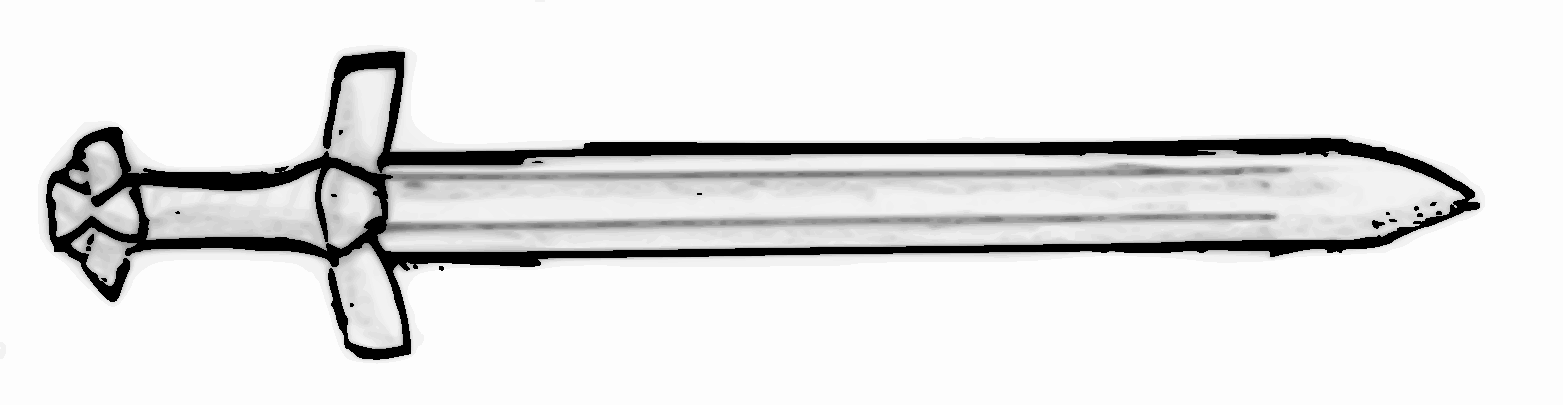
\includegraphics[width=\columnwidth]{vikingsword.pdf}\label{vikingsword}

\paragraph{Dedicated Power:} A dedicated power must be related to pursuit of its special purpose and activates upon a successful attack against an eligible creature.  The creature is allowed a saving throw vs. spell to avoid the effect.  The GM makes the determination of whether a creature is eligible.  An intelligent weapon can refuse to activate its dedicated power, even if its wielder is dominant.  A dedicated power acts as if cast by an 8th level spell caster.

\noindent \begin{minipage}{\columnwidth}

\captionof{table}{Dedicated Powers}\label{dedicatedpowers}
\noindent \begin{tabular}{|p{.15\columnwidth}|p{.5\columnwidth}|p{.2\columnwidth}|}
\hline
1d100	& Dedicated Power	& XP Bonus \\
\hline\hline
\rowcolor[gray]{0.9}01--10	& Blindness---2d6 rounds	& +100 \\
11--20	& Confusion---2d6 rounds	& +100 \\
\rowcolor[gray]{0.9}21--25	& Disintegrate	& +200 \\
26--55	& Fear---1d4 rounds	& +100 \\
\rowcolor[gray]{0.9}56--65	& Permanent insanity	& +200 \\
66--80	& Paralysis---1d4 rounds	& +150 \\
\rowcolor[gray]{0.9}81--00	& Simultaneous Chant and Prayer---2d4 rounds	& +100 \\
\hline
\end{tabular}

\end{minipage}

\paragraph{Weapon Ego:} After all other aspects of a weapon have been recorded, the GM calculates an intelligent weapon's total ego points.  

\noindent \begin{minipage}{\columnwidth}

\captionof{table}{Weapon Ego Points}\label{weaponego}
\noindent \begin{tabular}{|p{.65\columnwidth}|p{.25\columnwidth}|}
\hline
Weapon Attributes	& Ego Points \\
\hline\hline
\rowcolor[gray]{0.9}Enchantment bonus	& 1/bonus* \\
Each detection power	& 1** \\
\rowcolor[gray]{0.9}Each extraordinary power	& 2** \\
Special purpose	& 5 \\
\rowcolor[gray]{0.9}Each spoken language	& 1 \\
Telepathic 	& 2 \\
\rowcolor[gray]{0.9}Read spoken languages	& 1 \\
\textit{Read magic}	& 2 \\
\hline
\end{tabular}
\noindent\begin{tabular}{p{.95\columnwidth}}
*If the weapon has multiple enchantment bonuses, it gains 1 ego point for its lowest and highest enchantment bonuses.  For example, a \textit{+1 flame tongue} would gain 5 ego points.  Intelligent swords with special powers double enchantment bonus ego points. \\
**If a power is doubled or tripled, count ego points two or three times. \\
\end{tabular}\vspace{.5em}

\end{minipage}

Ego points combined with weapon's intelligence represent an intelligent weapon's force of personality.  A weapon with high ego points has a very dominant personality.  

\paragraph{Personality Conflicts:} An intelligent weapon will always act in perfect accordance with its stated alignment and towards the ends of its special purpose (if any).  If the wielder's actions disagree with the weapon's alignment or special purpose, a personality conflict will occur.  A weapon with 19 or more ego points will always feel superior to its wielder, and a personality conflict occurs anytime such a weapon and its wielder disagree for any reason.  Personality conflicts are also more common when the weapon's alignment has any component of neutral and the wielder's alignment is not an exact match.

To determine the force of the wielder's personality add together his intelligence, charisma and highest class level or HD.  The result is the wielder's personality score when he is at full strength.  If he is wounded, he suffers penalties to his personality score.  The wielder suffers a $-1$ penalty each time he loses a number of hit points equal to his total hit points divided by his highest class level or HD (rounded up).  

When a personality conflict occurs, the weapon's personality score is compared to the wielder's current personality score.  If the weapon has a higher score, it dominates the wielder and can force him to perform actions against his will.  These actions should always be well thought out and are often in accordance with the sword's alignment and/or special purpose.  Should an item gain dominance over its wielder, it resists his desires.  In addition, it can demand concessions such as any of the following:

\begin{itemize}
\item Removal of associates whose alignment or personality is distasteful to the weapon.

\item Disposal of all other magic items or items of a certain type.

\item Obedience from the wielder allowing the weapon to direct his movements.

\item Immediately seek out and attempt to slay the weapon's hated enemy.

\item Magical and mundane protections for when the weapon is not in use.

\item In the future, the wielder must carry the weapon at all times.

\item The wielder must relinquish the weapon to a more suitable wielder due to alignment differences or other disagreements.
\end{itemize}

In extreme cases of personality conflicts, the weapon can also force the character to perform the following actions: 

\begin{itemize}
\item Enter into combat.

\item Stop attacking his opponents.

\item Attack himself or his associates.

\item Surrender to an opponent.

\item Drop the weapon.
\end{itemize}

Naturally, such actions are unlikely when harmony reigns between the wielder and his weapon or when their purposes and alignments are well matched.  Even so, a weapon may seek out a more powerful wielder with a lower personality score in order to easily establish and maintain dominance over him and better accomplish its special purpose.   

All intelligent magical weapons desire to play an important role in whatever activity is under way, particularly combat.  Such weapons are often rivals of each other, or friendly rivals if they are of the same alignment.  No intelligent weapon wants to share its wielder with any other.  An intelligent weapon is aware of the presence of any other of its kind within 60 feet, and most intelligent weapons attempt to mislead or distract their wielder so that he ignores or destroys the rival weapon.  

Intelligent weapons are never totally controlled or silenced by their wielders.  Even though the weapon may never successfully control its wielder, it remains undaunted and continues to express its wishes and demands. 

These guidelines only cover intelligent magical weapons, however, the GM may create intelligent magical items of a non-weapon nature.  The GM must determine their powers and special purposes on a case-by-case basis. 
 
\section{ARTIFACTS \& RELICS}

\index{Artifacts \& Relics}These objects are extremely rare items of ancient power and majesty.  They are incredibly more powerful than even the greatest of the known magical items.  Artifacts are the mightiest magical items, crafted in the mists of time by the most renowned wizards in history, while relics are awesome items of great power associated with, or formerly a part of, a highly venerated (or most reviled) priest from days of old.  

These are legendary items and the epitome of magical power in the game, so their use must be strictly controlled.  They must be few in number across a campaign world, and gaining possession of one should require an epic monumental adventure suitable only for the most powerful characters.  It is suggested that single classed human characters within an adventuring group have an average character level of at least 15 before an artifact or relic is introduced into play.  It is advised that if a player character gains possession of one, it should be for the purpose of completing a major quest or campaign goal, and the GM should not allow him to keep it for very long.  Artifacts and relics are intelligent, and known to mysteriously disappear when they are no longer needed.

\paragraph{General Characteristics:} Each artifact or relic is a unique item.  A GM must specifically place an artifact or relic in their individual campaigns.  They will not be found on random treasure tables.  They cannot be transferred between campaign worlds, except in highly unusual circumstances that the GM must approve.

The GM designs artifacts and relics to fit his world, and he alone knows the extent of the powers that they possess, as well as the command words and gestures needed to activate them.  The GM has free reign to give the artifacts and relics any power he desires, even if the power would normally be considered god-like.  In addition to having powers of lesser and greater effect, artifacts and relics are cursed.  Just activating an artifact or relic can result in a dangerous or even deadly side effect being triggered, and simply possessing an artifact or relic is to risk insanity or worse.  Their effects are permanent, and subject only to divine intervention from the most powerful deities.

These items are nearly indestructible, and very few effects have even a slight chance to affect them.  Unique and elaborate means are required to destroy one.

\paragraph{Physical Description:} The first thing to do when creating an artifact or relic is to decide its form.  This can be anything chosen from the standard magical item tables or equipment tables, such as a book, jewelry, clockwork toy, cloak or robe, boots or shoes, weapon, armor, masks, lenses, mummified body parts, magical shelters, statues, vehicles or anything else the GM can imagine.  Regardless of its physical form, an artifact or relic never expends charges; its powers are permanent.

\paragraph{Origins and History:} The next step when creating an artifact or relic is to determine its history.  The GM must first decide who created the item and for what purpose.  The item is assumed to have been crafted in ancient times and will have a history in which fact becomes impossible to separate from myth and legend.  This item was once possessed by a deity or his most powerful mortal follower, and was often crafted for an express purpose, such as for use by a particular hero or to fight a particular foe.  

This purpose may have been fulfilled a long time in the past, or it maybe a never-ending or self-renewing purpose.  The item is so closely associated with its purpose that its powers might only be fully activated by creatures who meet certain class and/or racial criteria, or it may reveal its full powers only when dealing with a specific threat.

Next, the GM must roughly determine what has happened to the item over the centuries.  He should note when and where it has appeared and what events occurred after its appearance.  Finally, the GM fills in details in the item's history with clues to its powers and any legends (both true and false) that have come to surround the item.  

\paragraph{Alignment:} Artifacts and relics always radiate a strong alignment aura when \textit{detect evil/good}, \textit{know alignment} or similar is cast.  The GM selects the most appropriate alignment for the artifact.

\paragraph{Lesser Powers:} Using the item's history as a guide, the GM begins to assign powers to the artifact or relic, starting with the least of them.  

\paragraph{ Greater Powers:} After selecting the lesser powers, the GM then selects the item's greater powers.  Artifacts and relics will have no more than two greater powers.  Often, greater powers can only be activated when doing so is directly related to the item's purpose, and these can often be revealed in the item's history.  Though the exact means of activating the greater powers and the item's purpose may be ambiguous.  

\paragraph{Dangerous Side Effects:} After providing the artifact or relic with its lesser and greater powers, the GM must determine the dangers inherent in its use.  Activating any of the powers of an artifact or relic carries grave risks.  Creatures possessing great will and incredible power originally crafted and used the item, and even they placed themselves in danger to activate the item's powers.  Naturally, these dangerous side effects will be at best only hinted at in the item's history.  

\paragraph{Curse of Insanity:} Ultimately, every artifact and relic brings insanity to its possessor.  Even if the item is never used, its possessor becomes paranoid and jealously possessive of the item.  Soon, the possessor becomes delusional and begins to see threats where none exist.  Eventually, the insanity causes the possessor of the item to attempt to destroy their allies and associates (either openly or covertly), believing them to be enemies out to kill him and/or steal the artifact.

\paragraph{How to Destroy it:} Lastly, the GM must determine a means to destroy the artifact or relic.  Since an artifact or relic is nearly indestructible, destroying one is next to impossible.  It is impervious to all mundane and most magical attacks.  It cannot be crushed, dissolved in acid, melted or broken.  Even in the rare event that a magical attack succeeds or some way is found to destroy the item's physical form, the item is only disrupted for a (relatively) short time, but within a century, the item reforms in another location with all of its powers and dangerous side effects restored.  To truly destroy the item, a creature must complete a very specific and demanding set of conditions that are as unique as the artifact itself.

\end{multicols}



